 \documentclass[ %
    11pt, %
    a4paper, %
    BCOR=12mm, %
    DIV=12, %
    headsepline=true, %
    parskip=half, %
    %draft=true, %
]{article}
\let\chapter\section 
\let\section\subsection 
\let\subsection\subsubsection 
\let\subsubsection\paragraph 
\let\paragraph\subparagraph 

\usepackage{amssymb,amsmath}
\usepackage{engrec}
\usepackage[british,UKenglish,USenglish,english,american]{babel}
\usepackage[latin1]{inputenc}
\usepackage{enumerate}
\usepackage{empheq}
\usepackage{picins}
\usepackage{floatflt}
\usepackage{graphicx}
\graphicspath{{images/}}%% Allgemeine Bilder
\usepackage{color}
\usepackage{natbib}
\usepackage{pdfpages}
\usepackage{hyperref}


\begin{document}


\begin{titlepage}

\begin{center}




\includegraphics[width=0.3\textwidth]{Bilder/logo}\\[1.2cm]    

\textsc{\LARGE Albert-Ludwigs-Universit\"at Freiburg}\\[1.75cm]

\textsc{\Large Physikalisches Fortgeschrittenen-Praktikum I}\\[0.75cm]



\newcommand{\HRule}{\rule{\linewidth}{0.5mm}}
\HRule \\[0.5cm]
{ \huge \bfseries Szintillationszähler}\\[0.5cm]

\HRule \\[1.75cm]


\begin{minipage}{0.4\textwidth}
\begin{flushleft} \large
\emph{Studenten:}\\
Daniel \textsc{Uhl}\\ \setlength{\parindent}{1.25cm} \& 
\setlength{\parindent}{0cm} \\ Jan P\'eter \textsc{Szabados} 
\end{flushleft}
\end{minipage}
\hfill
\begin{minipage}{0.4\textwidth}
\begin{flushright} \large
\emph{Tutor:} \\
Matthias \textsc{Gorzellik}\\
\end{flushright}
\end{minipage}

\vfill


{\large \today}

\end{center}

\end{titlepage}

\tableofcontents
\chapter{TASK}
\section{Measuring the bandgap of Si and Ge} 
1. Optimizing the beam path. \\
2. Measuring the absorption and transmission spectrum of silicon and germanium respectively. \\
3. Underground measurement with covered sample. \\
4. Measuring spectra of the lamp used with both lattices. \\
5. Determining the bandgap energy of Si and Ge using their absorption and transmission spectra. \\
\section{Haynes-Shockley-experiment} 
1. Observation and measurement of a cloud of charged carriers'(created in p-type Ge using a laser pulse) development in time and space. \\
2. Determining the mean lifetime of the free electrons using the time development of the signal amplitude. \\
3. Determining the mobility of the free electrons using the time development of the center of the signal. \\
4. Determining the diffusion constant using the time development of the signal's shape.\\
\section{Semiconductor detectors} 
1. Measuring the spectra of Co-57 and Am-241 with a CdTe- and a Si-detector respectively. \\
2. Underground measurement of both the CdTe- and the Si-detector. \\
3. Determining the relation of absorption probabilities of the two detectors using the relation of their peak heights (at the same energy). \\
4. Determining the relative energy resolution using position and width of the peaks.
\chapter{THEORETICAL BACKGROUND}
\section{Interaction of photons or $\gamma$-quanta with matter}
\subsection*{Photoelectric effect}
The \textit{photoelectric effect} describes the effect of a $\gamma$-quantum interacting with matter. If the energy of the photon $\mathit{E_{\gamma}=h\nu}$ is higher than the electron binding energy (the work function) of the material, the electron is ejected. If the energy is too low the electron is not able to escape. In case of the ejection the electron has the energy $\mathit{E_{e^{-}}=h\nu-E_{D}}$ and leaves a free place in the electron shell. Because of the lower energy an electron of a higher shell falls down in that free spot by emitting a photon or an Auger-electron. The cross-section of the \textit{photoelectric effect} is defined as $\mathit{\rho_{photo}\propto Z^{5}/E^{\frac{7}{2}}}$.

\subsection*{Compton scattering}
If a $\gamma$-quantum hits an outer or a free electron and they perform an inelastic scattering so that the $\gamma$-quantum gives a part of its energy to the electron, it is called \textit{Compton Scattering}. The deflection angle $\theta$ depends on the energy of the $\gamma$-quantum. The probability of this effect taking place increases with the atomic number $\mathit{Z}$ of the absorbing material as well as at an energy of 200 keV to 5 MeV.

\subsection*{Pair production}
At an energy of 1.022 MeV and above there is another effect, the \textit{Pair production}. At that point the energy of the $\gamma$-quantum is as high as the energy of a positron-electron-pair at zero velocity. So a pair of these could be excited in the field of an electron or an nucleus. The free positron annihilates when reaching the surrounding matter by sending out two $\gamma$-quanta with energy of 0.511 MeV per quantum.

\section{Interference of photons}
As is known there could be interference effects with photons for example when photons pass through a grid. That effect could also be  appearing with single photons, as is known from quantum physics.

\section{Semiconductor and single-element semiconductor}
\textit{Semiconductor} are materials whose conductivity or rather electrical resistance is related to a parameter which depends on the temperature. \textit{single-element semiconductor} are \textit{semiconductor} out of one single material; for example germanium or silicon.

\section{Band structure}
The \textit{Band structure} is a model of quantum physics and helps to distinguish between conductor, semiconductor and insulator. In that model we use an energy level called valence band where the electrons normally are and a higher energy level called the conduction band. The energy difference between these two bands is the bandgap. In a conductor the energy level of valence and conduction band crosses partly or completely so there is no band gap. In a semiconductor the electron can cross the band gap by getting energy and in an insulator the bandgap is normally too big for an electron to cross it.\\
\begin{figure}[h]
\begin{center}
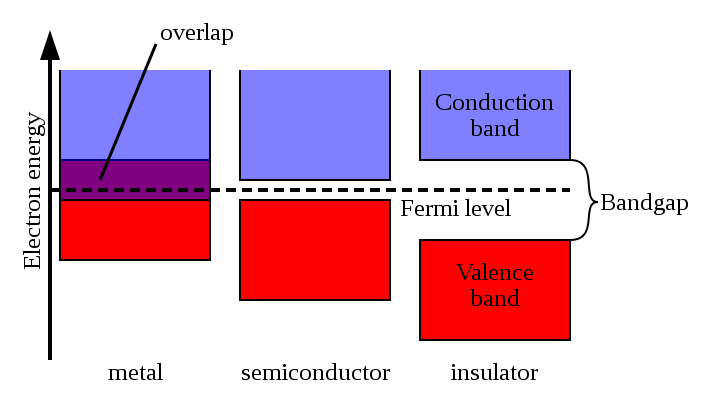
\includegraphics[scale=0.3]{bilder/isolator-metal}
\caption{ Band structure of a conductor, semiconductor and insulator. Source:[sclo] }
\label{fig:band}
\end{center}
\end{figure}
\\
A semi-classical way to describe the model: You can observe two atoms which are placed far away from each other. Their electrons have discrete levels of energy. If you decrease the distance between these electrons that leads to an interaction and the wave-functions of those electrons overlap. The Pauli exclusion principle gives us now a separation in two
\begin{figure}[h]
\begin{center}
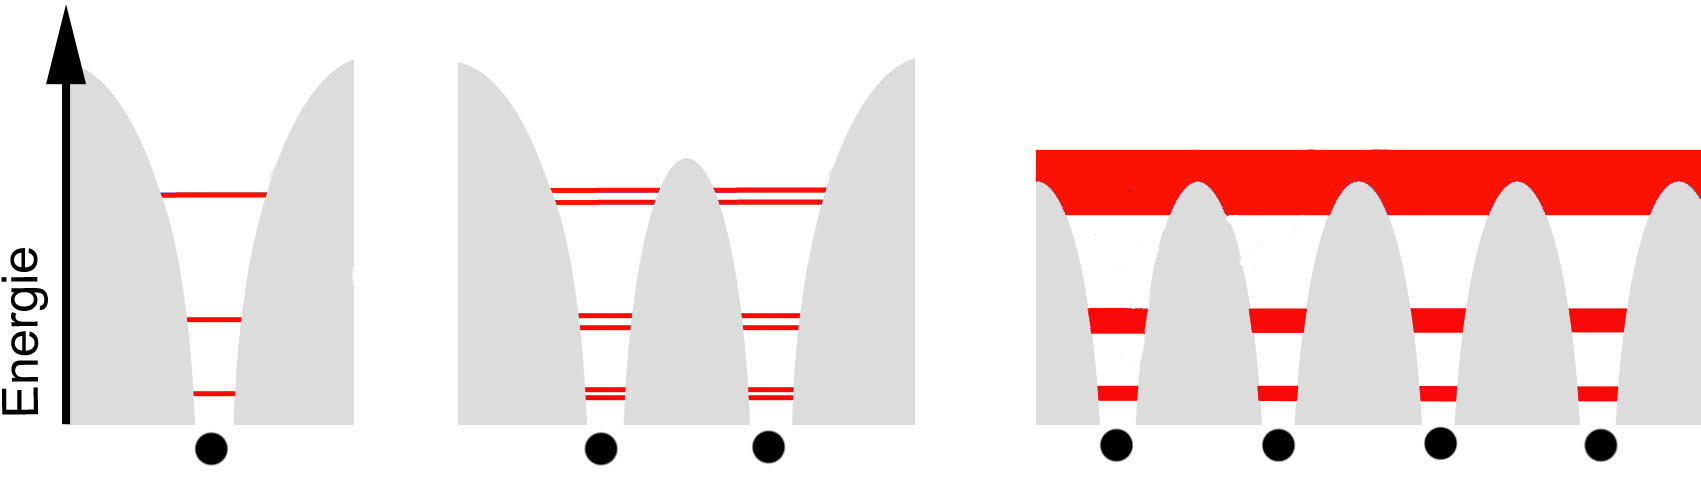
\includegraphics[scale=0.2]{bilder/energieniveaus-pauli}
\caption{Energy levels of: 1.single atom, 2.two atoms, 3.solid state body. Source:[Amr] }
\label{fig:pauli}
\end{center}
\end{figure}
\\
slightly separated energy levels, what leads, because of the high count of electrons, to continuous energy bands.
\section{Charge carrier in semiconductor}
If an electron moves to the conduction band it leaves a free spot in the valence band. That spot can be seen as an positive charge carrier. So there are negative electron and positive charge carriers in a semiconductor. If an external voltage is applied, the electrons move in the direction of the positive pole and the free spots in the direction of the negative pole.
\begin{figure}[h]
\begin{center}
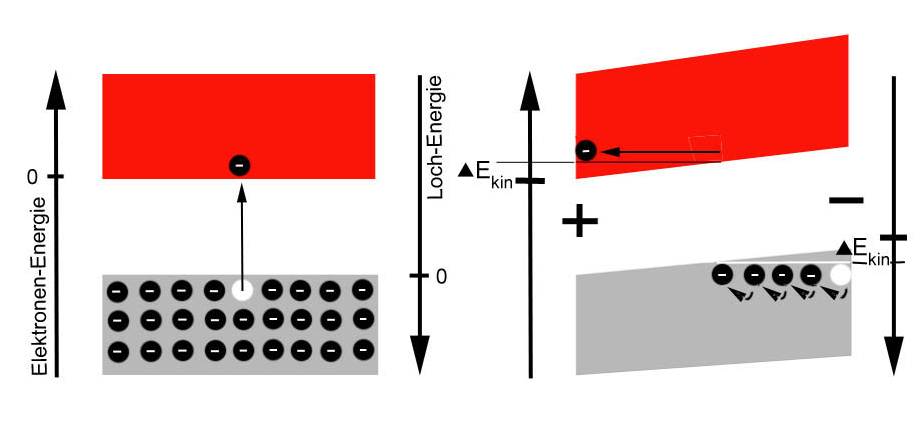
\includegraphics[scale=0.3]{bilder/ladungstraeger}
\caption{Band crossing (left) and external voltage (right). Source:[Amr] }
\label{fig:ladungs}
\end{center}
\end{figure}
\\
\section{Exponential decay and mean lifetime}
The time between the appearance of an electron-spot-pair and its recombination is called mean lifetime. If you now look at a lot of these events, you can describe the count of the not yet recombined pairs $\mathit{N(t)}$ after a time interval $\mathit{t}$ as an exponential decay:
\begin{center}
$\mathit{N(t)=N_{0}\cdot e^{-t/\tau}}$
\end{center}
Where $mathit{N_{0}}$ is the count of pairs at $mathit{t=0}$ and $mathi{\tau}$ is the average lifetime. If there is an external voltage, the average lifetime is now important to calculate the average velocity of the charge carrier:
\begin{center}
$\mathit{\vec{v}_{p/n}=\pm\frac{e\tau}{m_{p/n}}\vec{E}=\pm\mu_{p/n}\vec{E}}$
\end{center}
$\mathit{p/n}$ is the type of the charge, $\mathit{m}$ is the mass of the charge carrier an $\mathit{\mu}$ the mobility of the carrier.
\section{Direct and indirect semiconductor}
In the wavenumber space we can observe the energy in relation to its wavenumber. The upper line of the valence band and the bottom line of the conduction band are now no longer parallel. You can now differentiate between the direct semiconductor where the maximum of the valence band lies directly under the minimum of the conduction band and the indirect semiconductor where that extrema are shifted by  $\mathit{\delta\vec{p}}$.
\begin{figure}[h]
\begin{center}
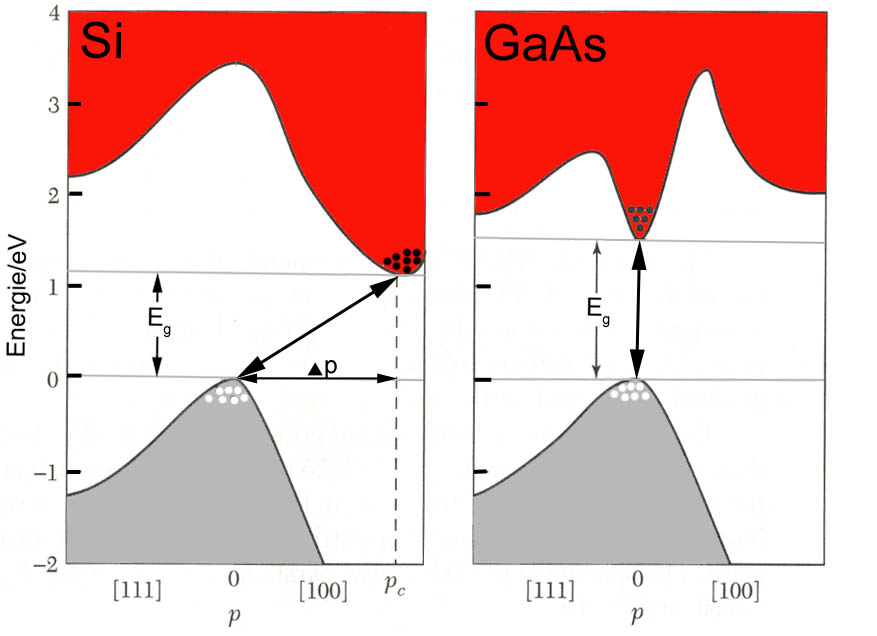
\includegraphics[scale=0.3]{bilder/impulsraum}
\caption{indirect semiconductor (left) and direct semiconductor (right). Source:[Amr] }
\label{fig:impuls}
\end{center}
\end{figure}
\\
\section{Intrinsic and extrinsic semiconductor, Doping}
\textit{Intrinsic semiconductor} are semiconductors with a perfect crystal structure without any errors or contamination. It is not possible to create crystals like these. Real semiconductors have contaminations and defects in the structure. At the structure of the crystal there could be parts of the structure defect or displaced. Because of that, there could be new band levels and the band gap could be distorted. Foreign atoms could also cause errors.
\subsection*{Doping}
Volitional contamination with atoms with more or less valence electrons as the atoms of the crystal is called \textit{doping}. A foreign atom with an electron more is called a \textit{donor} and one with an electron less is called \textit{acceptor}. Additional electrons are not implemented in the crystal structure and can be seen as free electrons for the conduction band. Missing electrons are free spots and can be seen as free positive charge carriers.\\
The contamination with donors is a p-doping and with acceptors is a n-doping. The specific conductivity could grow by doping a semiconductor.
\section{p-n-Diode, Use as semiconductor detector}
If you put a p-doped and an n-doped together (in contact) free electrons diffuse from the n-layer in the free spots in the p-layer at the contact area. Because of that, the free charges get balanced out in that area. The kernel can't get out of the crystal structure, so after that balancing there are positive kernels left in the n-doped layer and negative kernels left in the p-doped layer, whereby an electric field develop in that area. This is called contact electrification with the voltage $\mathit{U_{bi}}$.\\
Is a charge generated by an outer stimulation, generated charges will be accelerated and leave the depletion layer. For the usage as a semiconductor detector you can use such a diode. If a photon passes the depletion layer, an electric current will be generated because of the photo- or Compton-effect.
\begin{figure}[h]
\begin{center}
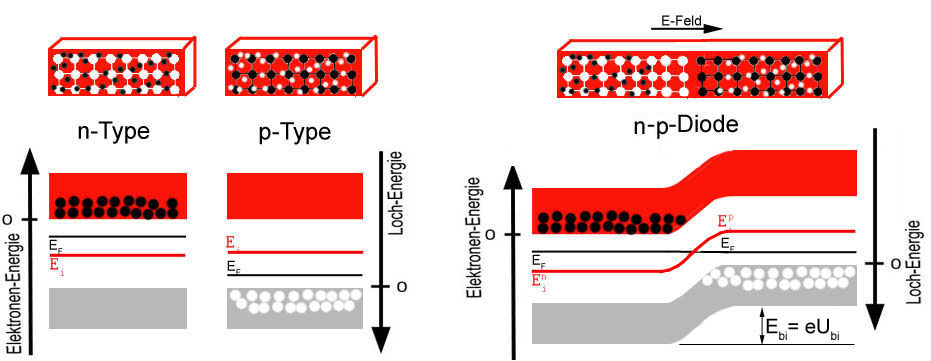
\includegraphics[scale=0.5]{bilder/diode}
\caption{Semiconductor layer (left), diode (right). Source:[Amr] }
\label{fig:diode}
\end{center}
\end{figure}
\section{Electronics}
\subsection*{Preamplifier}
Preamplifiers cause a linear amplification of electric signals in detectors and other, similar electronic devices. Often these amplifiers are built-in.\\
\subsection*{Shaping Amplifier}
A shaping amplifier is an electronic amplifier which can shape the incoming signal. In this experiment, a $(CR)-(RC)^2$-SA is used. 
\subsection*{Multi Channel Analyzer}
An MCA is applied to record electronic signals of different voltage. It consists of many channels, which are connected to voltages linearly. This way incoming signals are matched with the appropriate channel.
\subsection*{Lock-In Amplifier}
The lock-in method is used to visualize weak signals in heavy noise. The incoming and a reference signal are applied to a synchron detector. The signals are multiplied, integrated with the help of a low-pass and eventually amplified. This way only the part of the incoming signal which has the same frequency and phase as the reference signal is let through.

\chapter{Experiment No.1: Measuring the bandgap}
\section{Description}
\textbf{Experimental Setup} \\
In this experiment we ought to determine the bandgap of the semiconductors germanium (Ge) and silicon (Si). To reach this goal, we put the semiconductors one after the other in a spectrometer, where the light of a lamp is split up (depending on the wavelengths of the photons making it up) with the help of a lattice. After crossing an aperture slot and a filter, which filters out IR and UV photons, the photons - when reaching the sample - get either absorbed or transmitted, depending on their energy. By measuring the transmission and absorption spectra we can determine the band gap of the sample. \\
\begin{figure}[h]
\begin{center}
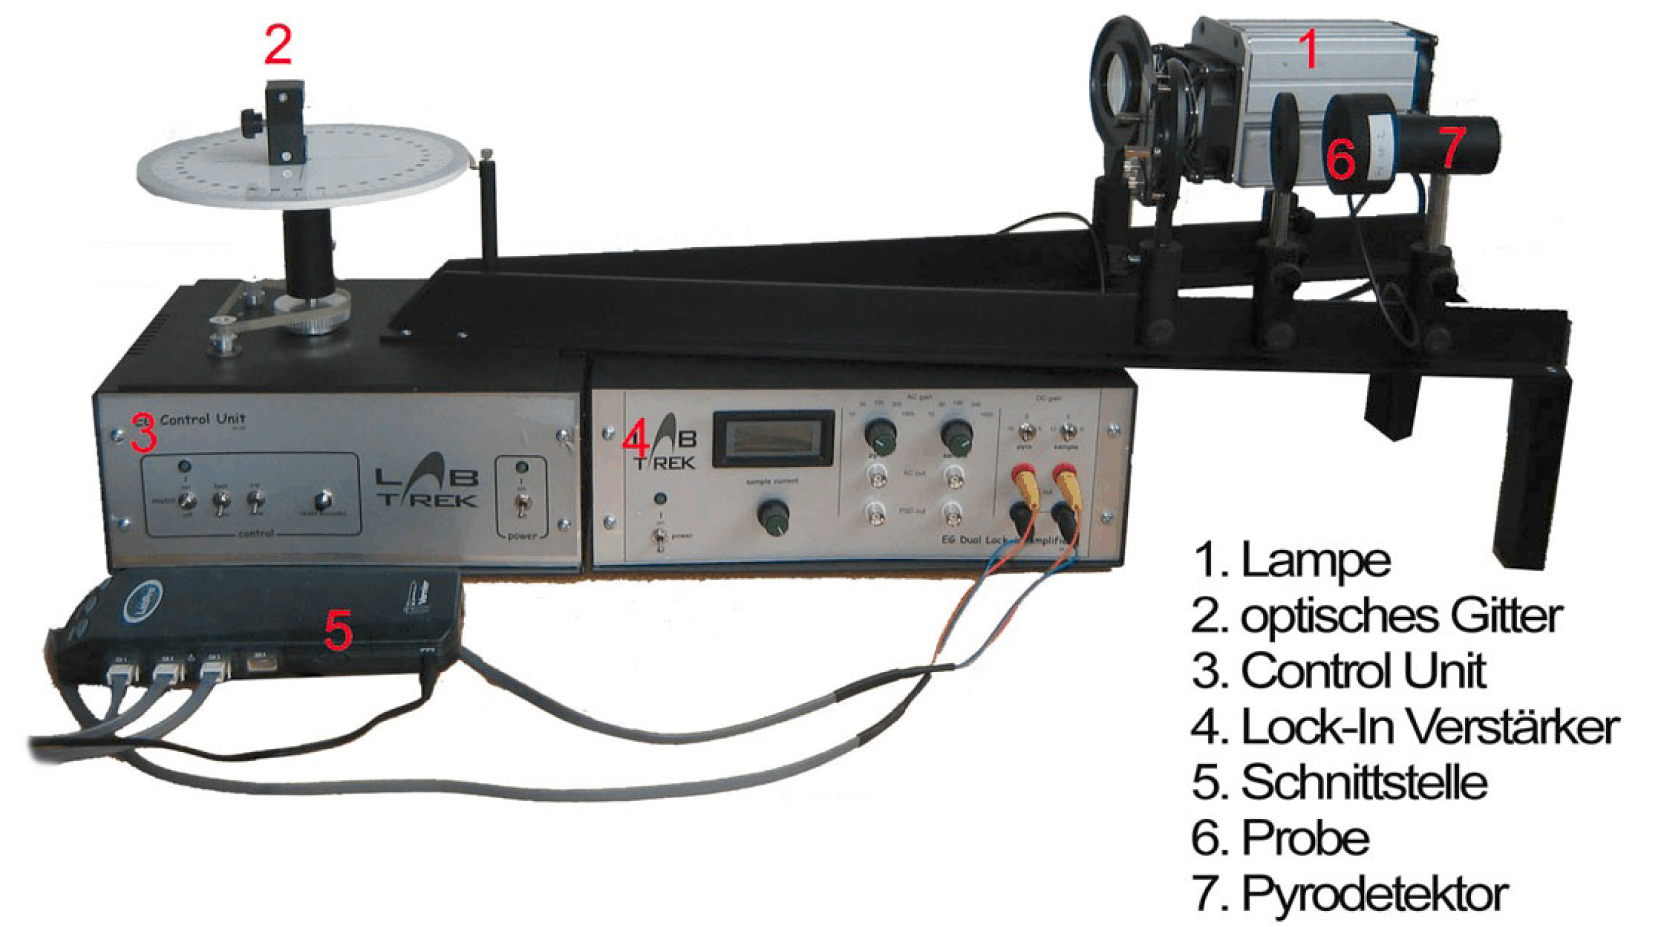
\includegraphics[scale=0.3]{Bilder/Spektrometer.png}\caption{Experimental setup. Source: [Ver]}
\label{spektrometer}
\end{center}
\end{figure}\\
The spectrometer can be seen in the picture above (\ref{spektrometer}). It consists of a lattice (2), which is exposed to light coming from a source (1). There's a chopper right in front of the source, so that the light emitted has a frequency of 70 Hz: that's how the computer can distinguish the source's signals from the signals created by the surrounding light. The 1st order diffraction maximum expands the spectrum: thanks to this, only photons of a specific wavelength (depending on the angle) cross the aperture slit. A small engine helps us measuring the spectra by providing a constant velocity. The absorption in the sample (6) can be measured with the help of the electric current. The transmission spectrum is measured using a pyrodetector (7) connected to a lock-in-amplifier (4), which has the frequency of the chopper as reference signal. \\
Both spectra and the angle (which is measured by the Control Unit(3)) get to the computer via the interface (5).\\
\textbf{Absorption spectrum}\\
Photons with a higher energy than the bandgap energy can excite electrons, so that they move from the valence to the conduction band. Of course this leads to a significant increase in the sample current. If a voltage is applied to the sample, the absorption can be measured with the help of its electric resistance.\\
\\
\textbf{Transmission spectrum}\\
The transmitted photons can be measured with the pyro detector, which detects only changes in the incoming signal. That's why a chopper is applied.\\
\\
\section{Analysis}
To get a transmission and an absorption coefficient, the background has to be substracted from the measured values. The result needs to be divided by the measured value of the source without sample, i.e. the value the pyro detector measures. The formulas for the spectra are the following:\\
\\
$Trans_{real}=\frac{Trans_{measured}-Background}{Lightsource}$\\  
\\                         $Absorp_{real}=\frac{Absorp_{measured}-Background}{Lightsource}$\\
\\
To determine the bandgap energy, we plotted the transmission and absorption spectra over the energy and did linear fits at the flanks of the curves. The intersection point of these linear fits with the horizontal lines through the maximum of the transmission spectrum (for the transmission) and the minimum of the absorption spectrum (for the absorption) provide us with a maximum and a minimum value of the bandgap energy. As we calculated the intersection points for both "negative" (because in the formula for the energy we have $E\propto\frac{1}{sin\theta}$) and positive energies, we get four values for each sample.\\
The energy and its error were calculated as follows:\\
$m*E+c=d$\\
$\Leftrightarrow E=\frac{d-c}{m}$\\
$\Rightarrow s_{E}=\sqrt{(\frac{\partial{E}}{\partial{d}})^2*s_{d}^2+(\frac{\partial{E}}{\partial{c}})^2*s_{c}^2+(\frac{\partial{E}}{\partial{m}})^2*s_{m}^2}=\sqrt{\frac{s_{d}^2}{m^2}+\frac{s_{c}^2}{m^2}+\frac{(d-c)^2}{m^4}*s_{m}^2}$\\
\\
The results are the following:\\
\begin{table}[htbp]
  \centering
  \caption{Results}
    \begin{tabular}{rrrrr}
    $Sample$ & $E_{trans}$  & $s_{E_{trans}}$ & $E_{absorp}$ & $s_{E_{absorp}}$ \\
    Si    & -1,10  & 0,08  & -1,08 & 0,03 \\
    Si    & 1,11  & 0,04  & 1,04  & 0,03 \\
    Ge    & -0,64 & 0,06  & -0,65 & 0,08 \\
    Ge    & 0,63  & 0,05  & 0,63  & 0,04 \\
    \end{tabular}%
  \label{tab:addlabelx}%
\end{table}%
\\
All results are in eV. The plots are in the appendix. \\
Using these results, the weighted mean was calculated as follows (with the "negative" energies being positive in this calculation):\\
$\overline{E_{Si}}=\sum_{i=1}^{4}\frac{\frac{E_{i}}{s_{i}^2}}{\frac{1}{s_{i}^2}}}=1,087 eV$\\
$s_{\overline{E_{Si}}}=\sqrt{\frac{1}{\sum_{i=1}^{4}s_{i}^2}}=0,018 eV$\\
\\
The same equations hold for Ge too.\\
$\Rightarrow \overline{E_{Ge}}=(0,64\pm0,03) eV$\\
\\
The literature values given in [Ver] were $E_{Si}=1,12 eV$ and $E_{Ge}=0,66 eV$.\\
Our results are two(for Si) and one (for Ge) root-mean-square errors from the respective literature values. This is a good result, especially regarding the fact, that the calculations for the absorption and transmission coefficients had to be made without having measured values for both sample and source at the same angle. Of course the difference of the angles is really small, still, it's not necessarily 0: for that reason we have a systematic error in this part of the experiment. Also, we didn't have any errors given on parts of our spectrometer such as the interface, the cables, the pyrodetector, the lock-in-amplifier or the Control Unit. Another errors might have resulted from not taking into account the width of the aperture slit and the effect of the clearly visible fingerprint on the lattice in the Si-experiment.\\
\\
We can state that the error is too low on our results. Still, they are very close to their respective literature values, making the negligence of the errors listed above seem reasonable.



\chapter{Experiment No.2: The Haynes and Shockley-Experiment}
\section{Description}
\subsection*{Experimental Setup}
In this experiment we should determine the behavior of charge carriers in materials. Our material was Germanium. First we need free charge carrier to observe. To get them we use a laser to geht electron (our charge carrier) from the valence band to the conduction band. The laser is activated in short periodic impulses so we get little cluster of electrons. A voltage applied on the Ge accelerate our electron clusters in its electric field. To detect the cluster we using a detector so we could visualize the signal on an oscilloscope. Impuls and measuring happens 30 times per second (30Hz).
\begin{figure}[h]
\begin{center}
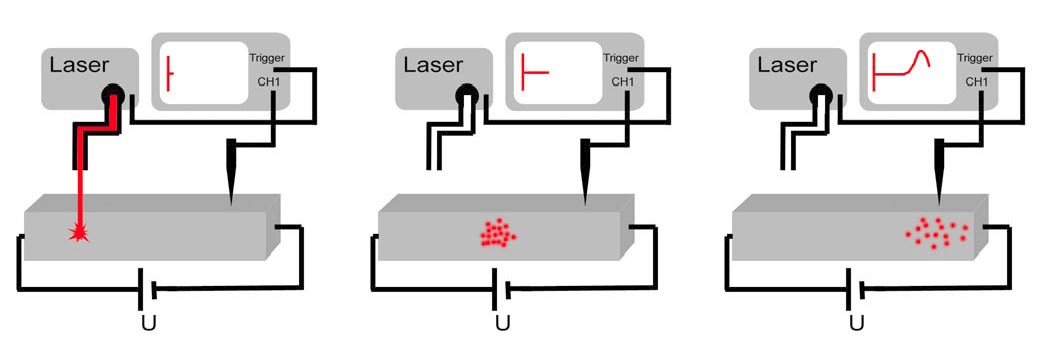
\includegraphics[scale=0.5]{Bilder/aufbau_teil2}
\caption{Experimental setup. Source:[Ver] }
\label{fig:aufbau2}
\end{center}
\end{figure}
\section{Analysis}
To get the mean time $\mathit{\tau}$, the mean free path and the mass diffusivity $\mathit{D_{e}}$ of the electrons in our p-Ge, we fitted normal distribution on the measured electron clusters of the oscilloscope. The normal distribution is given as:\\
\begin{center}
$\mathit{c(x)=A\frac{1}{\sqrt{2\pi \sigma^2}}}\exp\left(-\dfrac{(x-x_{c})^2}{2\sigma^2}\right)$
\end{center}
$\mathit{A}$,$\mathit{x_{c}}$ and $\mathit{\rho}$ are the known parameter of a normal distribution.\\
\\
The differential equation of an electron in a p-doped semiconductor is given as followed:\\
\begin{center}
$\mathit{c(t,x)=C\exp(-t/\tau_{n})\frac{1}{\sqrt{4\pi D_{e}t}} \exp\left(-\dfrac{(x-\mu_{n}Et)^2}{4D_{e}t}\right)}$
\end{center}
$\mathit{C}$ : Constant\\
$\mathit{\tau_{n}}$ : Mean time\\
$\mathit{D_{n}}$: Mass diffusivity\\
$\mathit{\mu_{n}}$ : Mobility of the free electrons\\
$\mathit{E}$ : Electrical field strength\\

Compare now the parameter of these two functions, it's easy to find the followed relationships:
\begin{tabbing}
$\mathit{x_{c}(t)=\mu_{n}Et}$,\\
$\mathit{A(t)=C \exp(-t/\tau_{n})}$,\\
$\mathit{\sigma(t)=\sqrt{2D_{n}t}}$,\\
\end{tabbing}
To get $\mathit{\mu_{n}}$, $\mathit{\tau_{n}}$ and $\mathit{D_{n}}$ we can fit these relations and get them from the parameter of the fits.
This approach works for the first series of measurements as well as for the second. 
\newpage
\subsection*{1. Measurements}
We put the normal distribution in the appendix, because of the big number of fits. Out of that fit we got our parameter for the following fits.
To get the mobility $\mathit{\mu_{n}}$ we can use the linear relation with the distance between laser and detector on the Ge.
\begin{figure}[h]
\begin{center}
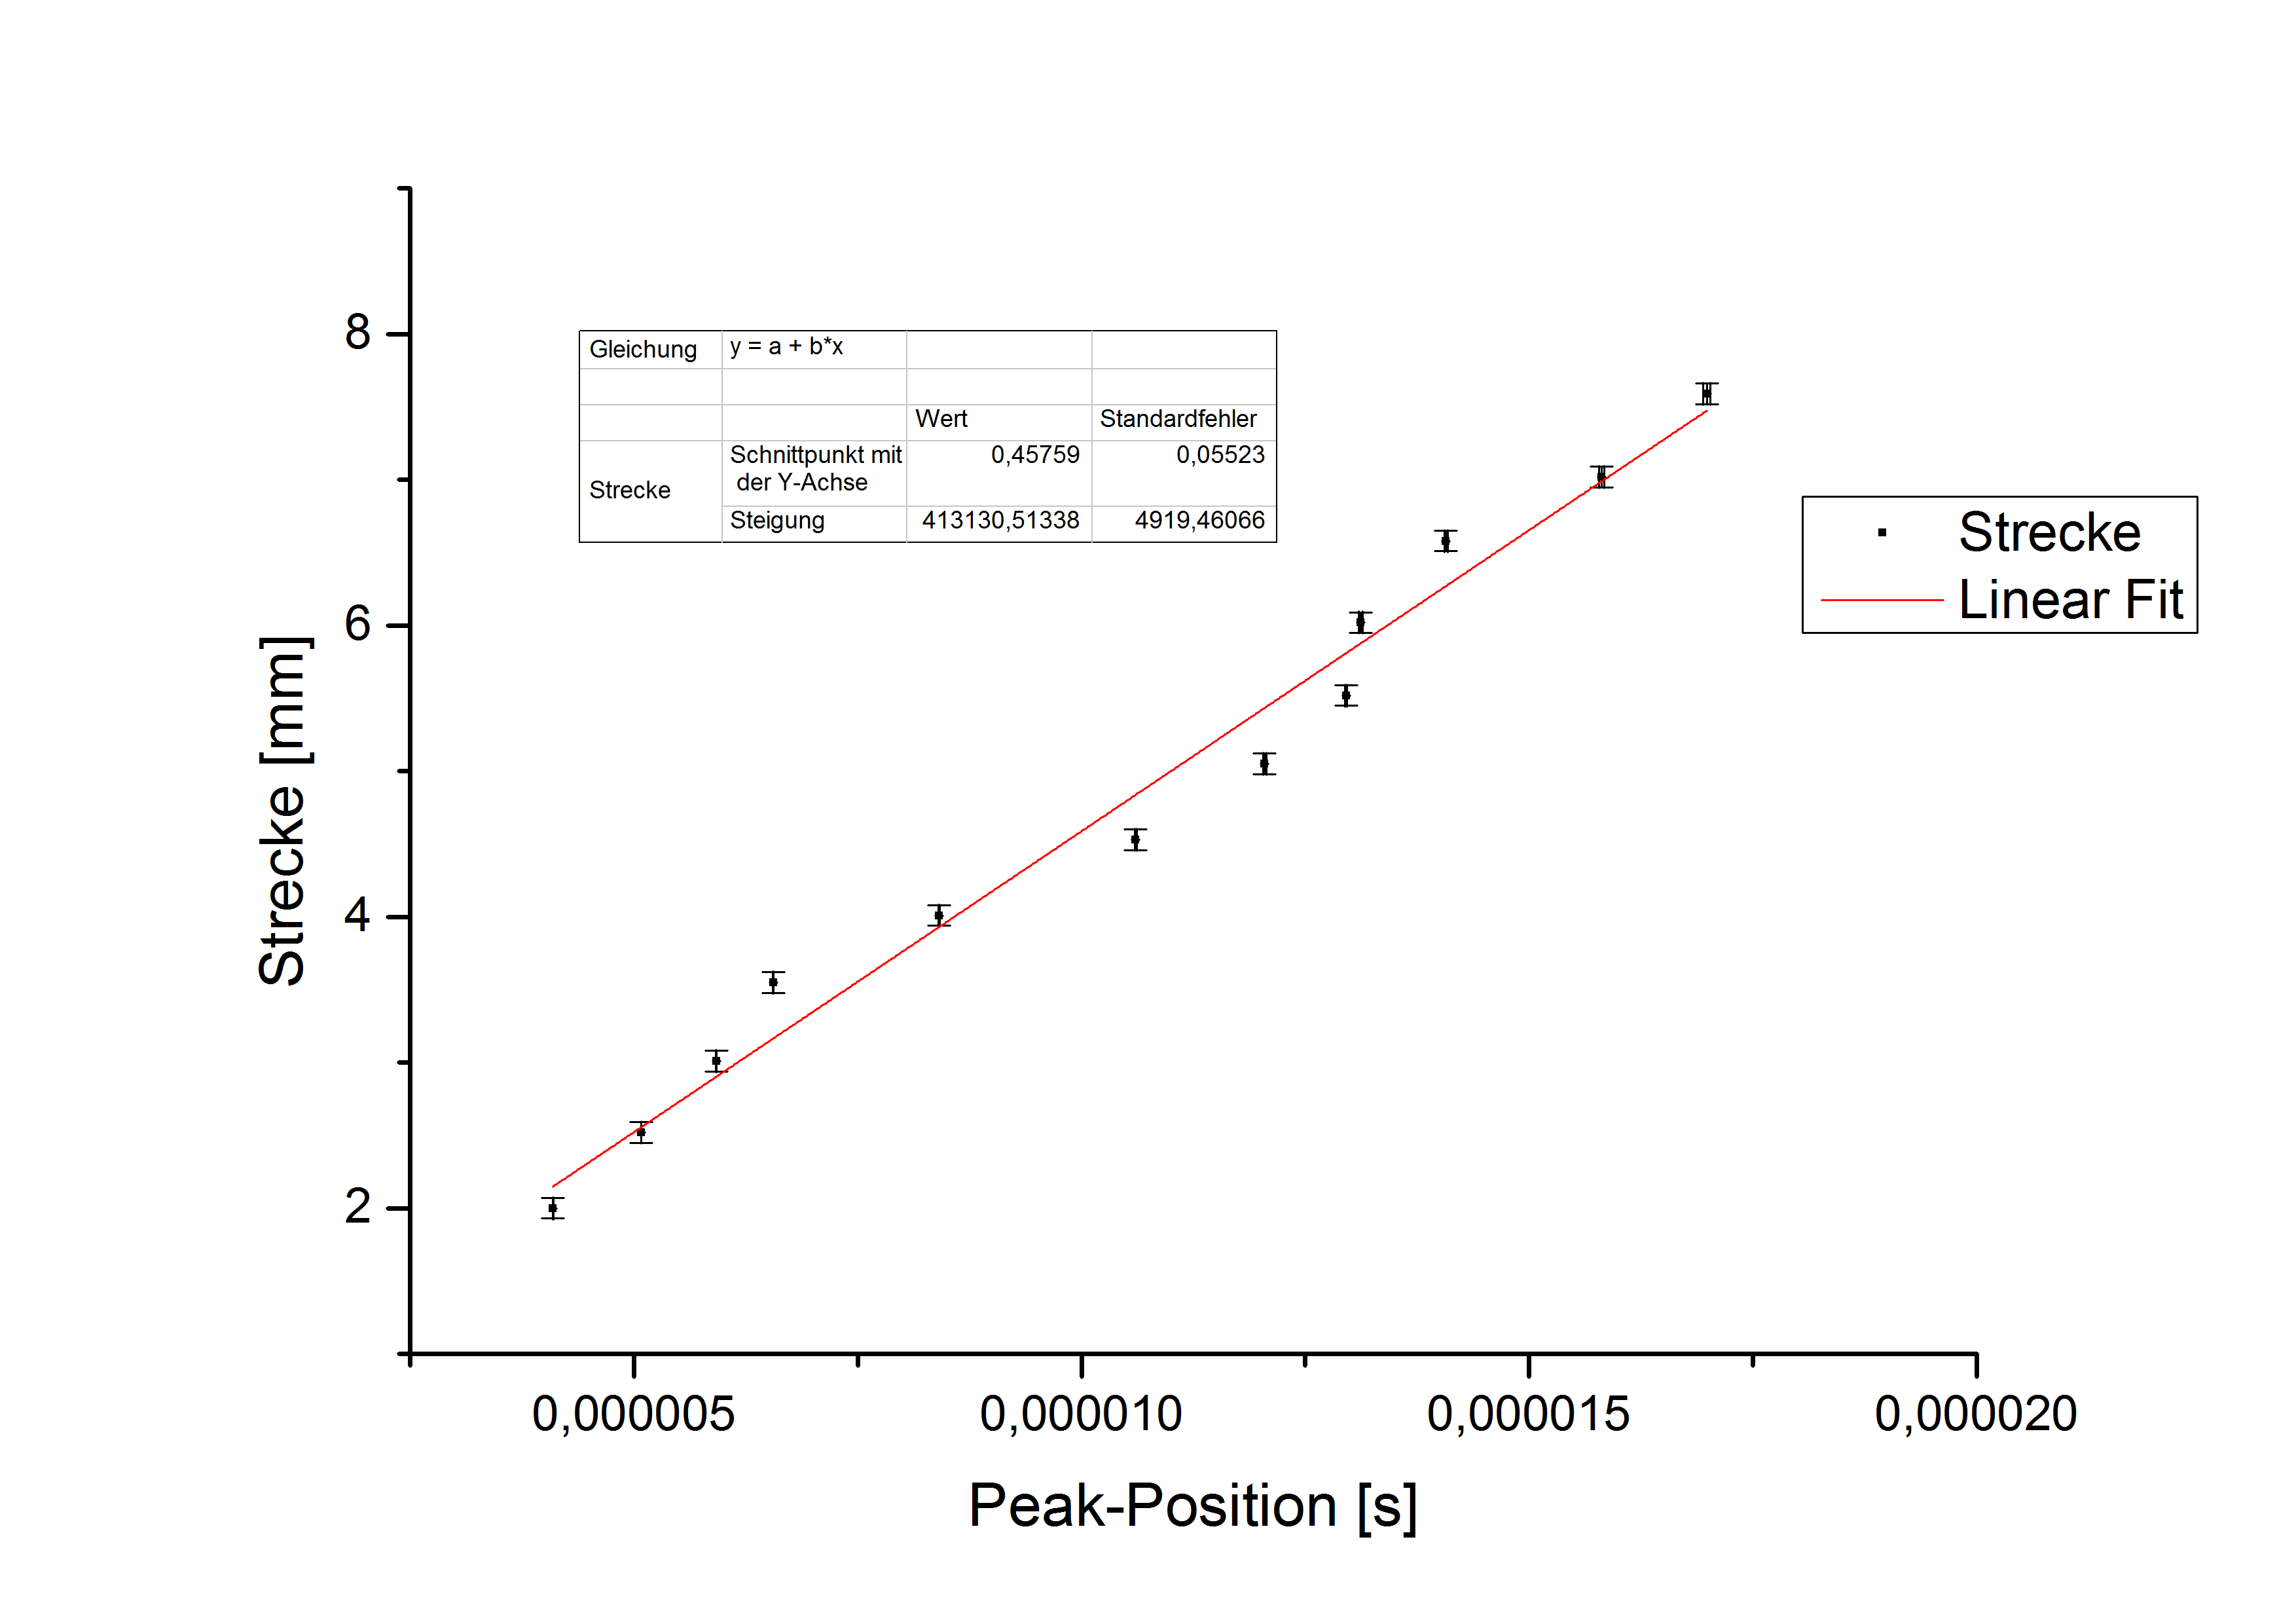
\includegraphics[scale=0.5]{Bilder/t2_1_my}
\caption{Linear relation of the distance to $\mathit{\mu_{n}}$. }
\label{fig:1my}
\end{center}
\end{figure}
The electric field $\mathit{E=(1.70\pm0.04)\frac{V}{mm}}$. It is easy to see that out $\mathit{x_{c}(t)=\mu_{n}Et}$ the $\mathit{\mu_{n}E}$ corresponds to the pitch $\mathit{b}$, so $\mathit{\mu_{n}=b/E}$ and $\mathit{s_{\mu_{n}}=\sqrt{(\frac{s_{b}}{E})^2+(-\frac{b}{E^2}s_{E})^2}}$.
\newpage
The mean lifetime $\mathit{\tau}$ is directly calculated and shown as a parameter of the fit.
\begin{figure}[h]
\begin{center}
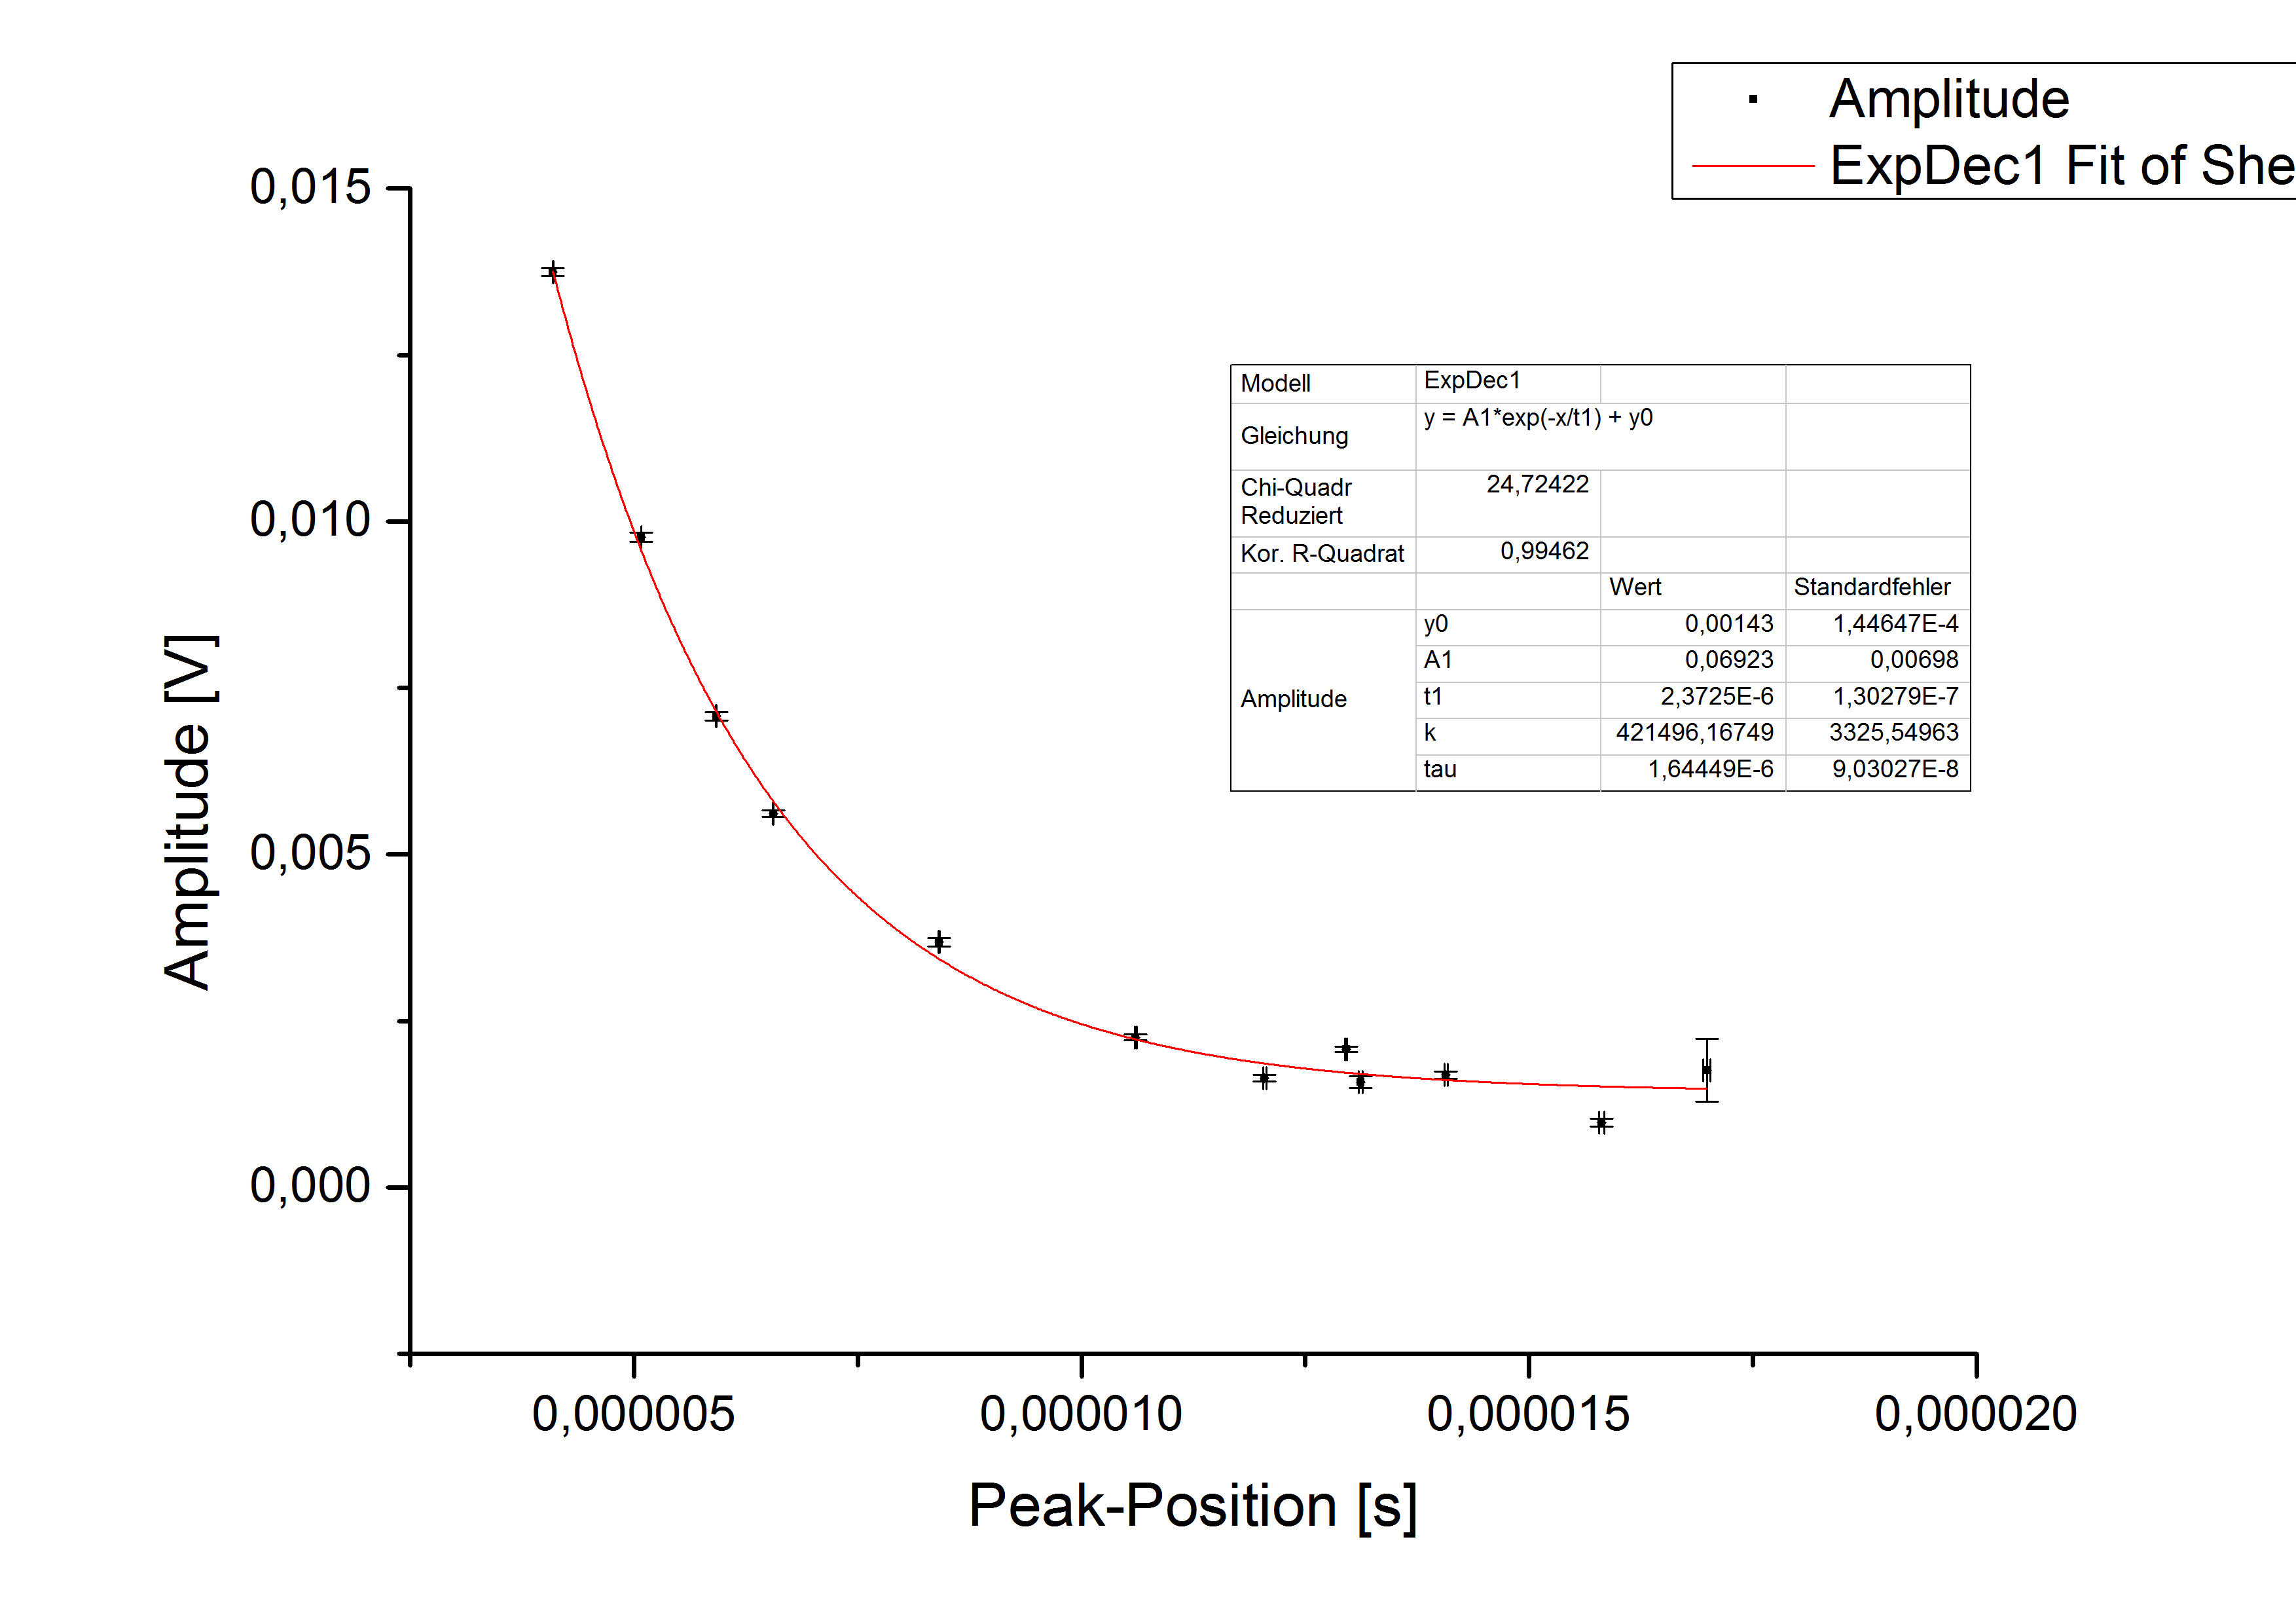
\includegraphics[scale=0.5]{Bilder/t2_1_tau}
\caption{Exponential decay as fit of the amplitude, to get $\mathit{\tau_{n}}$. }
\label{fig:1tau}
\end{center}
\end{figure}
\newpage
The square-root-function gives us the mass diffusivity $\mathit{D_{e}}$:
\begin{figure}[h]
\begin{center}
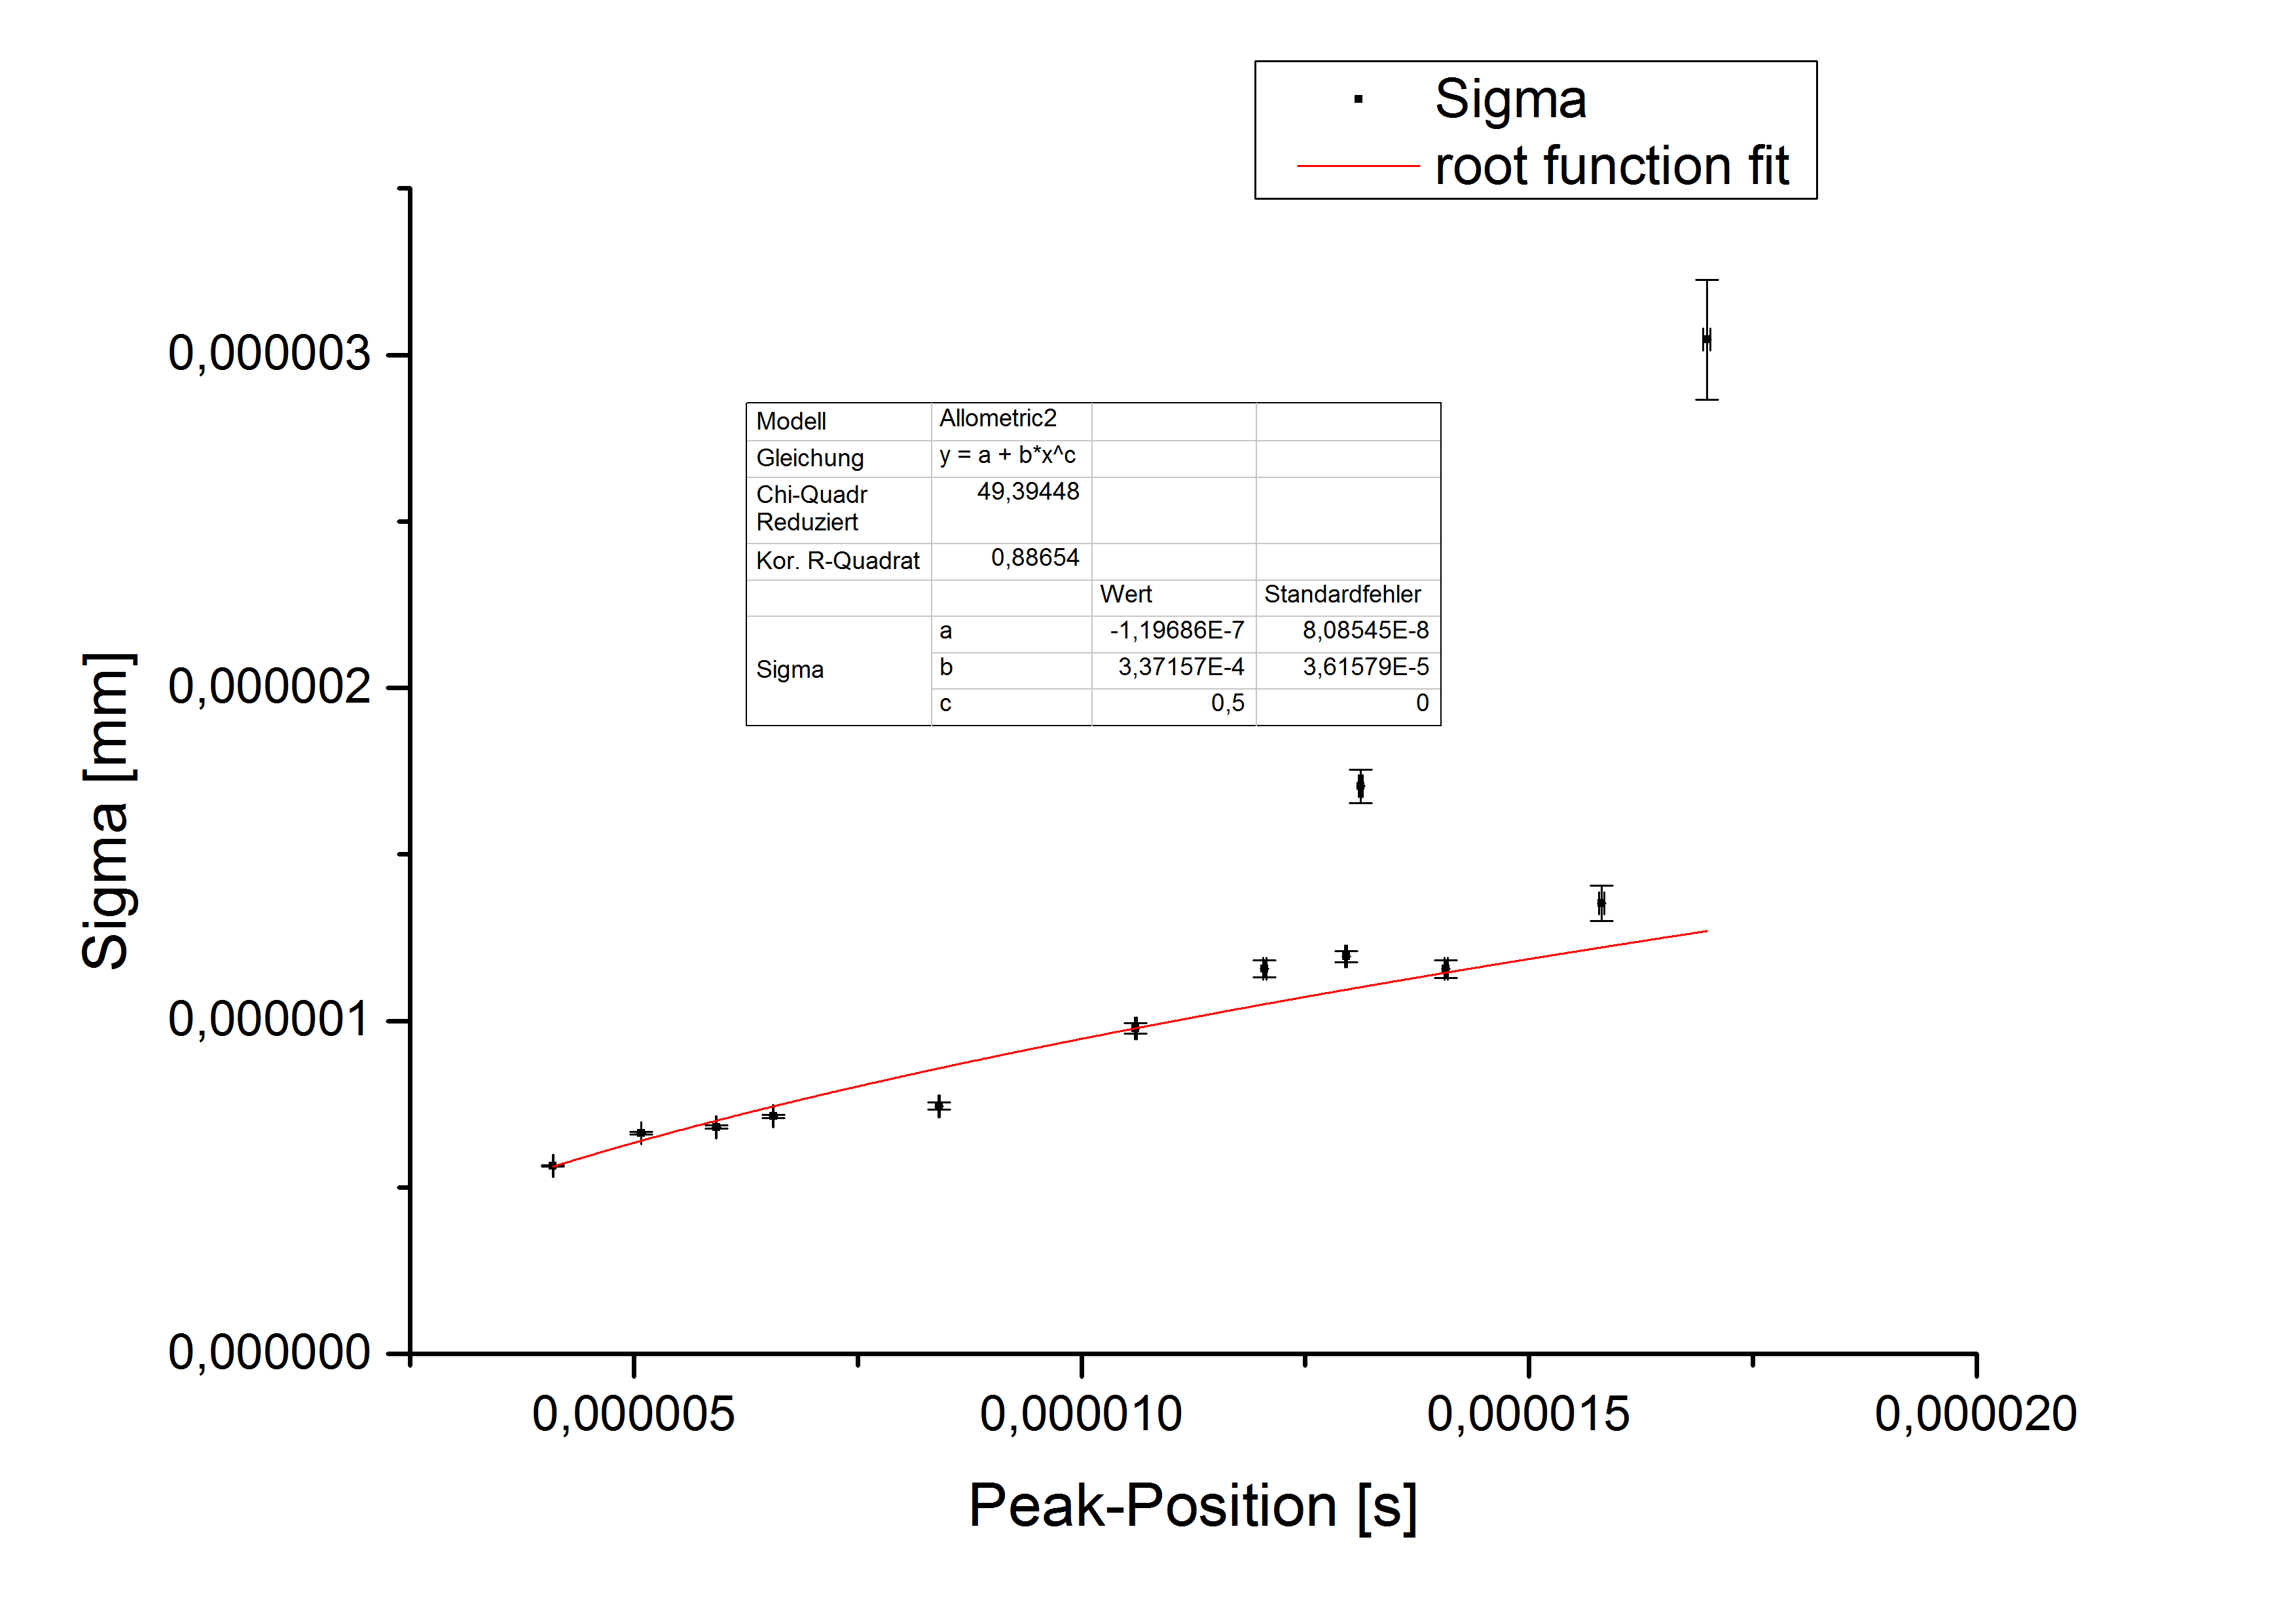
\includegraphics[scale=0.5]{Bilder/t2_1_sigma}
\caption{Square root function as fit of the sigma, to get $\mathit{D_{e}}$. }
\label{fig:1sigma}
\end{center}
\end{figure}\\
Easy to see that $\mathit{b^2= 2 D_{e}}$, so we get:\\
$\mathit{D_{e}=\frac{b^2}{2}}$ and \\
$\mathit{s_{D_{e}}=b\cdot s_{b}}$.\\
\\
So our results from the first series of measurements is:\\

$\mathit{\mu_{n}=(2420\pm70)\frac{cm^{2}}{Vs}}$\\

$\mathit{\tau_{n}=(2.4\pm0.1)\cdot10^{-6}s}$\\

$\mathit{D_{e}=(5\pm1)\cdot10^{-8}\frac{mm^{2}}{s}}$
\newpage
\subsection*{2. Measurements}
At the variation of the charge, we had $\mathit{x_{c}(t)=\mu_{n}\frac{U}{l}t}$ an form it to $\mathit{U(t)=\frac{x_{c} \cdot l}{\mu_{n}}\frac{1}{t}}$, at which $\mathit{x_{c}(t)=const}$ an $\mathit{l}$ is the length of the Ge-pad. The $\mathit{1/x}$-function fit gives us:\\
\begin{figure}[h]
\begin{center}
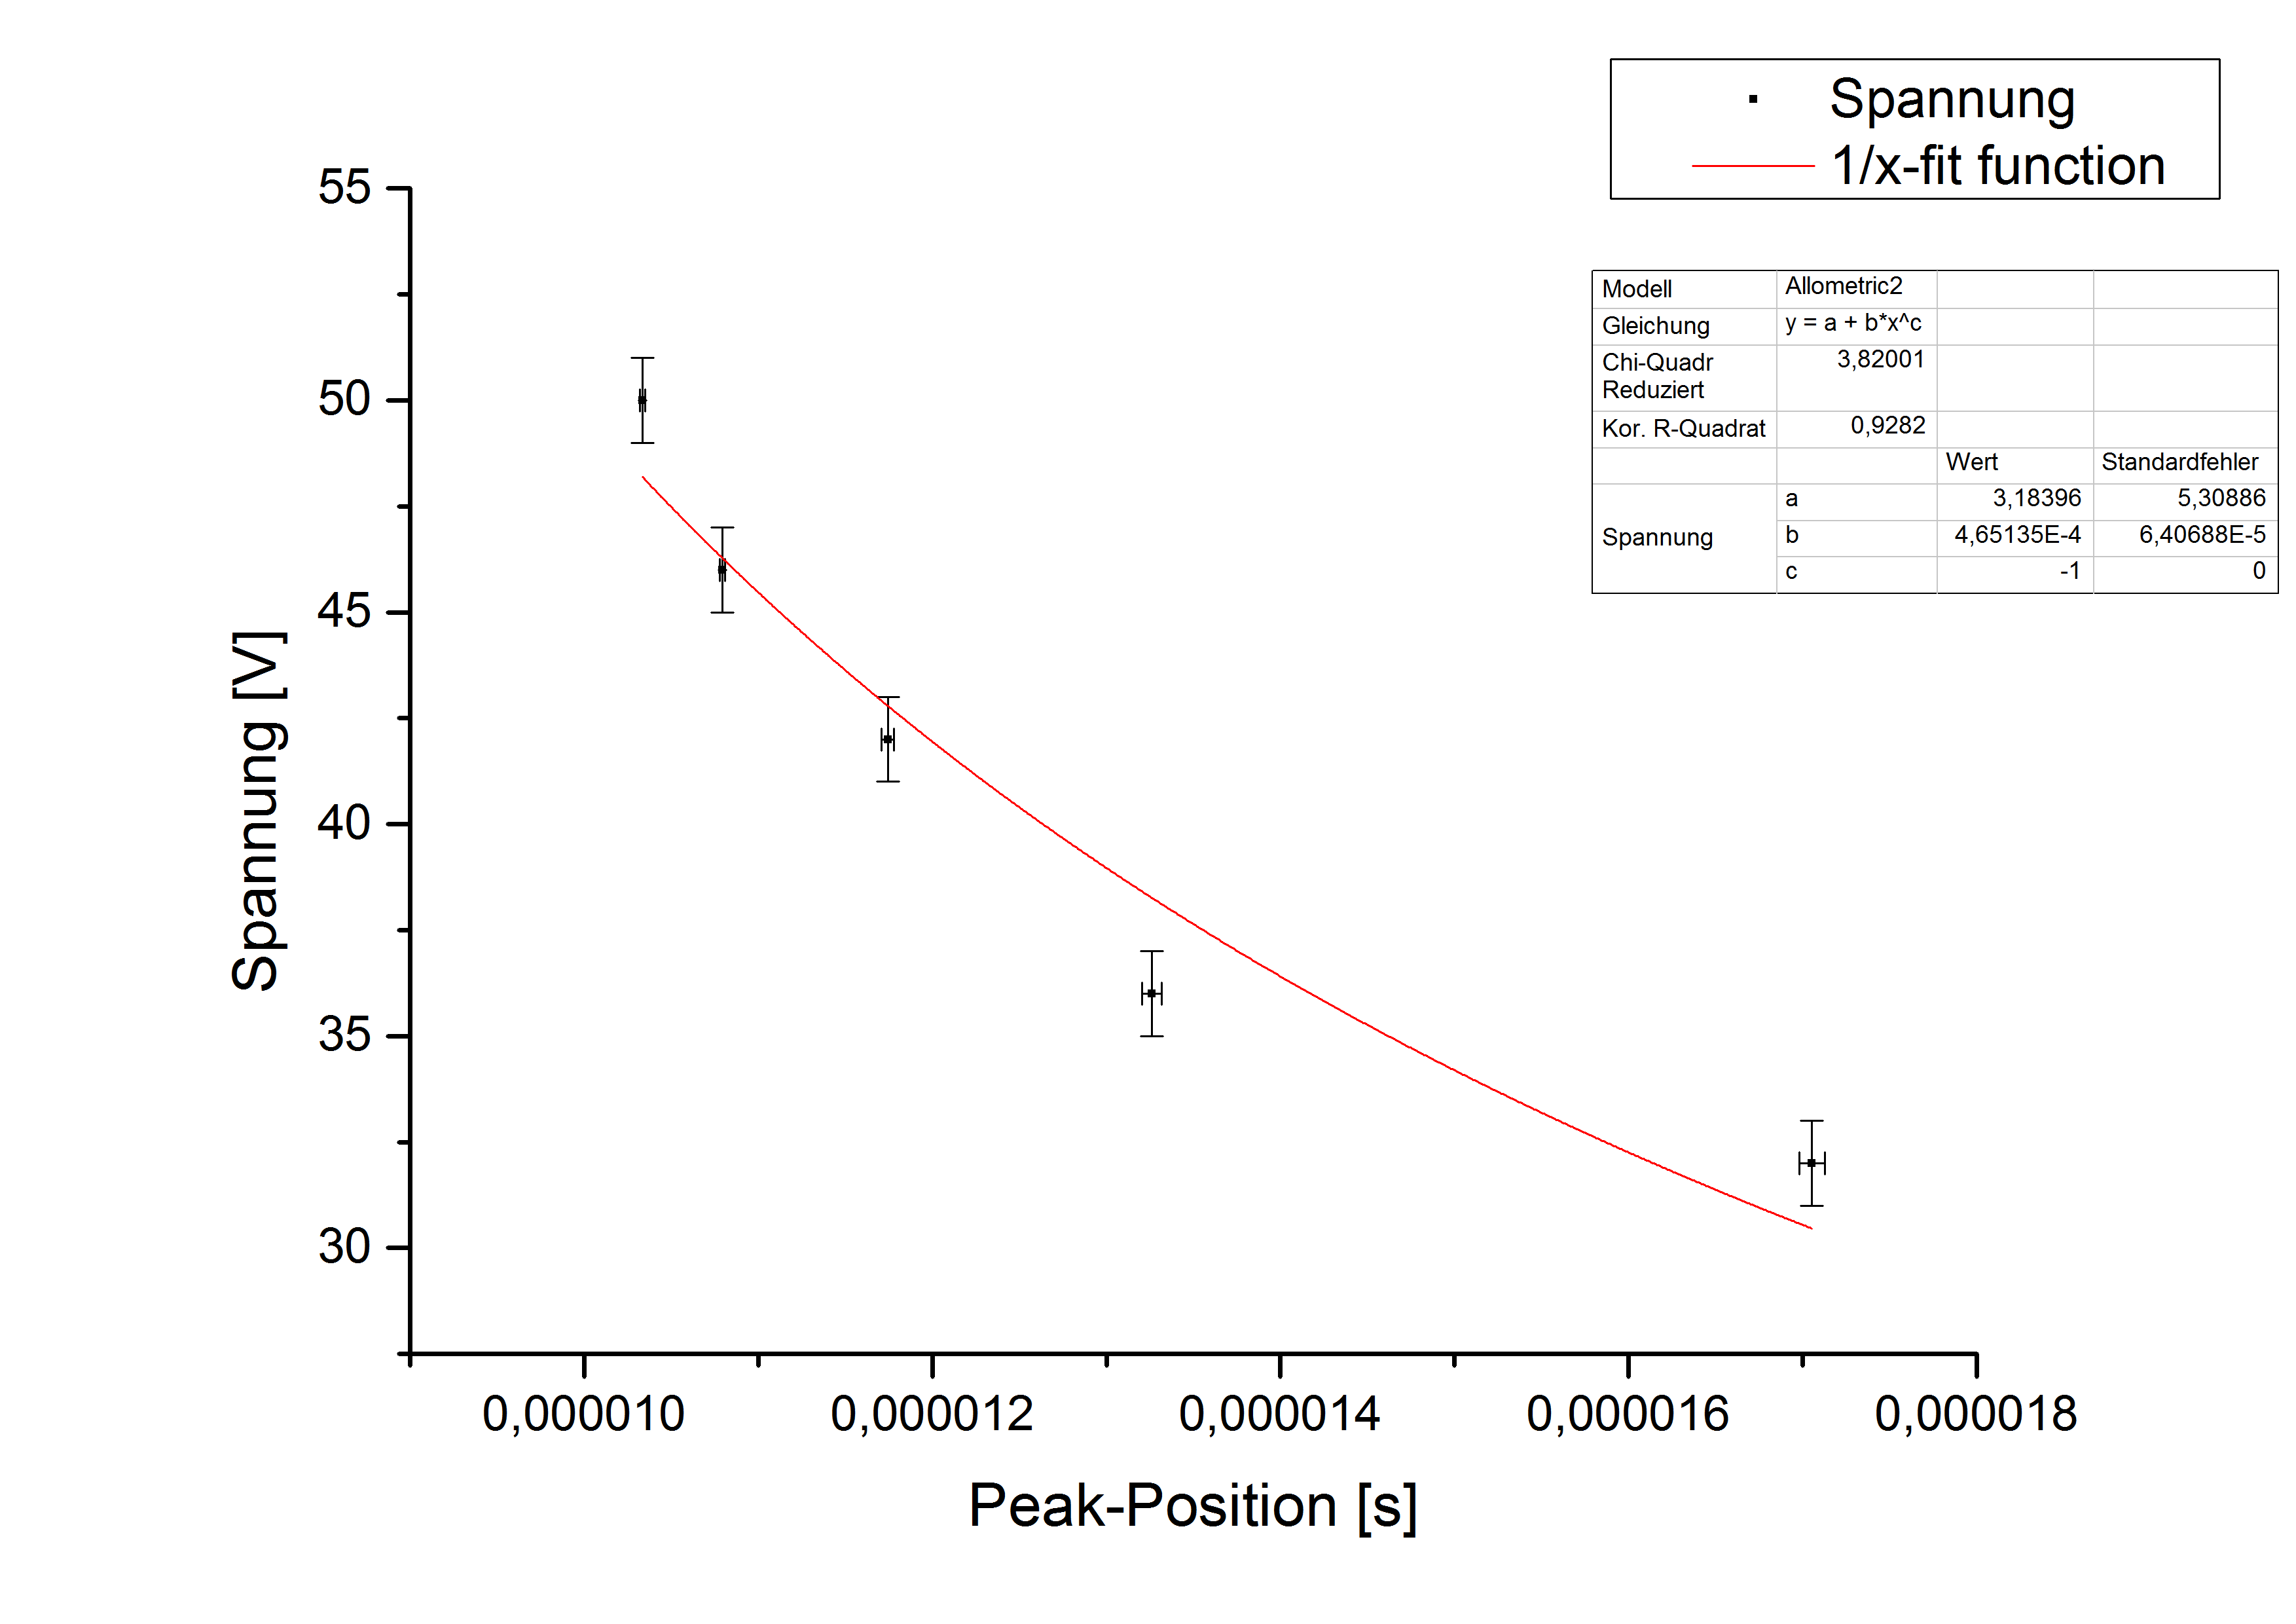
\includegraphics[scale=0.5]{Bilder/t2_2_my}
\caption{$\mathit{1/x}$-function fit of the voltage, to get $\mathit{\mu_{n}}$. }
\label{fig:2my}
\end{center}
\end{figure}\\
With the parameter $\mathit{b}$ is $\mathit{\mu_{n}=\frac{x_{c} \cdot l}{b}}$ and $\mathit{s_{\mu_{n}}=\sqrt{(\frac{l}{b}\cdot s_{x_{c}})^2+(\frac{x_{c}}{b}\cdot s_{l})^2+(\frac{x_{c} \cdot l}{b^2}\cdot s_{b})^2}}$ we can calculate $\mathit{\mu_{n}}$.
\newpage
$\mathit{\tau}$ can be read out of the fit parameters.
\begin{figure}[h]
\begin{center}
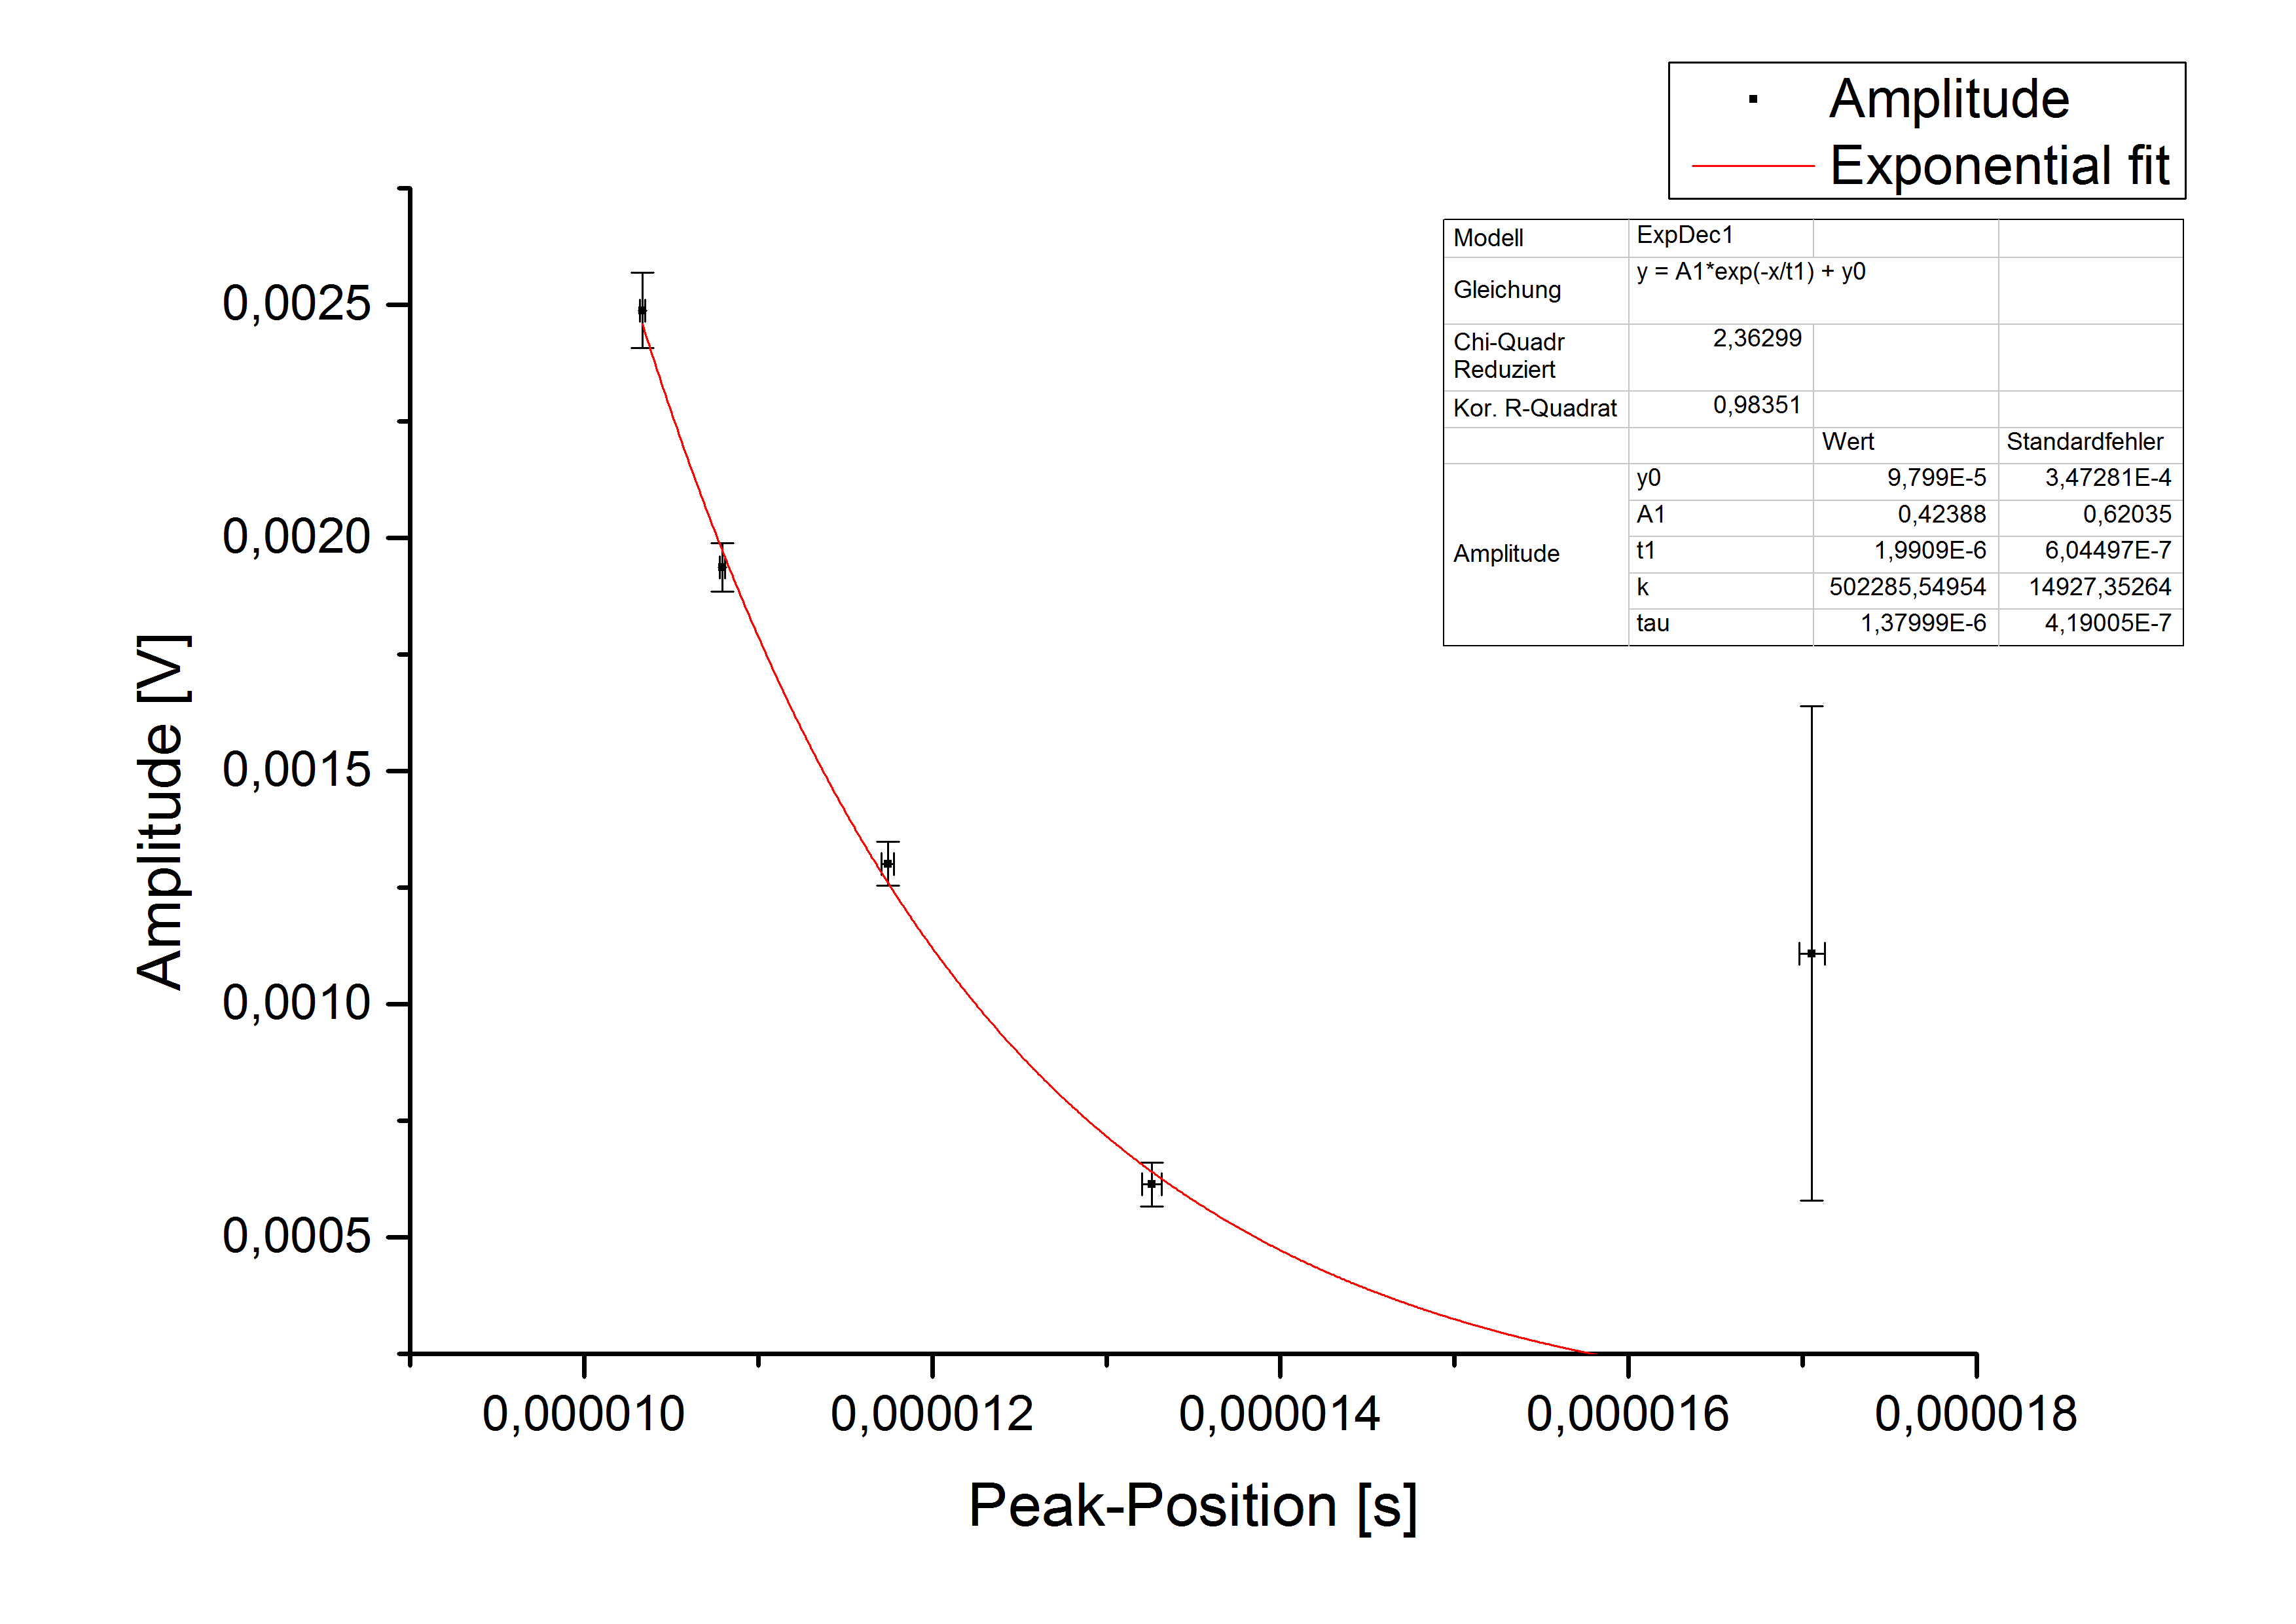
\includegraphics[scale=0.5]{Bilder/t2_2_tau}
\caption{Exponential decay fit of the amplitude, to get $\mathit{\tau}$. }
\label{fig:2tau}
\end{center}
\end{figure}\\
\newpage
The calculation of $\mathit{D_{n}}$ works the same way as in the first series.
\begin{figure}[h]
\begin{center}
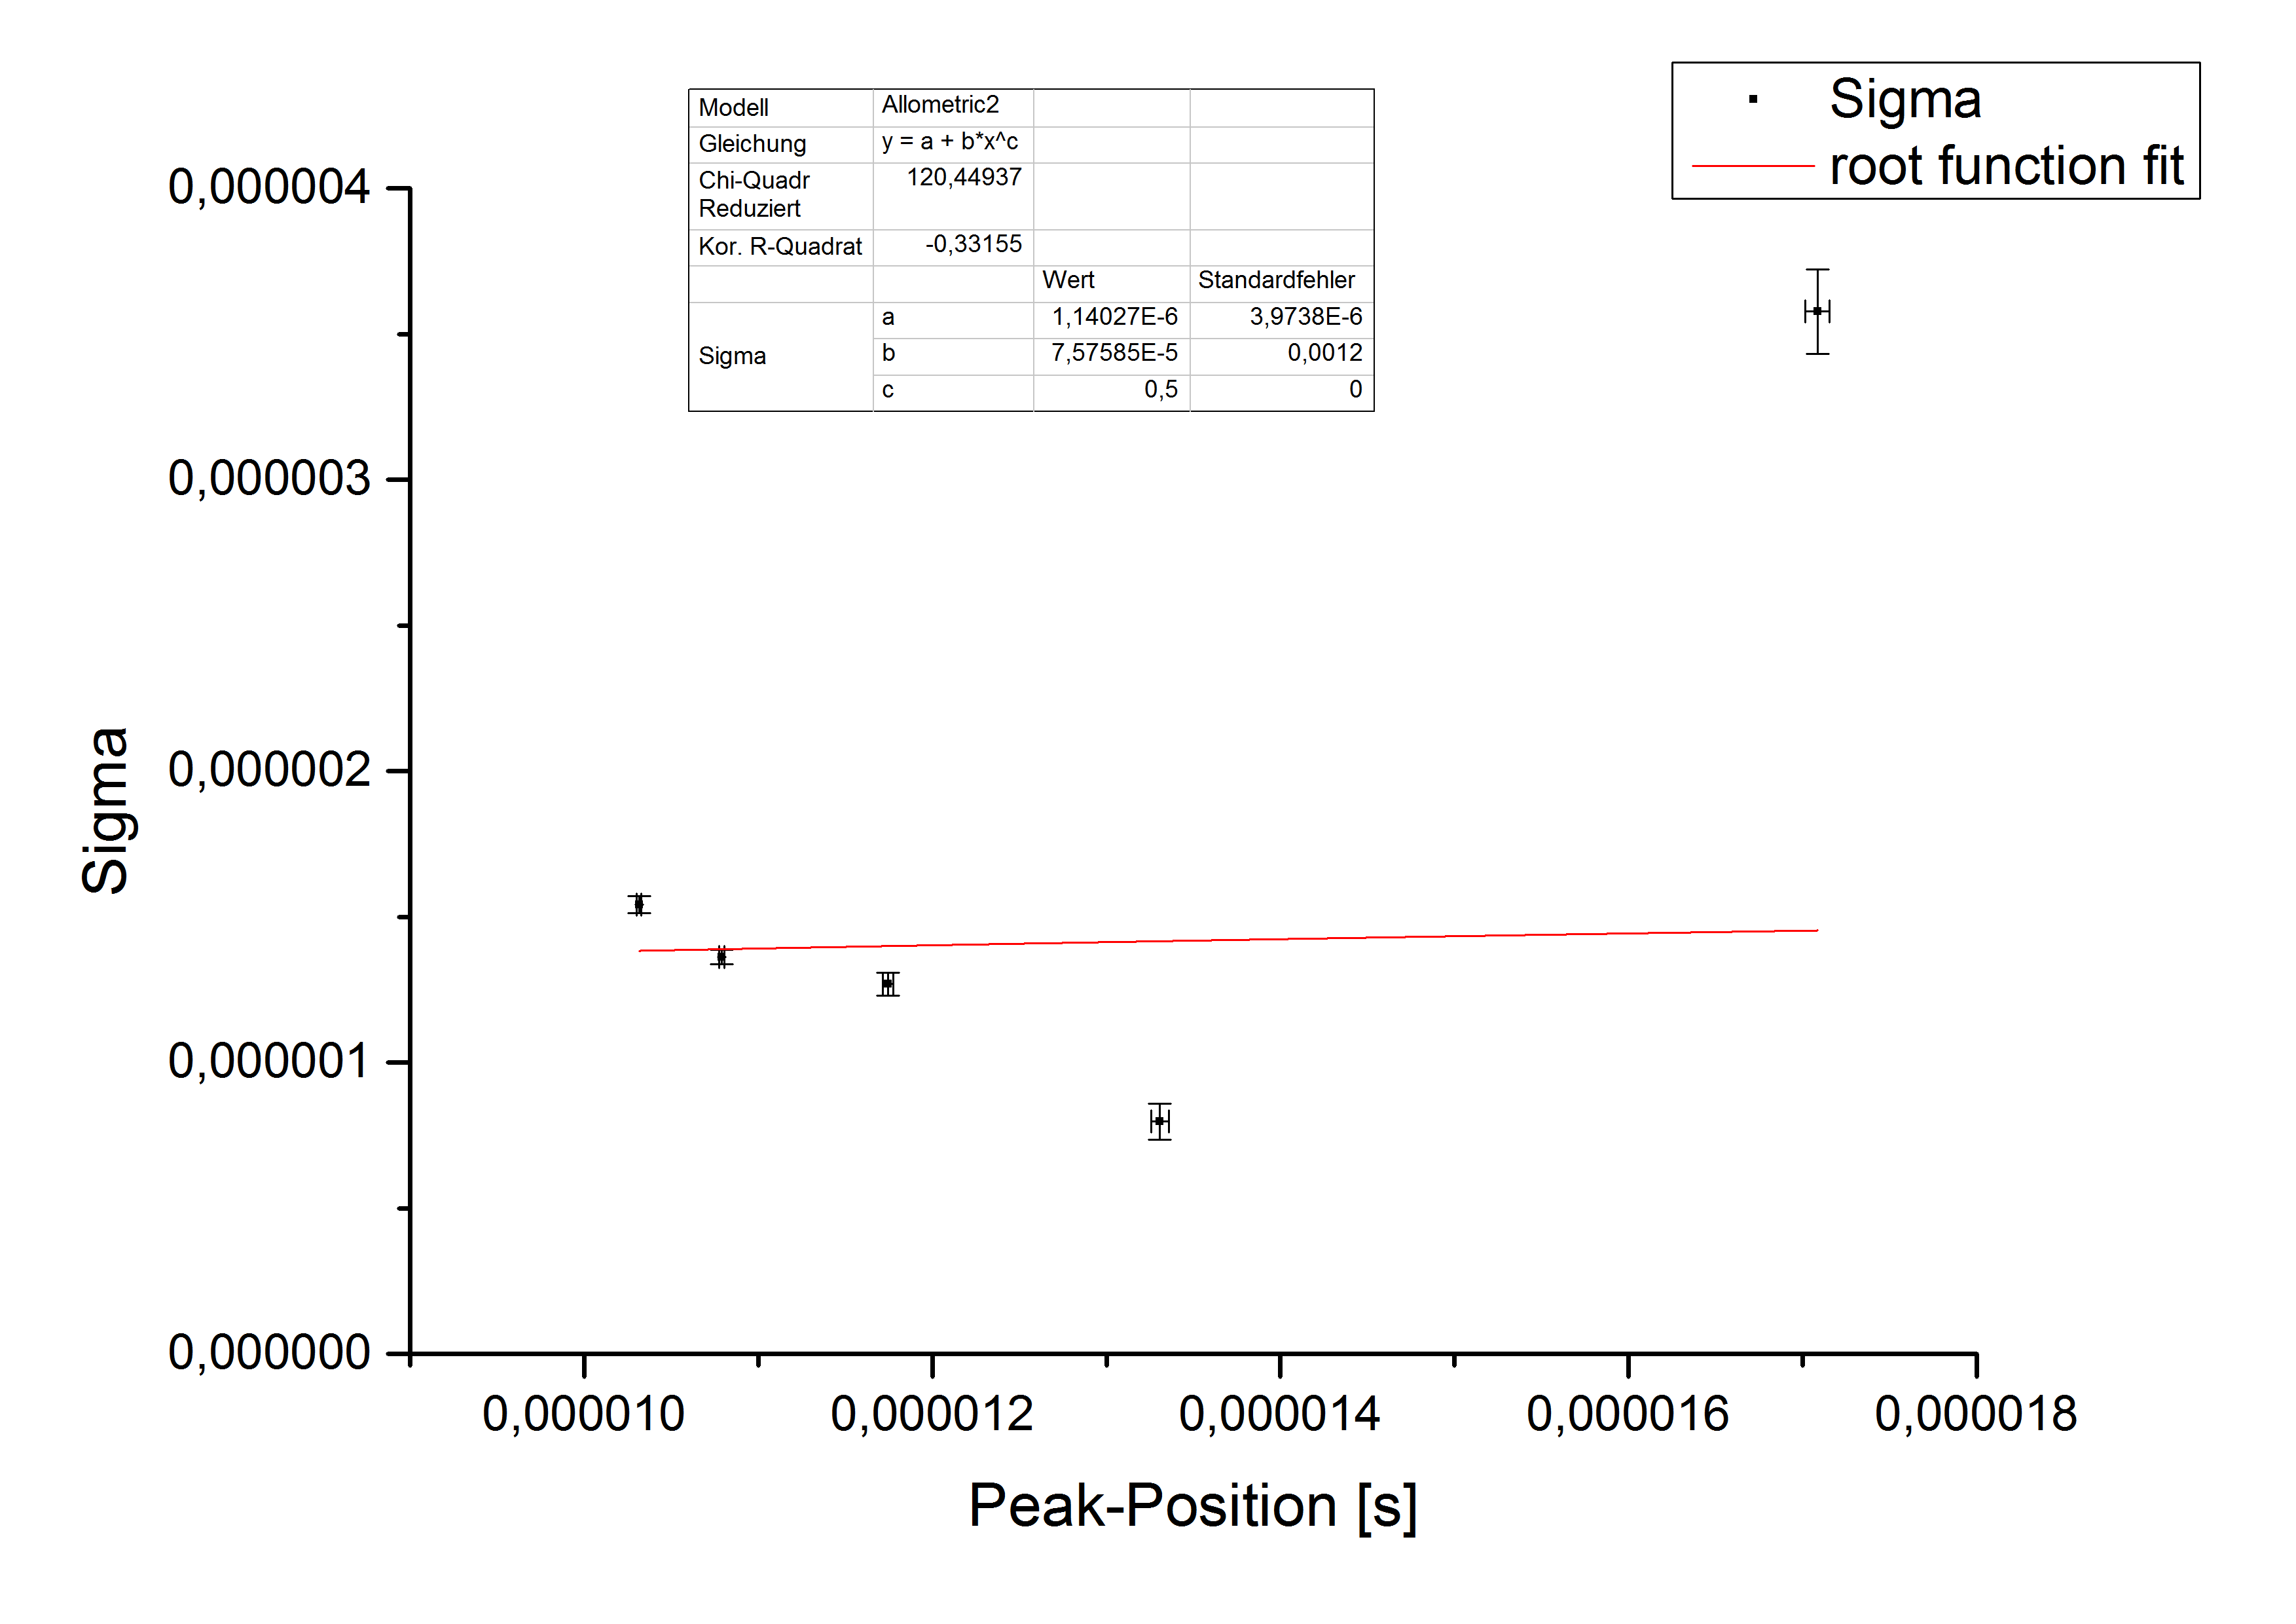
\includegraphics[scale=0.5]{Bilder/t2_2_sigma}
\caption{Exponential decay fit of the amplitude, to get $\mathit{\tau}$. }
\label{fig:2sigma}
\end{center}
\end{figure}\\
So our results from the second series of measurements is:\\

$\mathit{\mu_{n}=(2600\pm400)\frac{cm^{2}}{Vs}}$\\

$\mathit{\tau_{n}=(2.0\pm0.6)\cdot10^{-6}s}$\\

$\mathit{D_{e}=(0.3\pm9.1)\cdot10^{-8}\frac{mm^{2}}{s}}$

The literature values are the following:\\
\begin{center}
Mobility $\mu=3900 \frac{cm^2}{Vs}$\\
Mean lifetime $\tau=(45\pm 2)*10^{-6} s$\\
Diffusion constant $D_{n}=101 \frac{cm^2}{s}$
\end{center}
~\\
$\mu$ is in the same dimension of magnitude as the literature value. For $\tau$ and $D_{n}$, our results are far from their respective literature values. A possible explanation for this might be a contamination of the Ge-sample. Also, we did not take into account the errors on the oscilloscope. Still, we do not think these errors are what caused our bad results. As especially in the 2nd part of the experiment the signal decreased its width instead of increasing it, there has to be an issue about the oscilloscope causing a systematic error. 
\chapter{Experiment No.3: Semiconductor Detectors}
\section{Description}
\textbf{ExperimentalSetup}
In this part of the experiment we connect semiconductor detectors to a Multi Channel Analyzer (MCA). The signal gets amplified as can be seen in the sketch below:\\
\begin{figure}[h]
\begin{center}
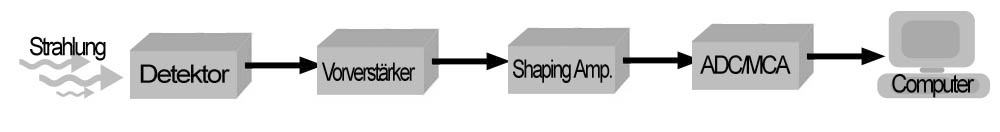
\includegraphics[scale=0.3]{Bilder/Aufbau_V3.png}\caption{Experimental setup. Source: [Ver]}\label{Halbleiterdetektor}
\end{center}
\end{figure}\\
\\
The computer measures the spectra with the help of a program called ADC. We use two different semiconductor detectors: a n-$n^{+}$-silicon-diode and a CdTe-crystal.\\
\\
\large\textbf{Signal curve}
The semiconductor detectors generate a current proportional to the energy of the incoming $\gamma-quanta$. The preamplifier boosts the signal strength. The signal then reaches the shaping amplifier, where it charges a capacitor, which gets discharged with the help of an electric resistance (CR-filter). The signal has to cross two RC-filters afterwards, which damp the increase of the resulting signal. This $CR-(RC)^2-shaping$ creates a voltage peak. The proportionality between the incoming photon energy and the peak is maintained.\\
\\
\section{Analysis}
The spectra of Am-241 and Co-57 with both detectors can be found in the appendix. For the 122,07 keV measured with CdTe, ADC seems to have reached the maximum counts it's capable of displaying. Thus we added the maximum count number to the counts referring to the canals where we think the peak should've been (there was a clearly visible peak, but with the wrong number of counts). Both plots are disclosed. The result looks very reasonable, so we decided to continue calculating with the corrected version. Of course a systematic error occurs this way because we don't know the exact number of maximum counts ADC is capable of displaying. But as the resulting curve looks just as expected, we decided on neglecting that error.\\
We did Gaussian fits at the following energies: 59,5 keV for Am-241, 122,07 keV and 136,47 keV for Co-57. The expectation values of the Gaussian fits allow us to connect the energies mentioned above (the peaks) to certain channel numbers. In the table below the channels referring to certain energies are listed:\\
\\
    \begin{tabular}{rrrrr}
    Detector & Sample & Channel no. & Error & Energy (keV) \\
    Si    & Am-241 & 301,8 & 0,1   & 59,5 \\
          & Co-57 & 623,7 & 0,7   & 122,06 \\
          & Co-57 & 693,9 & 0,1   & 136,47 \\
    CdTe  & Am-241 & 313,8 & 0,2   & 59,5 \\
          & Co-57 & 651,5 & 0,4   & 122,06 \\
          & Co-57 & 728,8 & 0,8   & 136,47 \\
    \end{tabular}%
  \label{tab:addlabel}%
\\
We subtracted 9 from the expectation values for CdTe as the first 9 rows in Origin were occupied with the settings. \\
Of course the channel numbers can only be integers. Still, here we decided to use the exact values with their errors as we wanted to make the energy calibrations as good as possible. The linear fits for the calibrations can be seen below:\\
\begin{figure}[h]
\begin{center}
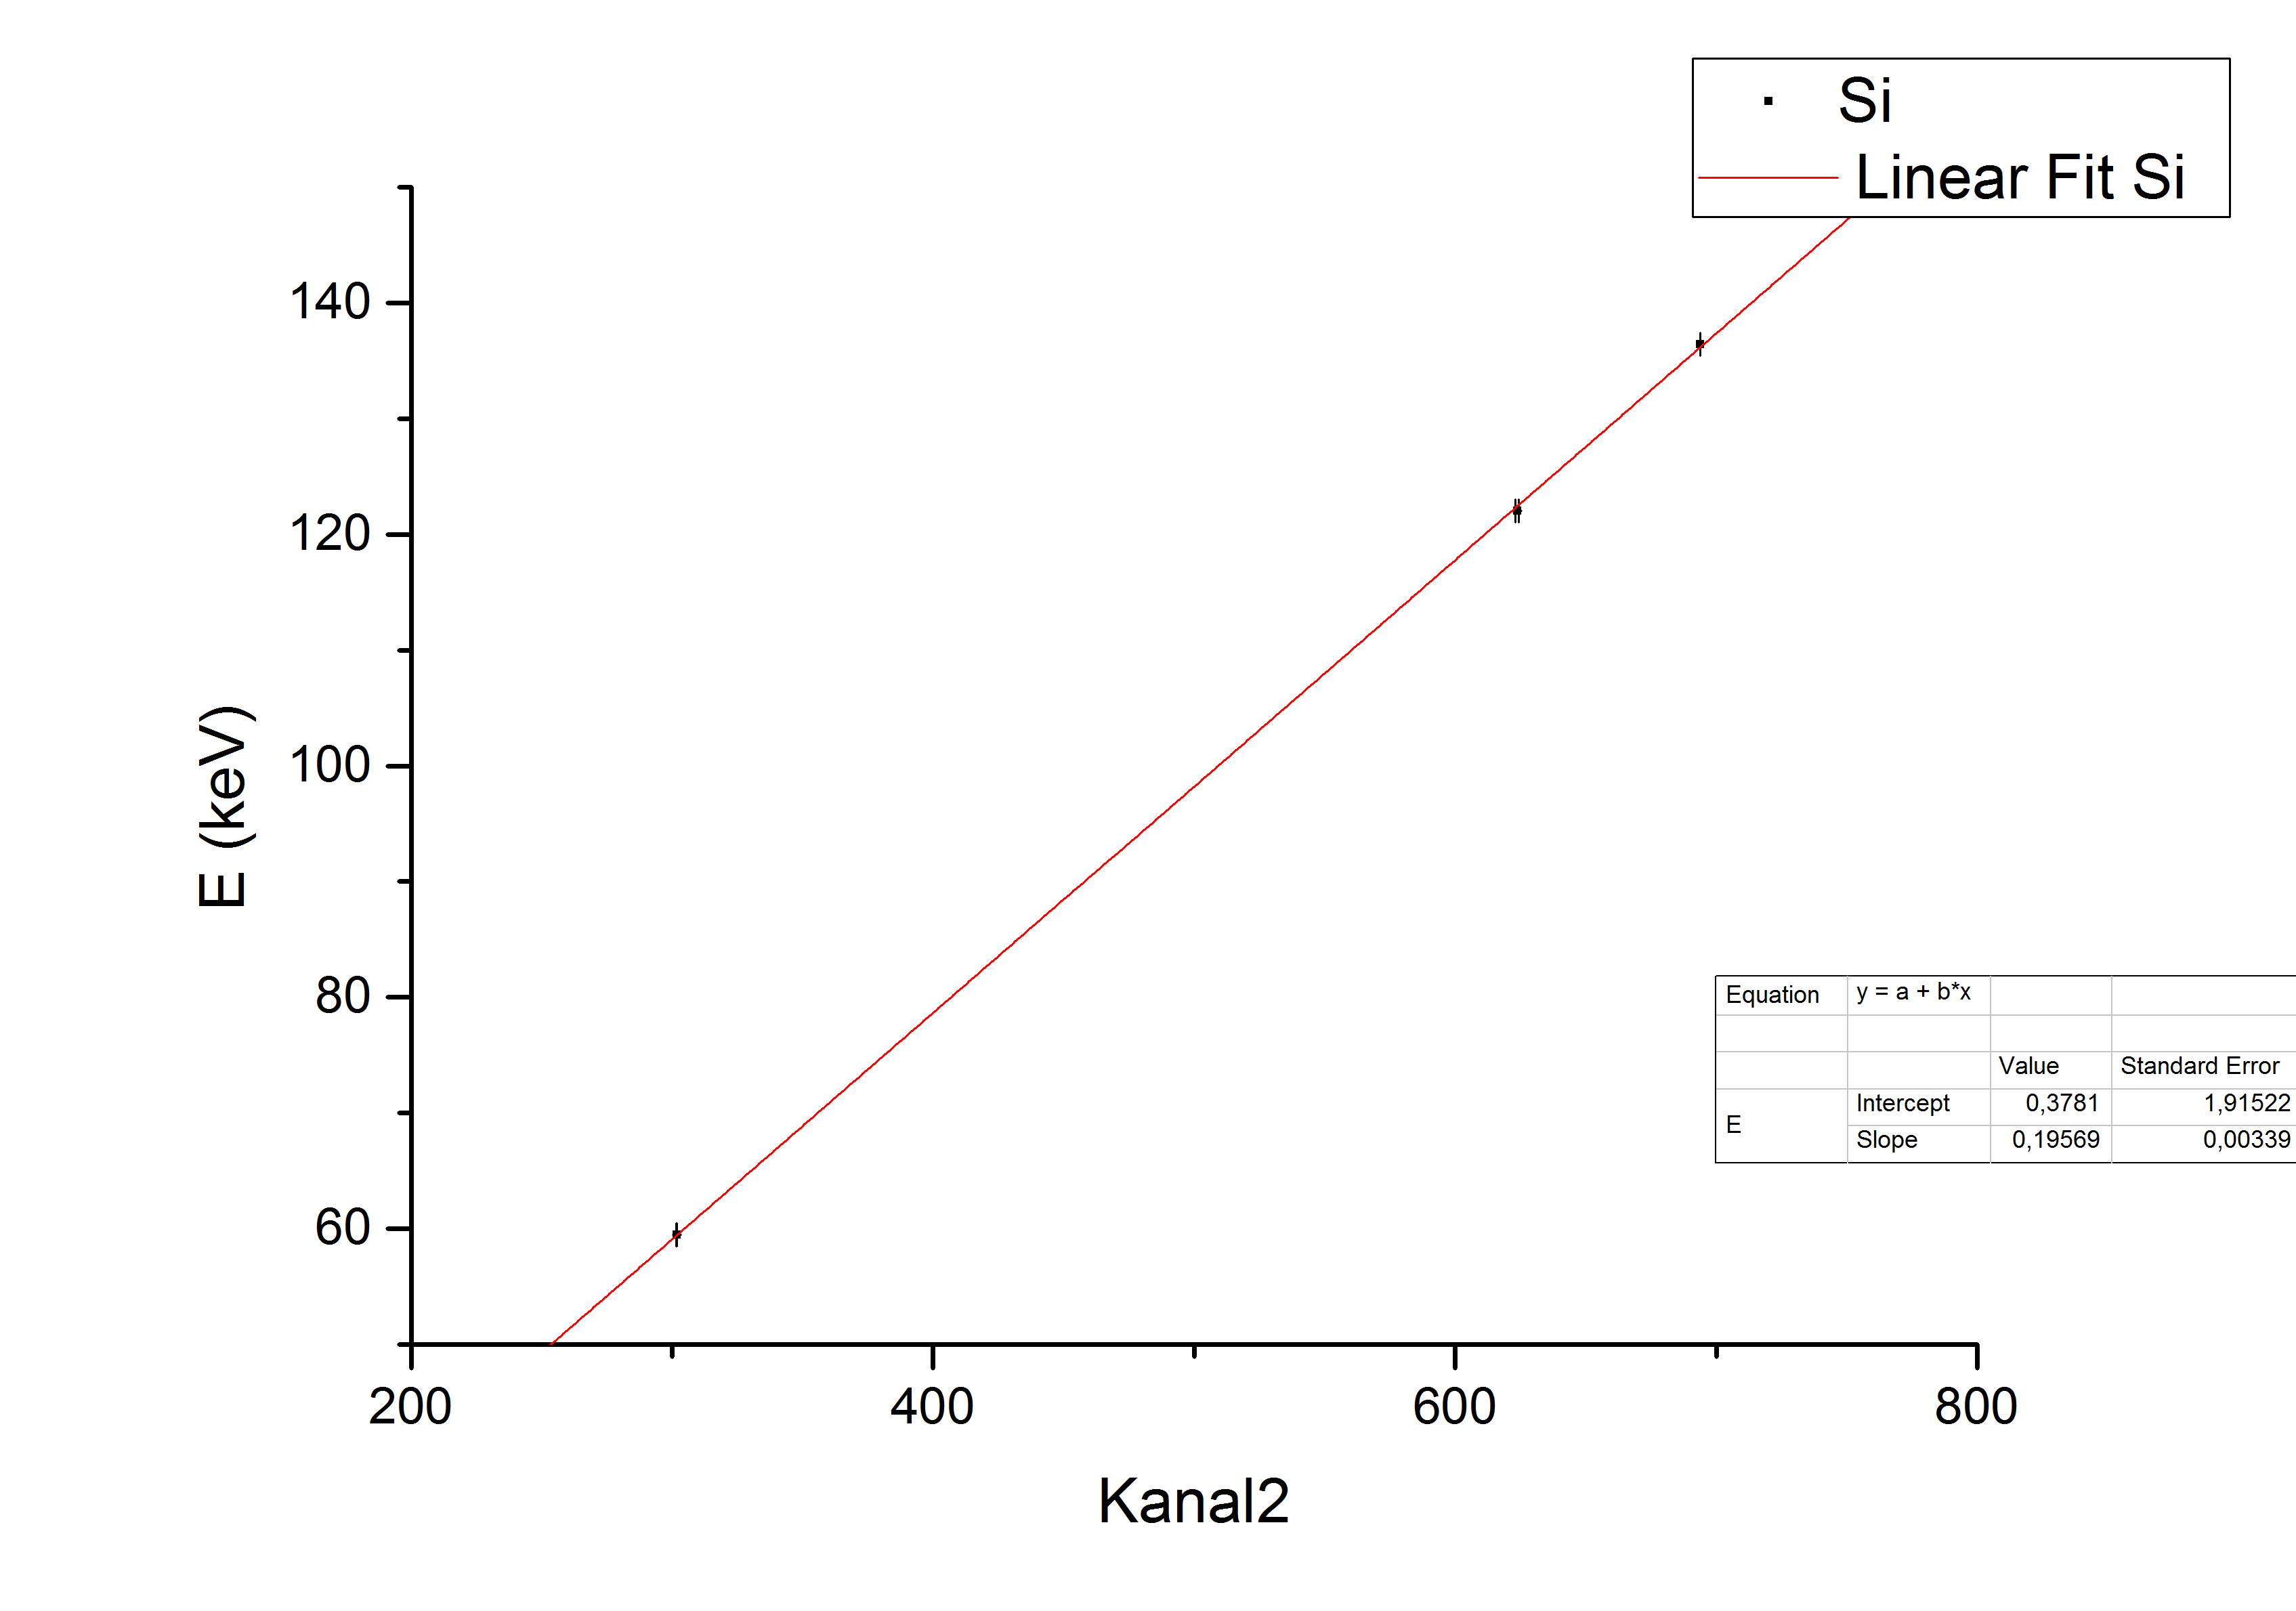
\includegraphics[scale=0.35]{Bilder/linfit_Si.png}\caption{Linear fit silicon}\label{linfit_Si}
\end{center}
\end{figure}\\
\begin{figure}[h]
\begin{center}
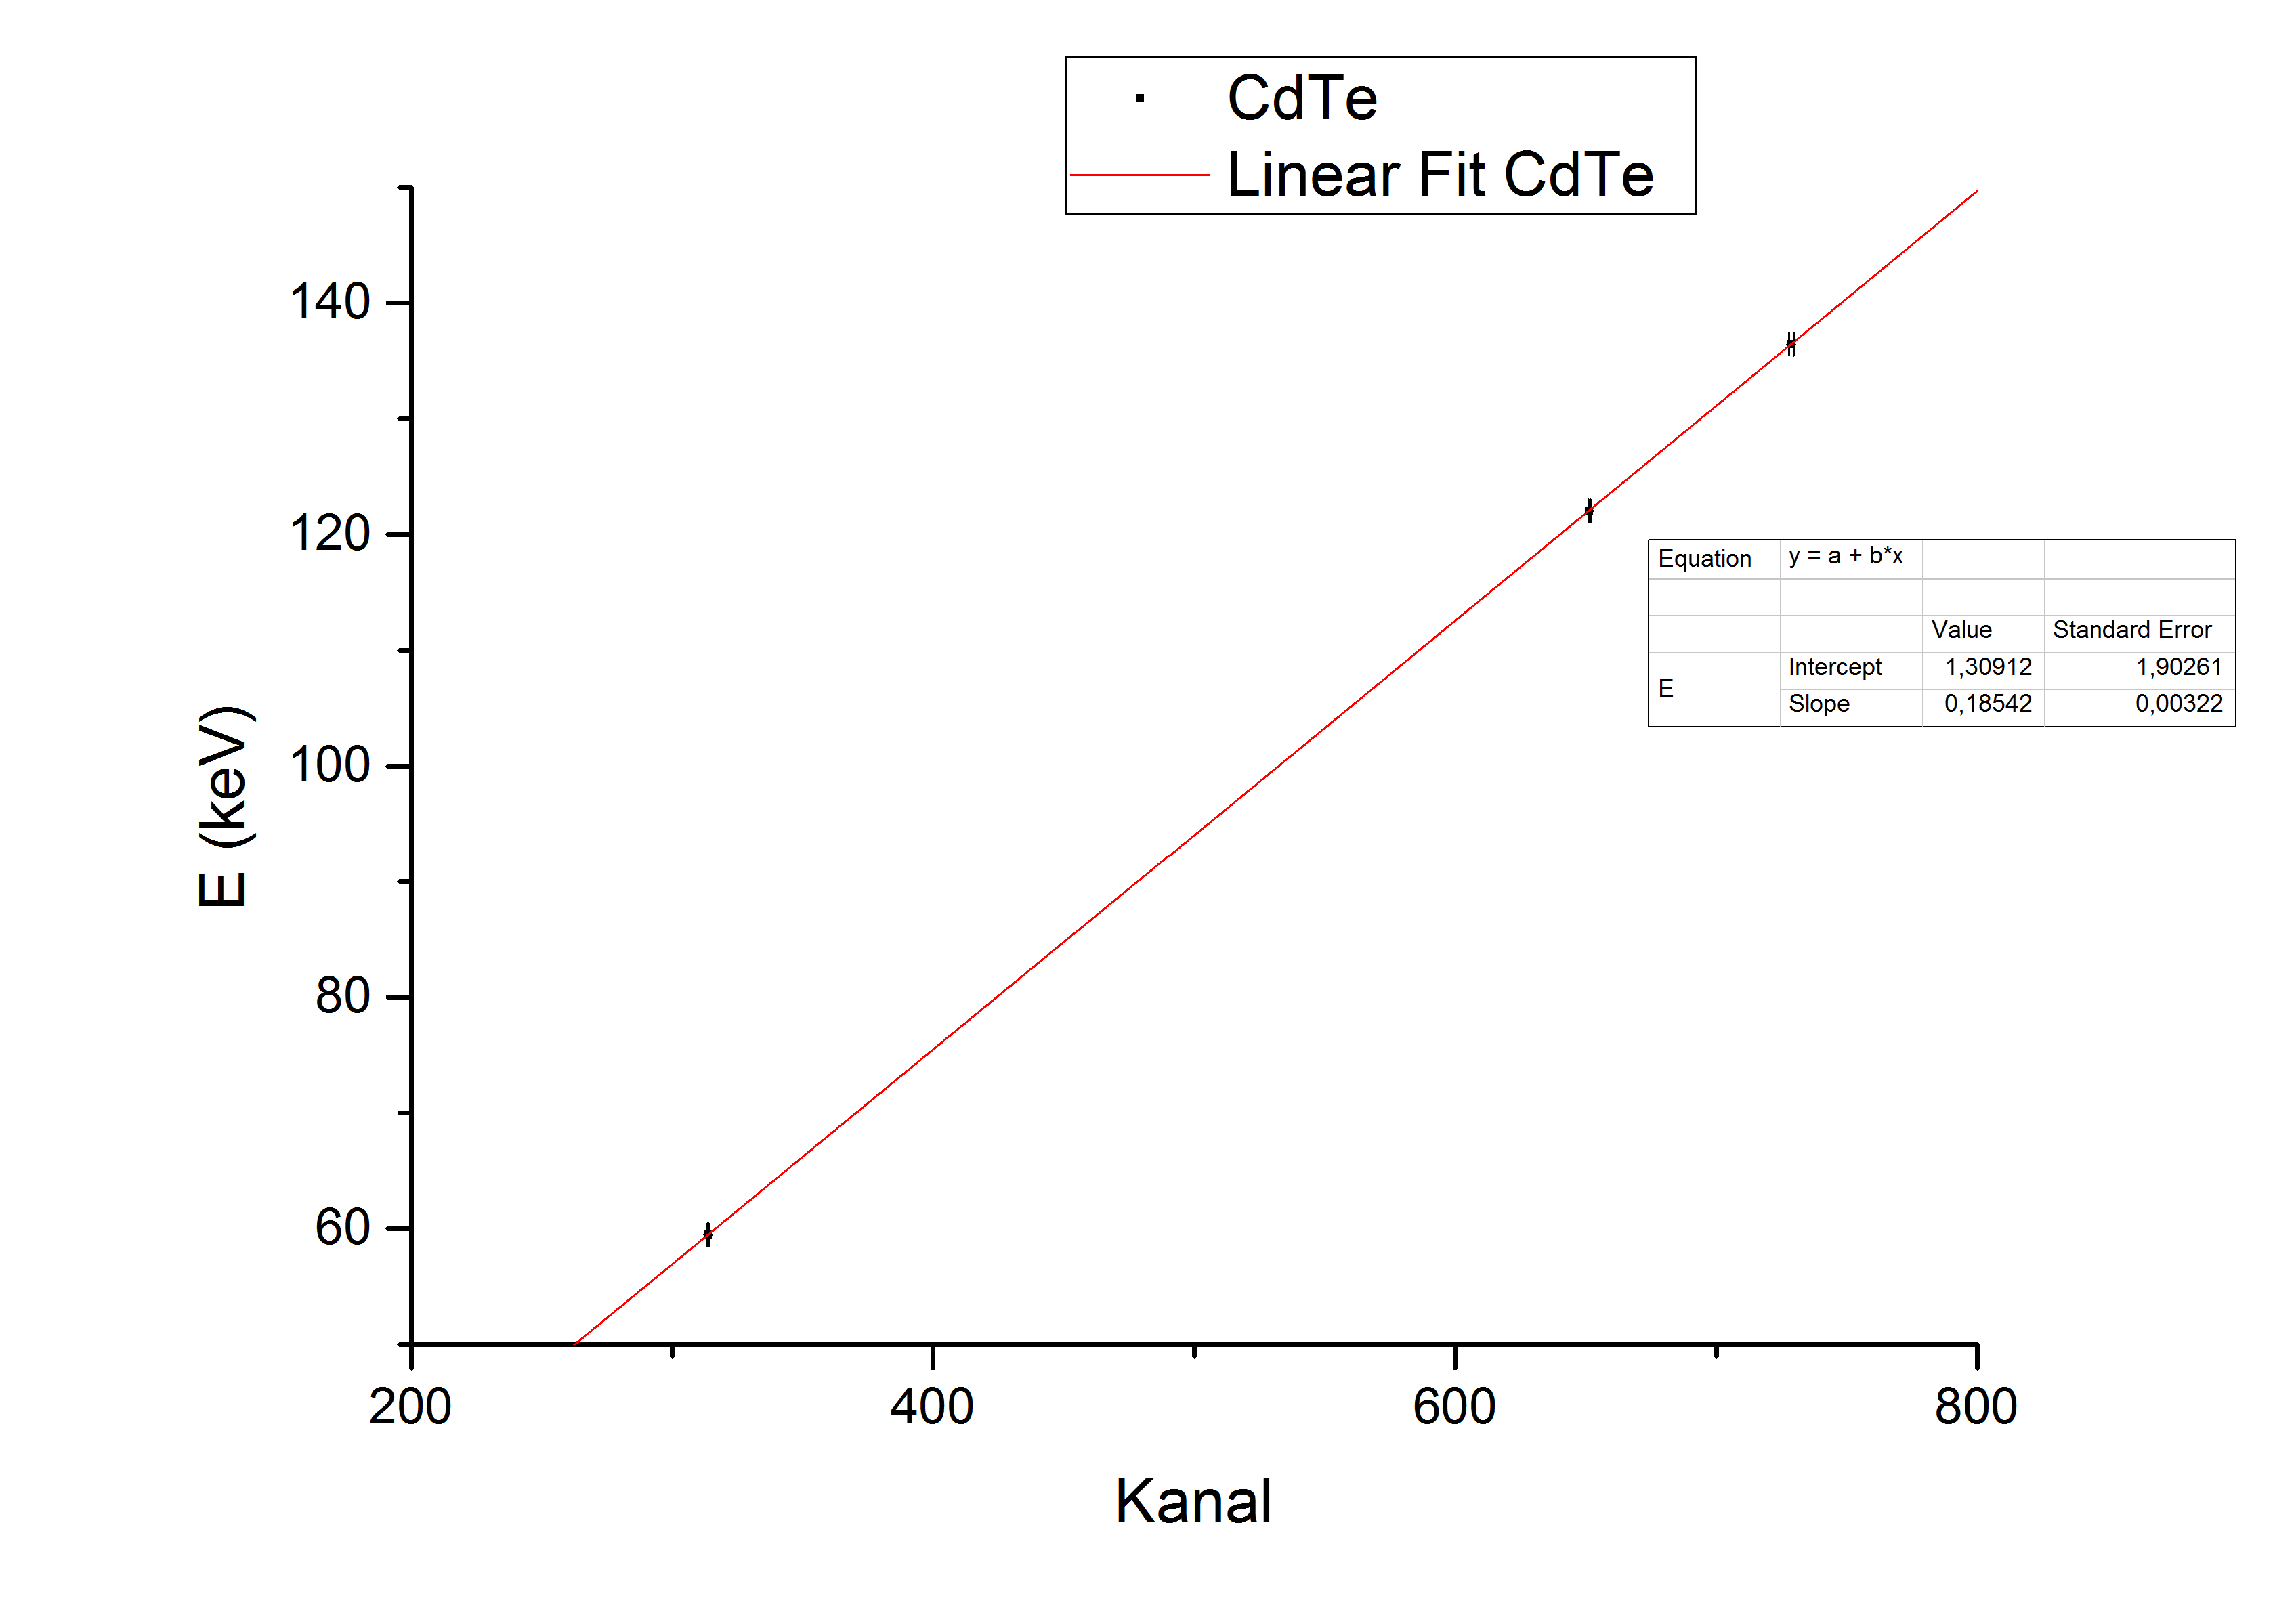
\includegraphics[scale=0.35]{Bilder/linfit_CdTe.png}\caption{Linear fit CdTe}\label{linfit_CdTe}
\end{center}
\end{figure}\\
\\
The energy calibration did obviously work well, as all the measured points can be connected very well with a linear fit.\\
\\
The goal of the experiment is now to compare the absorption probabilities and the energy resolutions of the Si- and CdTe-detector.\\
\\
\textbf{Absorption probability}\\
\\
To determine the ratio of the absorption probabilities of the detectors, we need a value A of the Gaussian fits, which is determined directly when doing the fit and tells us how many incidents occurred. It is $A=amplitude*\sqrt{2*\pi*\sigma^2}$. This value is divided by the surface area of the respective semiconductor detector, because this area is different for Si and CdTe $(a_{Si}=100mm^2, a_{CdTe}=23mm^2)$.\\
\\
It is:\\
\\
$\frac{A_{Si}/a_{Si}}{A_{CdTe}/a_{CdTe}}=\frac{Abs_{Si}}{Abs_{CdTe}}=R$\\
\\
$\Rightarrow$ The error is:\\
$s_{R}=\frac{Abs_{Si}}{Abs_{CdTe}}*\sqrt{(\frac{s_{A_{Si}}}{A_{Si}})^2+(\frac{s_{A_{CdTe}}}{A_{CdTe}})^2}$\\
\\
The results we got are in the table below:\\
\begin{table}[htbp]
  \centering
  \caption{Results}
    \begin{tabular}{rrrr}
    Energy in keV & Ratio R & Error s\_R & Literature value \\
    59,5  & 0,031 & 0,002 & 0,014 \\
    122,06 & 0,00023 & 0,00006 & 0,0183 \\
    136,47 & 0,000013 & 0,000009 & 0,02 \\
    \end{tabular}%
  \label{tab:addlabel}%
\end{table}%\\
\\
Obviously all our values, especially the ones for Co-57, are not even close to their respective literature values. This is not surprising regarding the fact that for silicon the spread for the peaks is just too large to do a proper Gaussian fit (see appendix). For 136,47 keV one needs some imagination to even see a peak at all: we'd rather say that what we measured there cannot really be called a peak. \\
There can be various causes for why our results aren't good: there's a systematic error as we neglect absorption in the epoxy layer. Also, because of the few counts for the 136,47 keV-peak (for Si) the noise is high, because of which the error of the Gaussian should be much larger than we actually determined it to be. Another cause could be an offset in the sample mounting: when changing the detectors, we had to remove the sample and put it back on, so that it's possible that there's a systematic error because we did not put back the sample to its former spot. It's also possible that there's some sort of problem with the sample or the electronics.\\
\\
\textbf{Energy resolution}\\
We can determine the energy resolution RER(E) of the detectors using the half-power width of the peaks. For our calculations we used the following formula:\\
\\
$RER(E)=\frac{FWHM(E)}{E} \approx 2,35\frac{\sigma_{E}}{E}$\\
\\
Because it is $E=a+b*channel$, we get the following:\\
\\$RER(E)=2,35\frac{\sqrt{s_{a}^2+channel^2*s_{b}^2+b^2*\sigma_{channel}^2}}{E}$\\
\\
$\Rightarrow s_{RER(E)}=RER(E)\frac{b^2*\sigma_{channel}*\sigma_{\sigma_{channel}}}{\sigma(E)}}$\\
This way we get the following for the energy resolution:\\
\\
\\
\\
\\
\\
\\
\\
\\
\\
\caption{Energy resolutions}
    \begin{tabular}{rrrr}
    Detector & Energy in keV & RER[E]  & s\_RER[E] \\
    Si    & 59,5  & 0,121 & 0,003 \\
          & 122,06 & 0,068 & 0,007 \\
          & 136,47 & 0,05229 & 0,00005 \\
    CdTe  & 59,5  & 0,118  & 0,006 \\
          & 122,06 & 0,060 & 0,005 \\
          & 136,47 & 0,07  & 0,04 \\
    \end{tabular}%
  \label{tab:addlabel}%
\\
Although we don't have literature values given here, obviously because of the errors listed above these won't be good results. Still, at least for Si we could prove a general tendency: the larger the energy is, the better is the resolution. Obviously the error for the third value of the Si-detector is way too low, which is due to the fact that there is not really a peak, making the Gaussian fit having a too small width.






\chapter{Summary}
\section{Measuring the Bandgap}
In experiment no. 1 we determined the bandgap energy of Si and Ge respectively. Our results are:\\
\begin{center}
$E_{Si}=(1,087\pm 0,018)$eV ; literature value: 1,12 eV (source: [Ver])\\
$E_{Ge}=(0,64\pm0,03)$eV; literature value: 0,67 eV (source: [Ver])\\
\end{center}
Both these values are, especially regarding the fact that the errors are certainly too small (see analysis for further information) good. \\
\section{Haynes-Shockley-experiment}
This experiment consisted of two different approaches: in the first part we modified the distance, in the second the voltage applied.\\
The results were the following:\\
First part:\\
\begin{center}
Mobility $\mu=(2420\pm 70)\frac{cm^2}{Vs}$\\
Mean lifetime $\tau=(2,4\pm 0,1)*10^-6 s$\\
Diffusion constant $D_{n}=(5\pm1)*10^-8 \frac{mm^2}{s}$
\end{center}
Second part:\\
\begin{center}
Mobility $\mu=(2600\pm 400) \frac{cm^2}{Vs}$\\
Mean lifetime $\tau=(2,0\pm 0,6)*10^-6 s$\\
Diffusion constant $D_{n}=(0,3\pm9,1)*10^-8 \frac{mm^2}{s}$
\end{center}
~\\
The literature values are the following:\\
\begin{center}
Mobility $\mu=3900 \frac{cm^2}{Vs}$\\
Mean lifetime $\tau=(45\pm 2)*10^-6 s$\\
Diffusion constant $D_{n}=101 \frac{cm^2}{s}$
\end{center}
~\\
The values for $\mu$ are in the same order of magnitude as the literature values. This does not hold for $\tau$ and especially not for the diffusion constant $D_{n}$. Further explanations and possible reasons can be found in the analysis of this part of the experiment.\\
~\\
\section{Semiconductor detectors}
In this section, our task was to measure the spectra of two radioactive sources (Am-241 and Co-57) with the semiconductor detectors Si and CdTe respectively.\\
The results for the ratio of the absorption probabilities of Si and CdTe for different energies were the following:\\
\begin{table}[htbp]
  \centering
  \caption{Results}
    \begin{tabular}{rrrr}
    Energy in keV & Ratio R & Error s\_R & Literature value \\
    59,5  & 0,031 & 0,002 & 0,014 \\
    122,06 & 0,00023 & 0,00006 & 0,0183 \\
    136,47 & 0,000013 & 0,000009 & 0,02 \\
    \end{tabular}%
  \label{tab:addlabel}%
\end{table}%\\
~\\
As already discussed, we might have had some kind of trouble with the setup. \\
~\\
Our second task was to calculate the energy resolutions of the semiconductor detectors:\\
~\\
  \caption{Energy resolutions}
      \begin{tabular}{rrrr}
      Detector & Energy in keV & RER[E]  & s\_RER[E] \\
      Si    & 59,5  & 0,121 & 0,003 \\
            & 122,06 & 0,068 & 0,007 \\
            & 136,47 & 0,05229 & 0,00005 \\
      CdTe  & 59,5  & 0,118  & 0,006 \\
            & 122,06 & 0,060 & 0,005 \\
            & 136,47 & 0,07  & 0,04 \\
      \end{tabular}%
    \label{tab:addlabela}%
~\\
  The expected general tendency could at least for Si be shown. For CdTe it's obvious that the value for 59,5 keV is - as expected - higher as those for the peaks of Co-57. Unfortunately it's difficult to distinguish between the peaks of Co-57.

\newpage
\chapter{Bibliography}
~\\
[Amr] Simon Amrein, Staatsexamensarbeit: "Halbleiter und Halbleiterdetektoren", 2008\\
[Ver] Versuchsanleitung, Fortgeschrittenen-Praktikum für Physiker,Uni-Freiburg\\
[Sclo] http://www.scilogs.de/wblogs/gallery/59/previews-med/720px-Isolator-metal.png\\
\chapter{Appendix}
\section*{Experiment No.1}
\subsection*{Germanium}
\begin{figure}[h]
\begin{center}
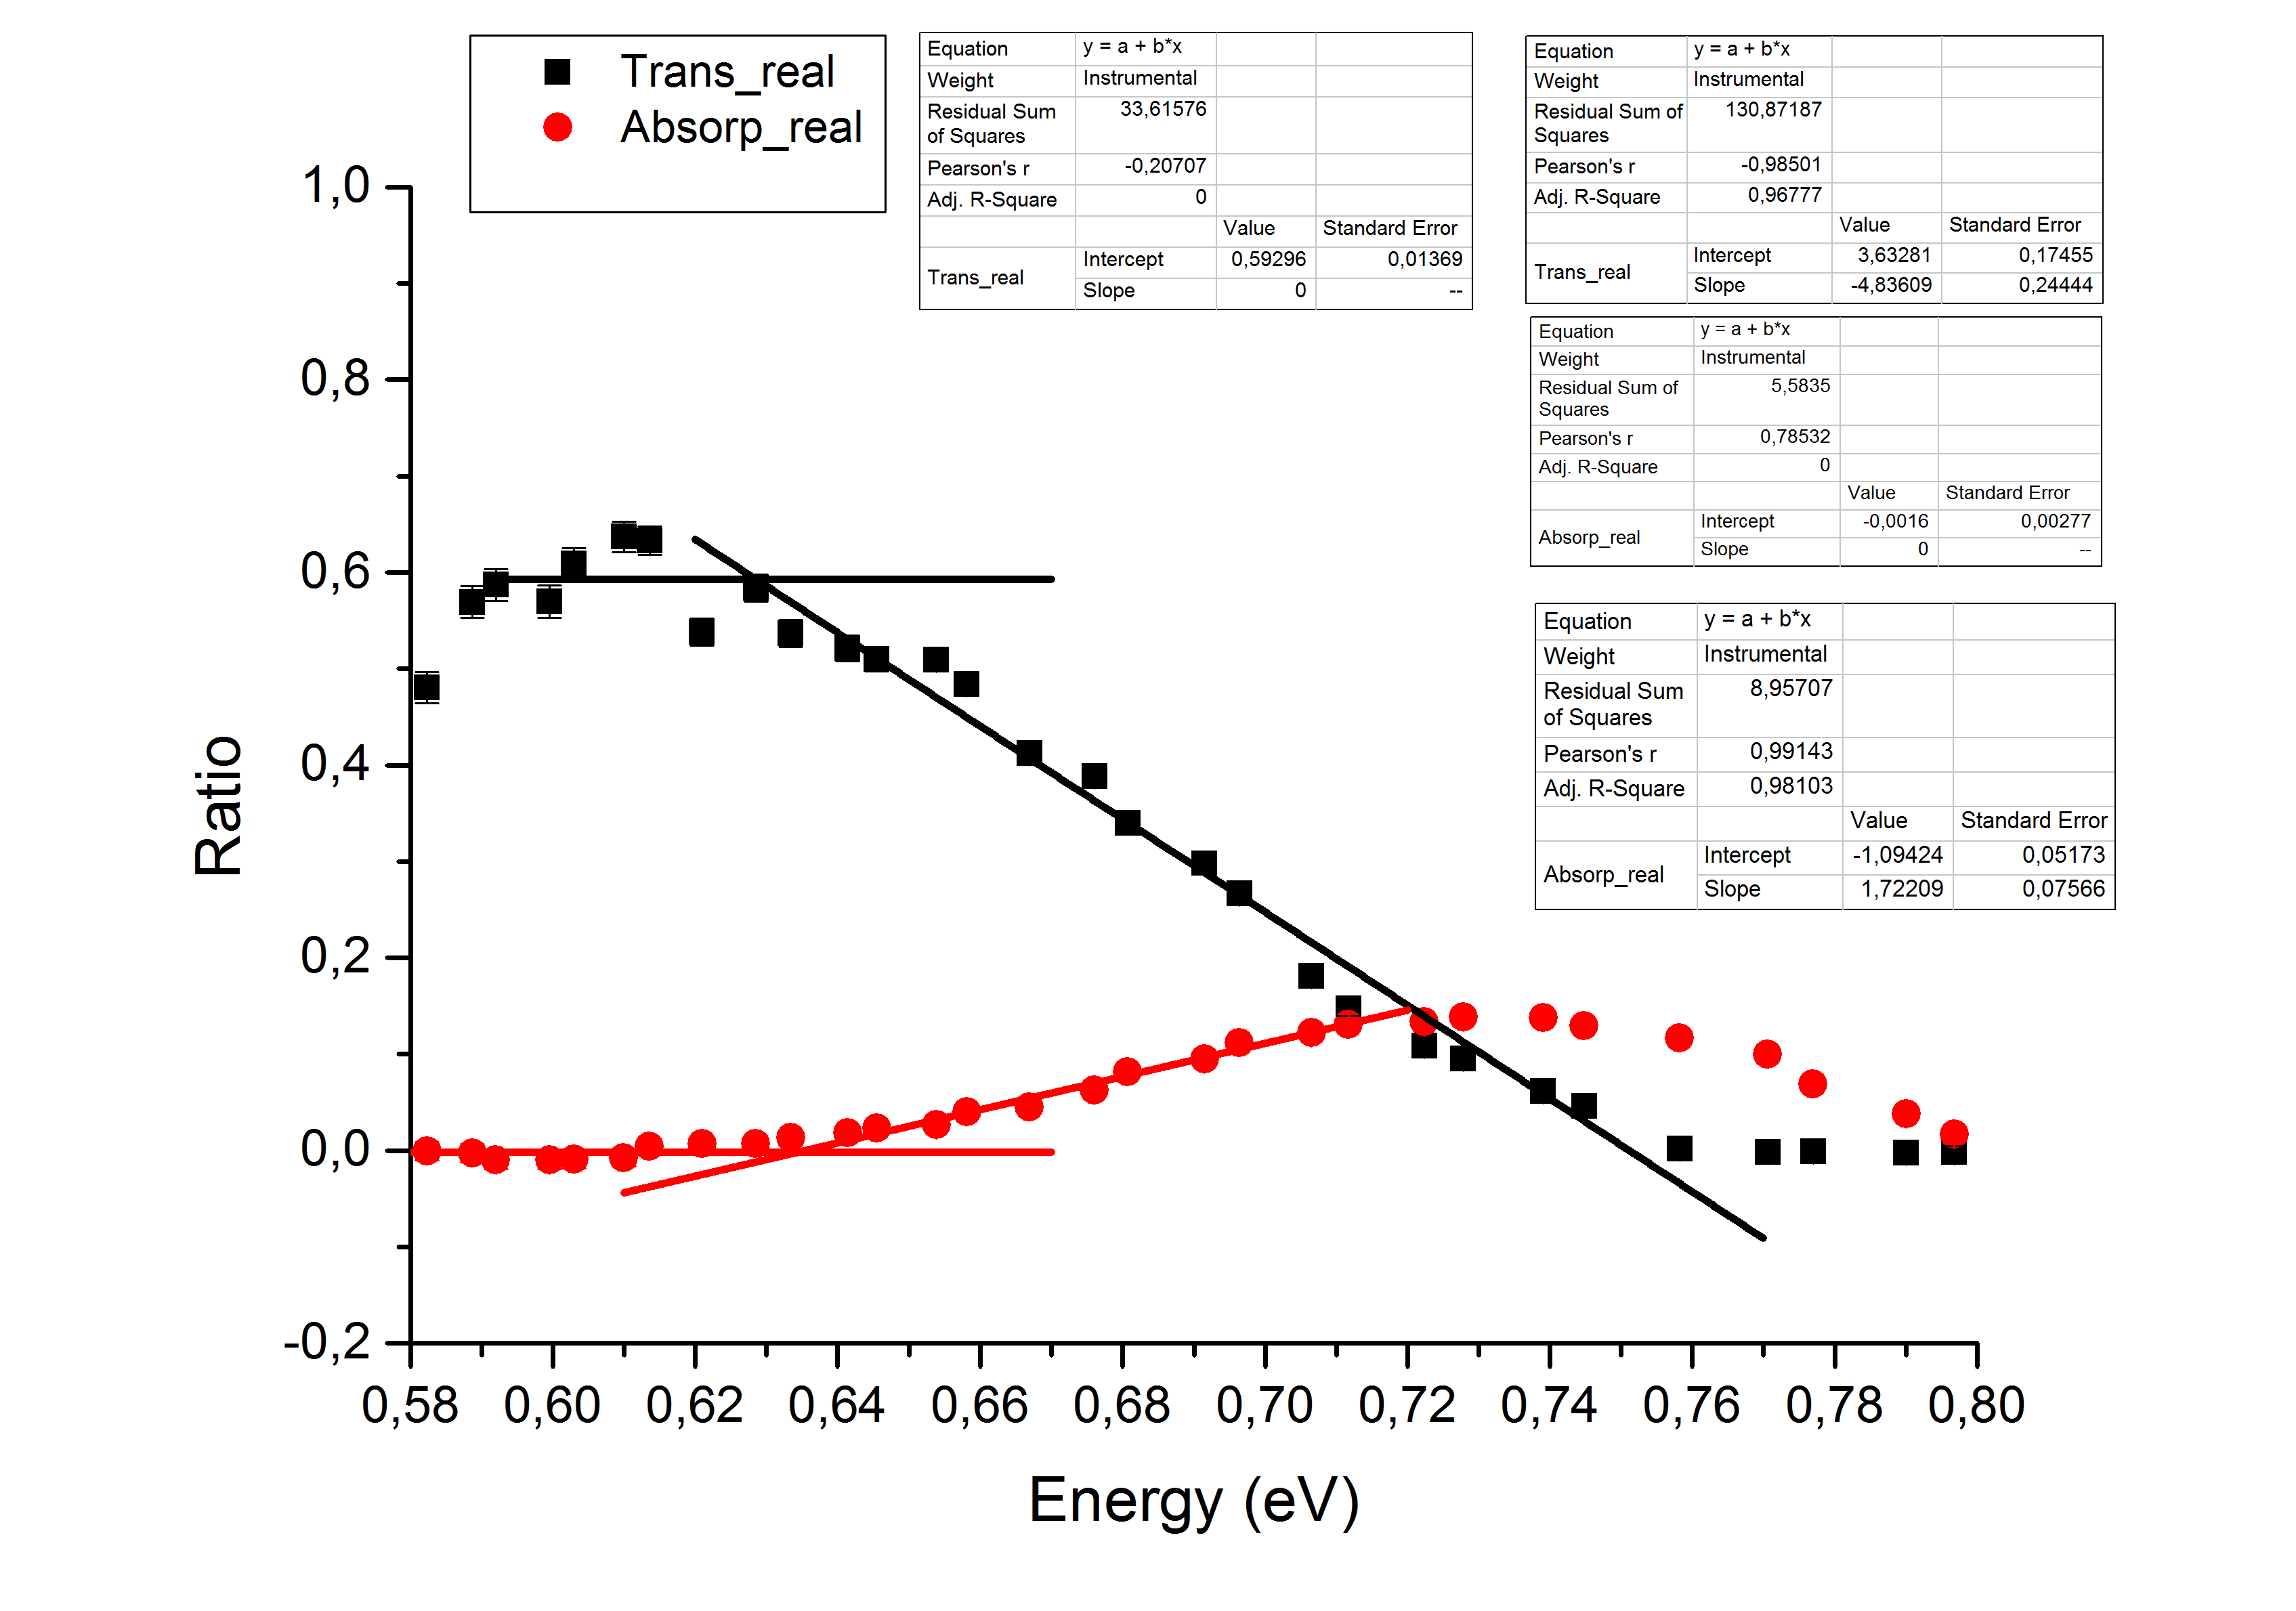
\includegraphics[scale=0.25]{Bilder/Teil1/V1_Ge_positiv}
\caption{Positive fit section of Germanium}
\label{fig:GePo}
\end{center}
\end{figure}
\begin{figure}[h]
\begin{center}
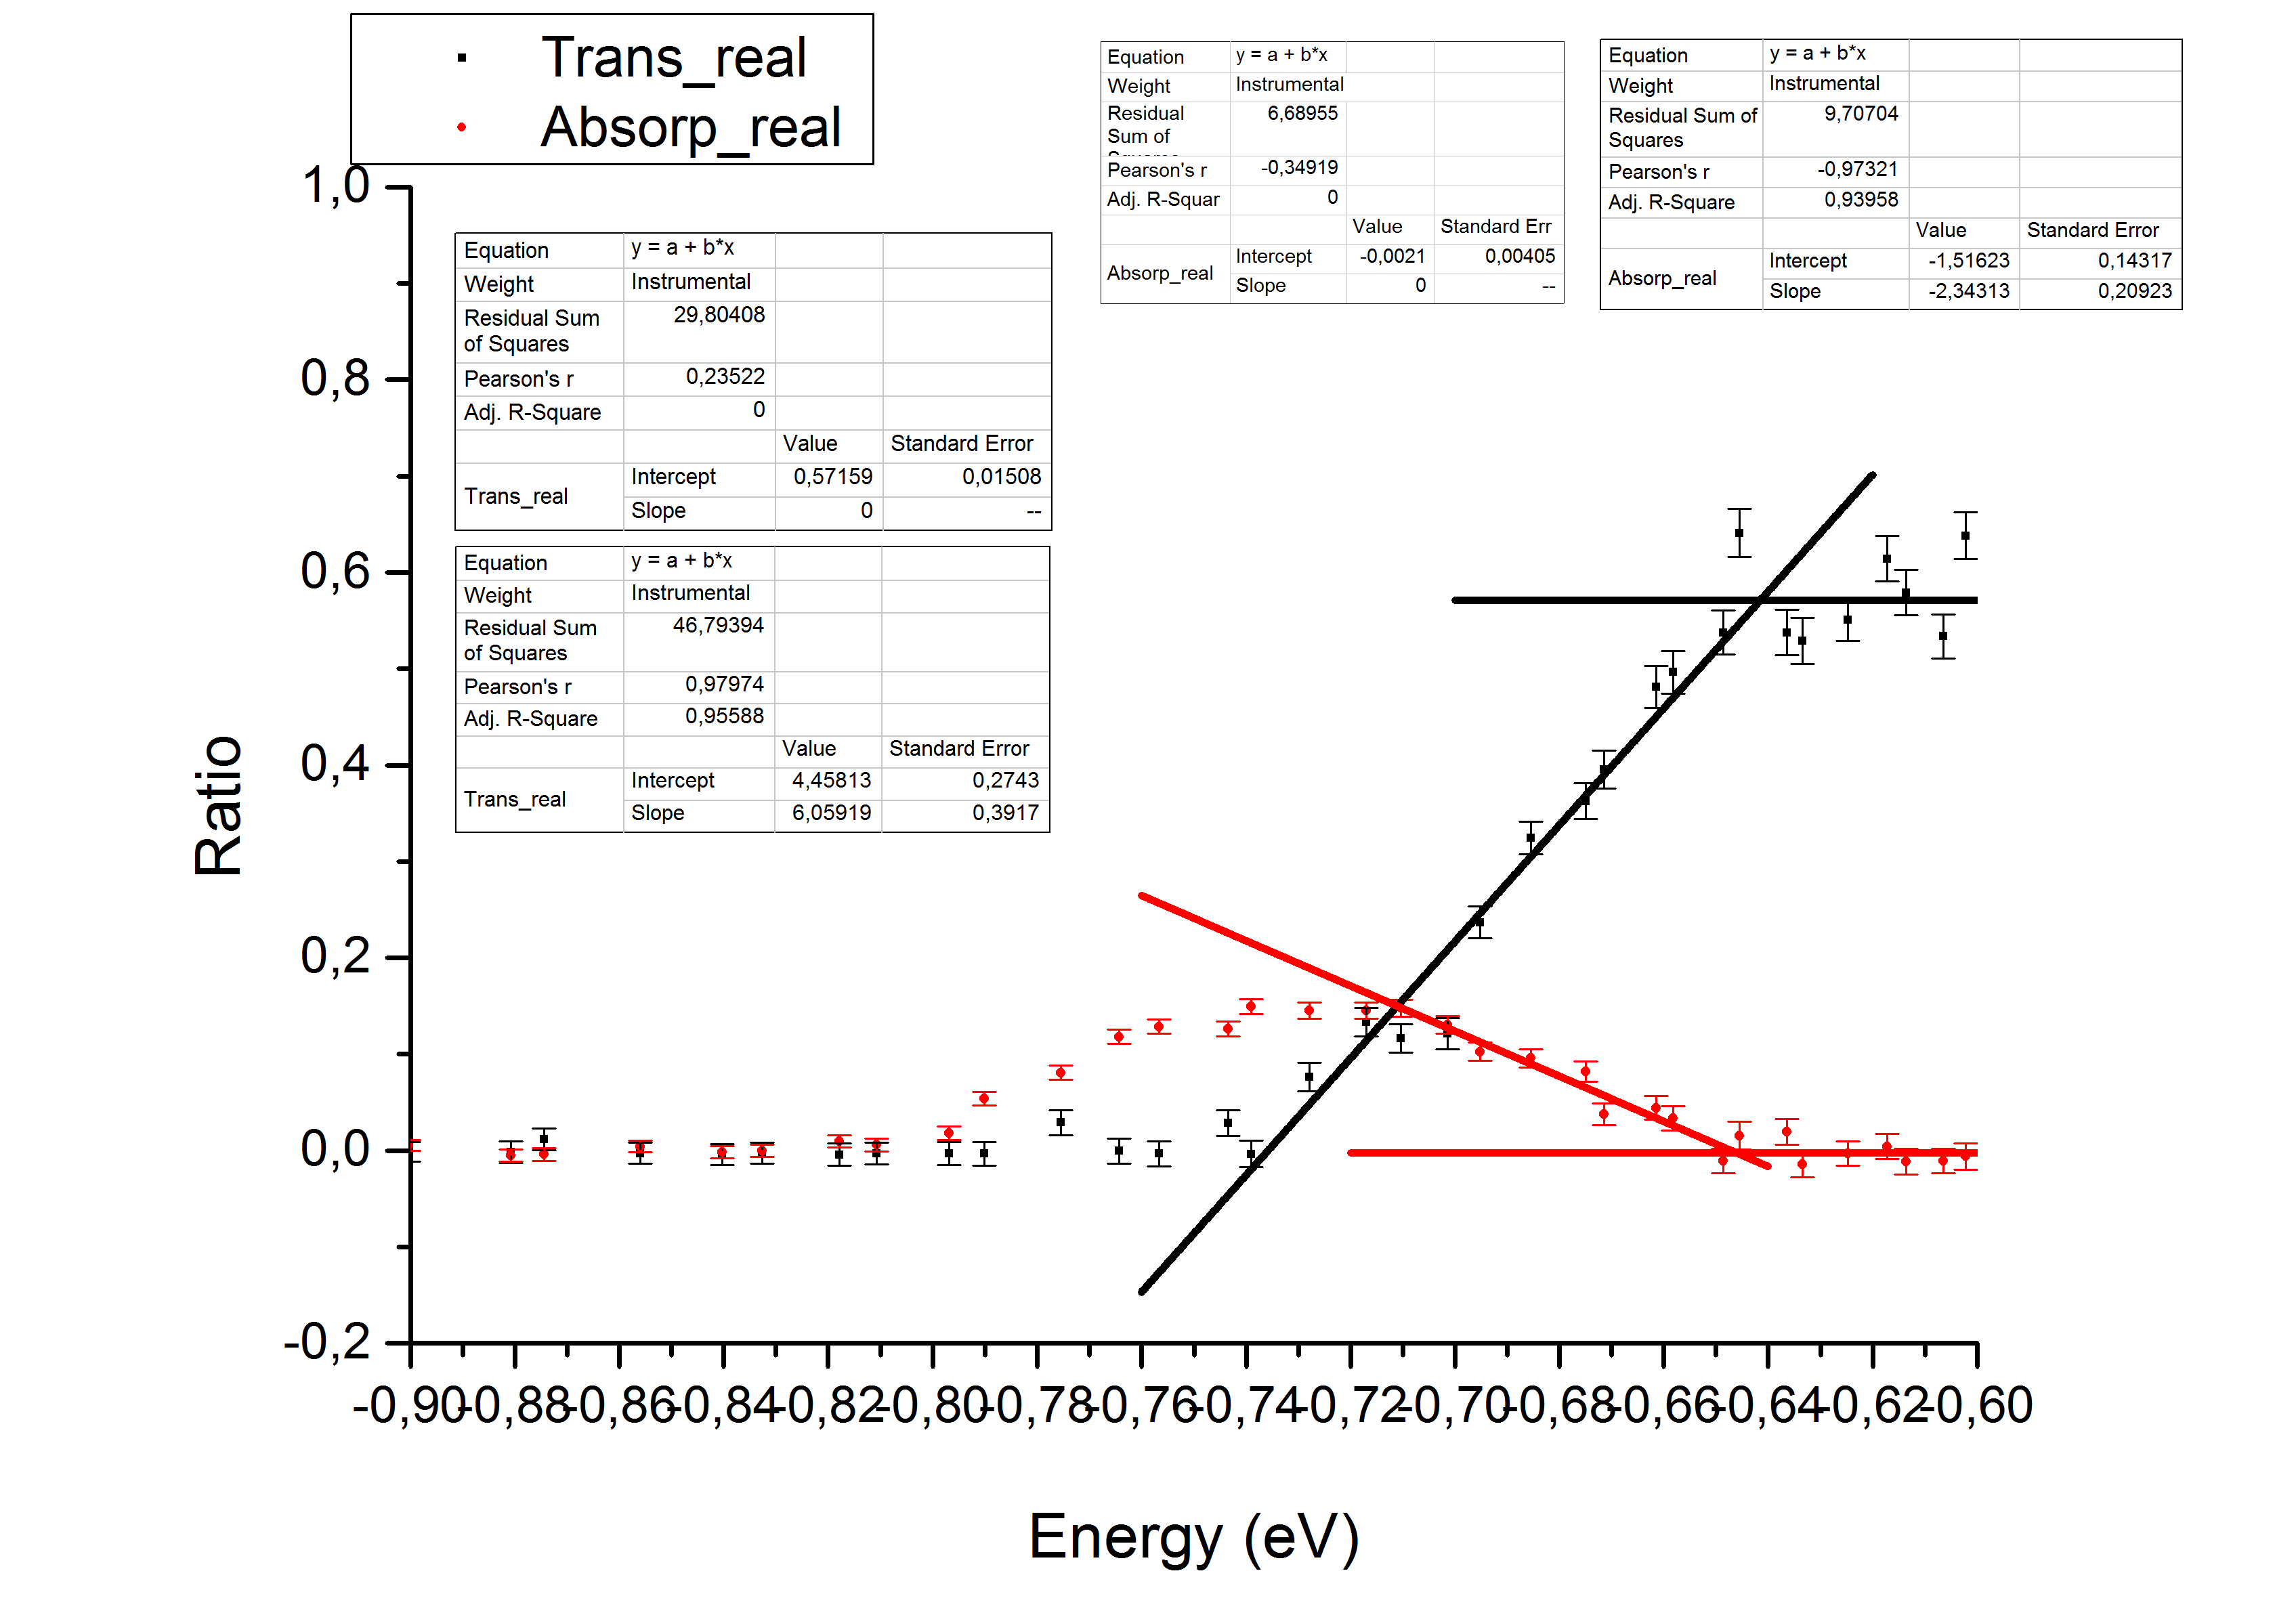
\includegraphics[scale=0.25]{Bilder/Teil1/V1_Ge_negativ}
\caption{Negative fit section of Germanium}
\label{fig:GePo}
\end{center}
\end{figure}
\subsection*{Silicon}
\begin{figure}[h]
\begin{center}
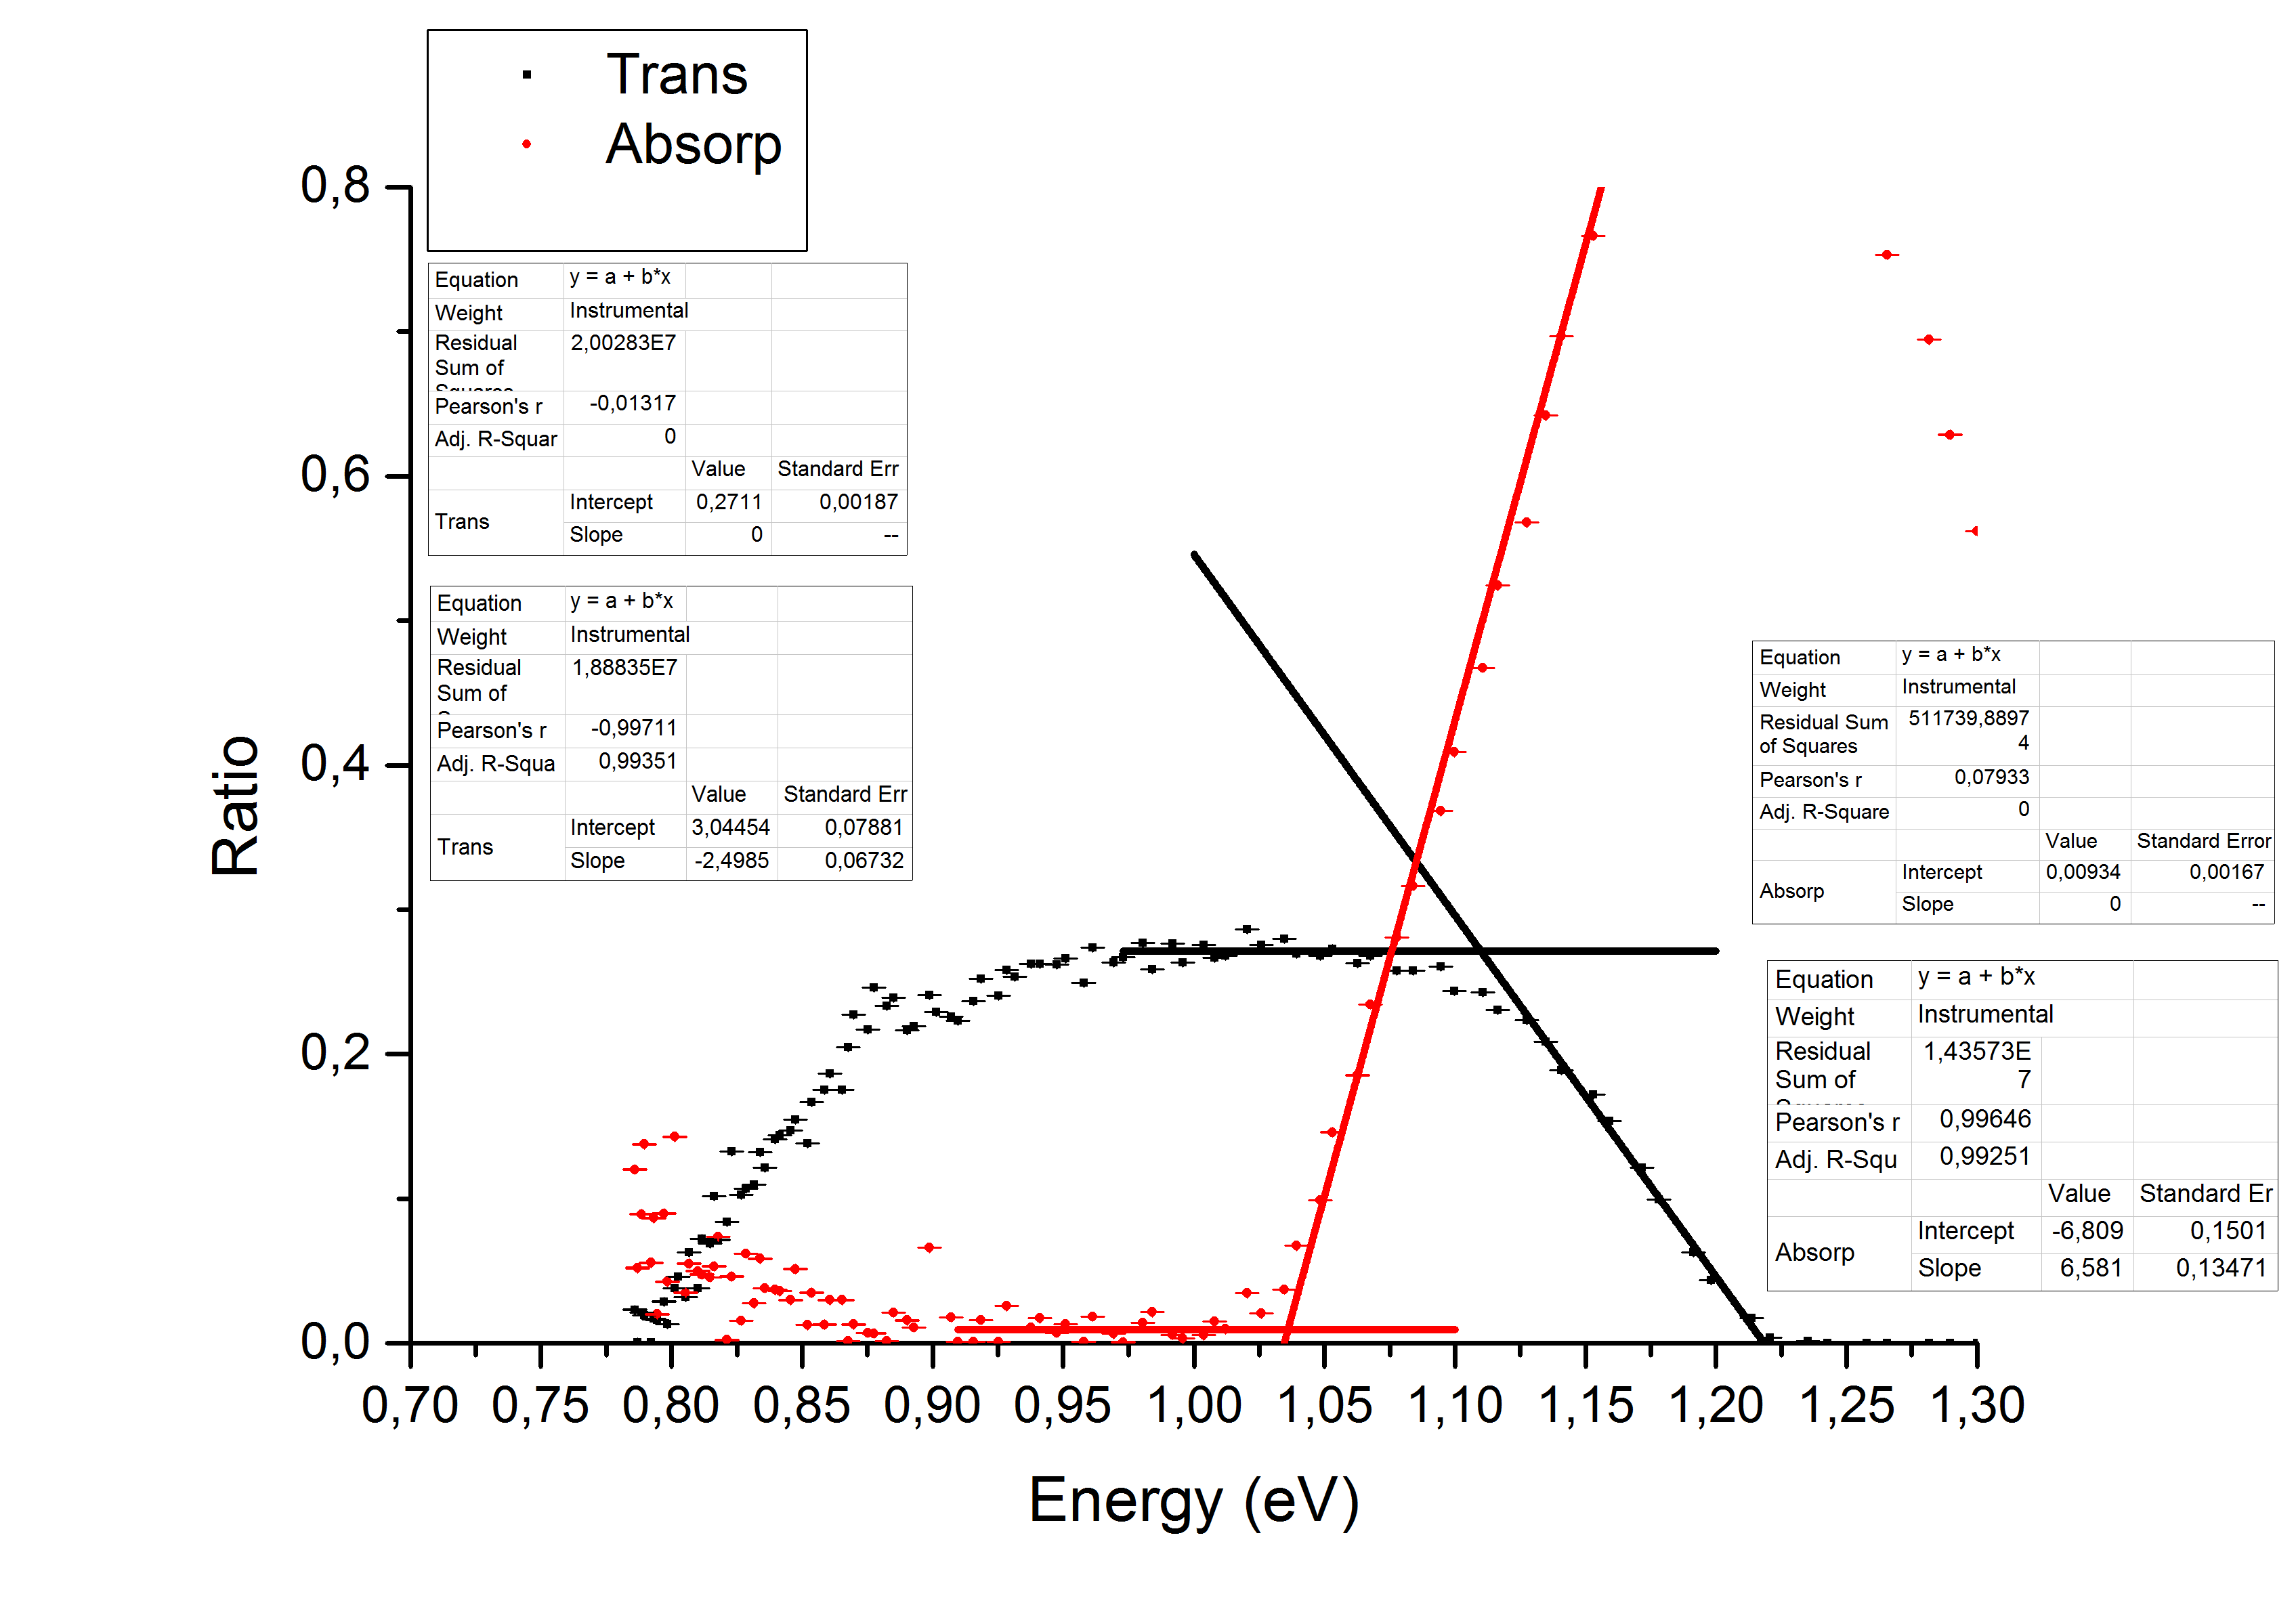
\includegraphics[scale=0.25]{Bilder/Teil1/V1_Si_positiv}
\caption{Positive fit section of Silicon}
\label{fig:SiPo}
\end{center}
\end{figure}
\begin{figure}[ht!]
\begin{center}
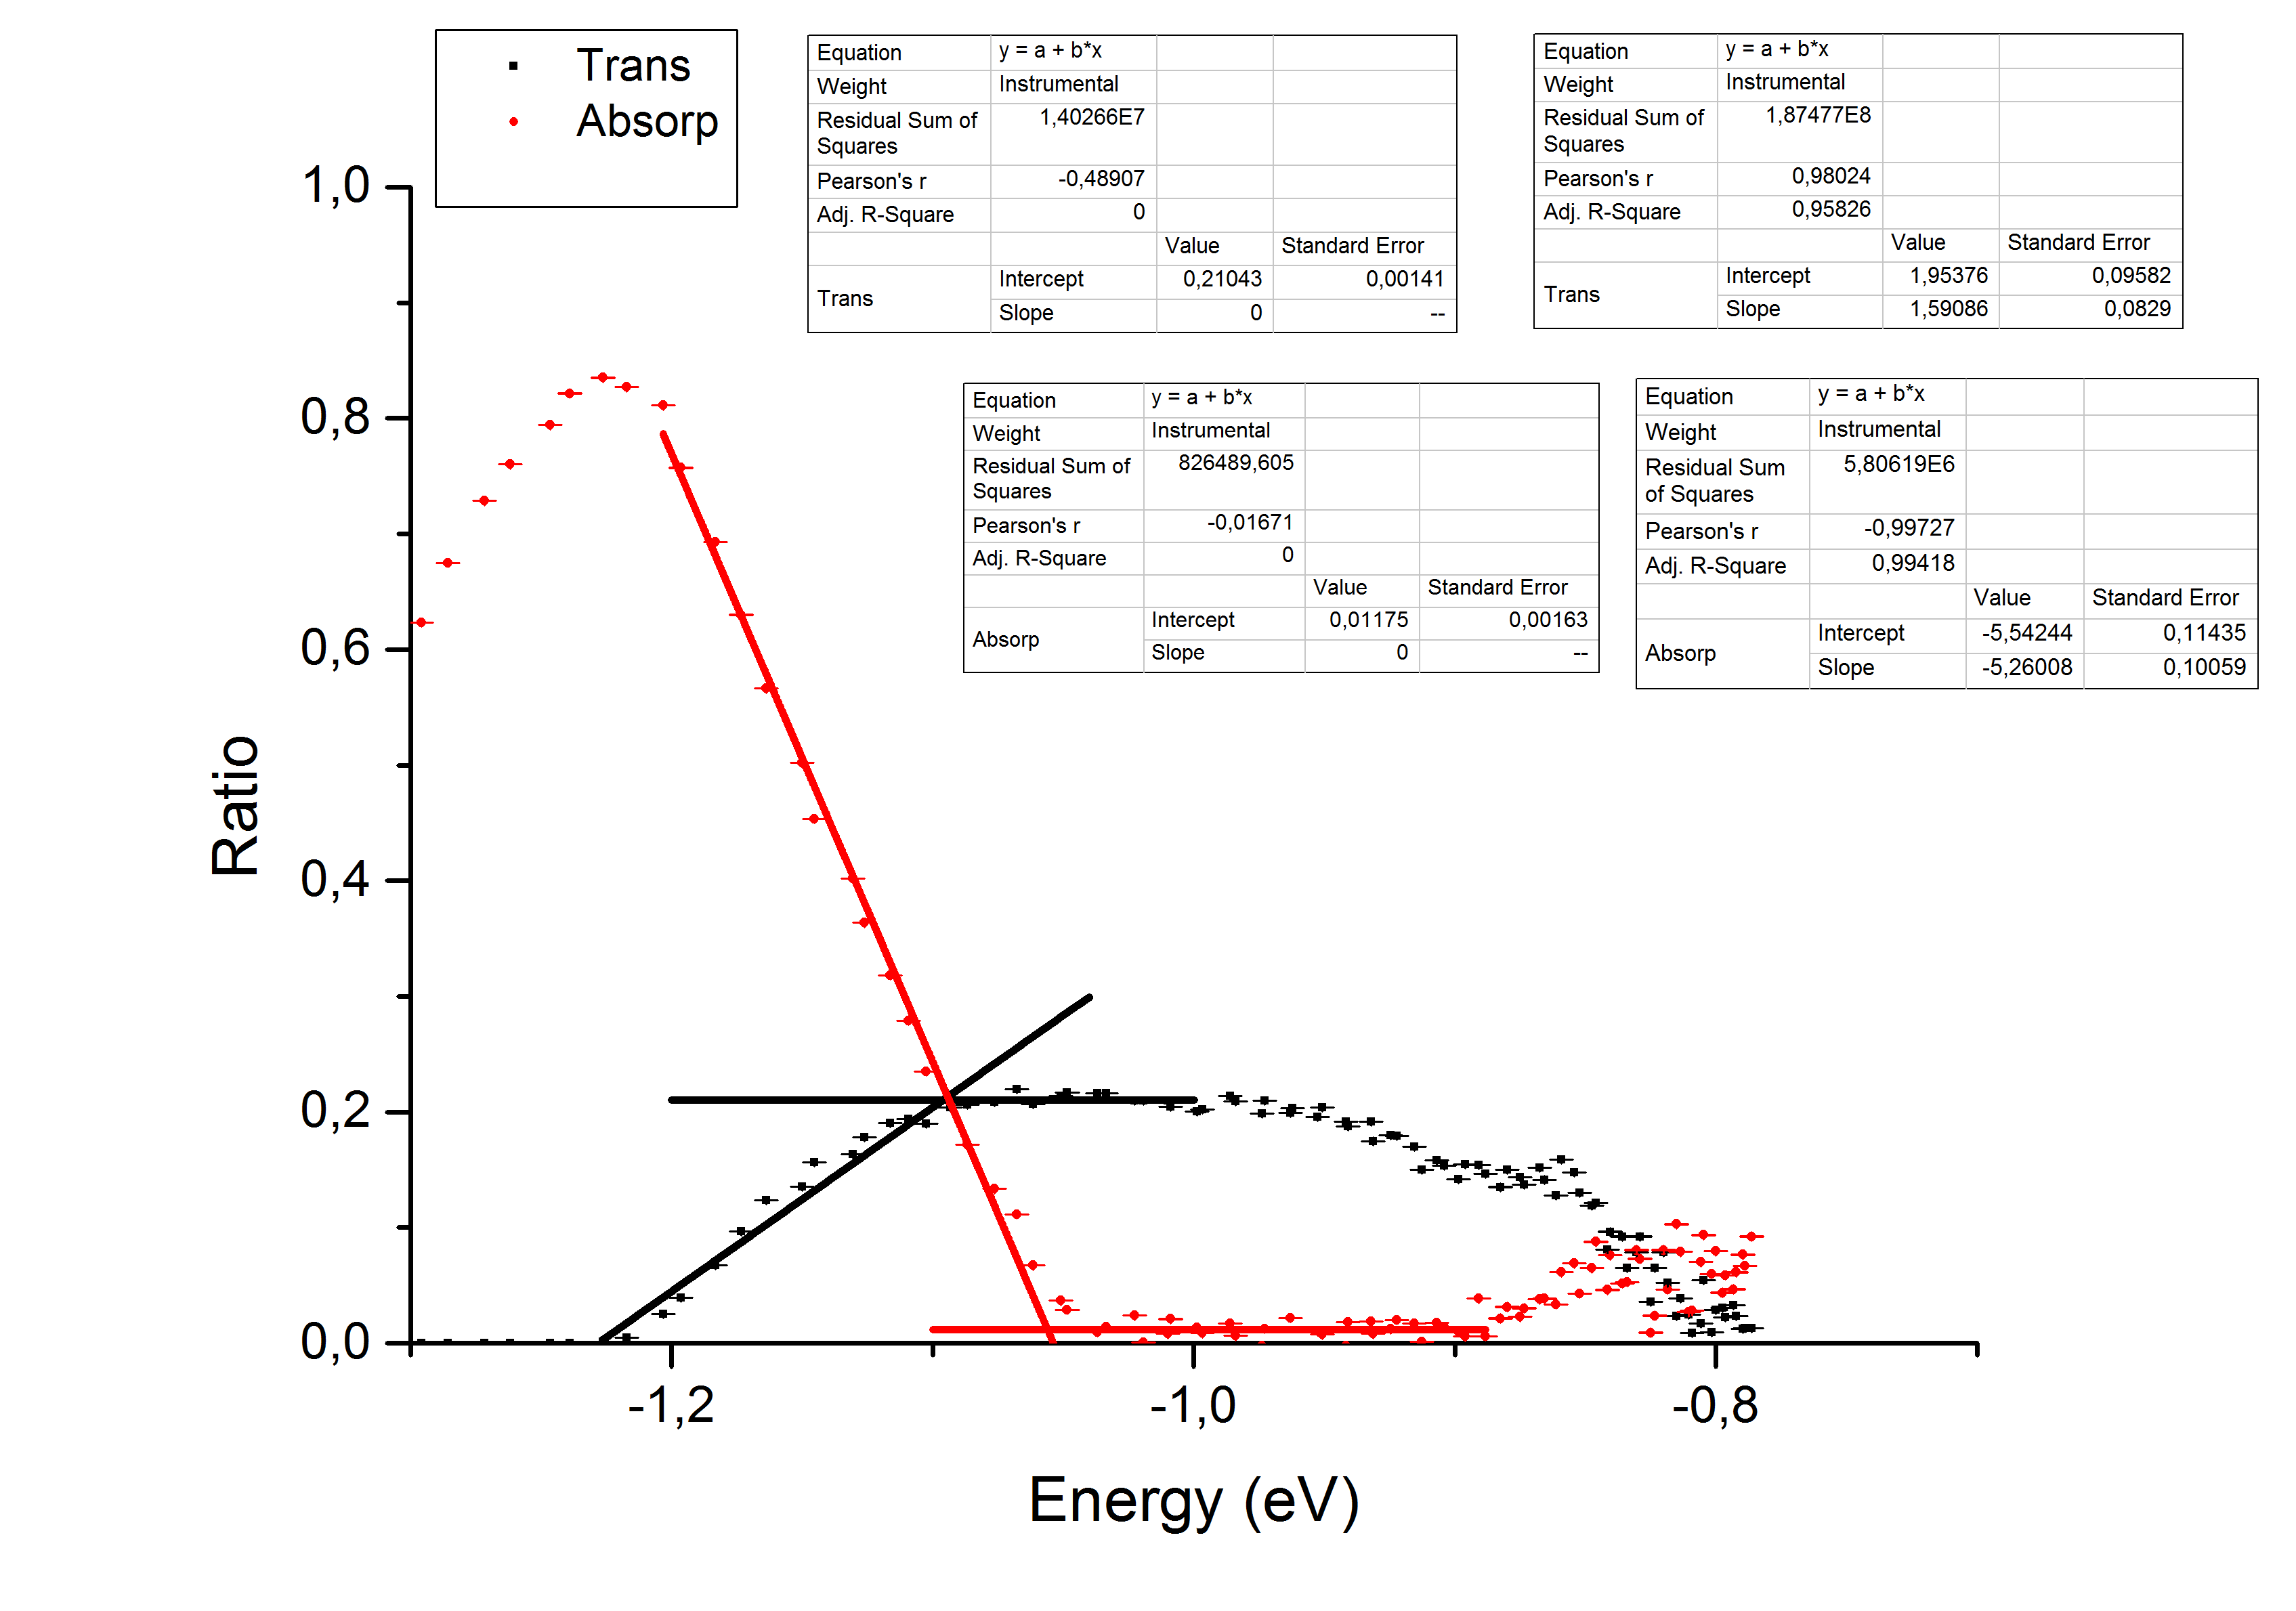
\includegraphics[scale=0.25]{Bilder/Teil1/V1_Si_negativ}
\caption{Negative fit section of Silicon}
\label{fig:SiNe}
\end{center}
\end{figure}
\section*{Experiment No.2}
\subsection*{First series of measurements}
\begin{figure}[h]
\begin{center}
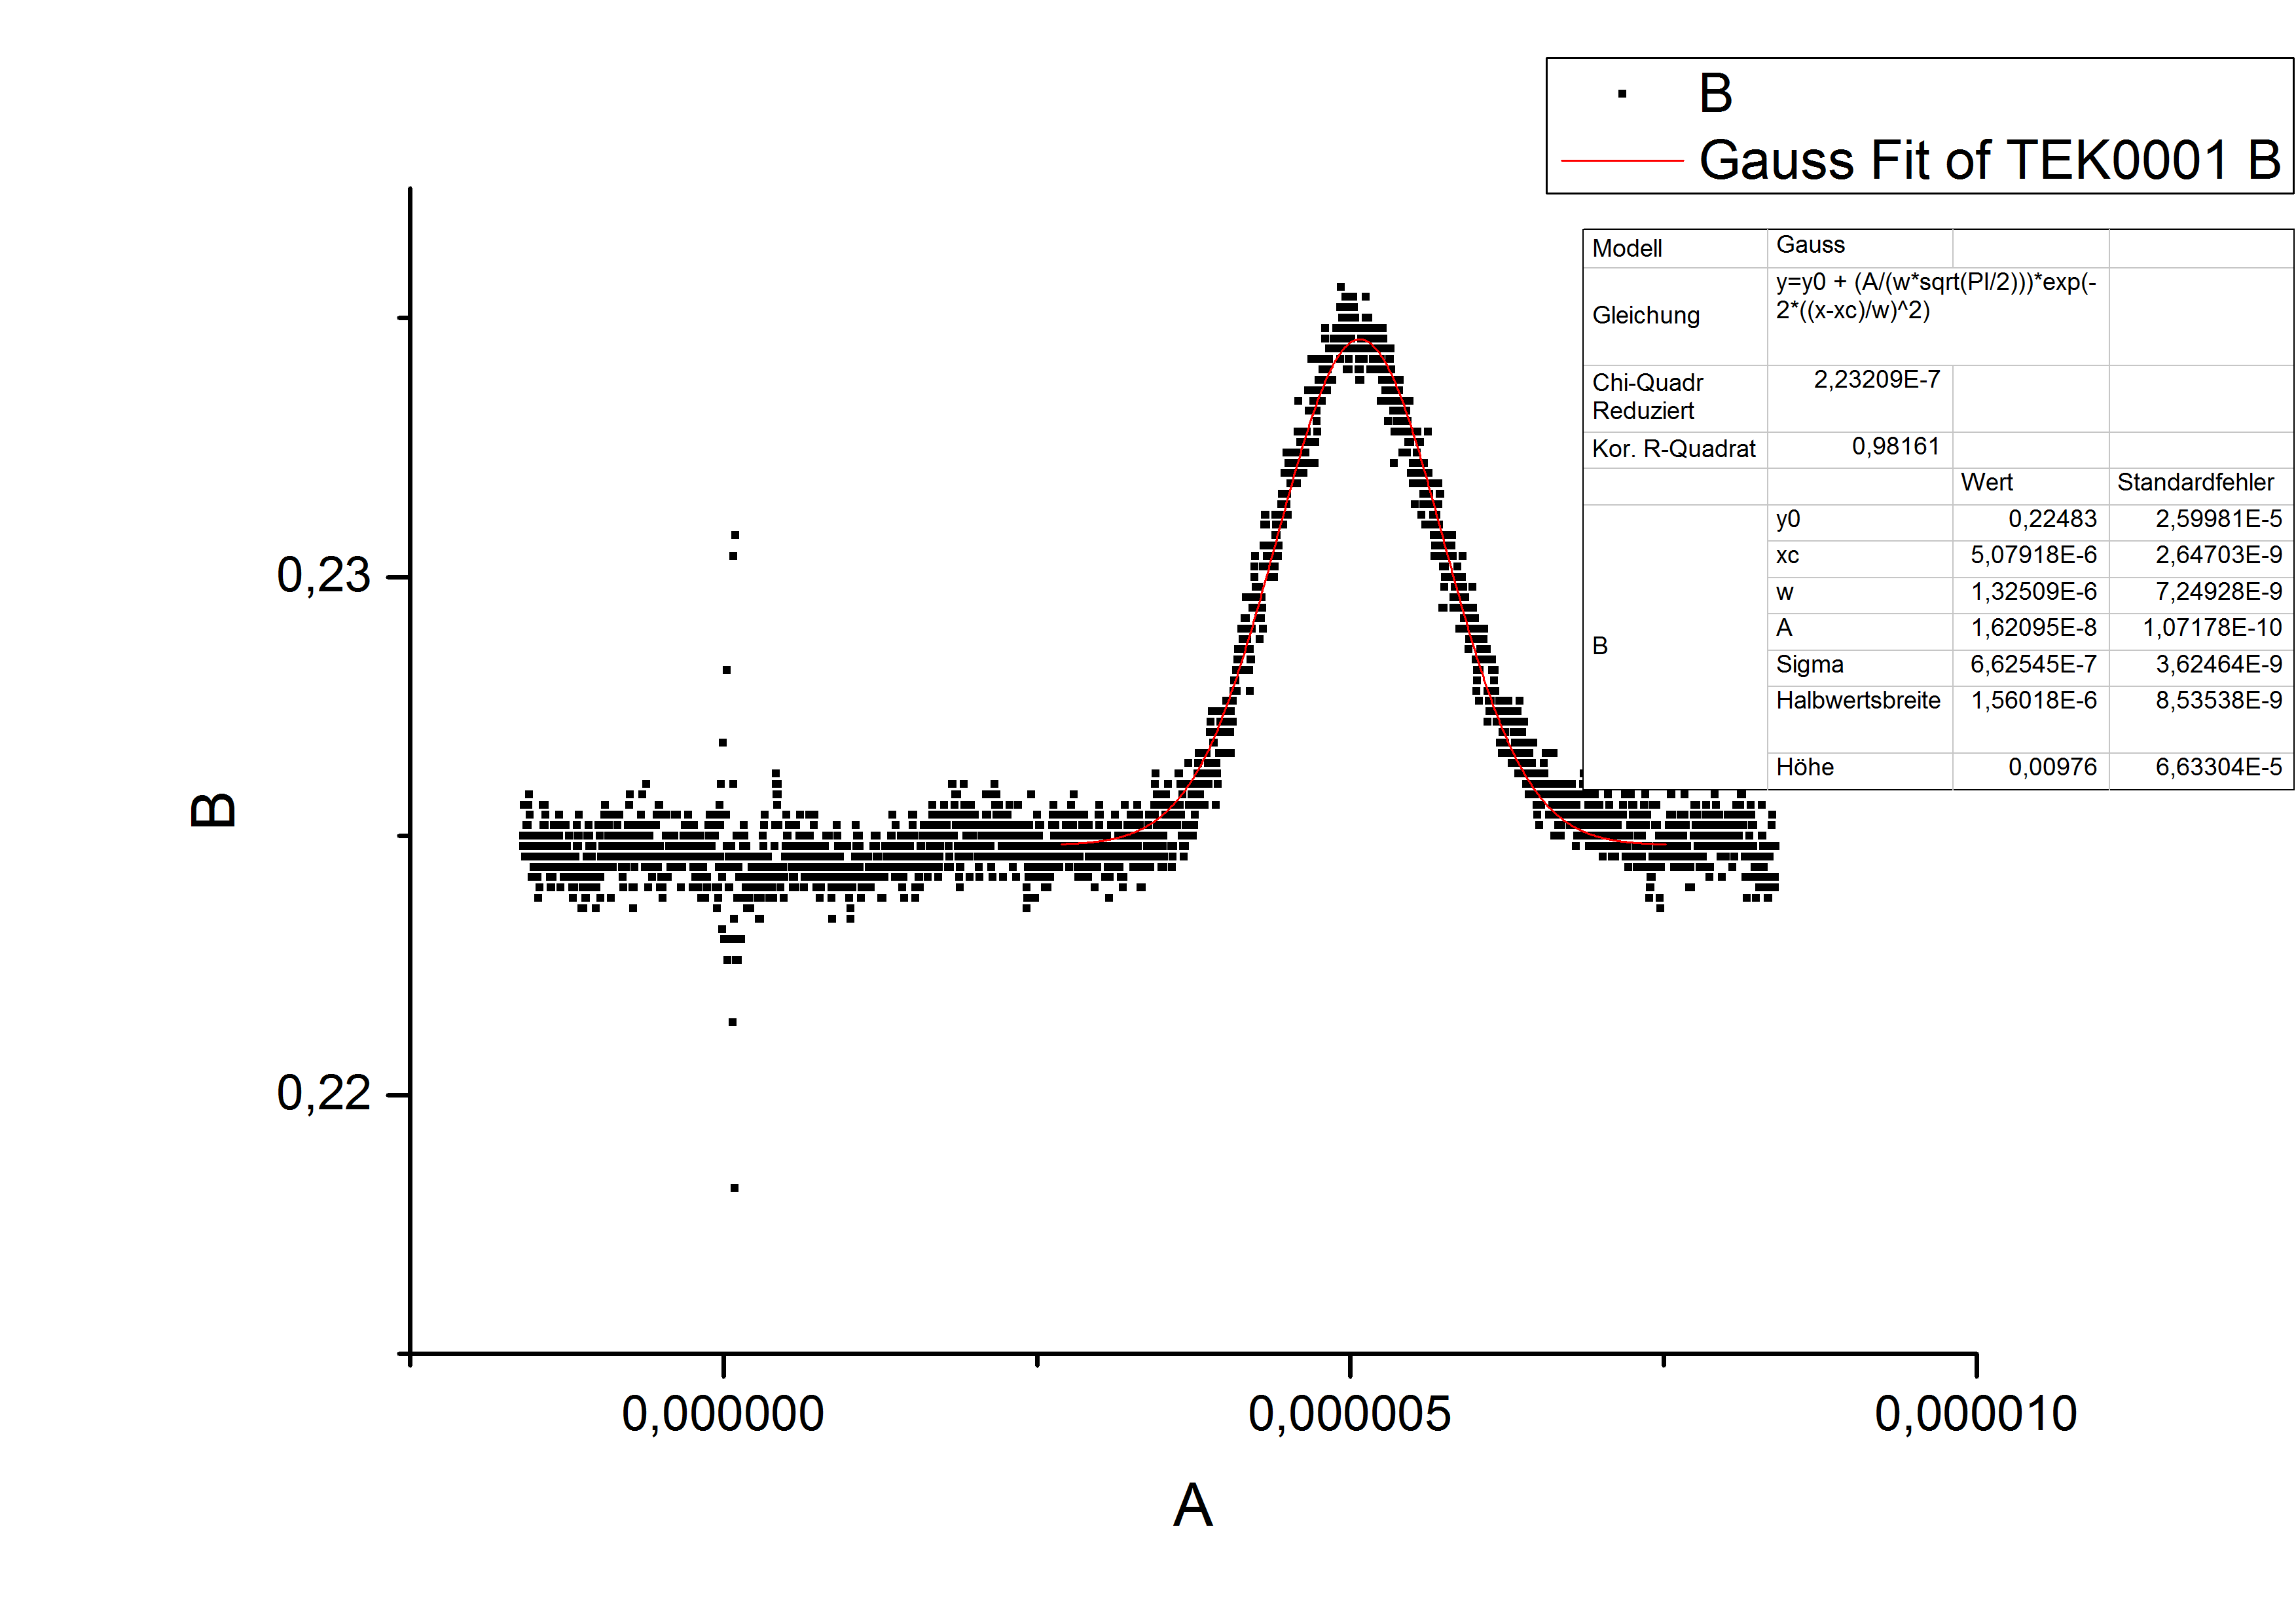
\includegraphics[scale=0.25]{Bilder/Teil2/Graph1}
\caption{Graph at 2.52mm.}
\label{fig:graph1}
\end{center}
\end{figure}
\begin{figure}[h]
\begin{center}
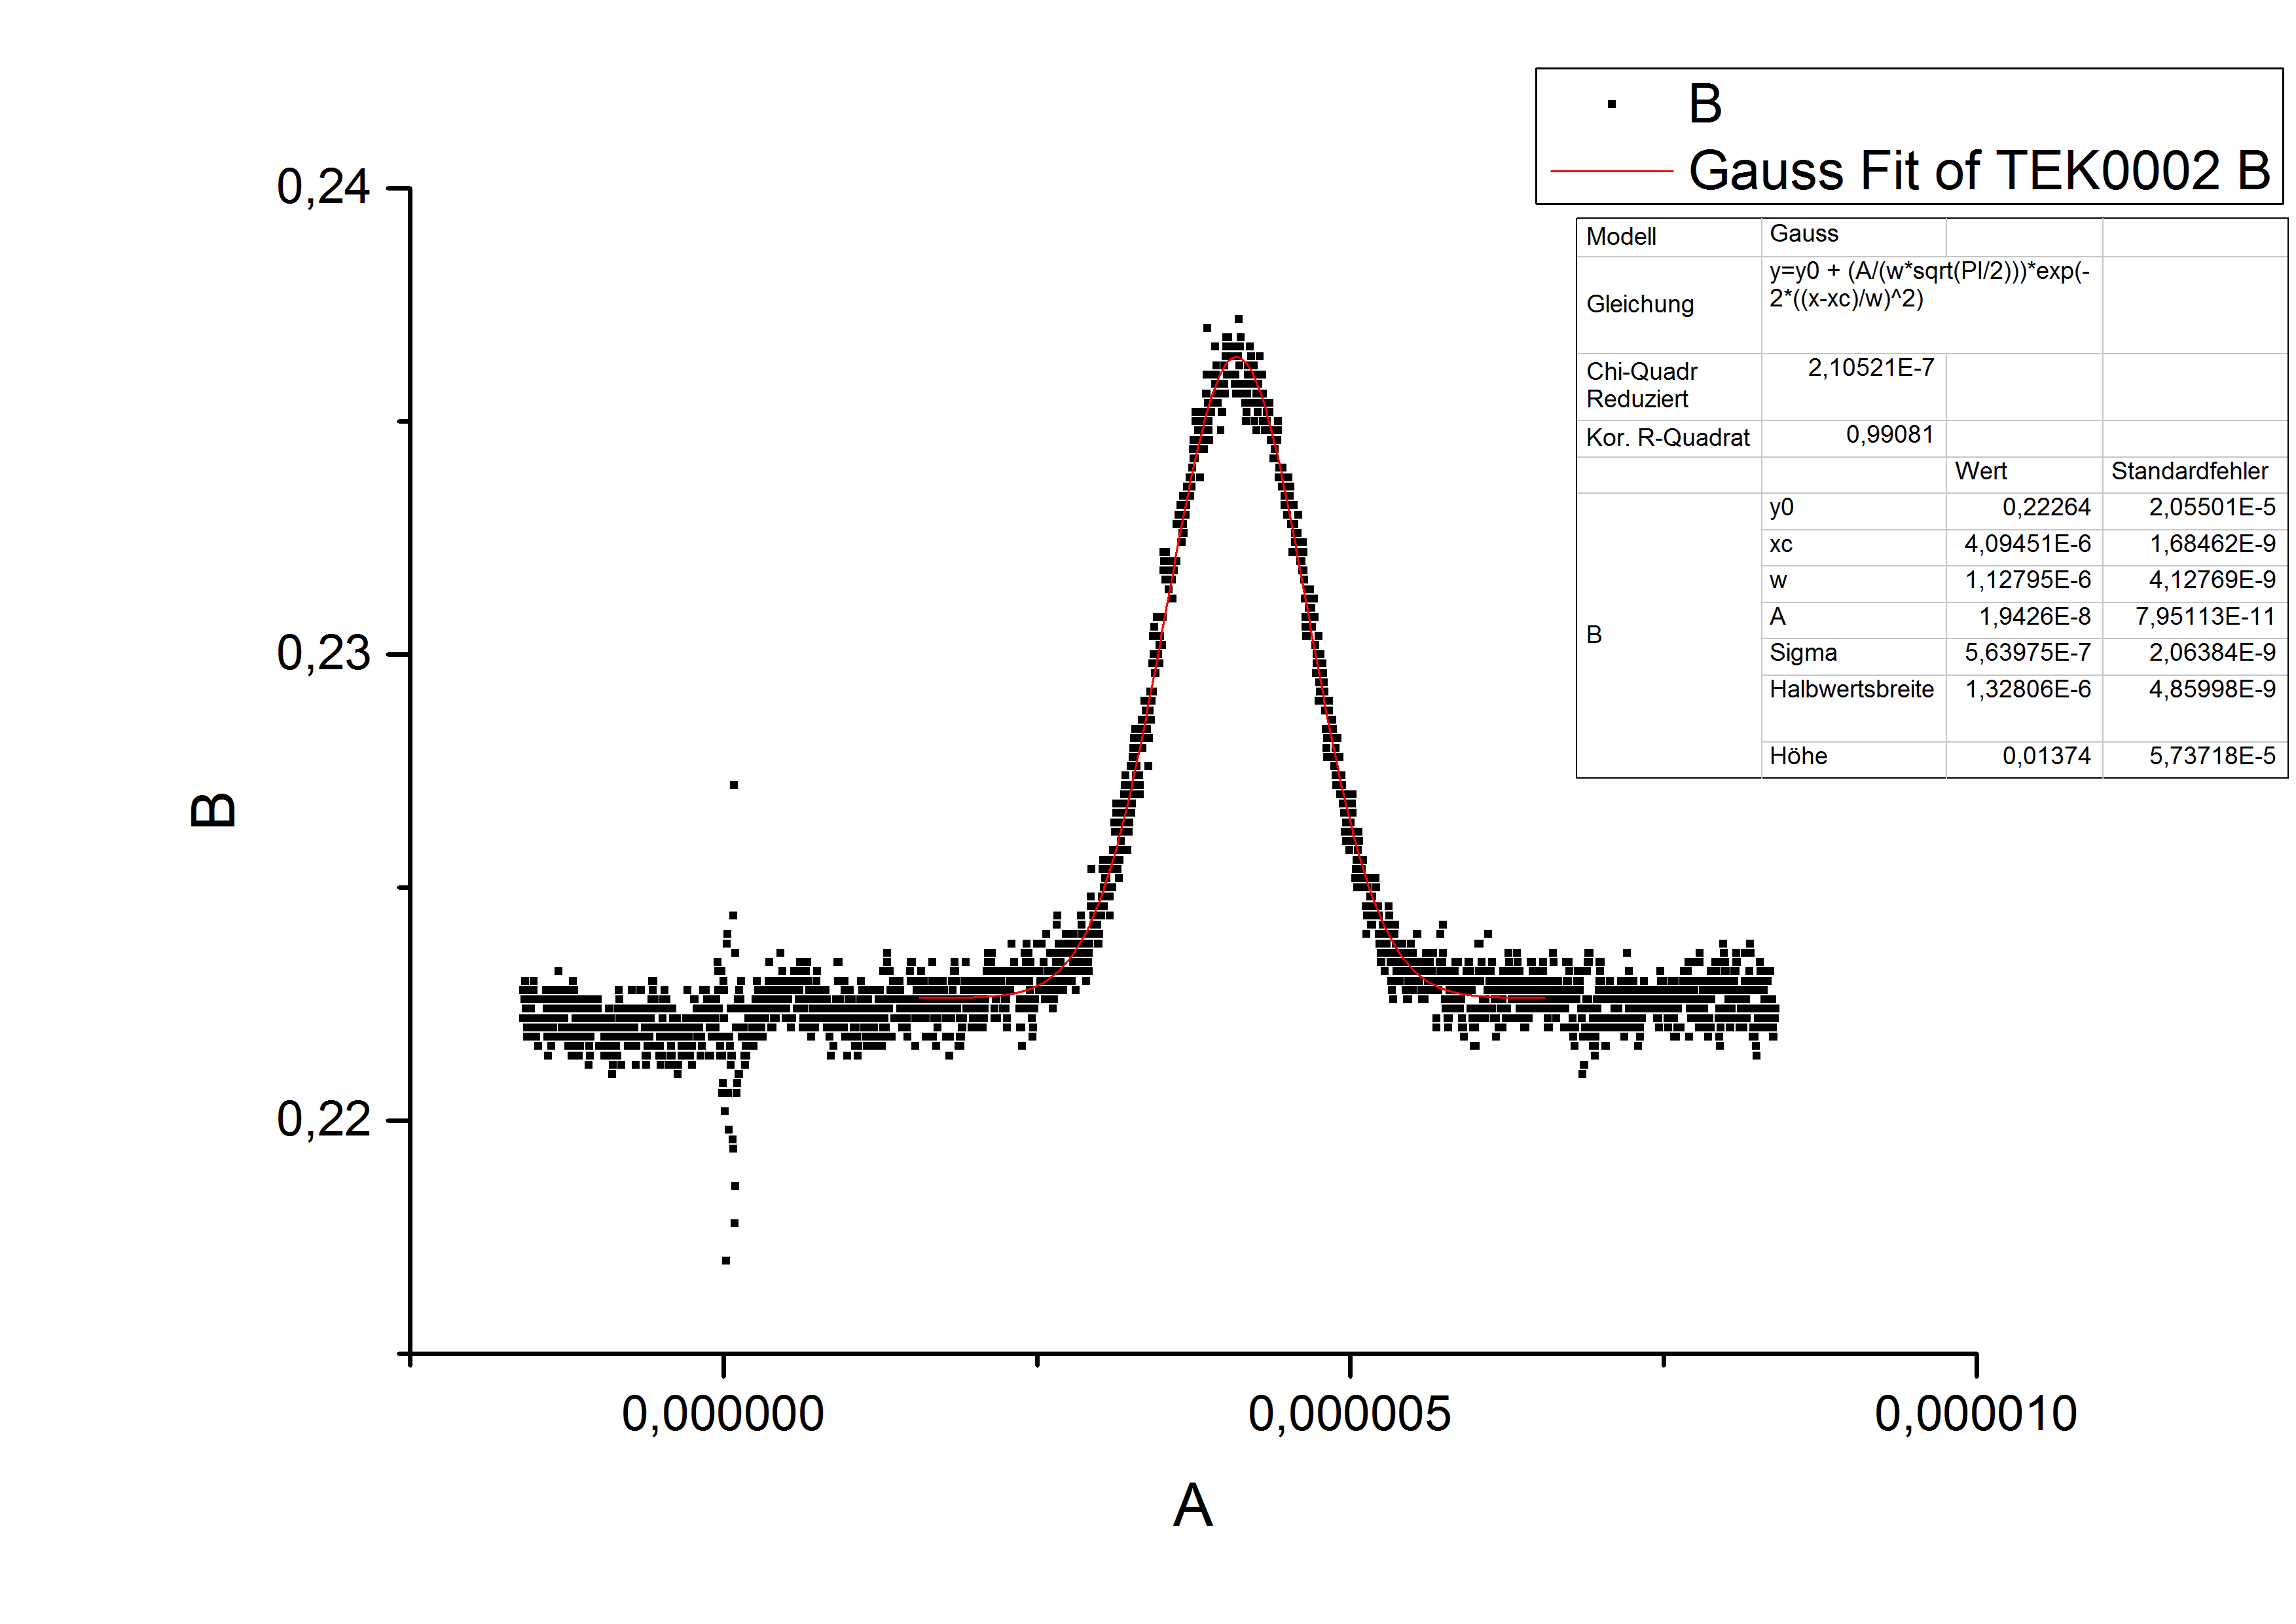
\includegraphics[scale=0.25]{Bilder/Teil2/Graph2}
\caption{Graph at 1.99mm.}
\label{fig:graph2}
\end{center}
\end{figure}
\begin{figure}[h]
\begin{center}
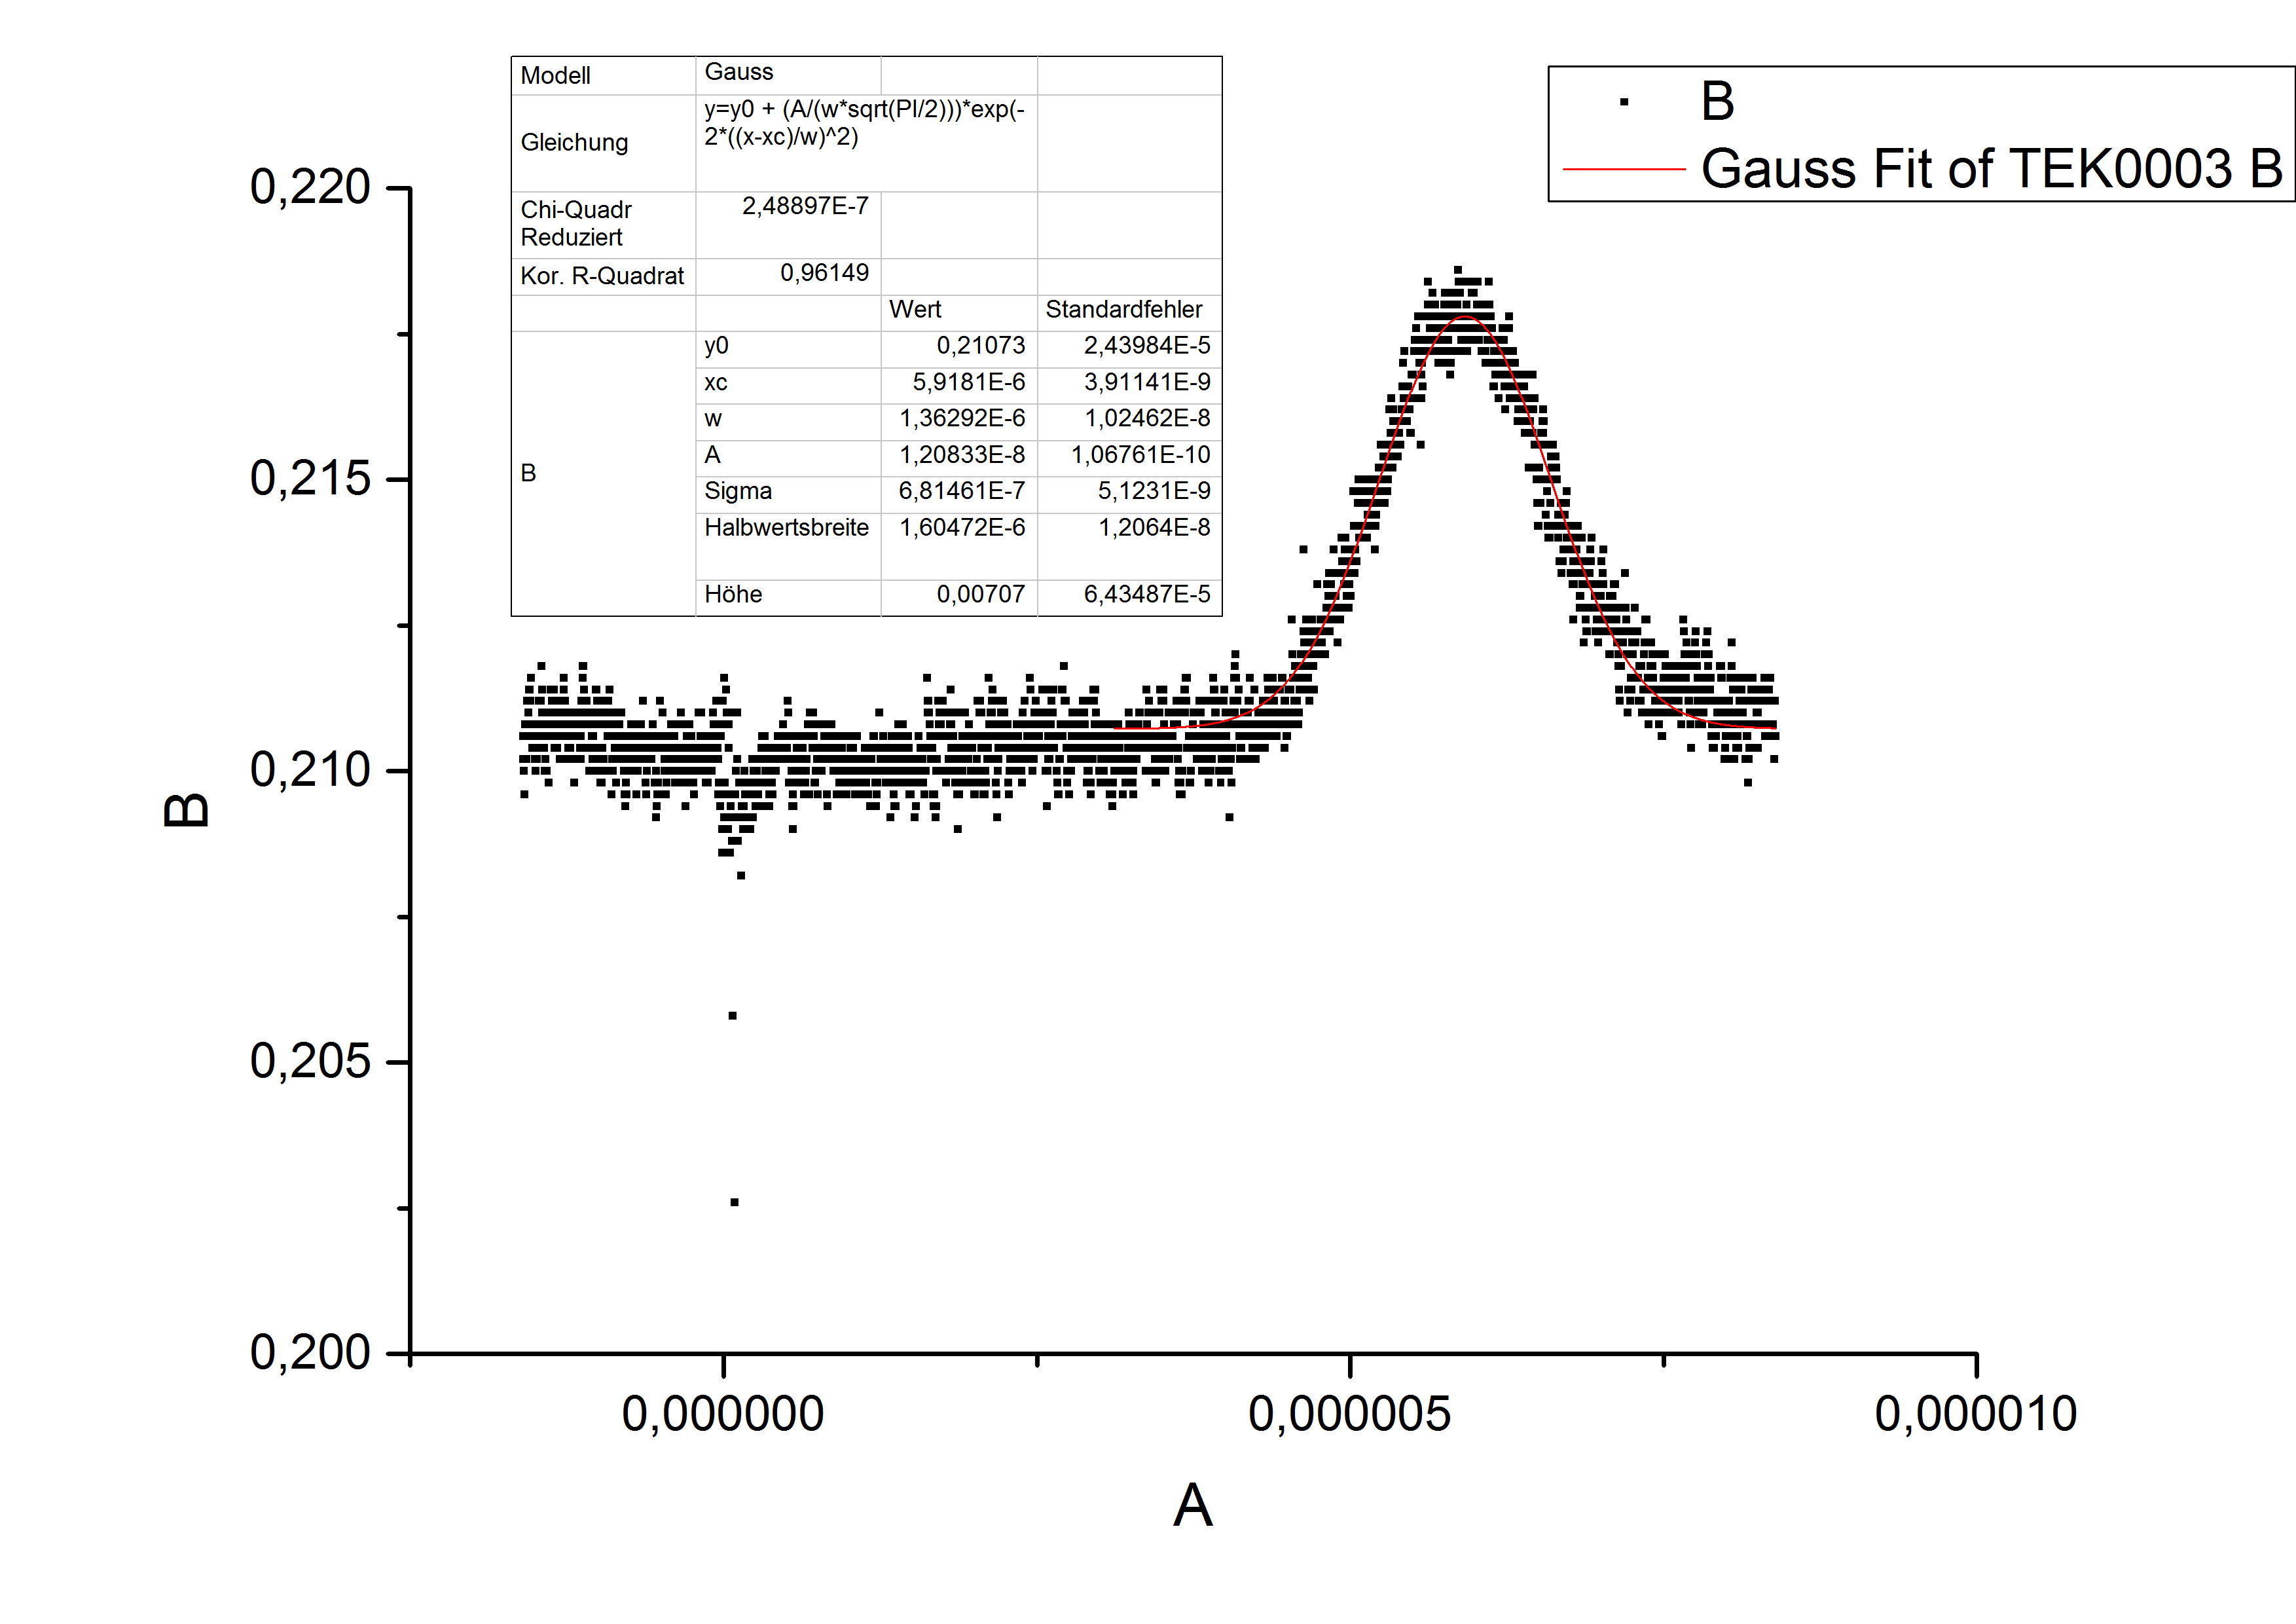
\includegraphics[scale=0.25]{Bilder/Teil2/Graph3}
\caption{Graph at 3.01mm.}
\label{fig:graph3}
\end{center}
\end{figure}
\begin{figure}[h]
\begin{center}
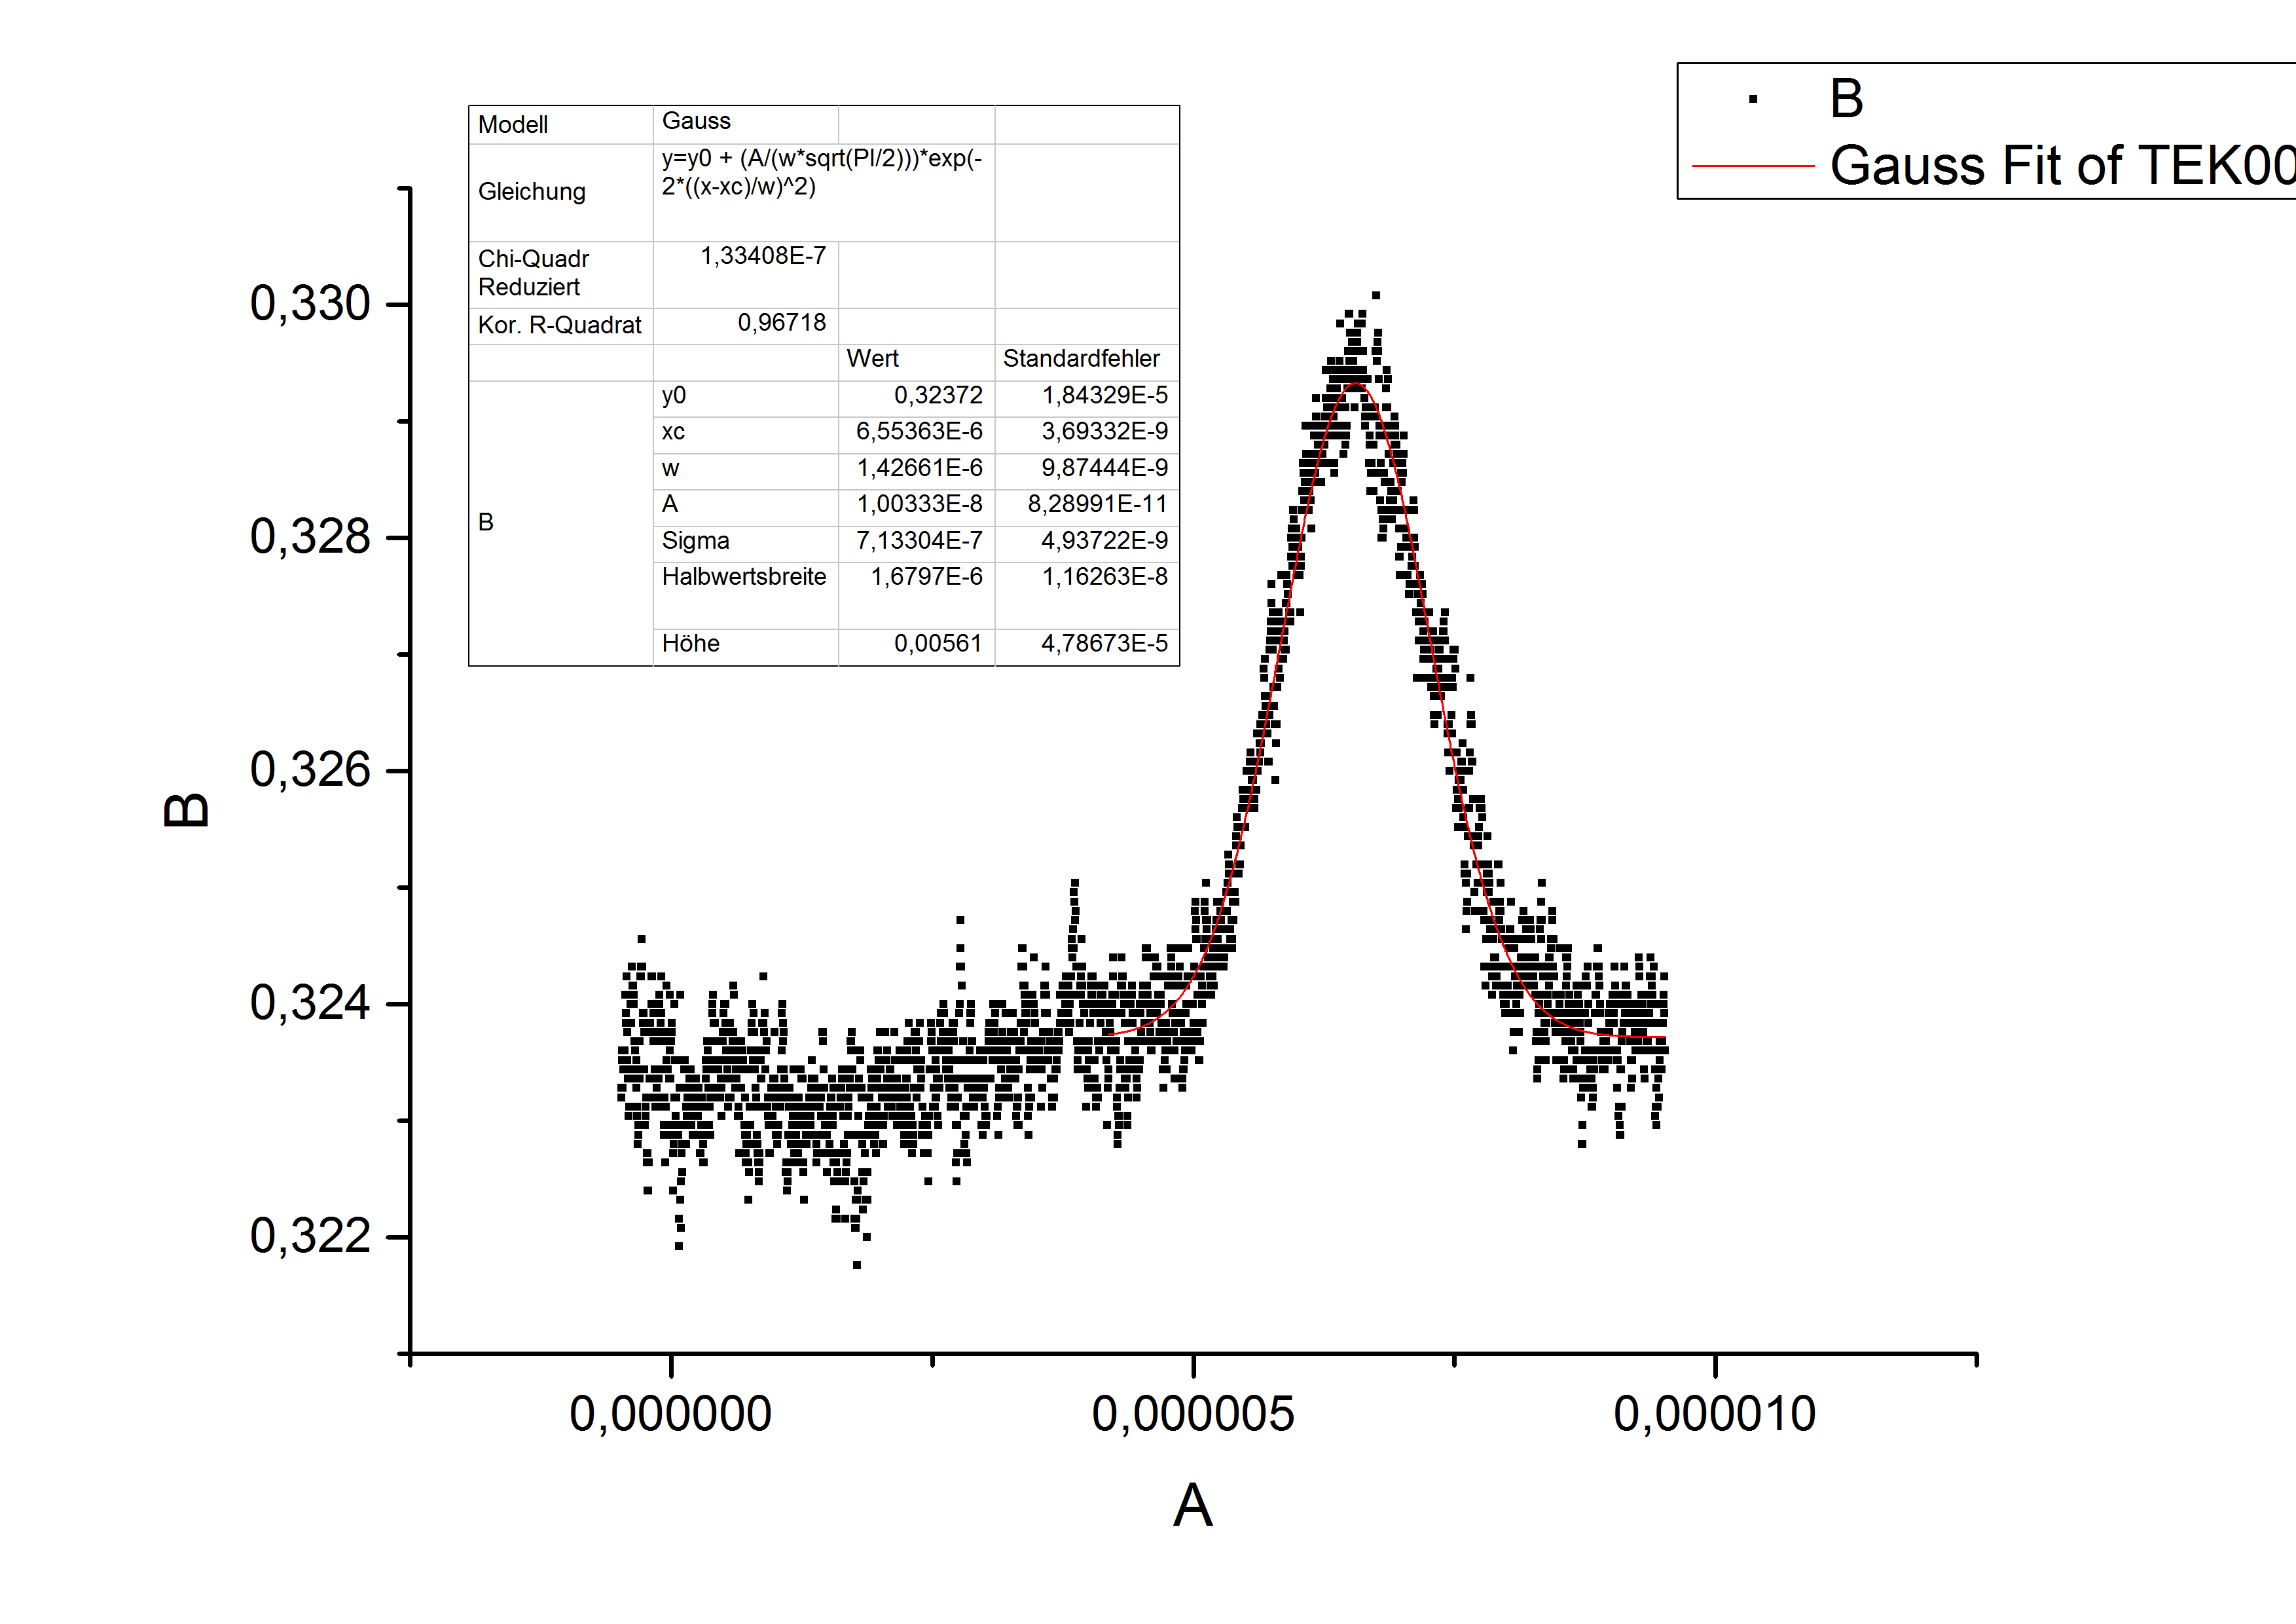
\includegraphics[scale=0.25]{Bilder/Teil2/Graph4}
\caption{Graph at 3.55mm.}
\label{fig:graph4}
\end{center}
\end{figure}
\begin{figure}[h]
\begin{center}
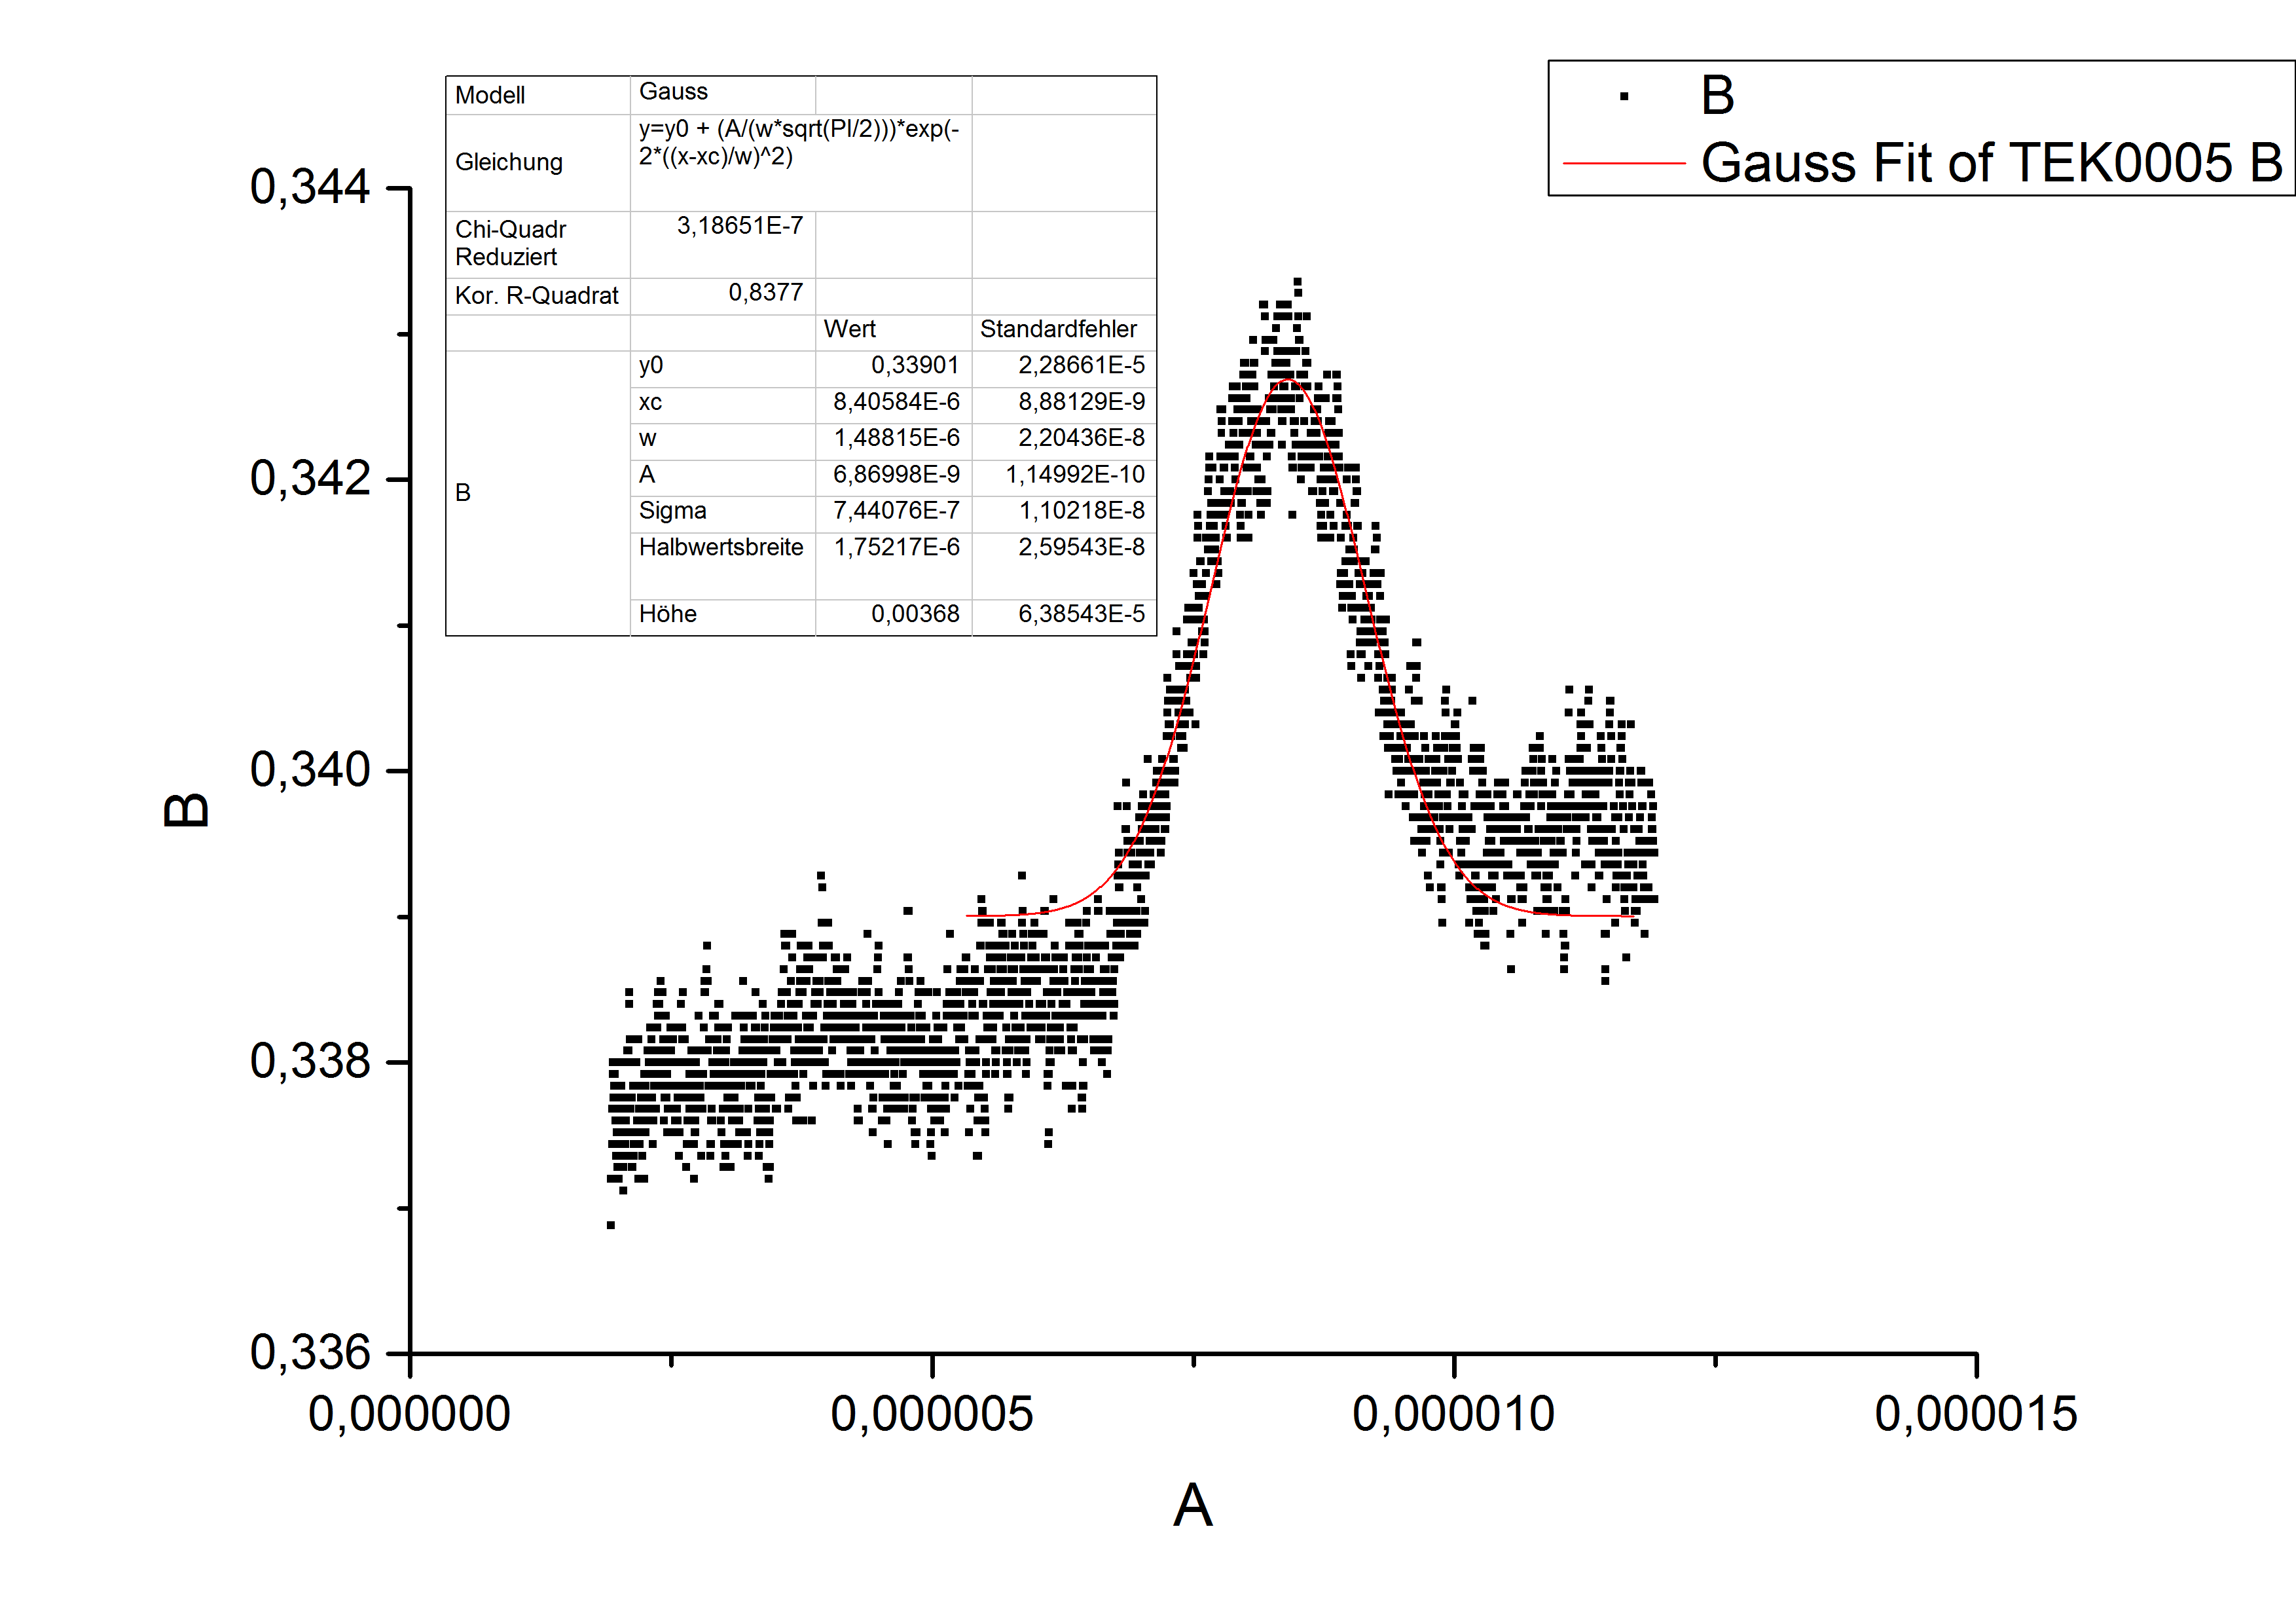
\includegraphics[scale=0.25]{Bilder/Teil2/Graph5}
\caption{Graph at 4.01mm.}
\label{fig:graph5}
\end{center}
\end{figure}
\begin{figure}[h]
\begin{center}
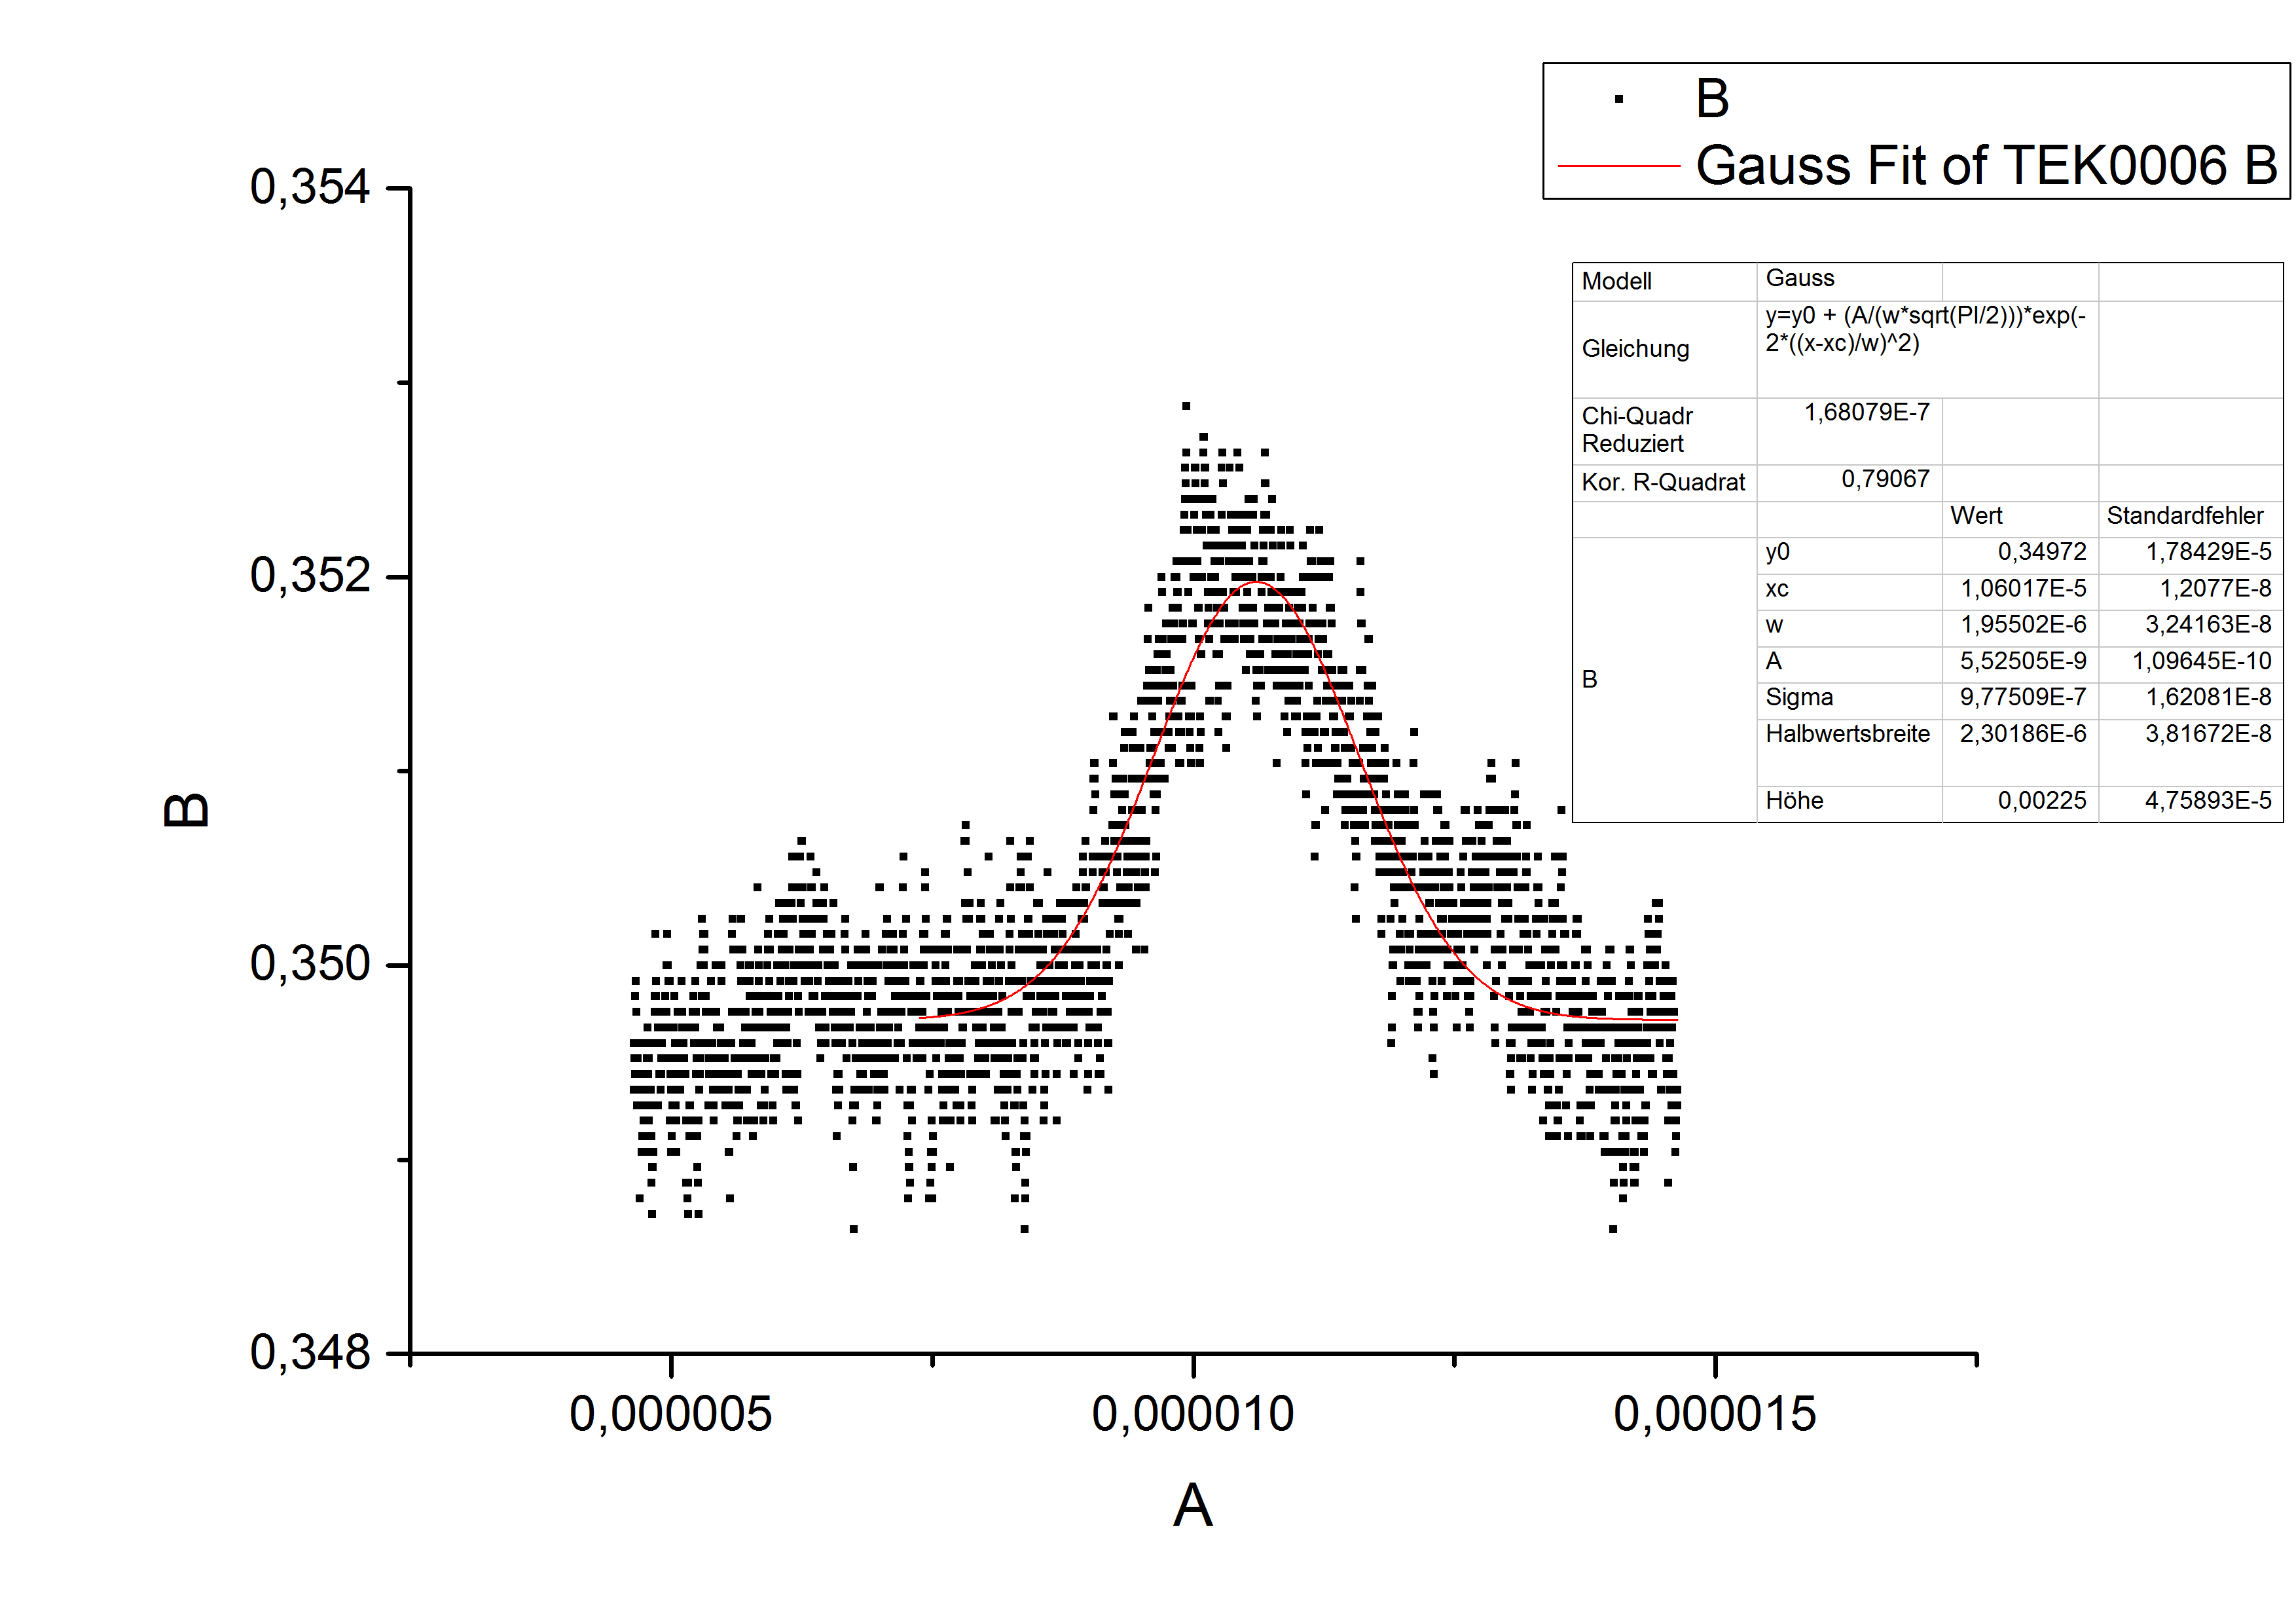
\includegraphics[scale=0.25]{Bilder/Teil2/Graph6}
\caption{Graph at 4.53mm.}
\label{fig:graph6}
\end{center}
\end{figure}
\begin{figure}[h]
\begin{center}
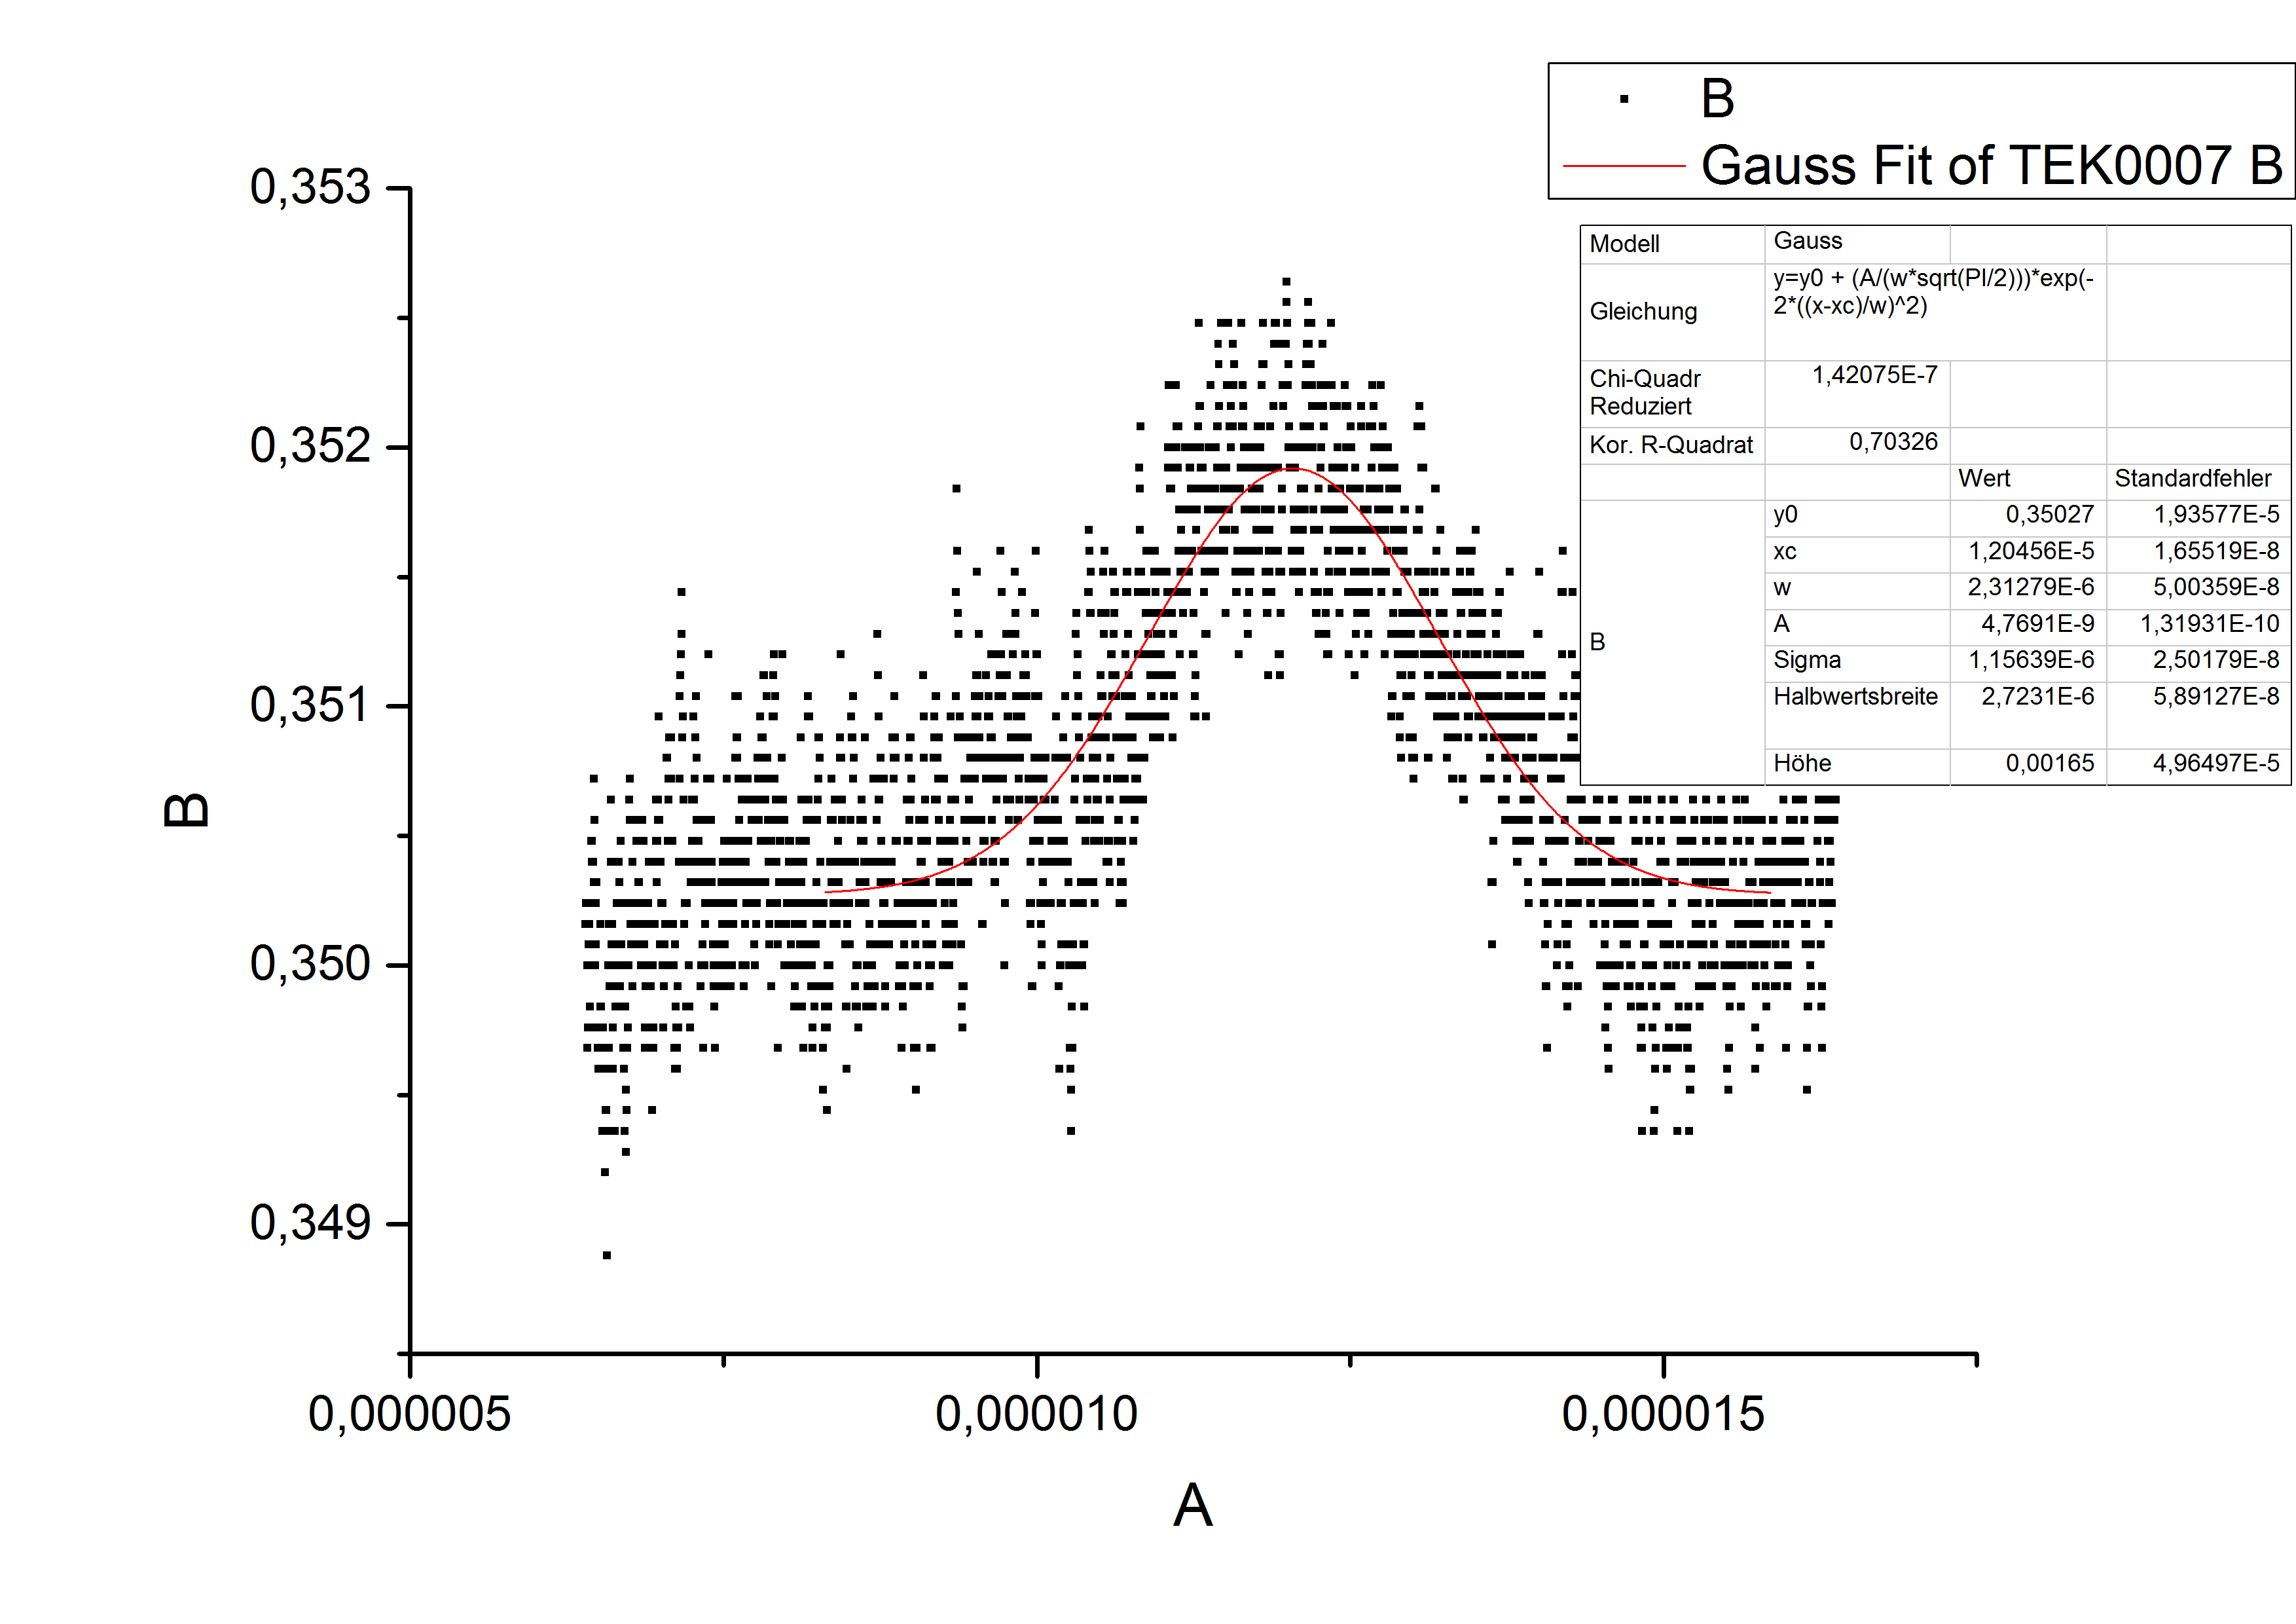
\includegraphics[scale=0.25]{Bilder/Teil2/Graph7}
\caption{Graph at 5.05mm.}
\label{fig:graph7}
\end{center}
\end{figure}
\begin{figure}[h]
\begin{center}
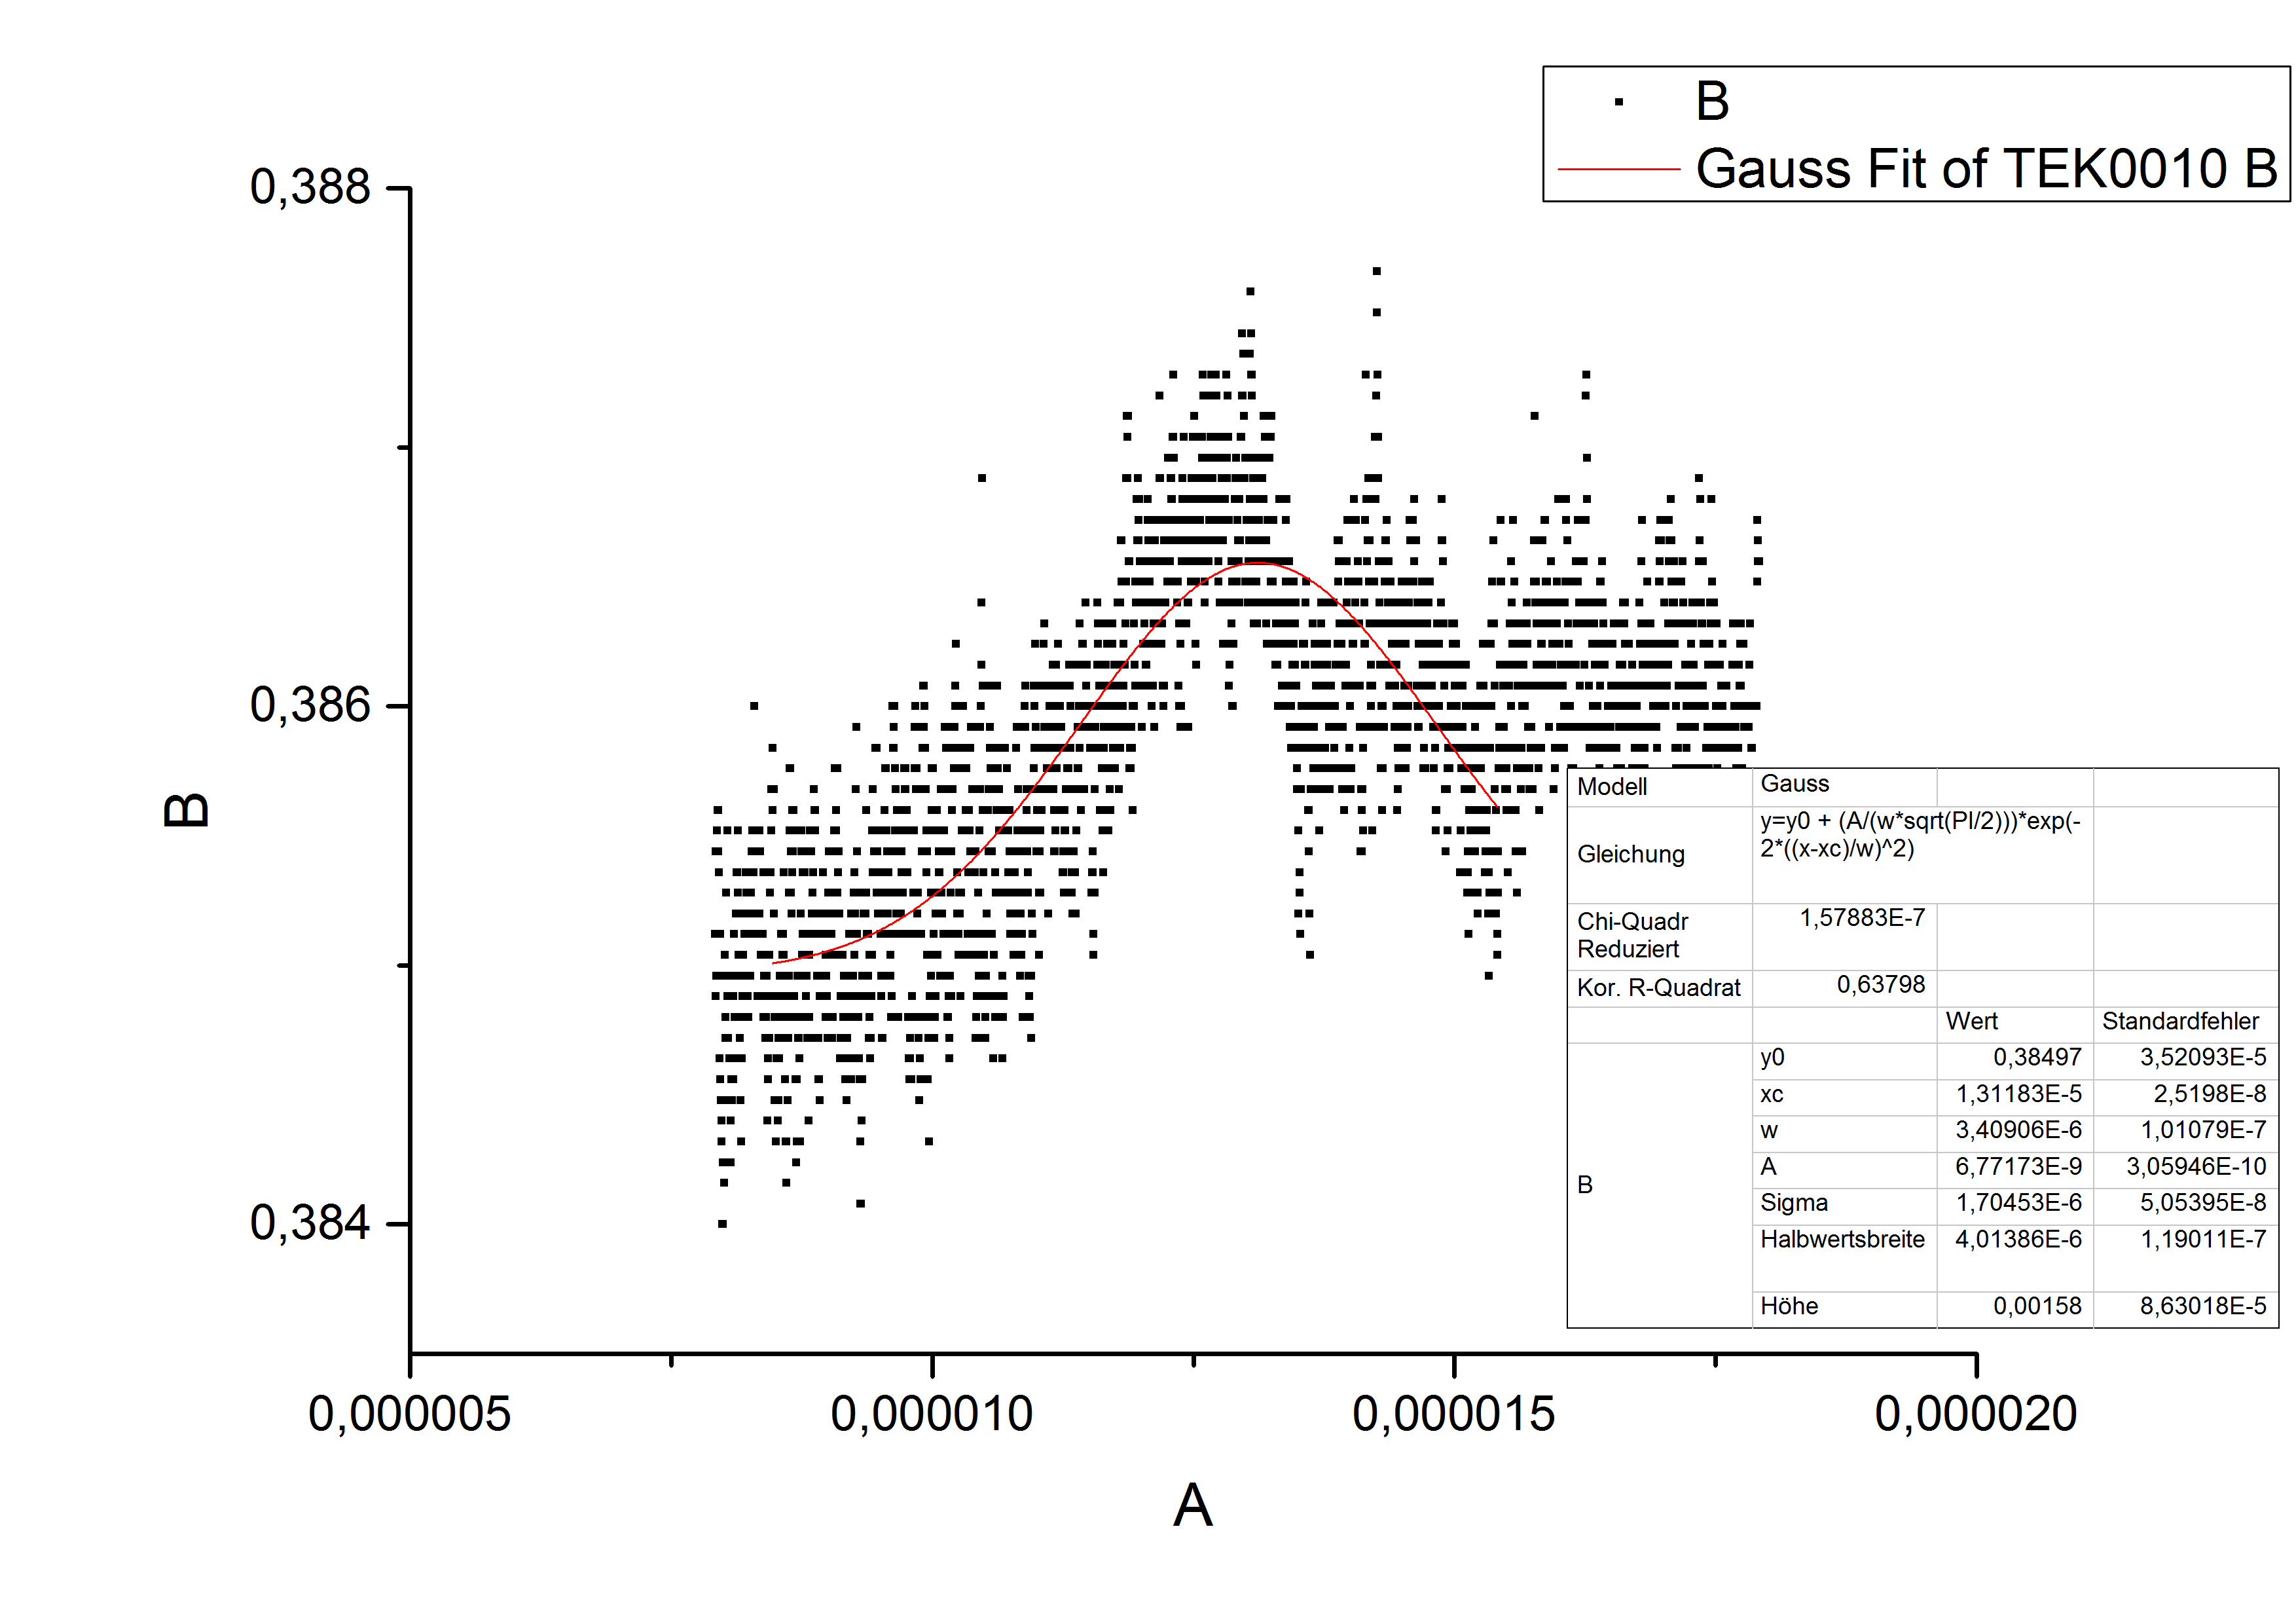
\includegraphics[scale=0.25]{Bilder/Teil2/Graph8}
\caption{Graph at 55.52mm.}
\label{fig:graph8}
\end{center}
\end{figure}
\begin{figure}[h]
\begin{center}
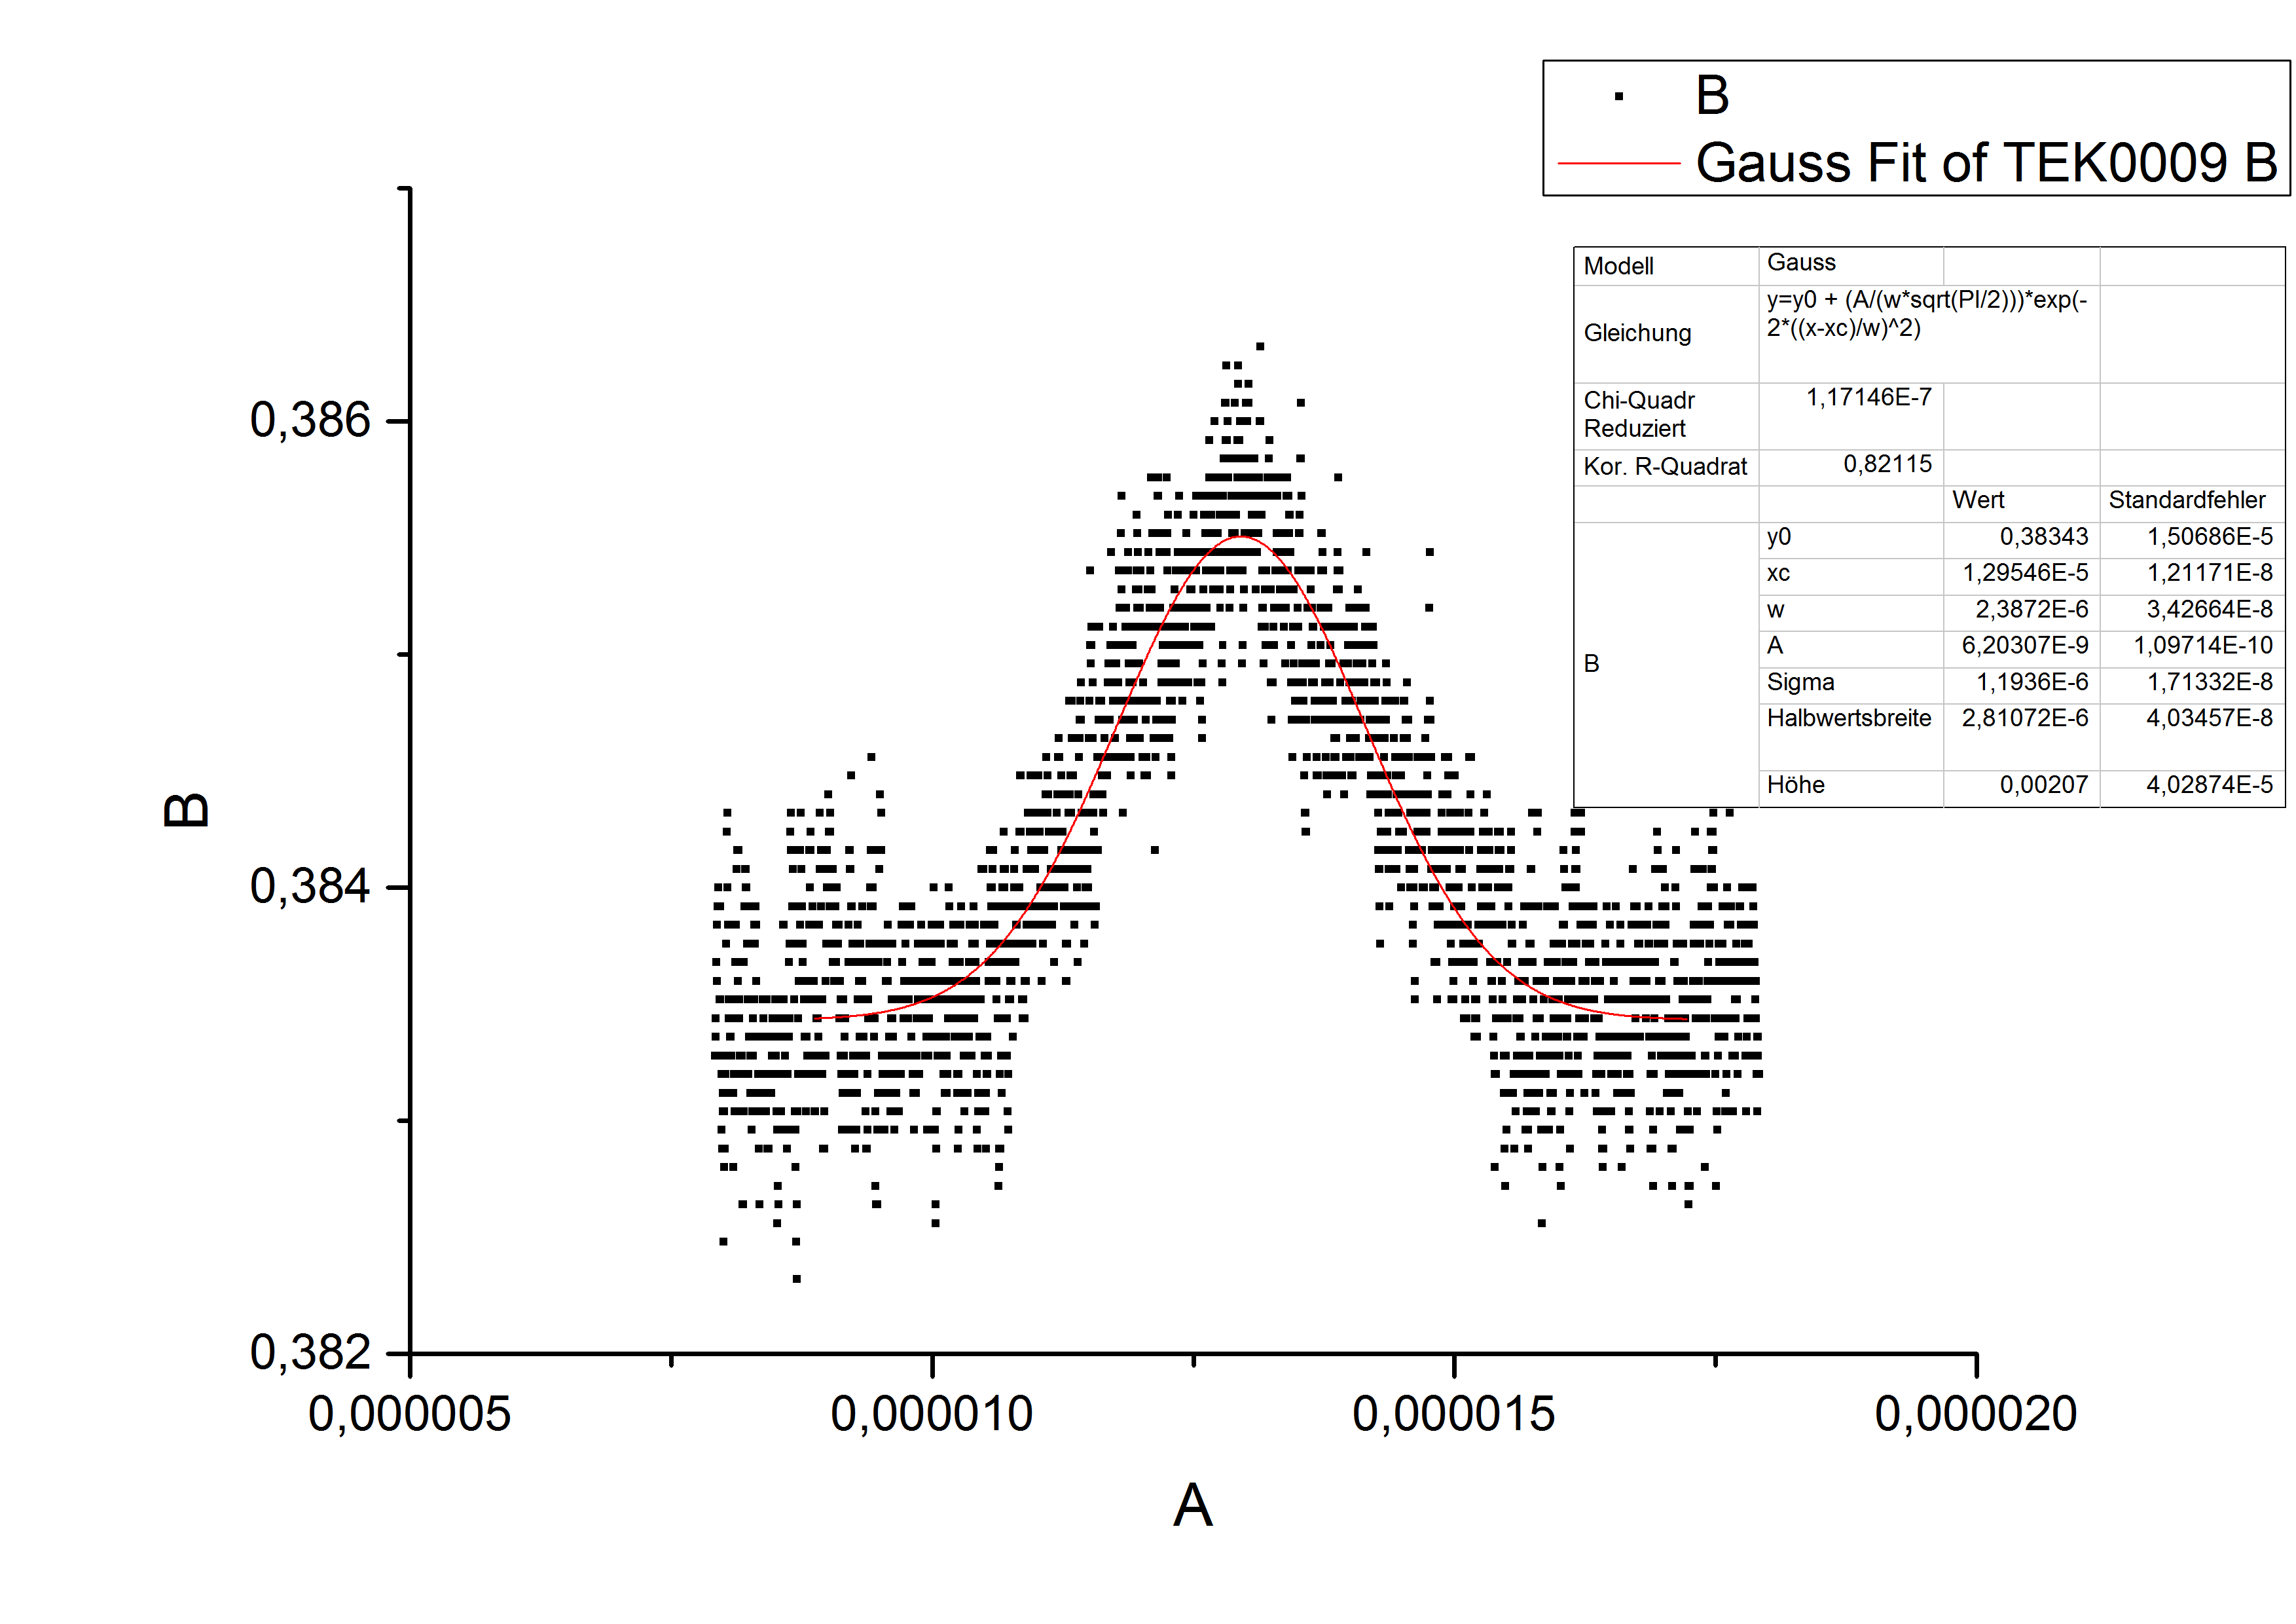
\includegraphics[scale=0.25]{Bilder/Teil2/Graph9}
\caption{Graph at 6.02mm.}
\label{fig:graph9}
\end{center}
\end{figure}
\begin{figure}[h]
\begin{center}
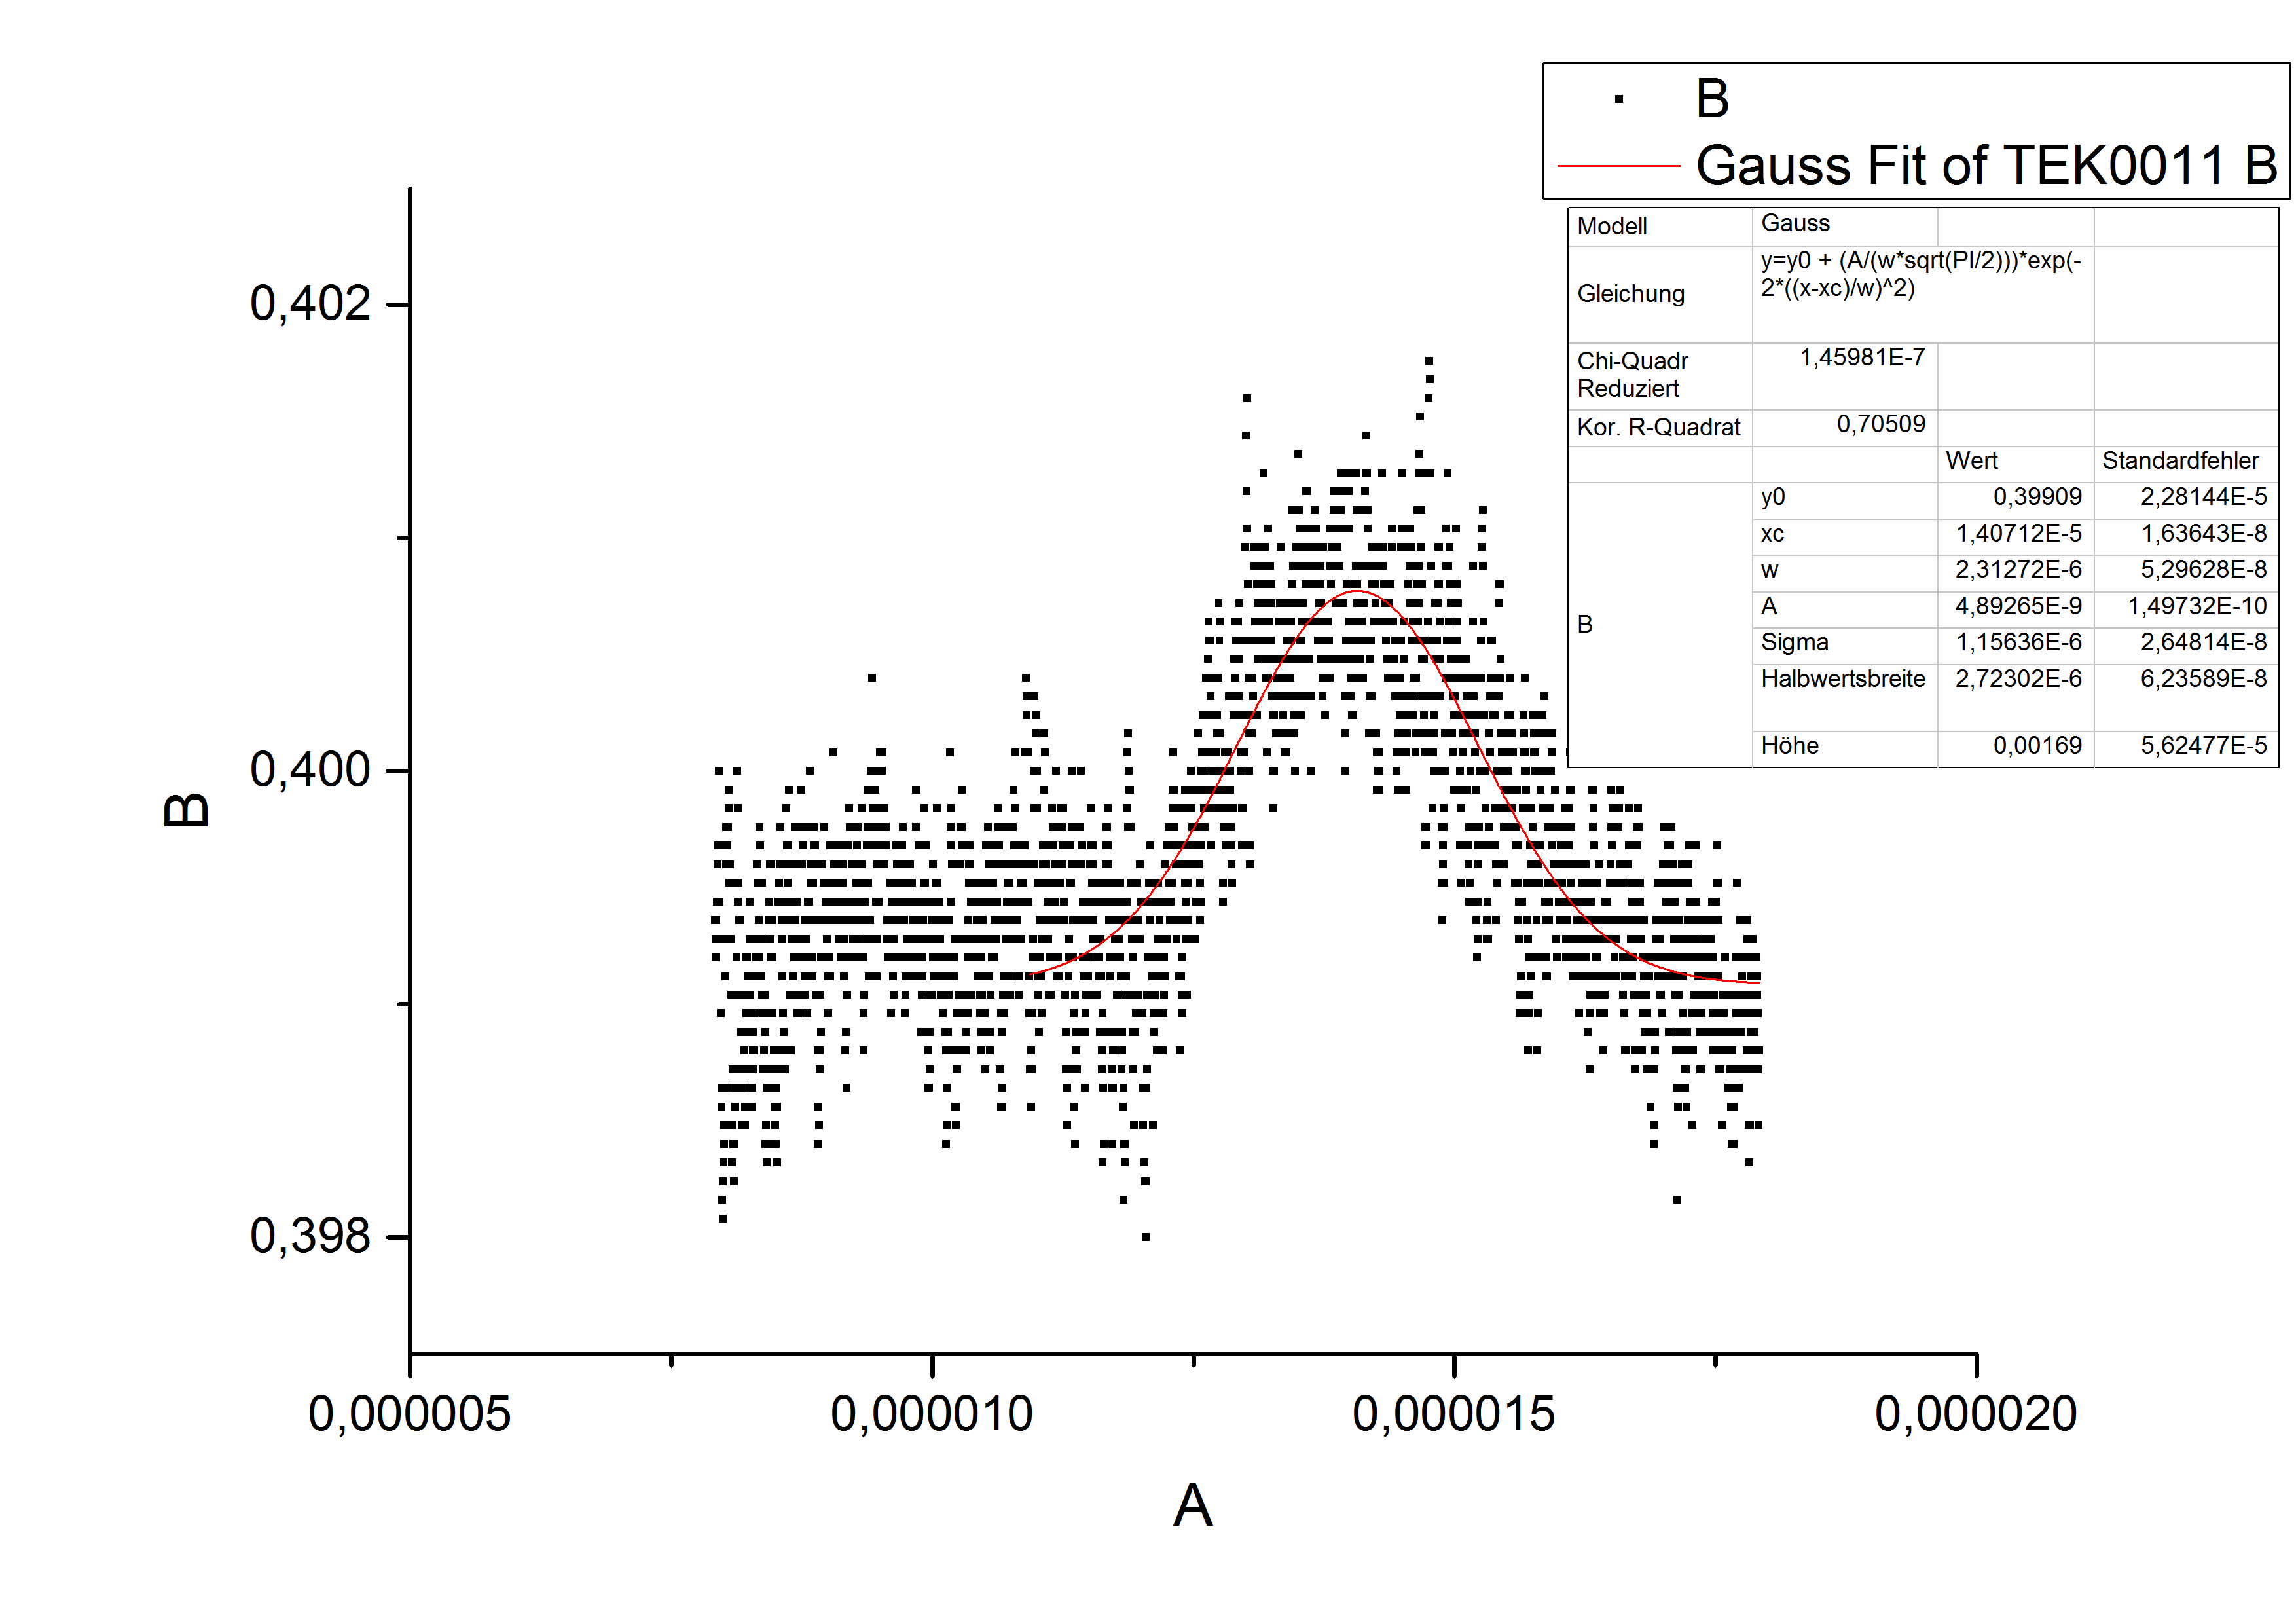
\includegraphics[scale=0.25]{Bilder/Teil2/Graph10}
\caption{Graph at 6.58mm.}
\label{fig:graph10}
\end{center}
\end{figure}
\begin{figure}[h]
\begin{center}
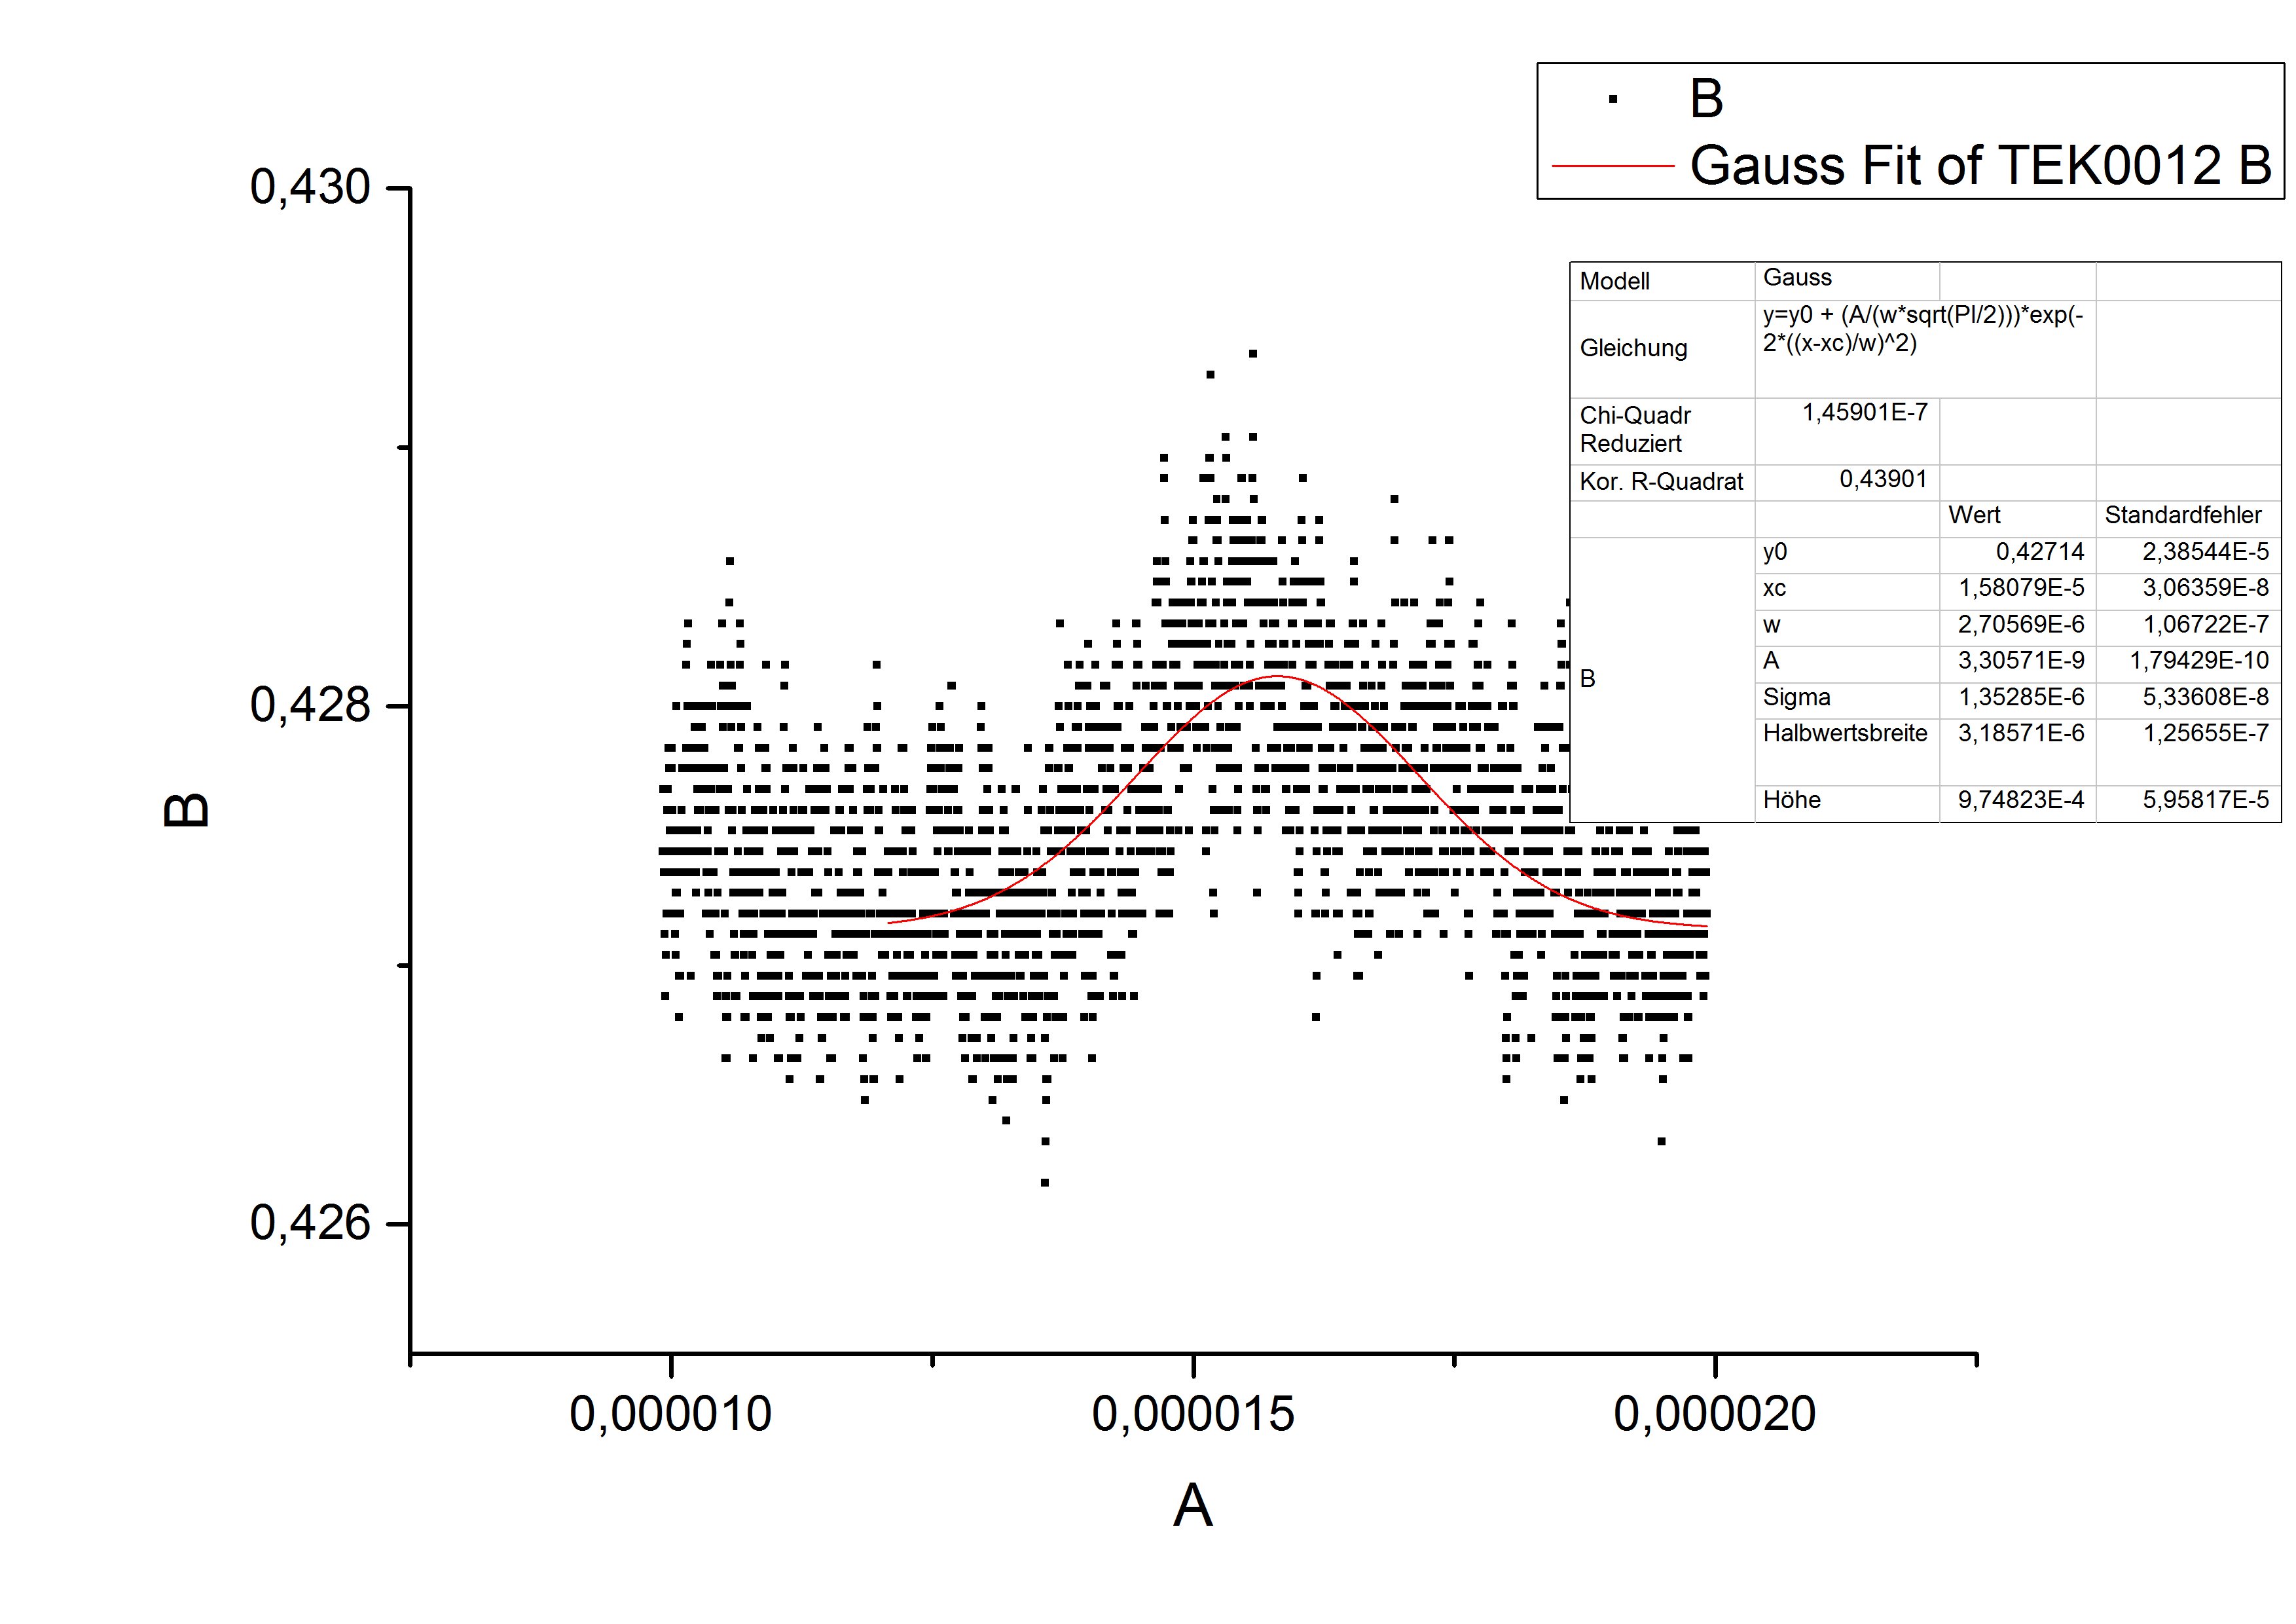
\includegraphics[scale=0.25]{Bilder/Teil2/Graph11}
\caption{Graph at 7.02mm.}
\label{fig:graph11}
\end{center}
\end{figure}
\begin{figure}[h]
\begin{center}
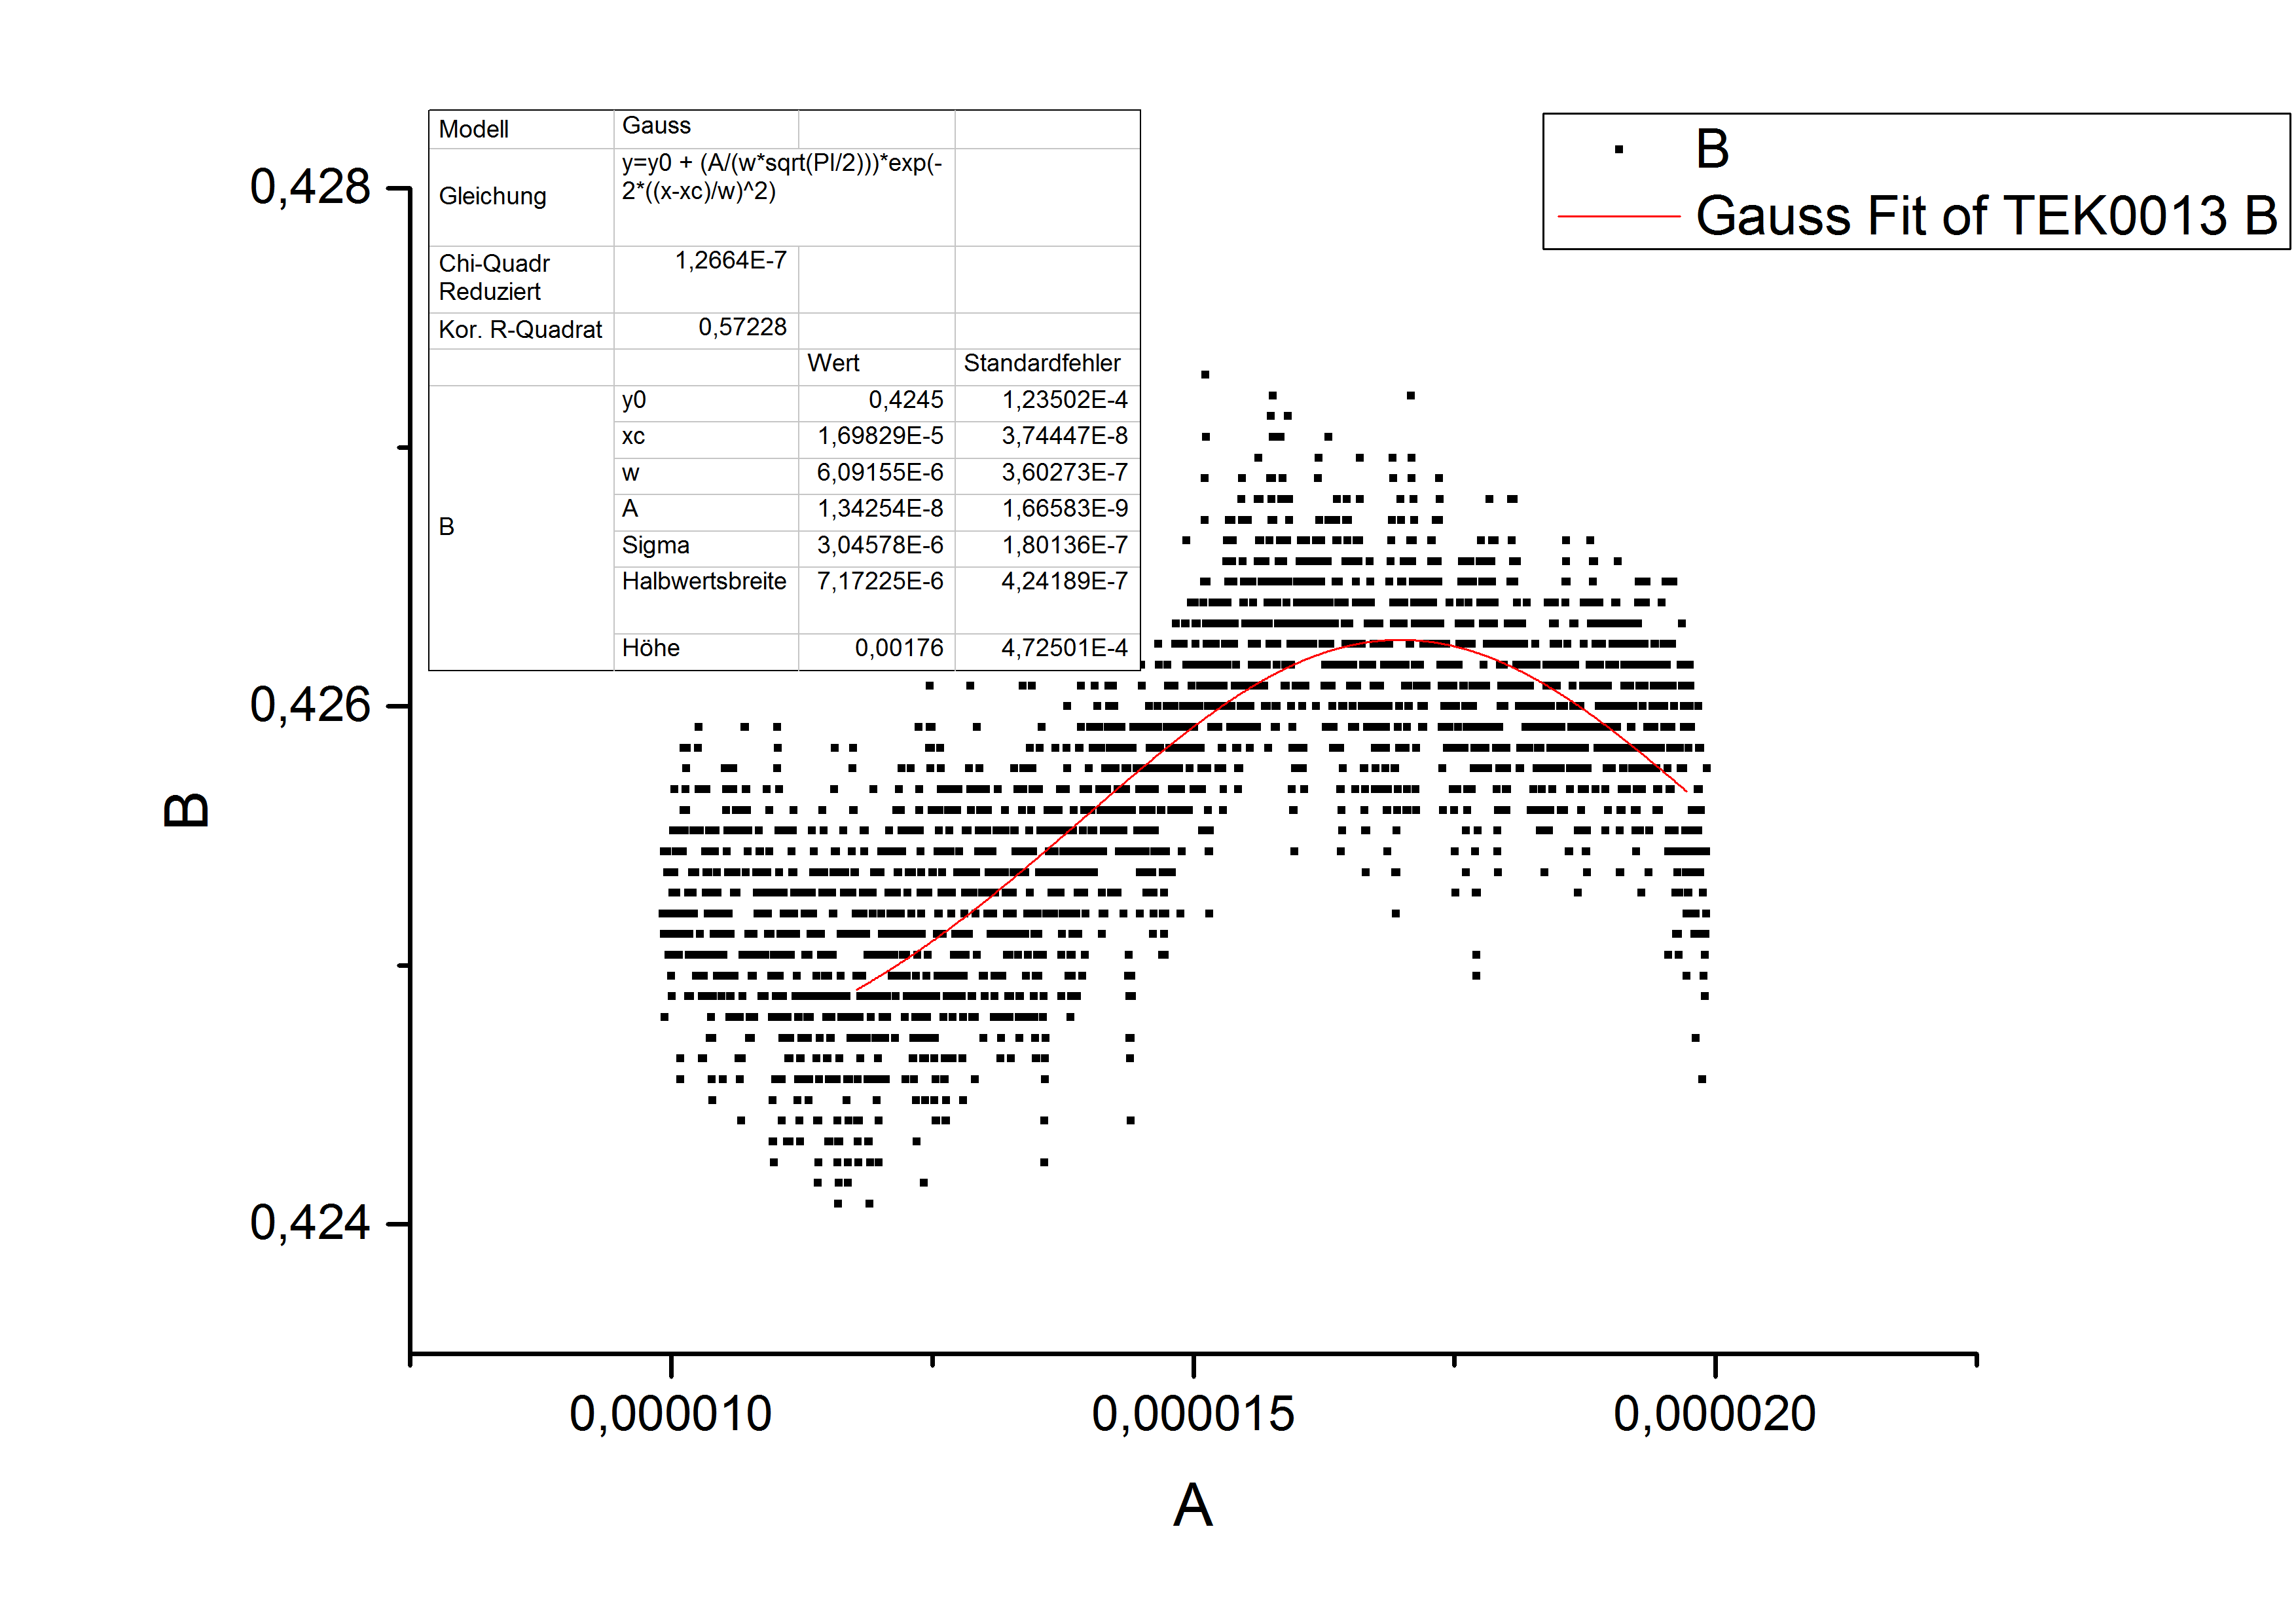
\includegraphics[scale=0.25]{Bilder/Teil2/Graph12}
\caption{Graph at 7.59mm.}
\label{fig:graph12}
\end{center}
\end{figure}
\newpage
\subsection*{Second series of measurements}
\begin{figure}[h]
\begin{center}
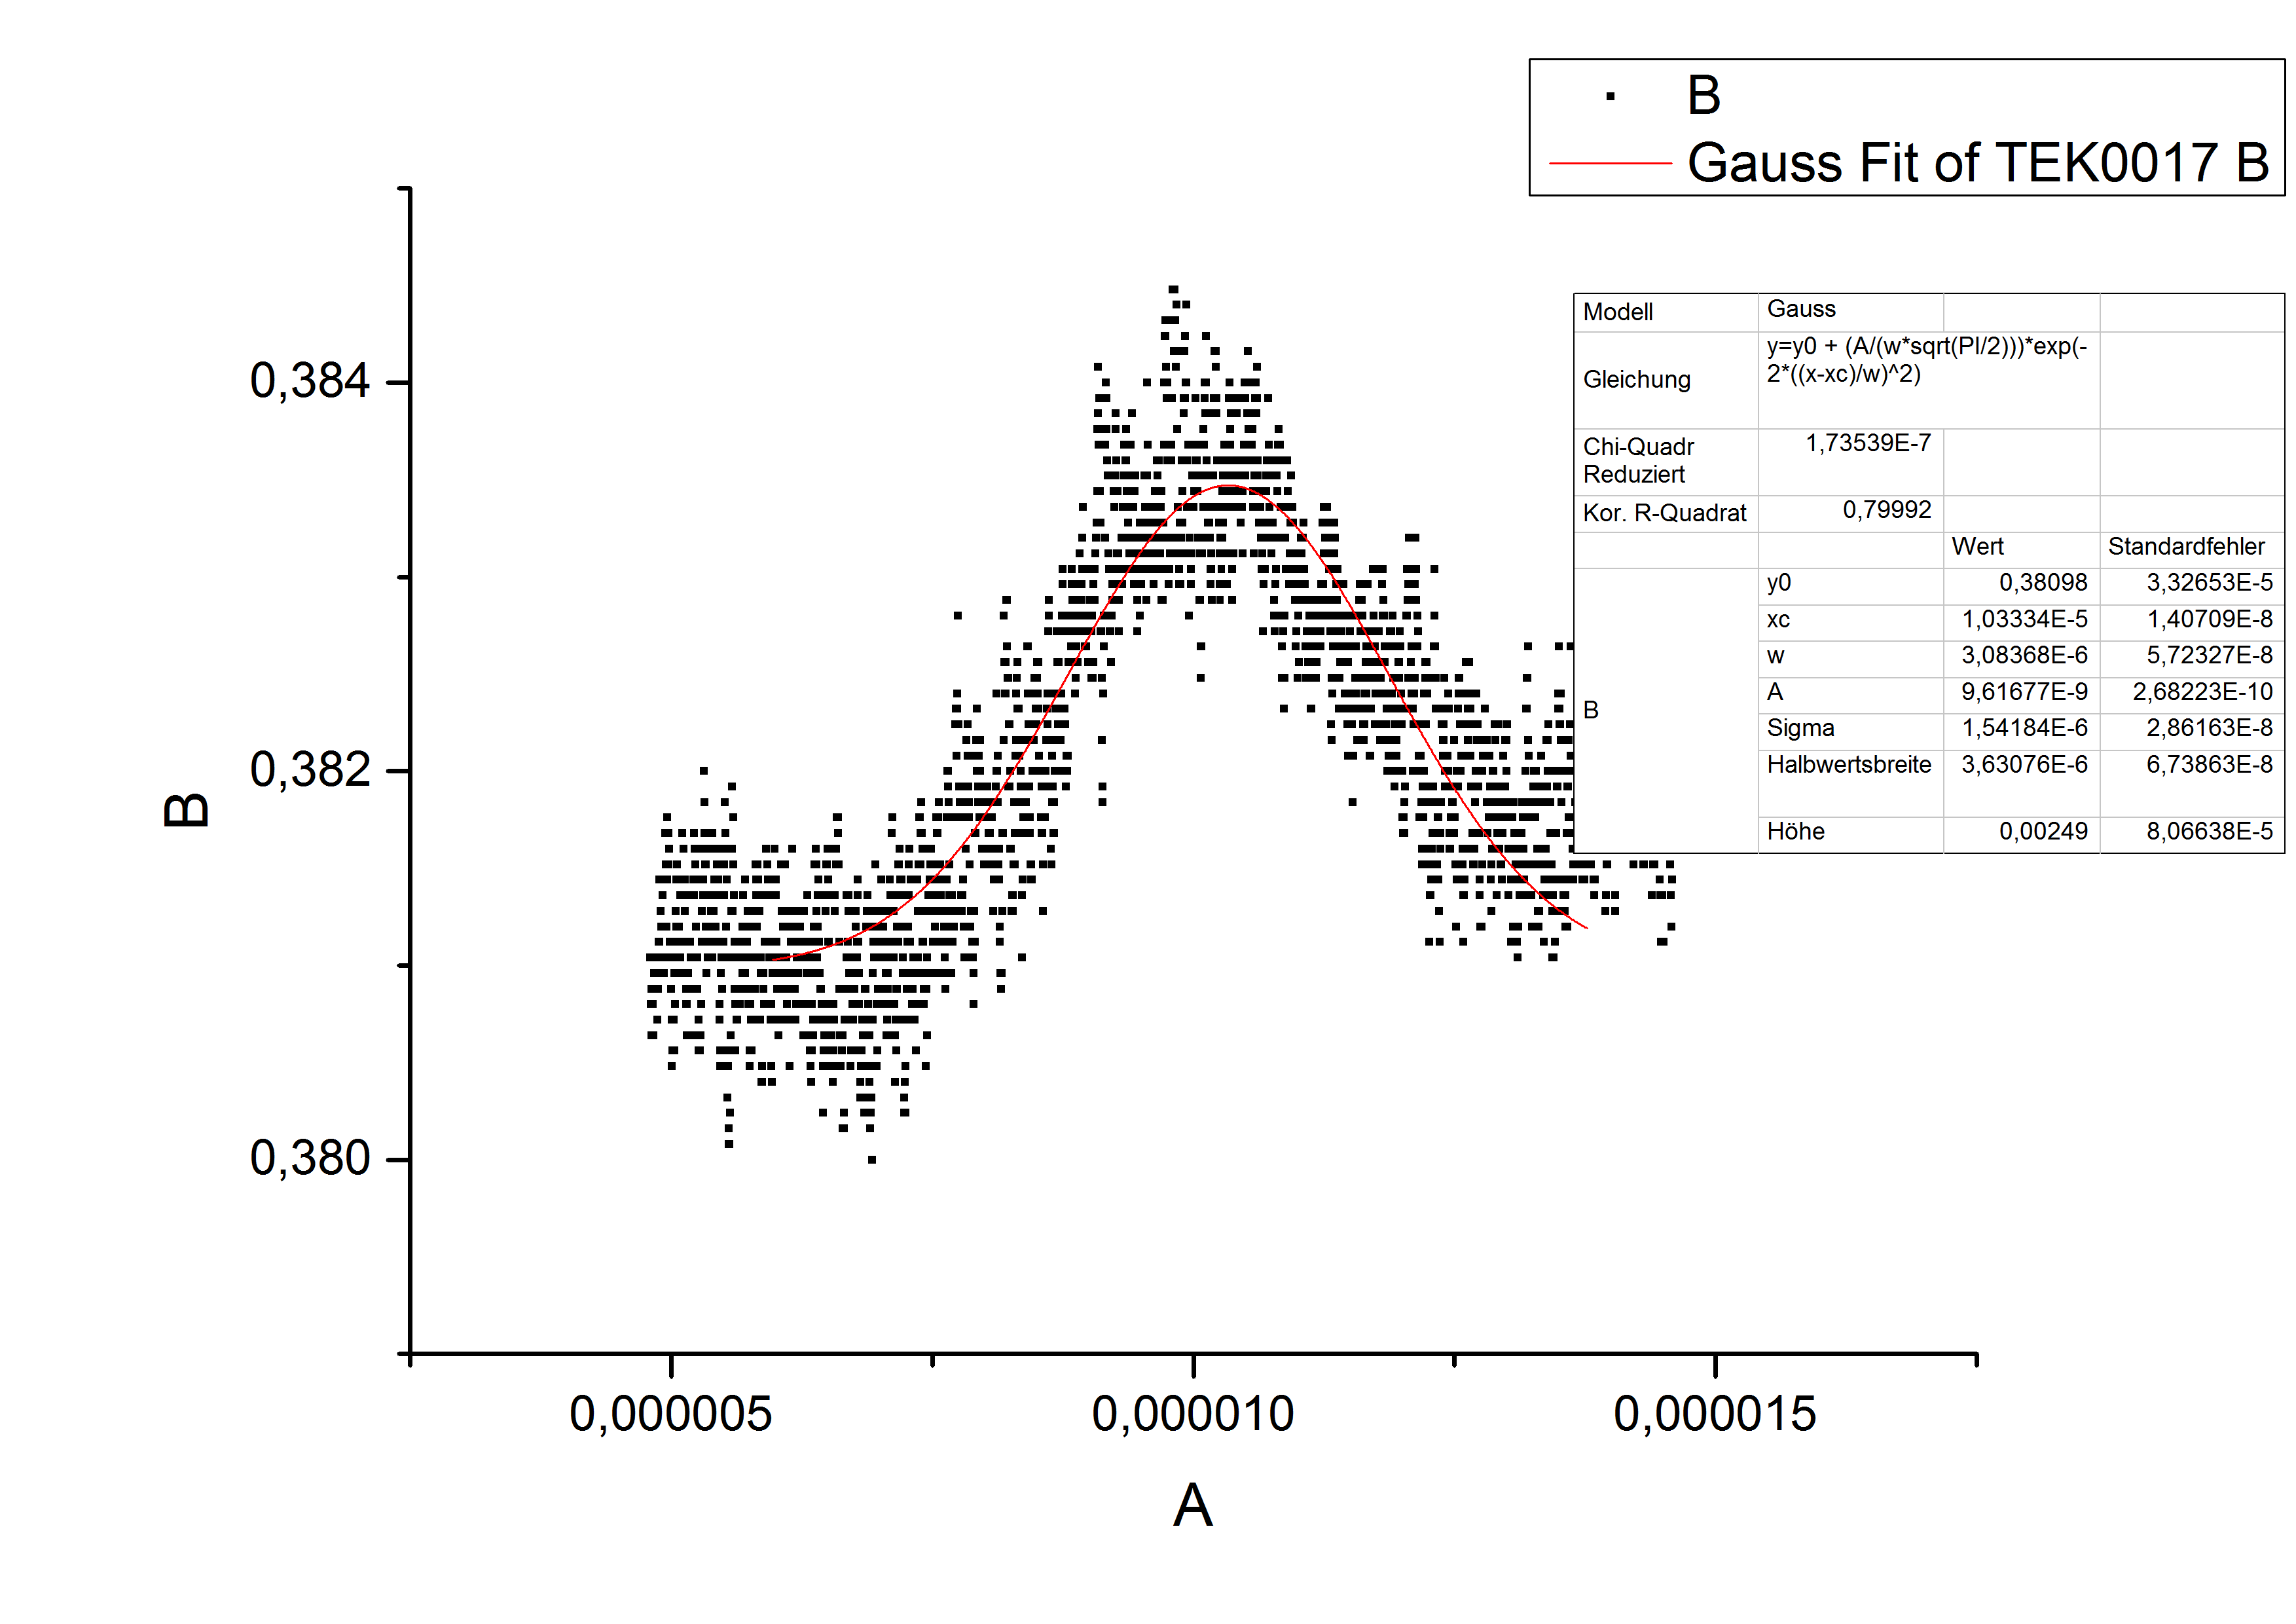
\includegraphics[scale=0.25]{Bilder/Teil2/21}
\caption{Graph at 50V.}
\label{fig:21}
\end{center}
\end{figure}
\begin{figure}[h]
\begin{center}
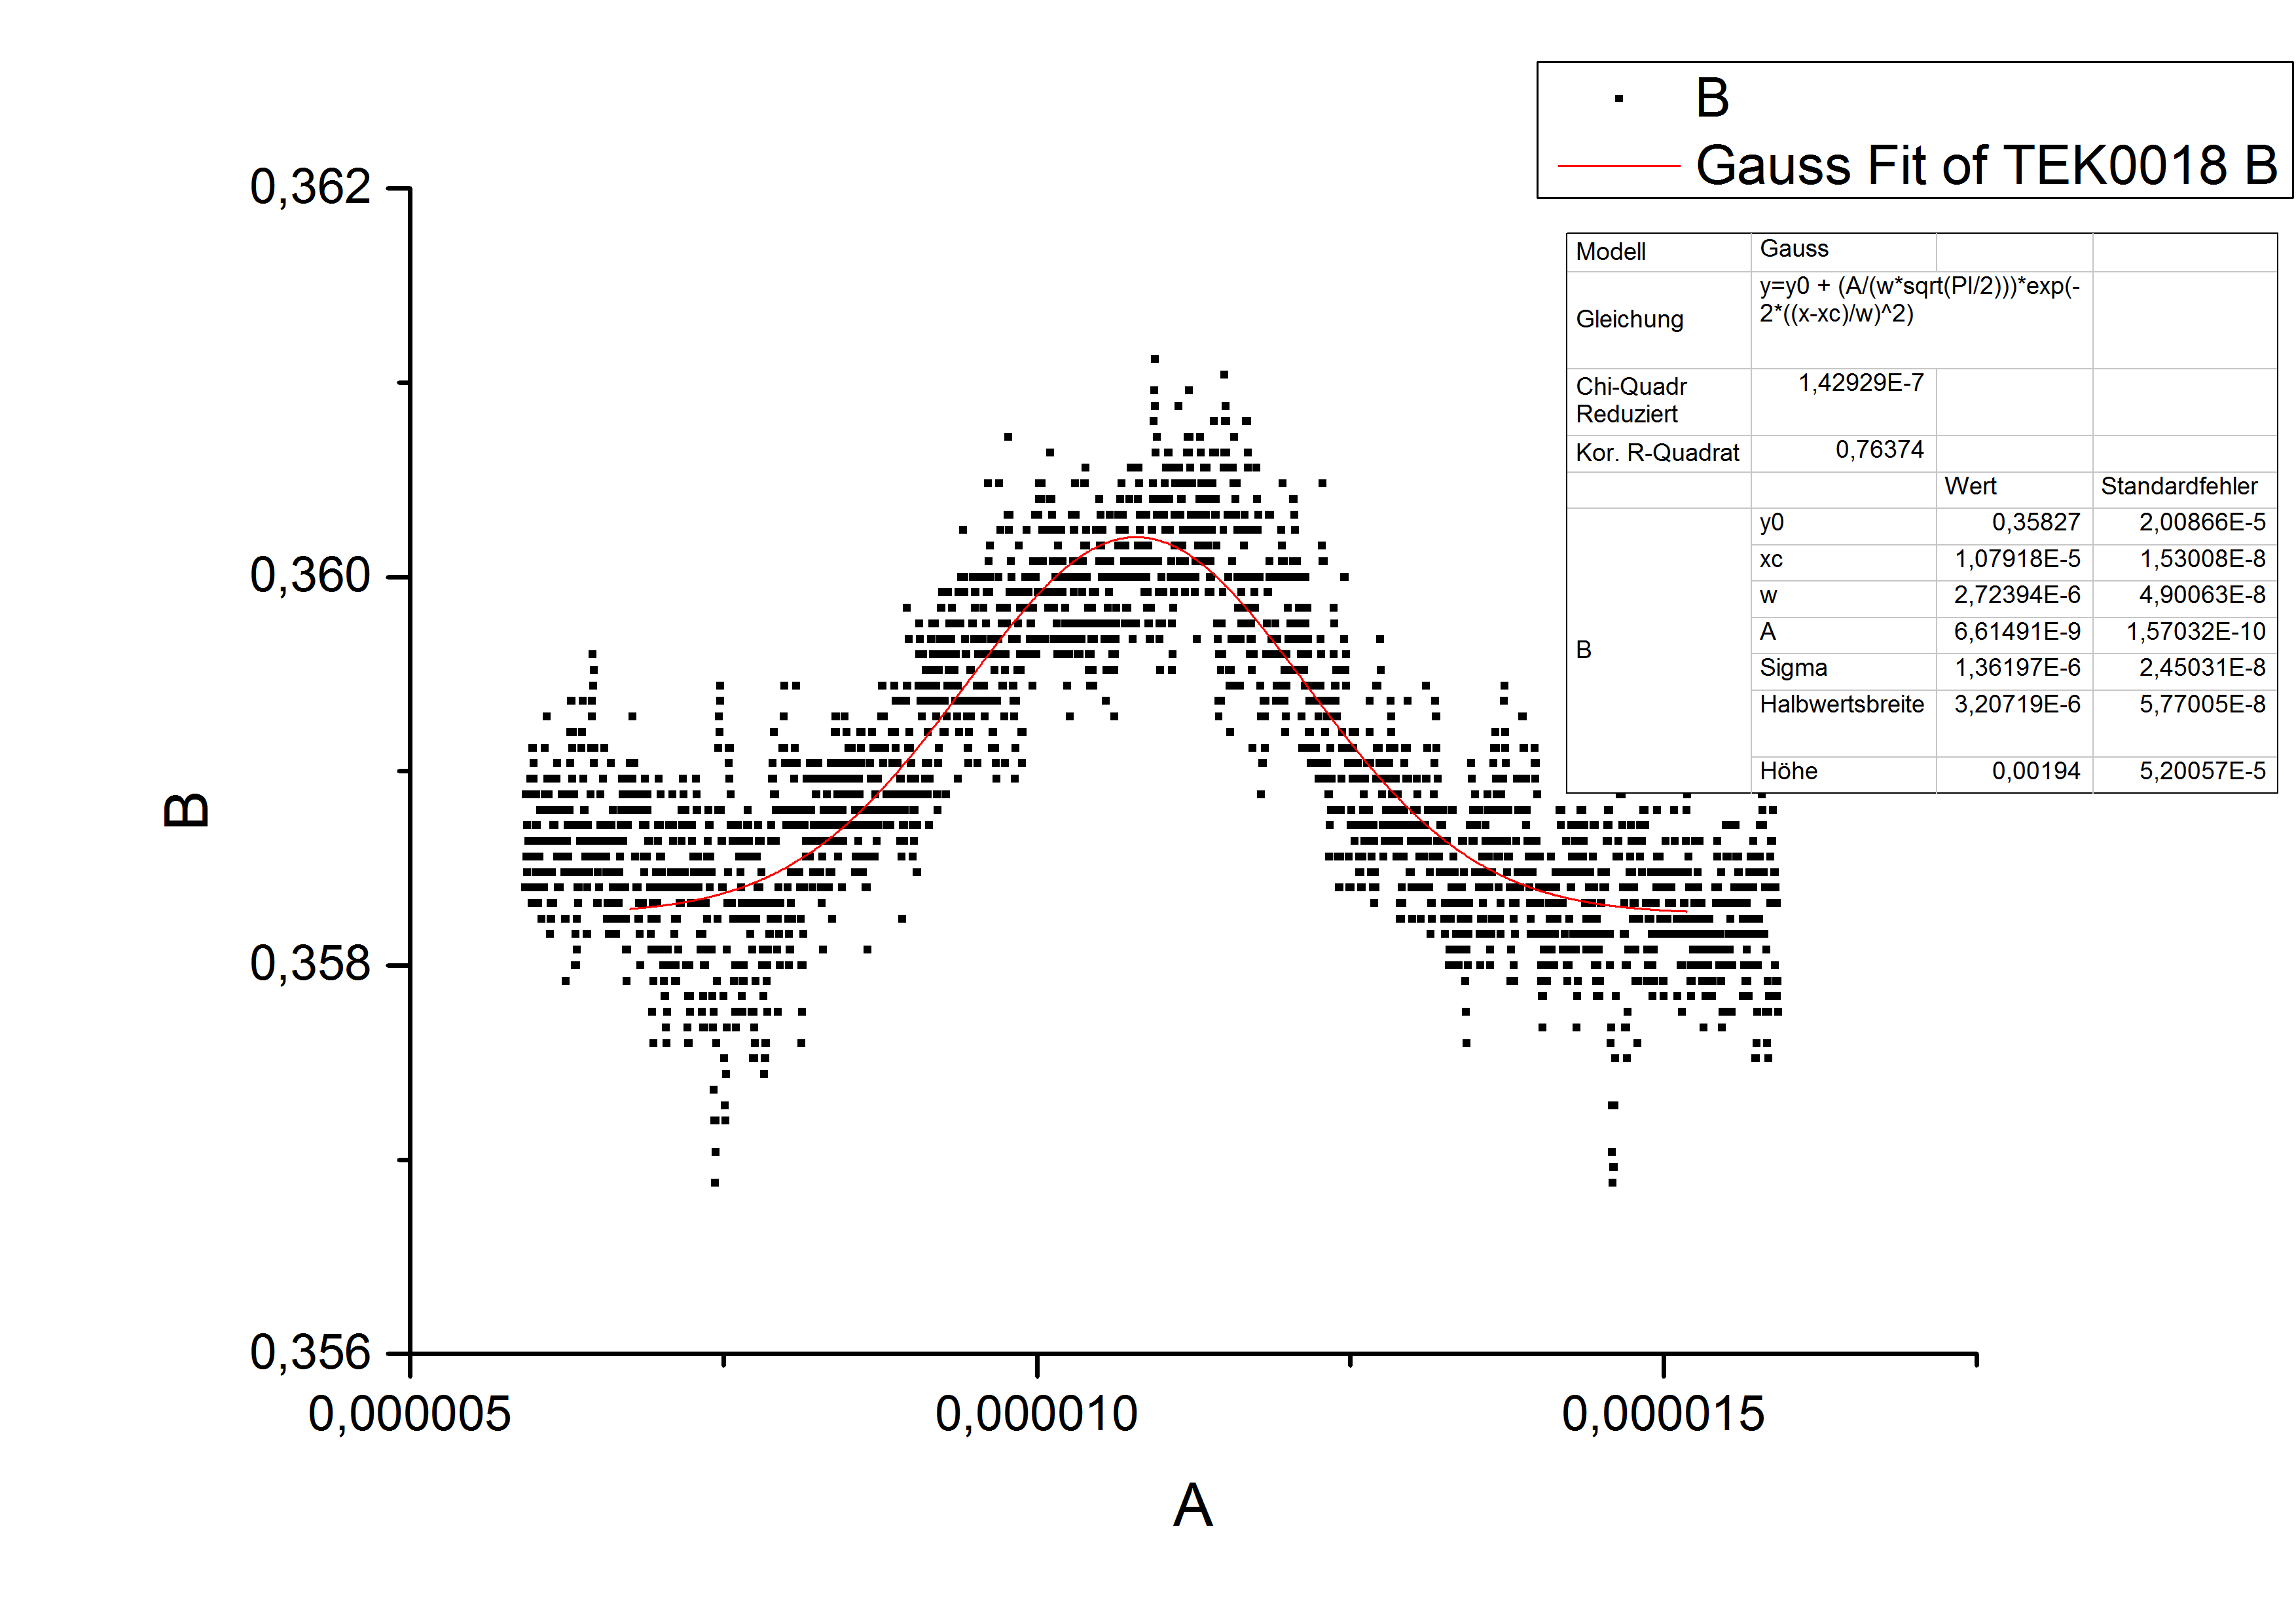
\includegraphics[scale=0.25]{Bilder/Teil2/22}
\caption{Graph at 46V.}
\label{fig:22}
\end{center}
\end{figure}
\begin{figure}[h]
\begin{center}
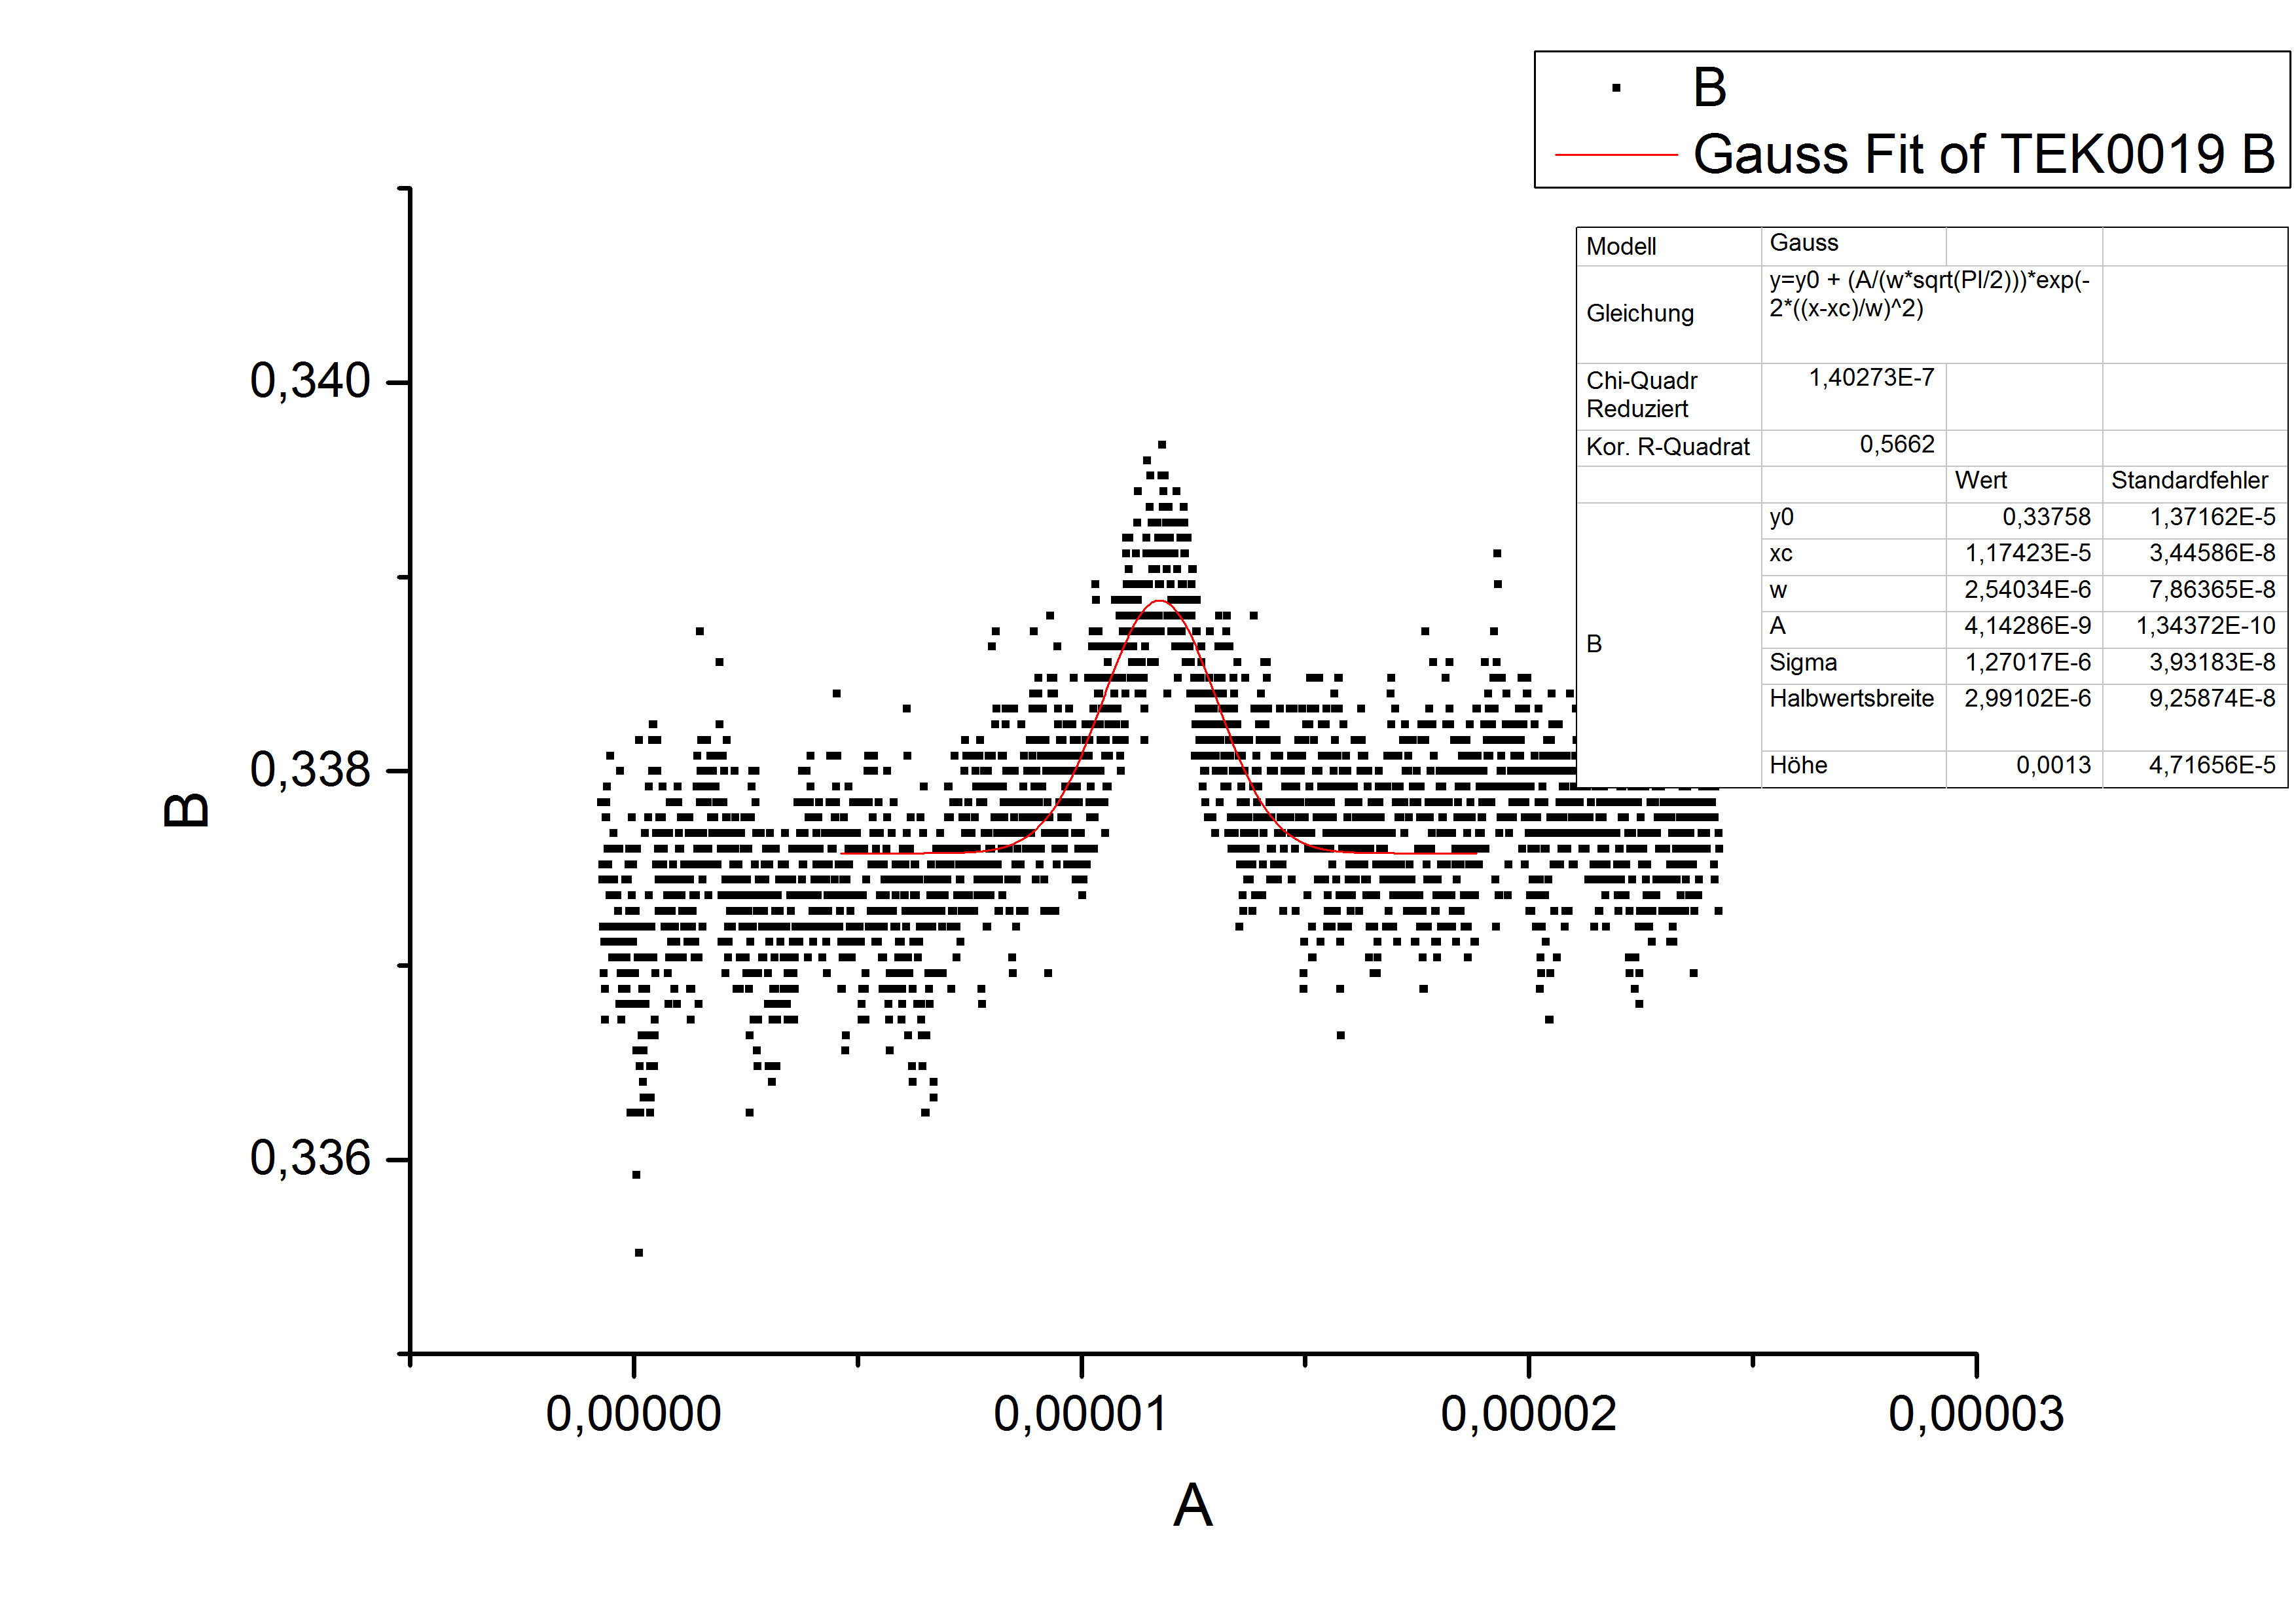
\includegraphics[scale=0.25]{Bilder/Teil2/23}
\caption{Graph at 42V.}
\label{fig:23}
\end{center}
\end{figure}
\begin{figure}[h]
\begin{center}
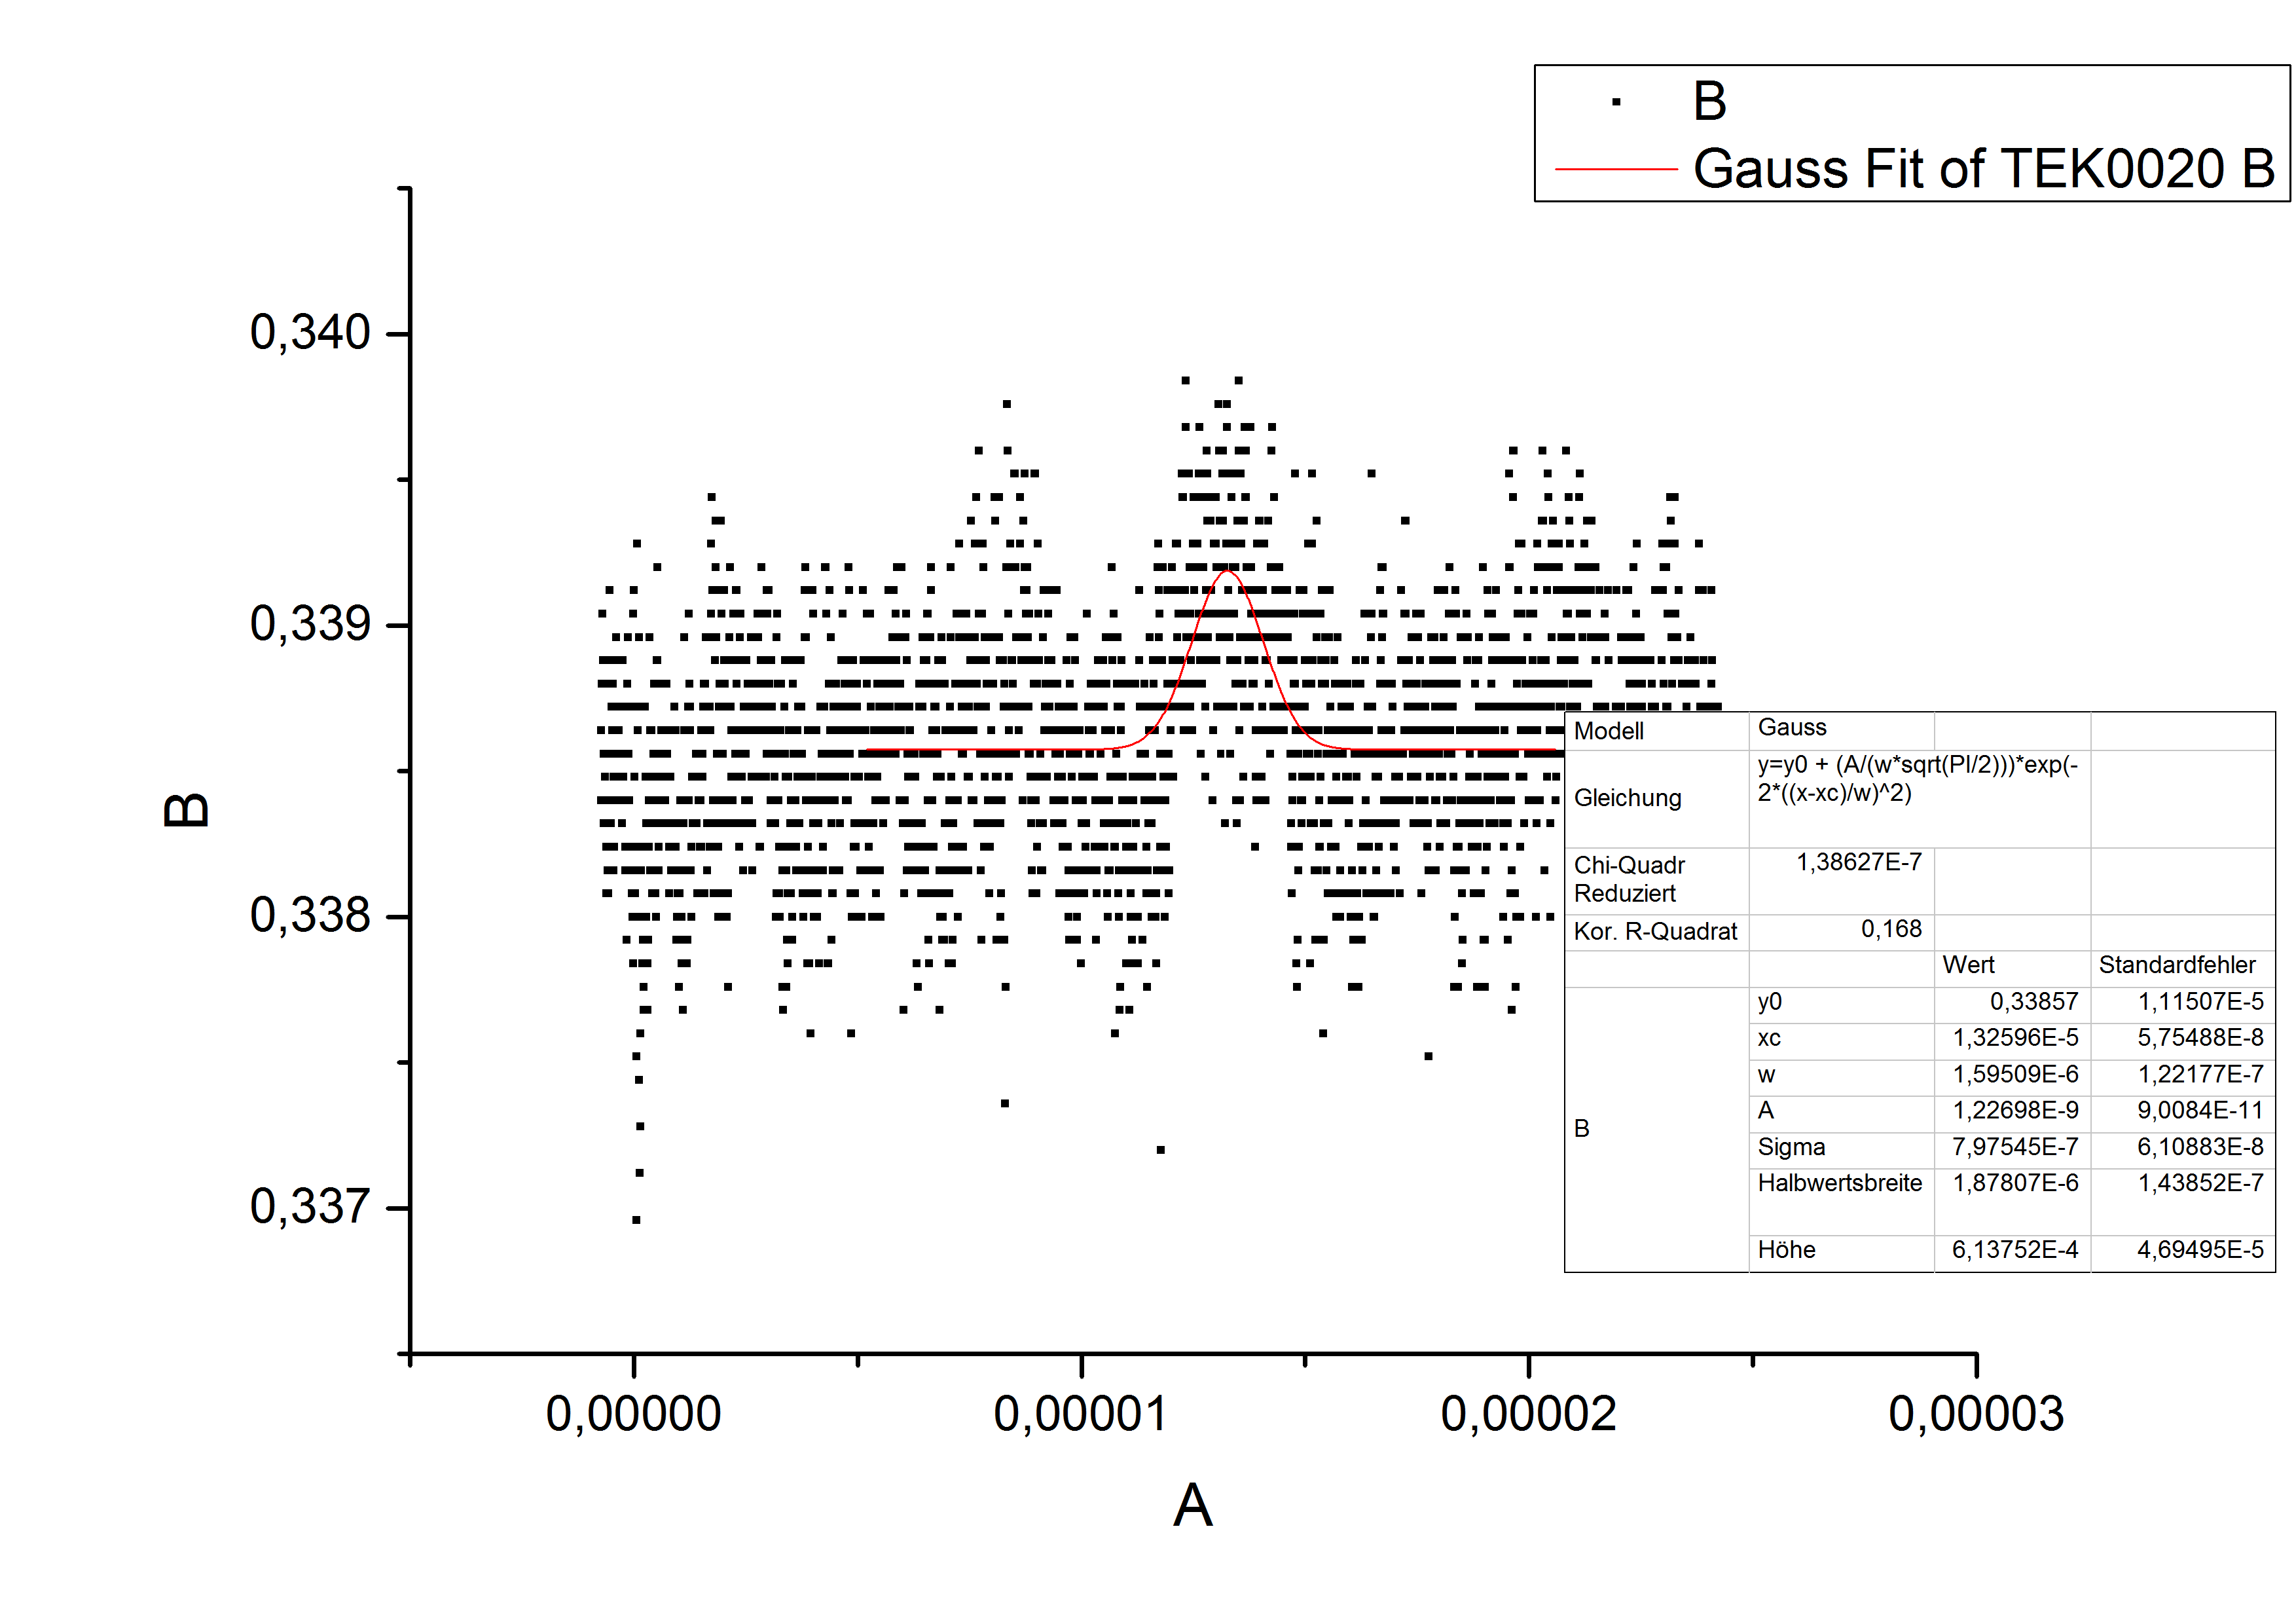
\includegraphics[scale=0.25]{Bilder/Teil2/24}
\caption{Graph 36V.}
\label{fig:24}
\end{center}
\end{figure}
\begin{figure}[h]
\begin{center}
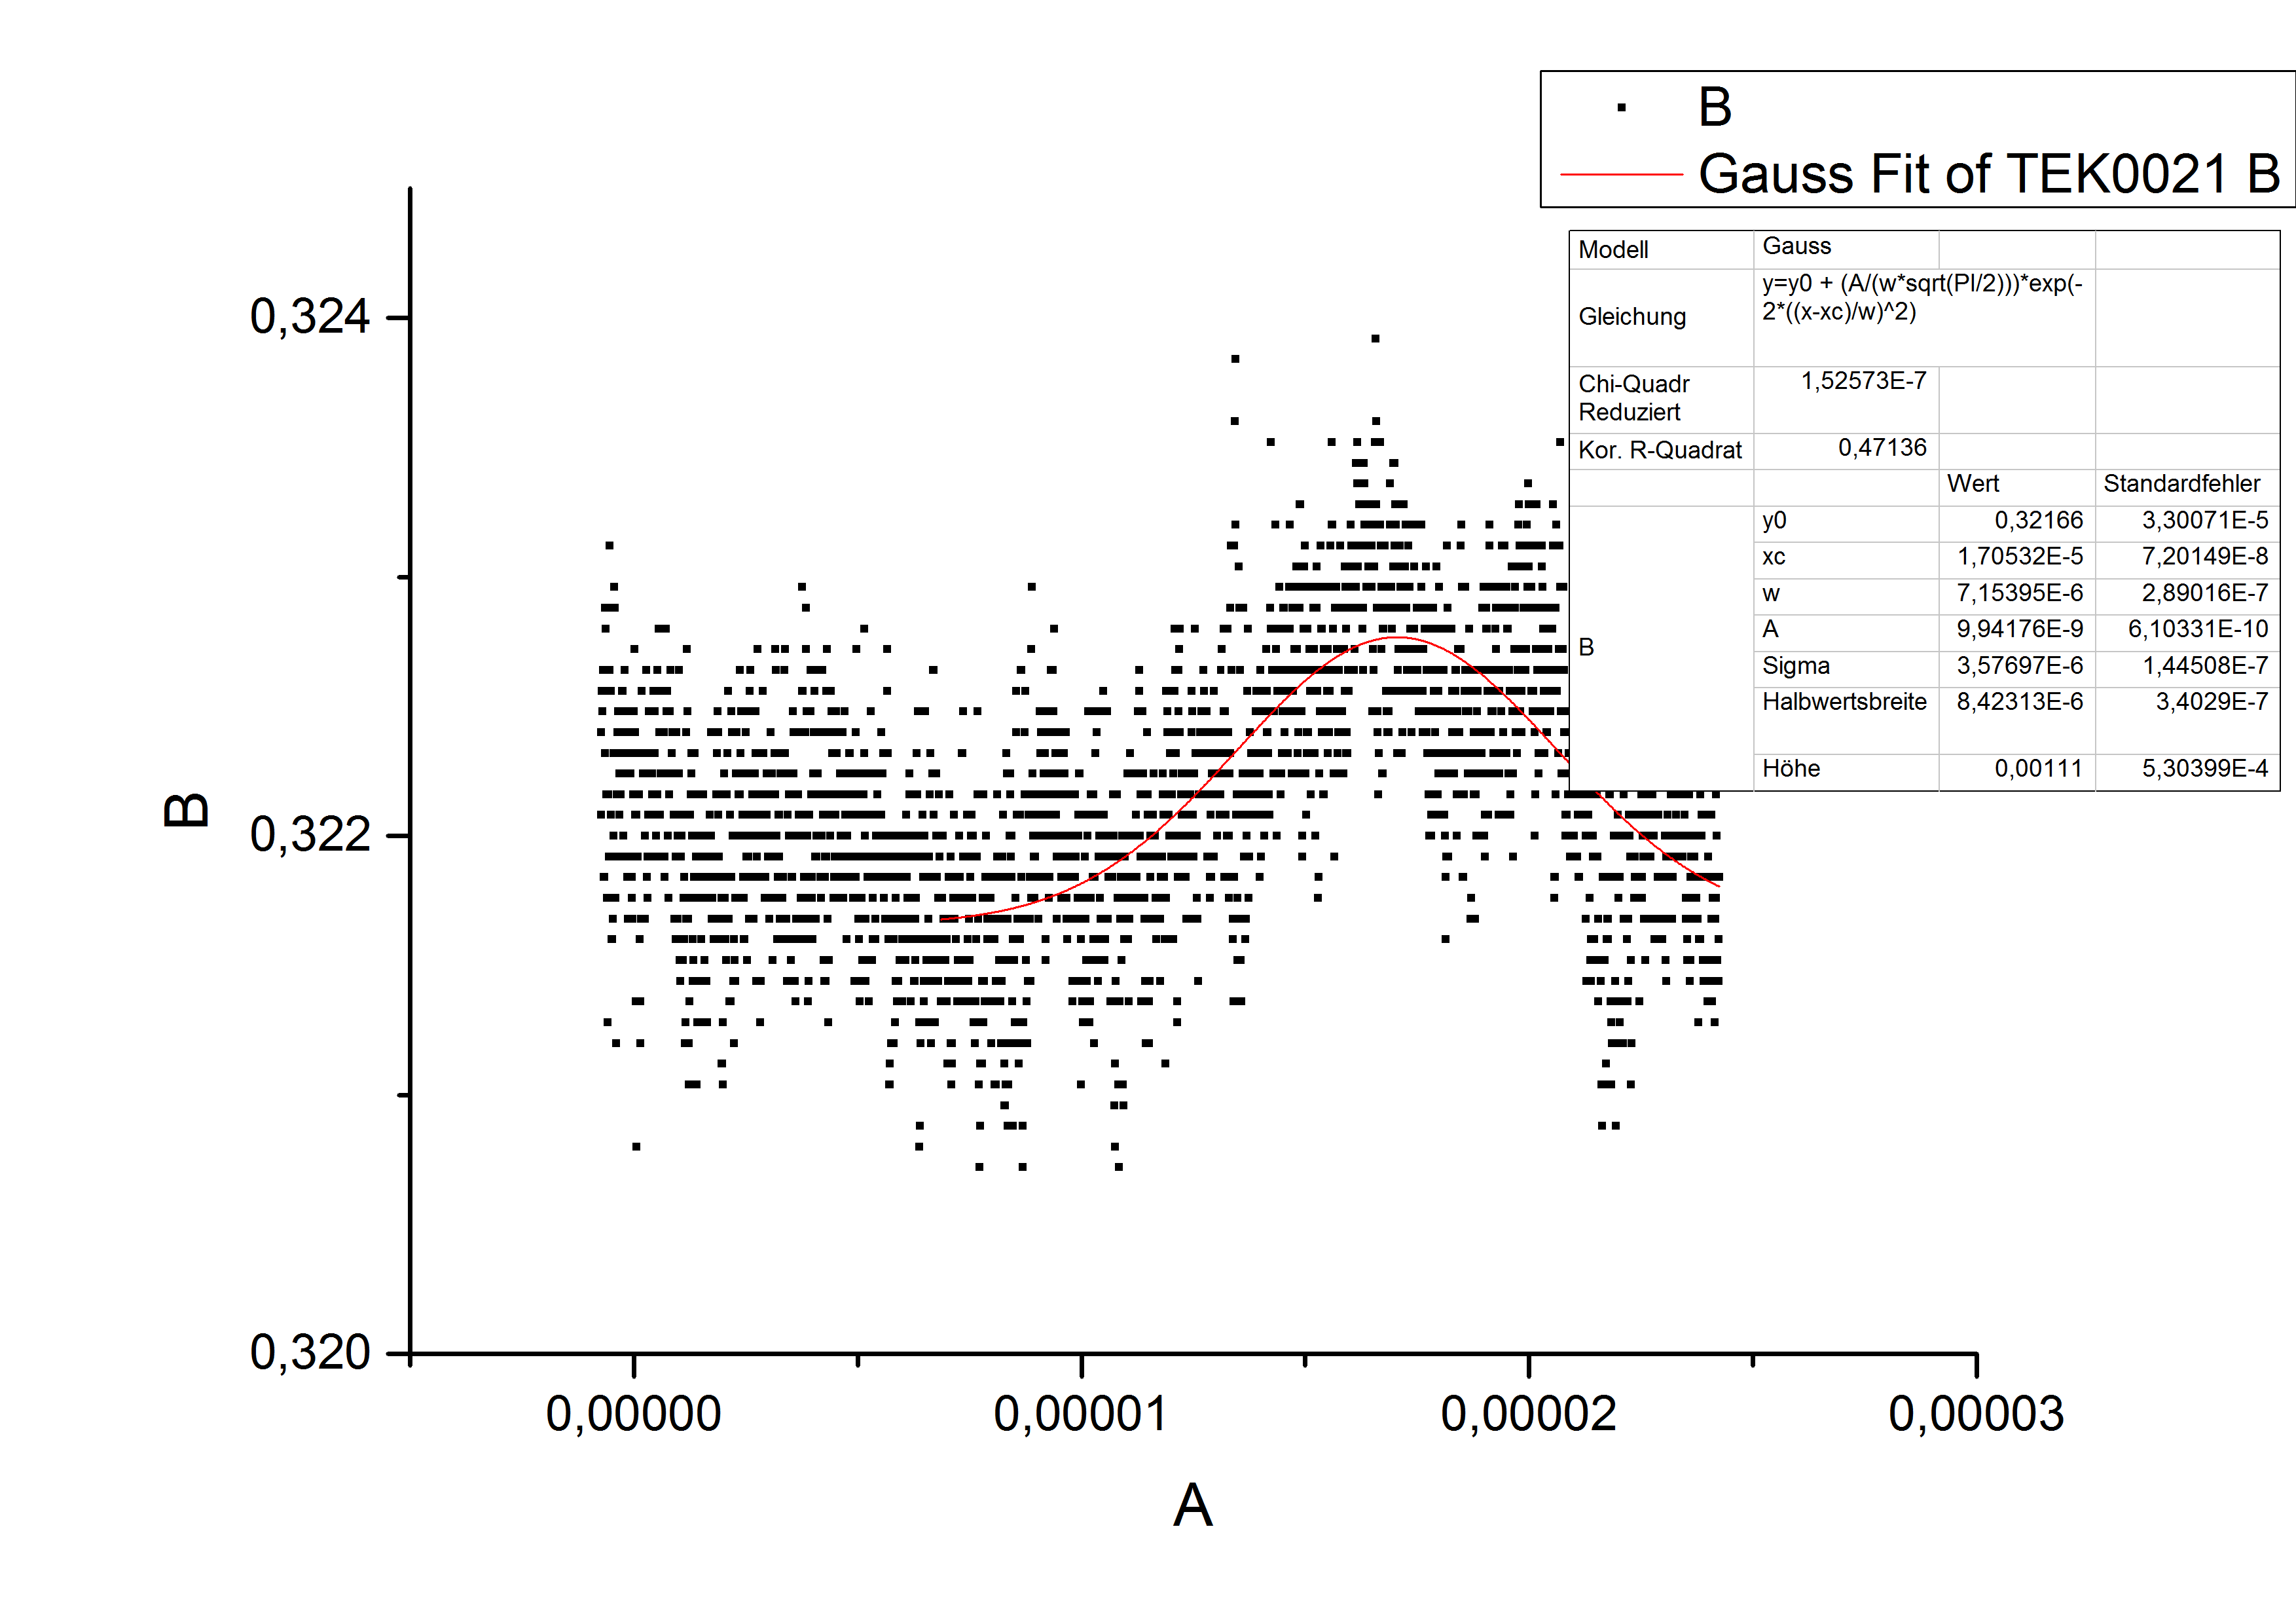
\includegraphics[scale=0.25]{Bilder/Teil2/25}
\caption{Graph 32V.}
\label{fig:25}
\end{center}
\end{figure}
\begin{figure}[h]
\begin{center}
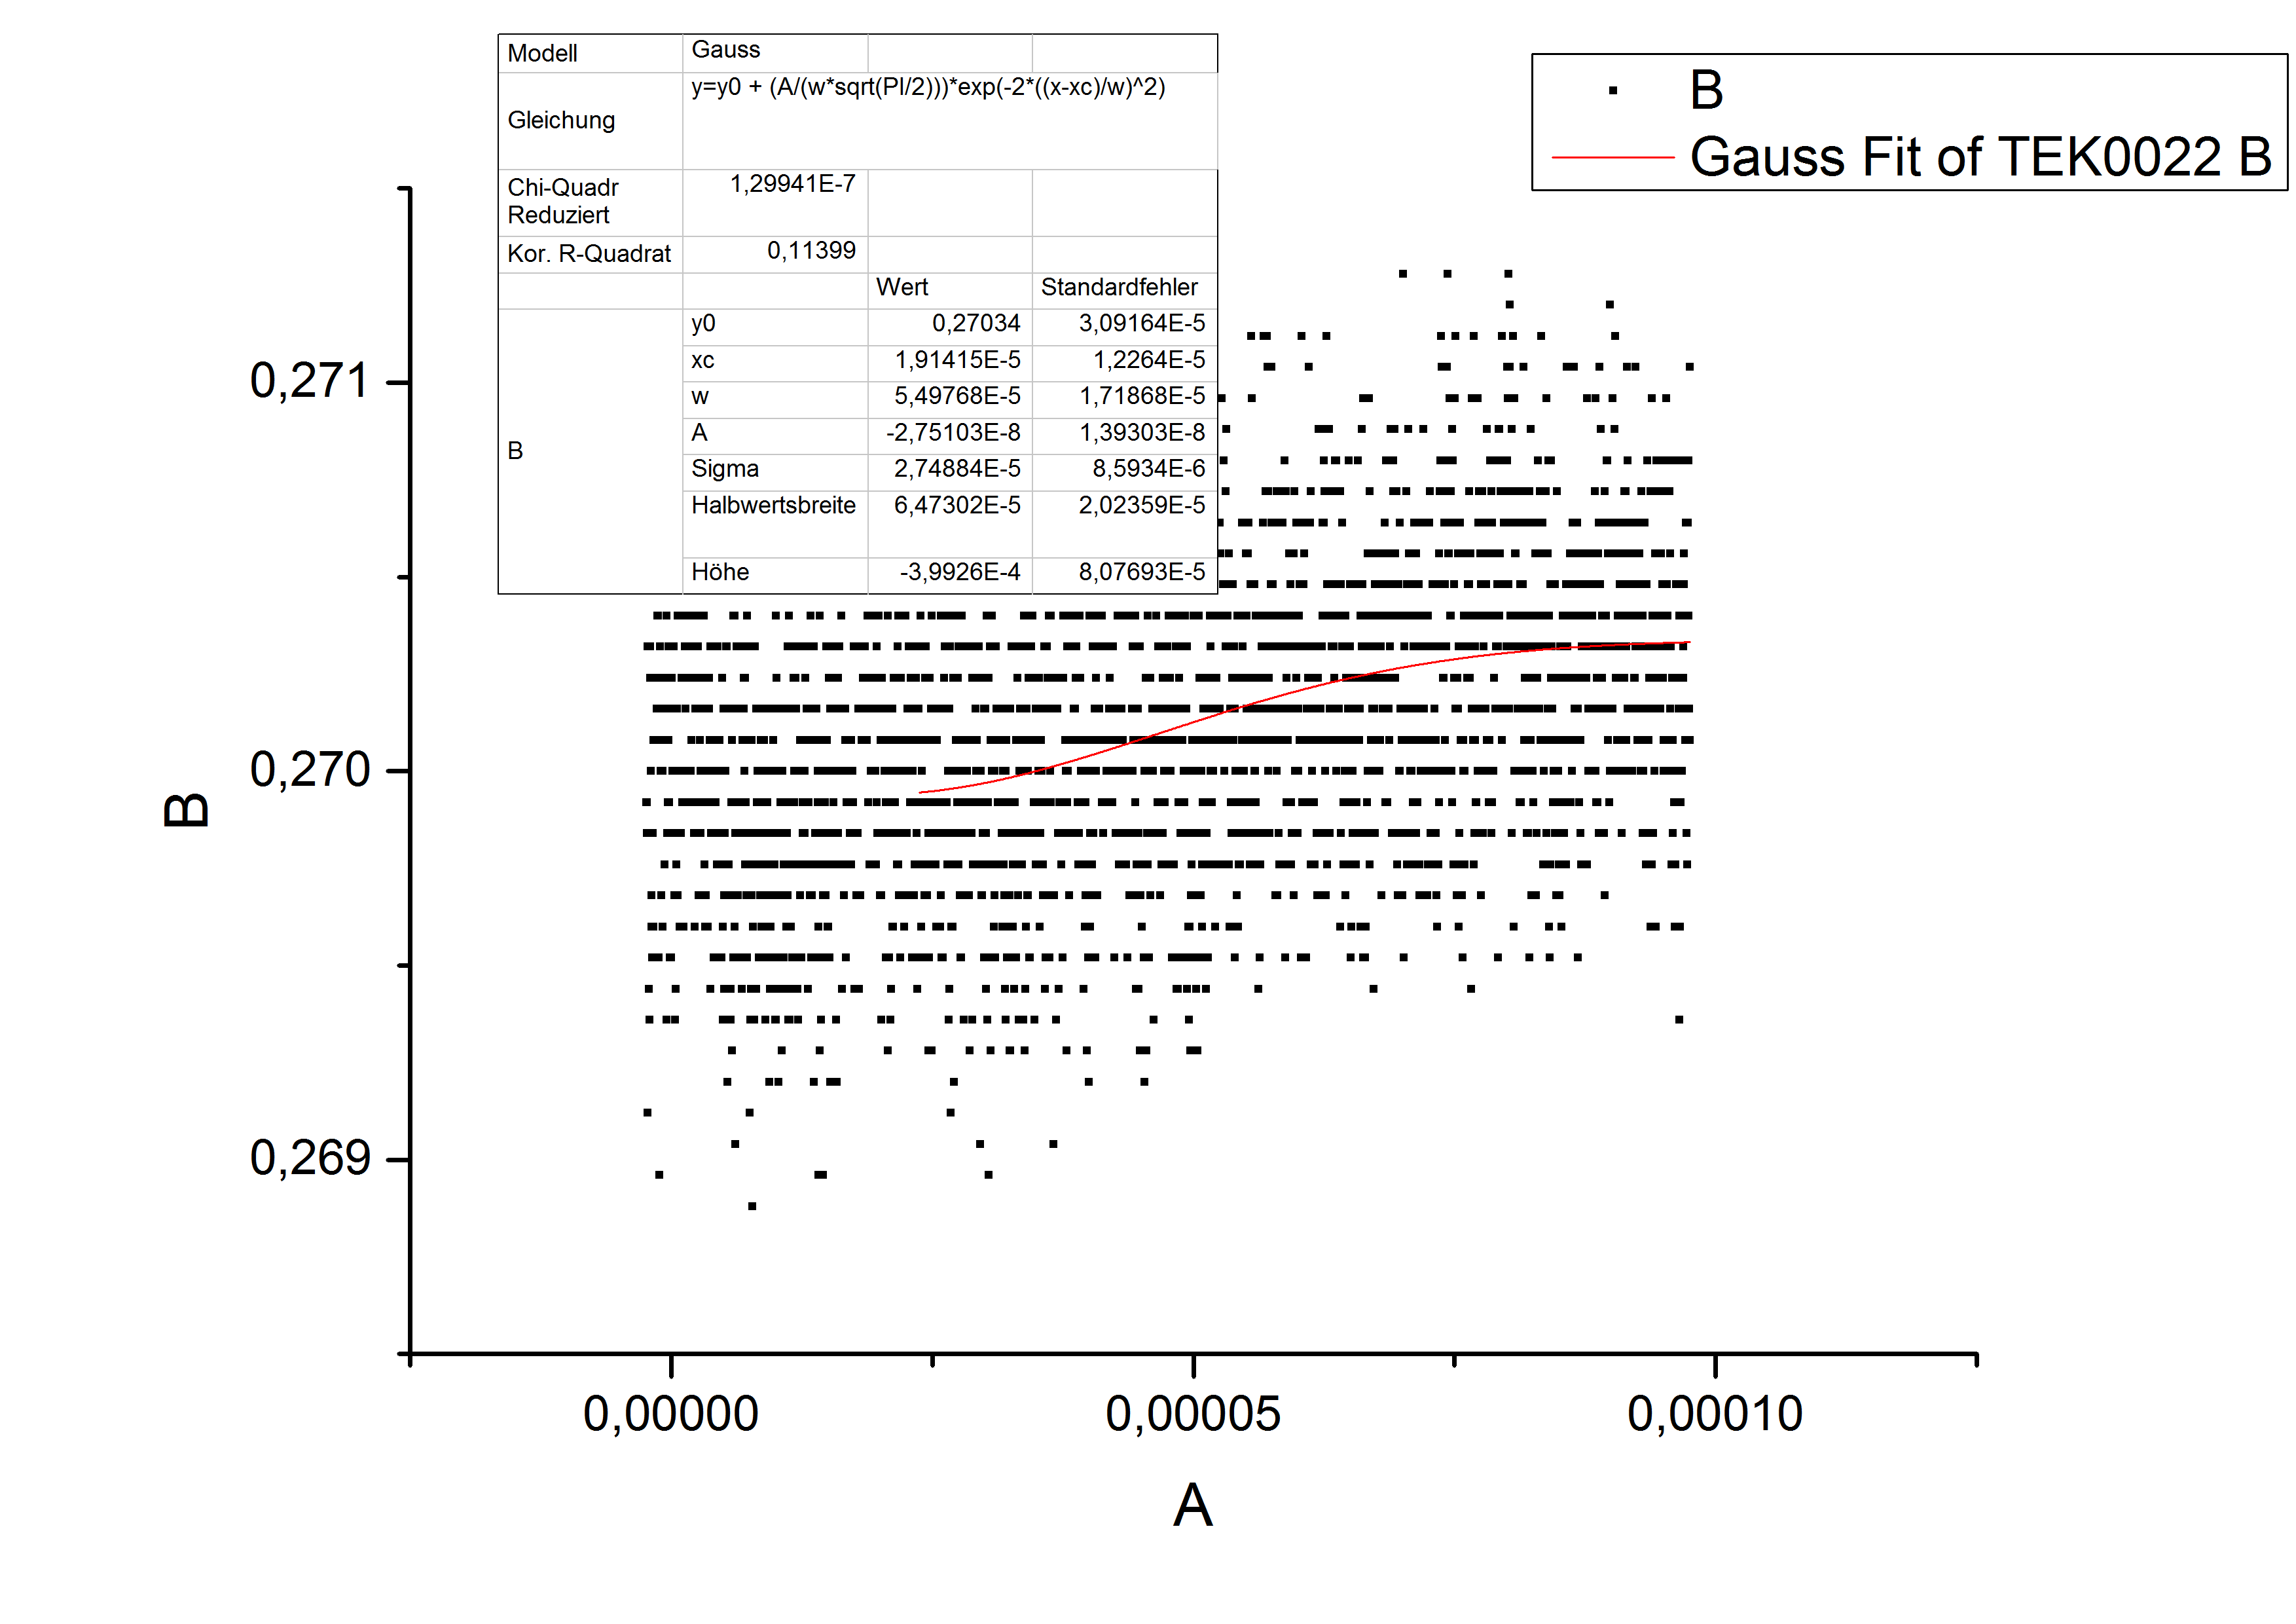
\includegraphics[scale=0.25]{Bilder/Teil2/26}
\caption{Graph 28V.}
\label{fig:26}
\end{center}
\end{figure}
\clearpage
\section*{Experiment No.3}
\begin{figure}[h]
\begin{center}
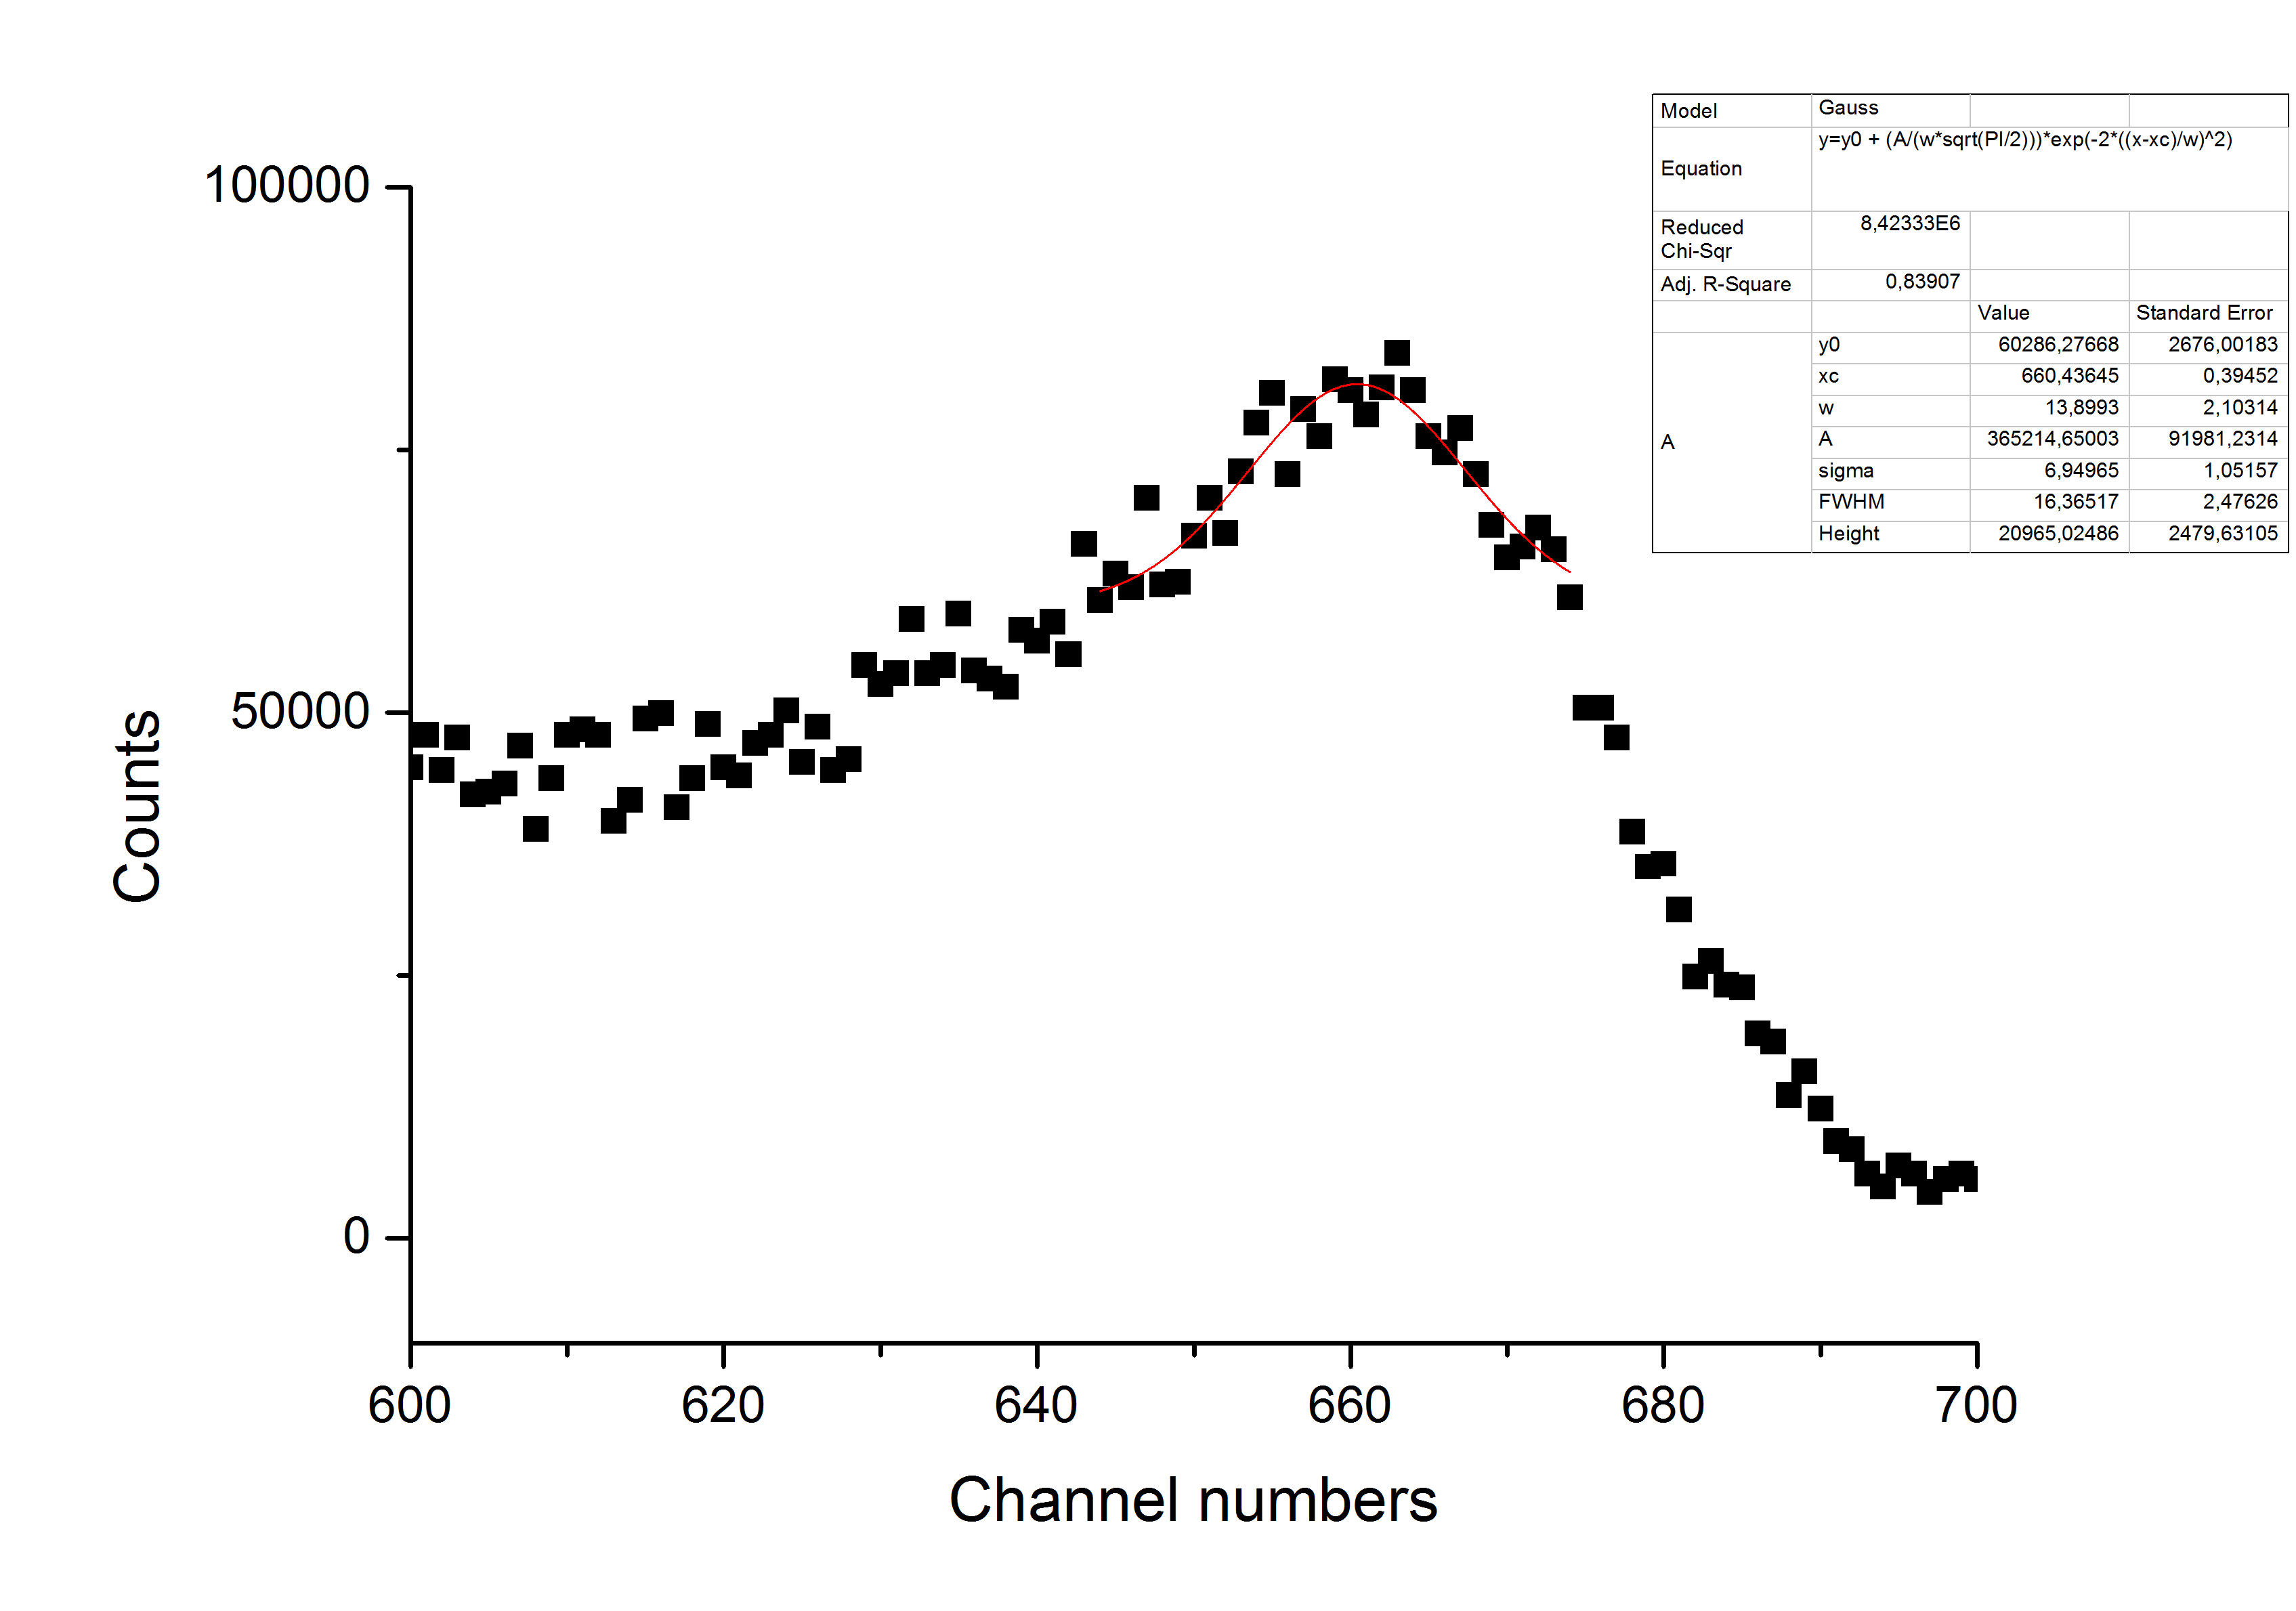
\includegraphics[scale=0.15]{Bilder/Teil3/122keV_CdTe_korrekt}
\caption{122keV, CdTe, with correction of the peak}
\label{fig:CdTeK}
\end{center}
\end{figure}
\begin{figure}[h]
\begin{center}
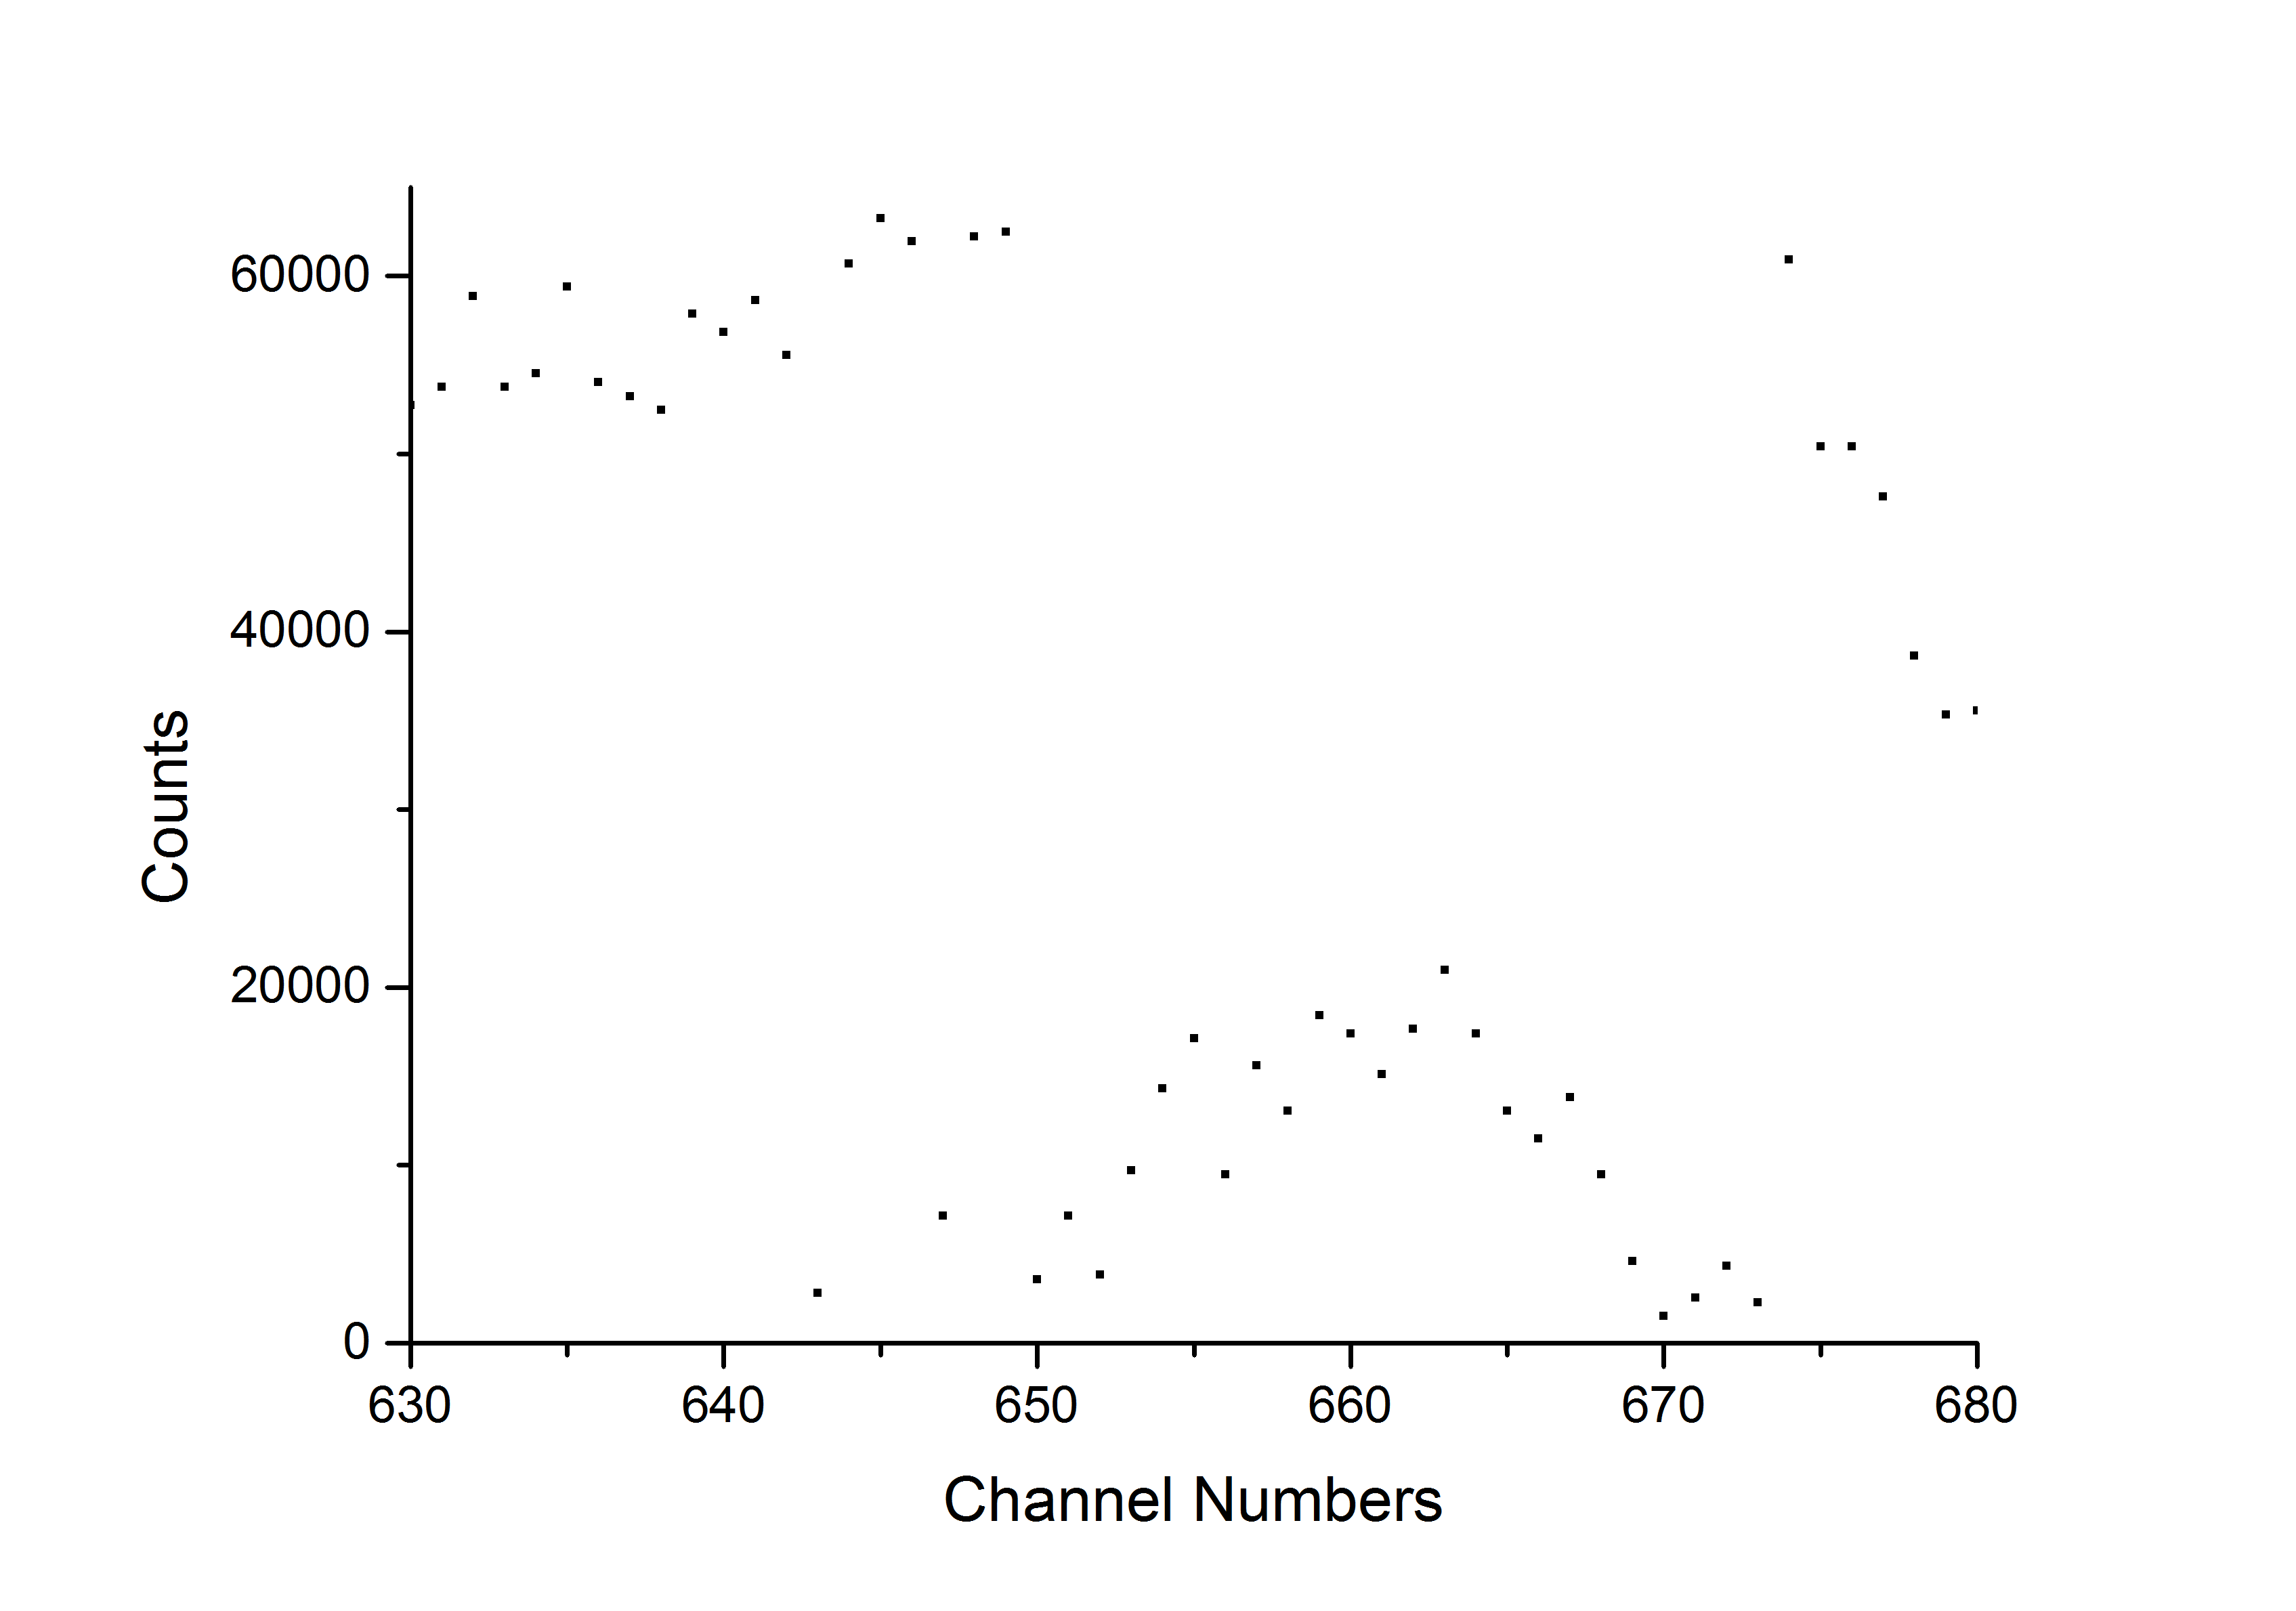
\includegraphics[scale=0.15]{Bilder/Teil3/122keV_CdTe_ohne}
\caption{122keV, CdTe, without correction of the peak}
\label{fig:CdTeO}
\end{center}
\end{figure}
\begin{figure}[h]
\begin{center}
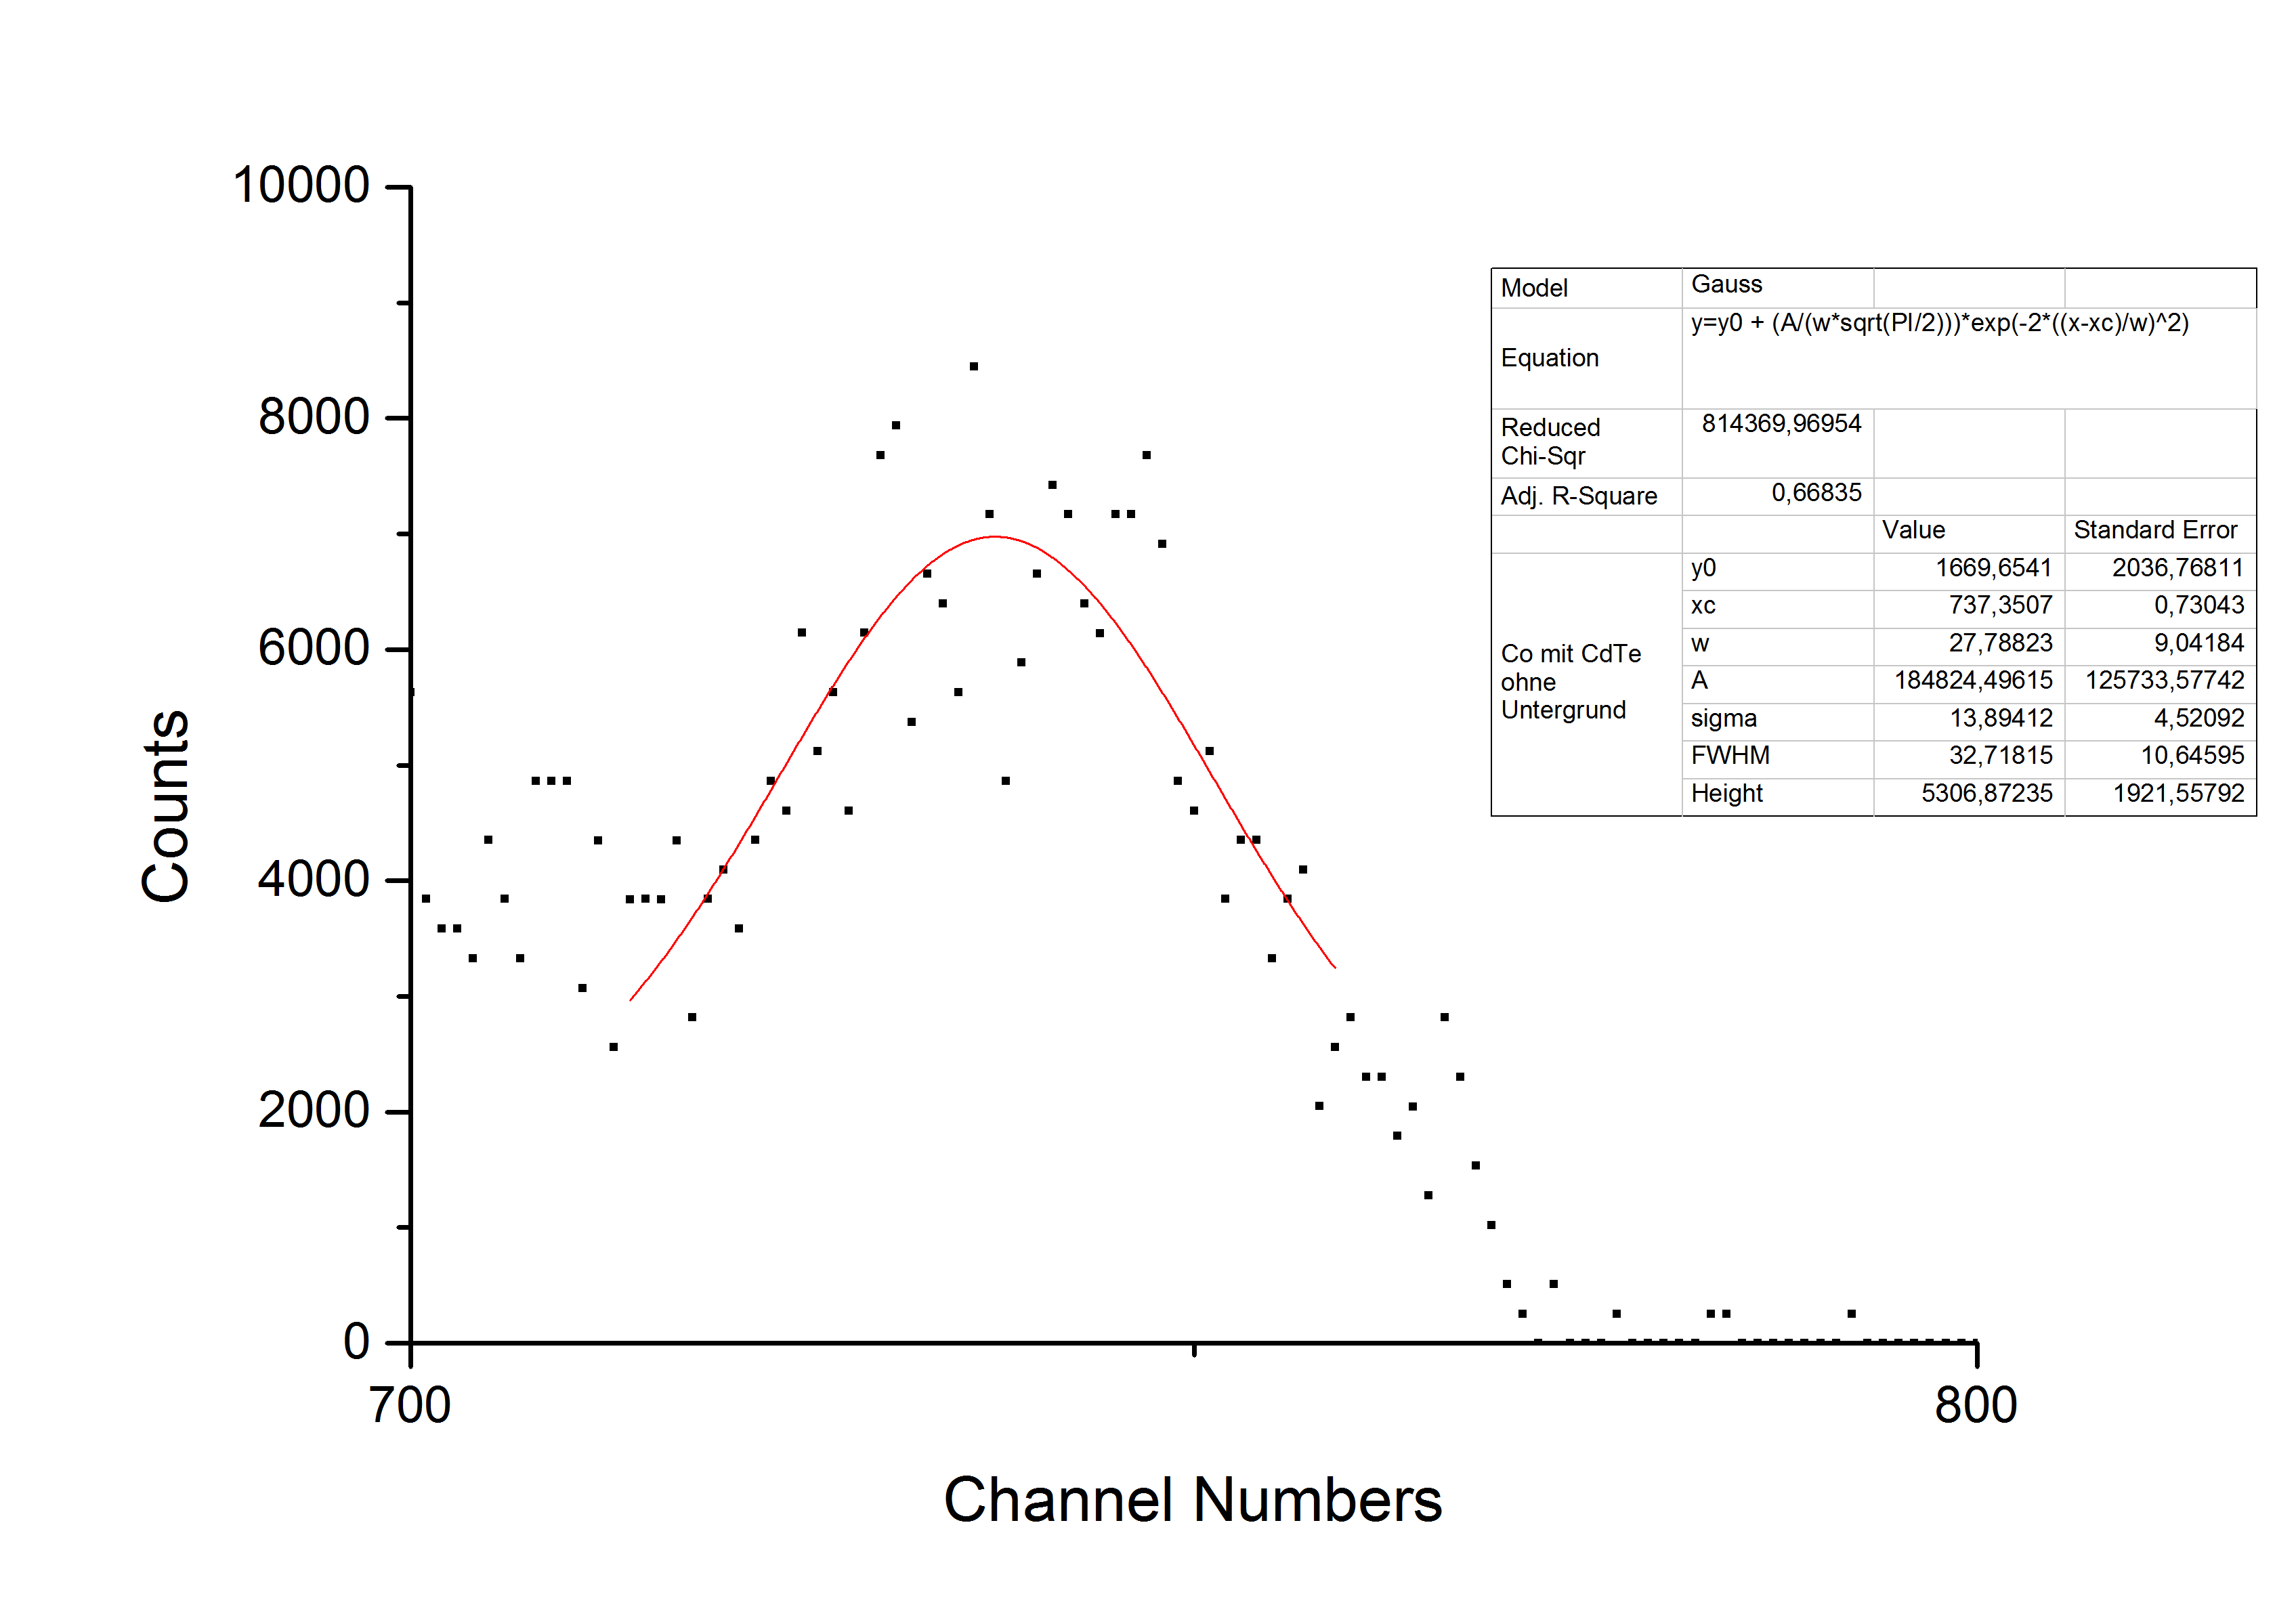
\includegraphics[scale=0.15]{Bilder/Teil3/136keV_CdTe}
\caption{136keV peak, CdTe}
\label{fig:CdTe}
\end{center}
\end{figure}
\begin{figure}[h]
\begin{center}
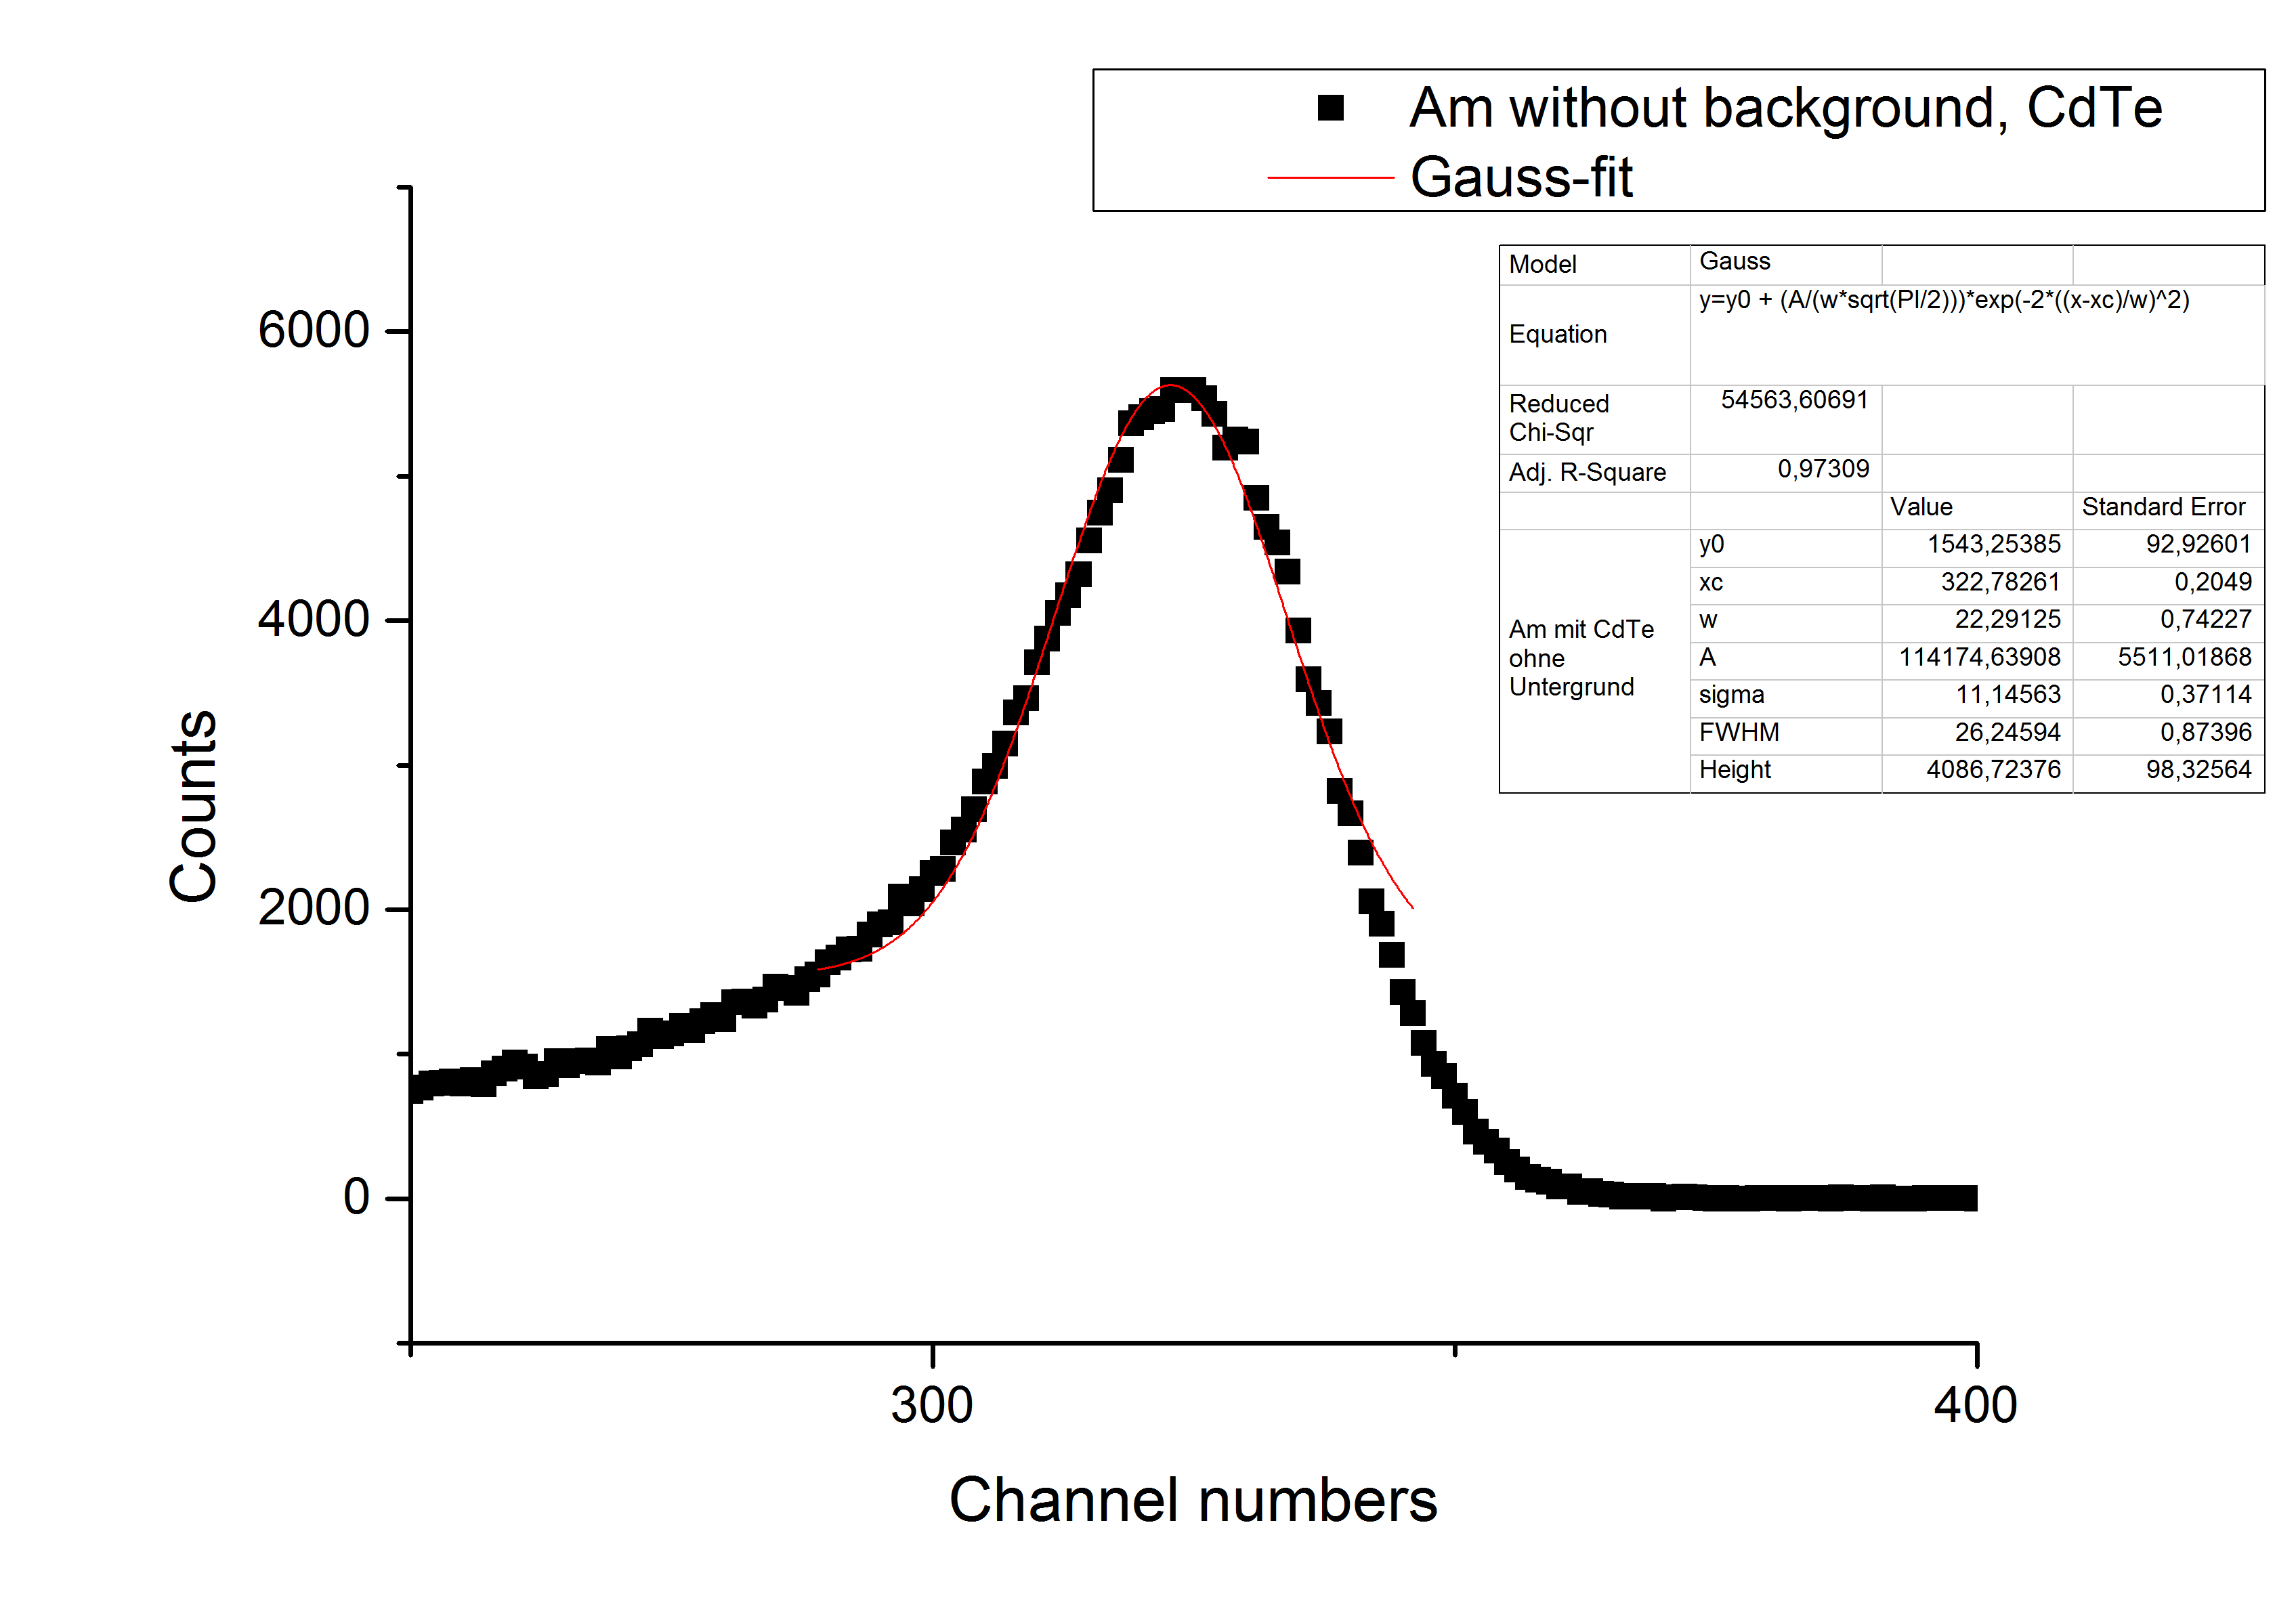
\includegraphics[scale=0.15]{Bilder/Teil3/Am_Cd}
\caption{Am with CdTe-detector}
\label{fig:AmCdTe}
\end{center}
\end{figure}
\begin{figure}[h]
\begin{center}
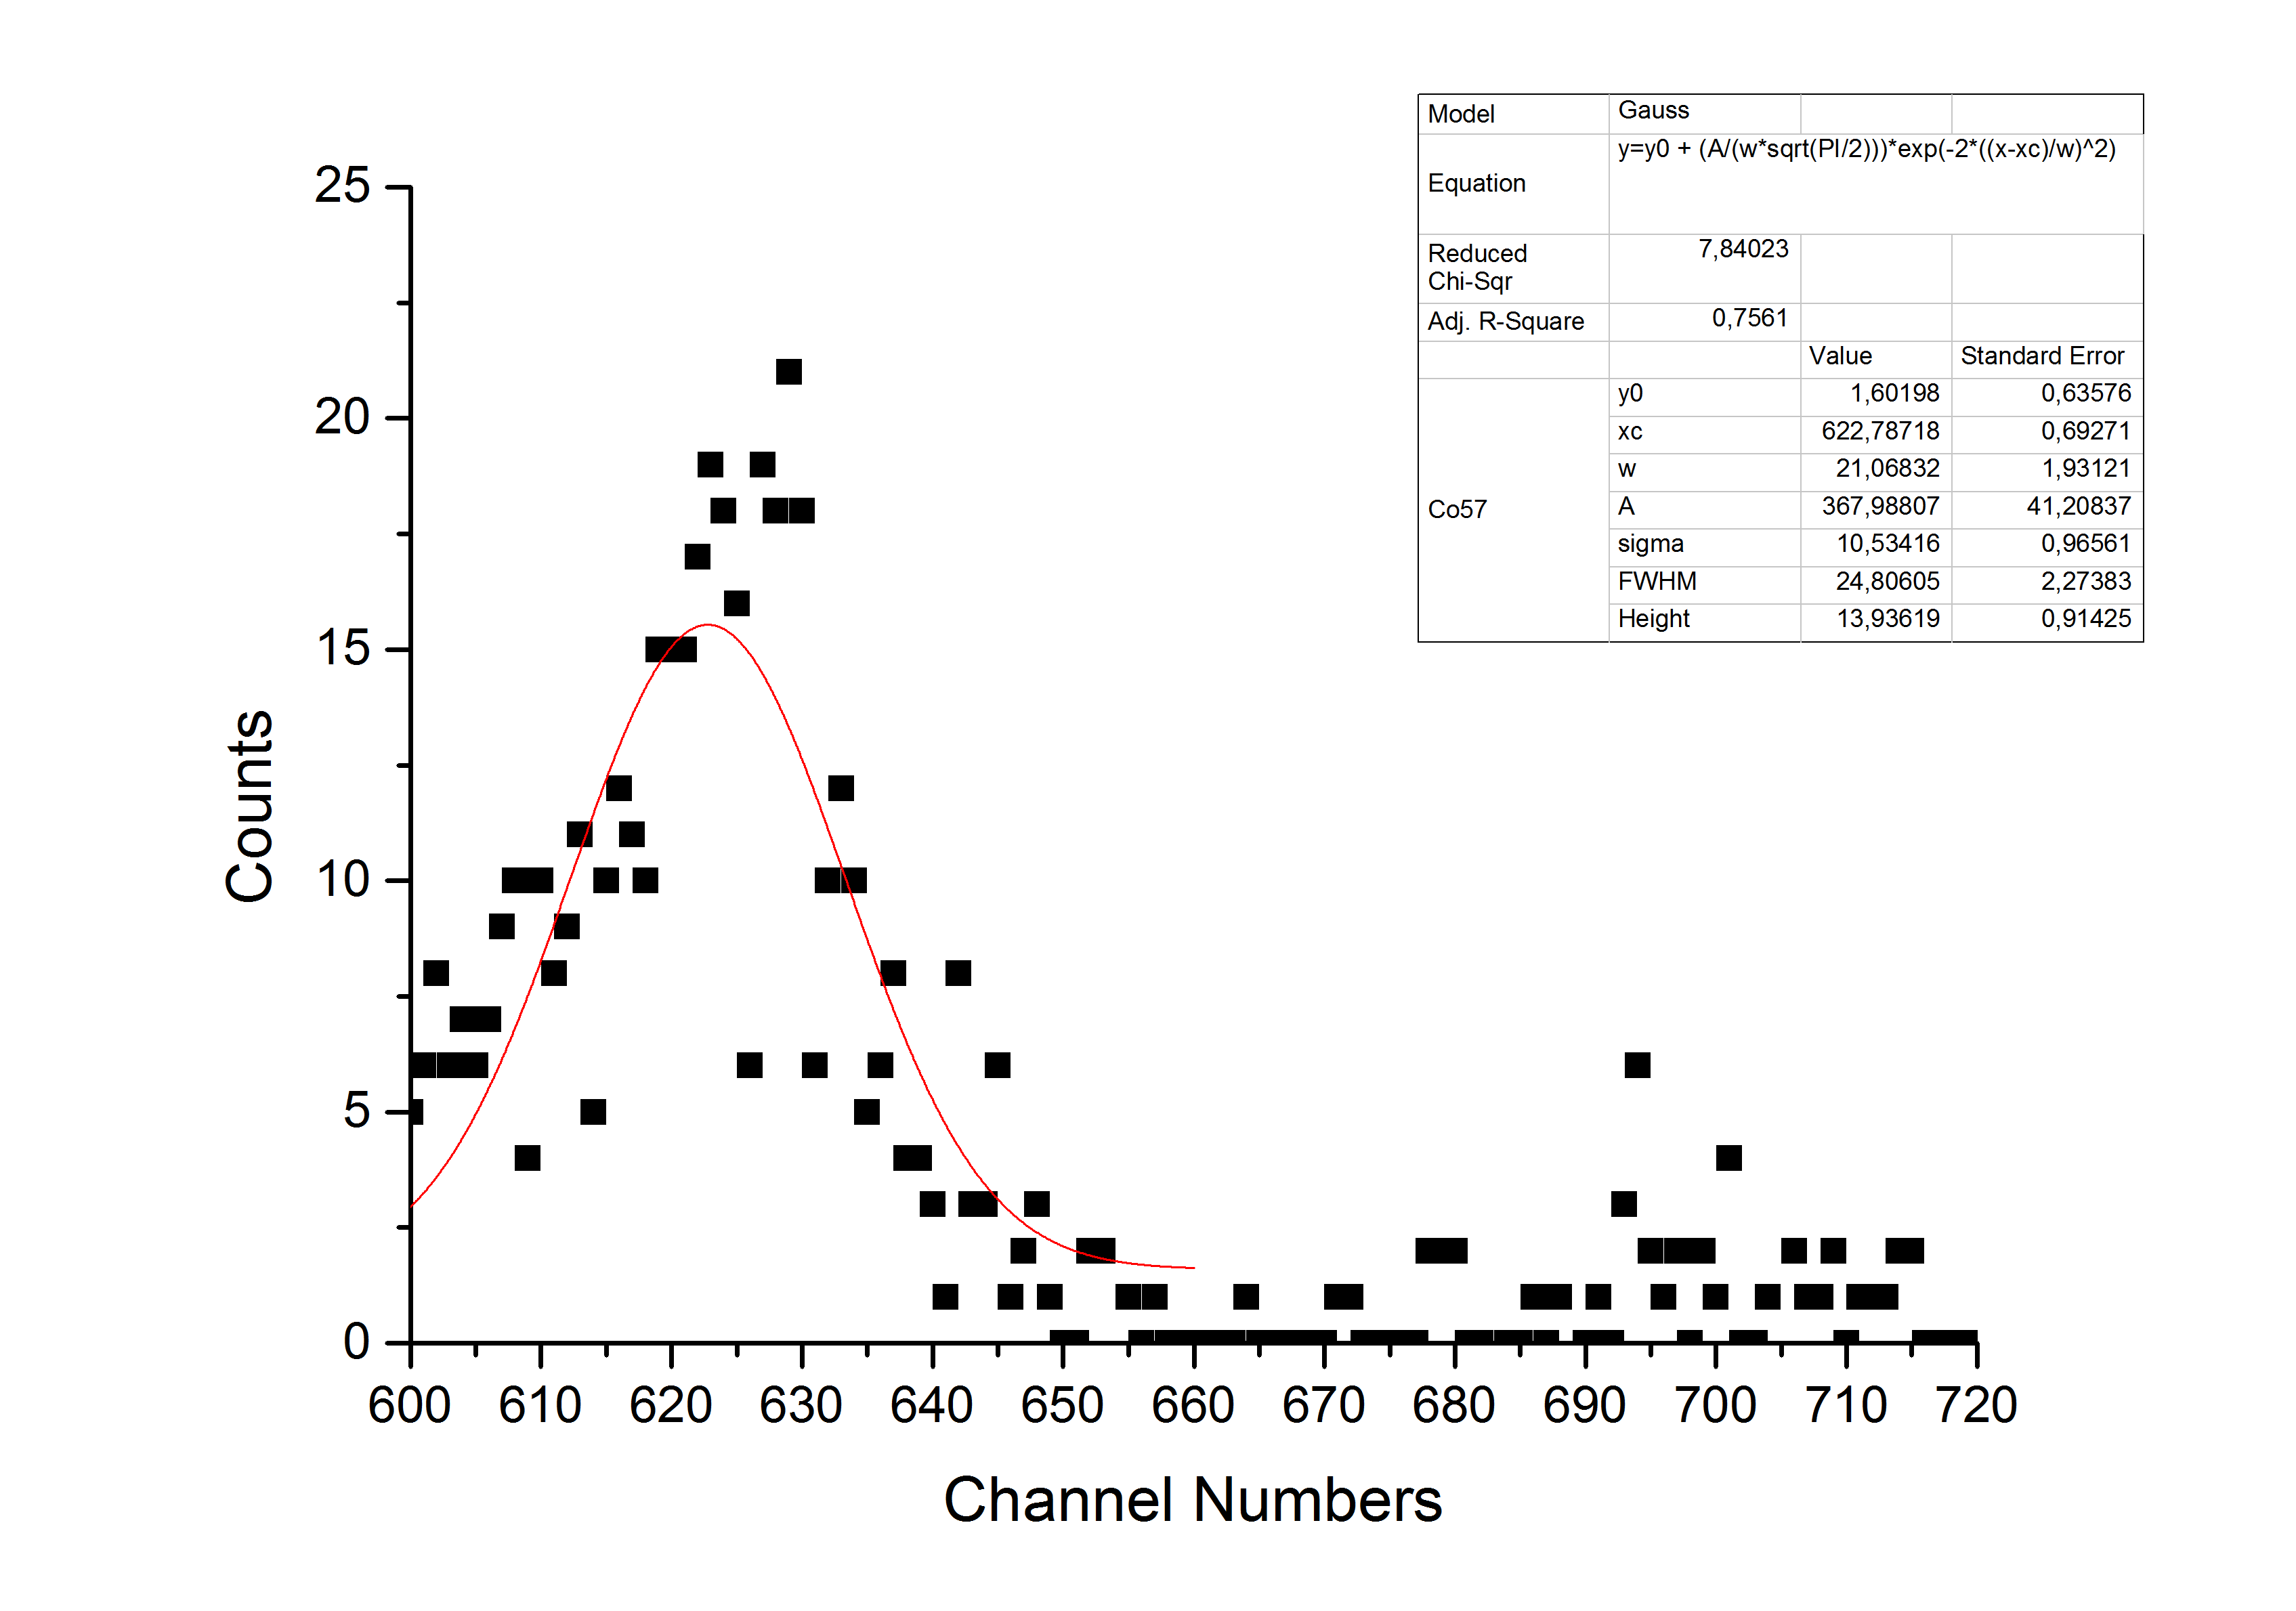
\includegraphics[scale=0.15]{Bilder/Teil3/122keV_Si}
\caption{122keV peak with Si-detector}
\label{fig:Si122}
\end{center}
\end{figure}
\begin{figure}[h]
\begin{center}
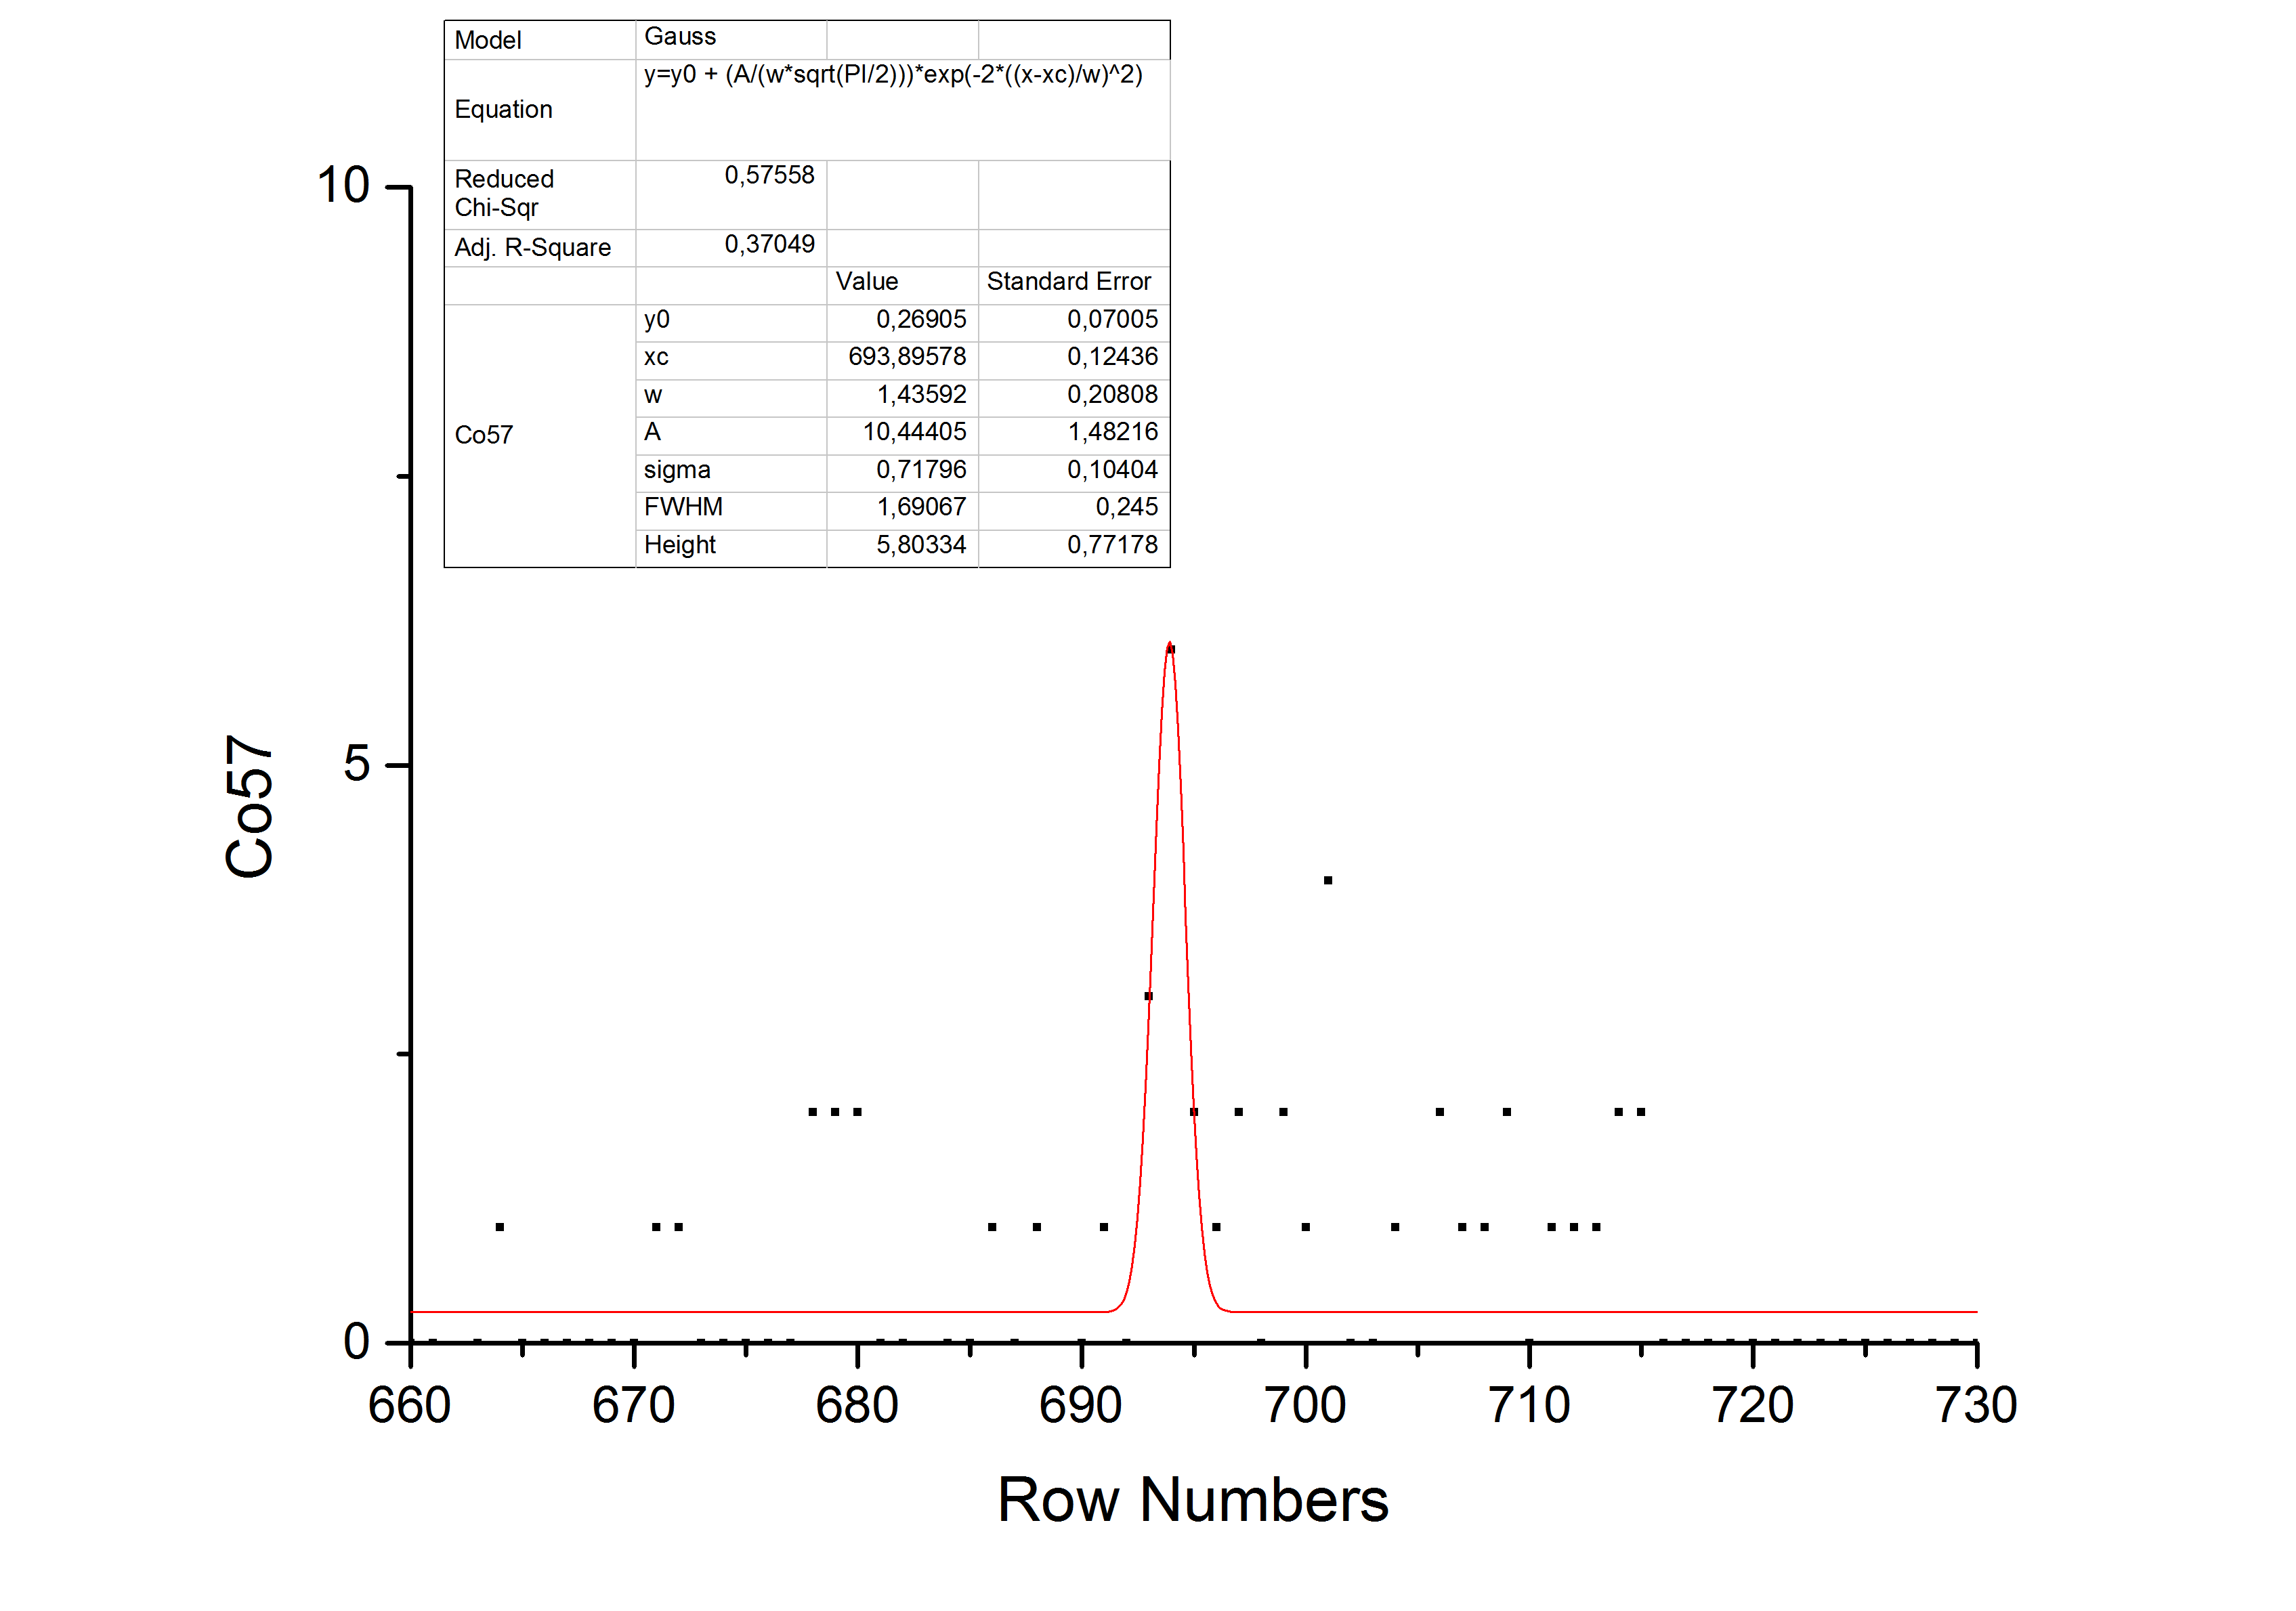
\includegraphics[scale=0.15]{Bilder/Teil3/136keV_Si}
\caption{136keV peak with Si-detector}
\label{fig:Si136}
\end{center}
\end{figure}
\begin{figure}[h]
\begin{center}
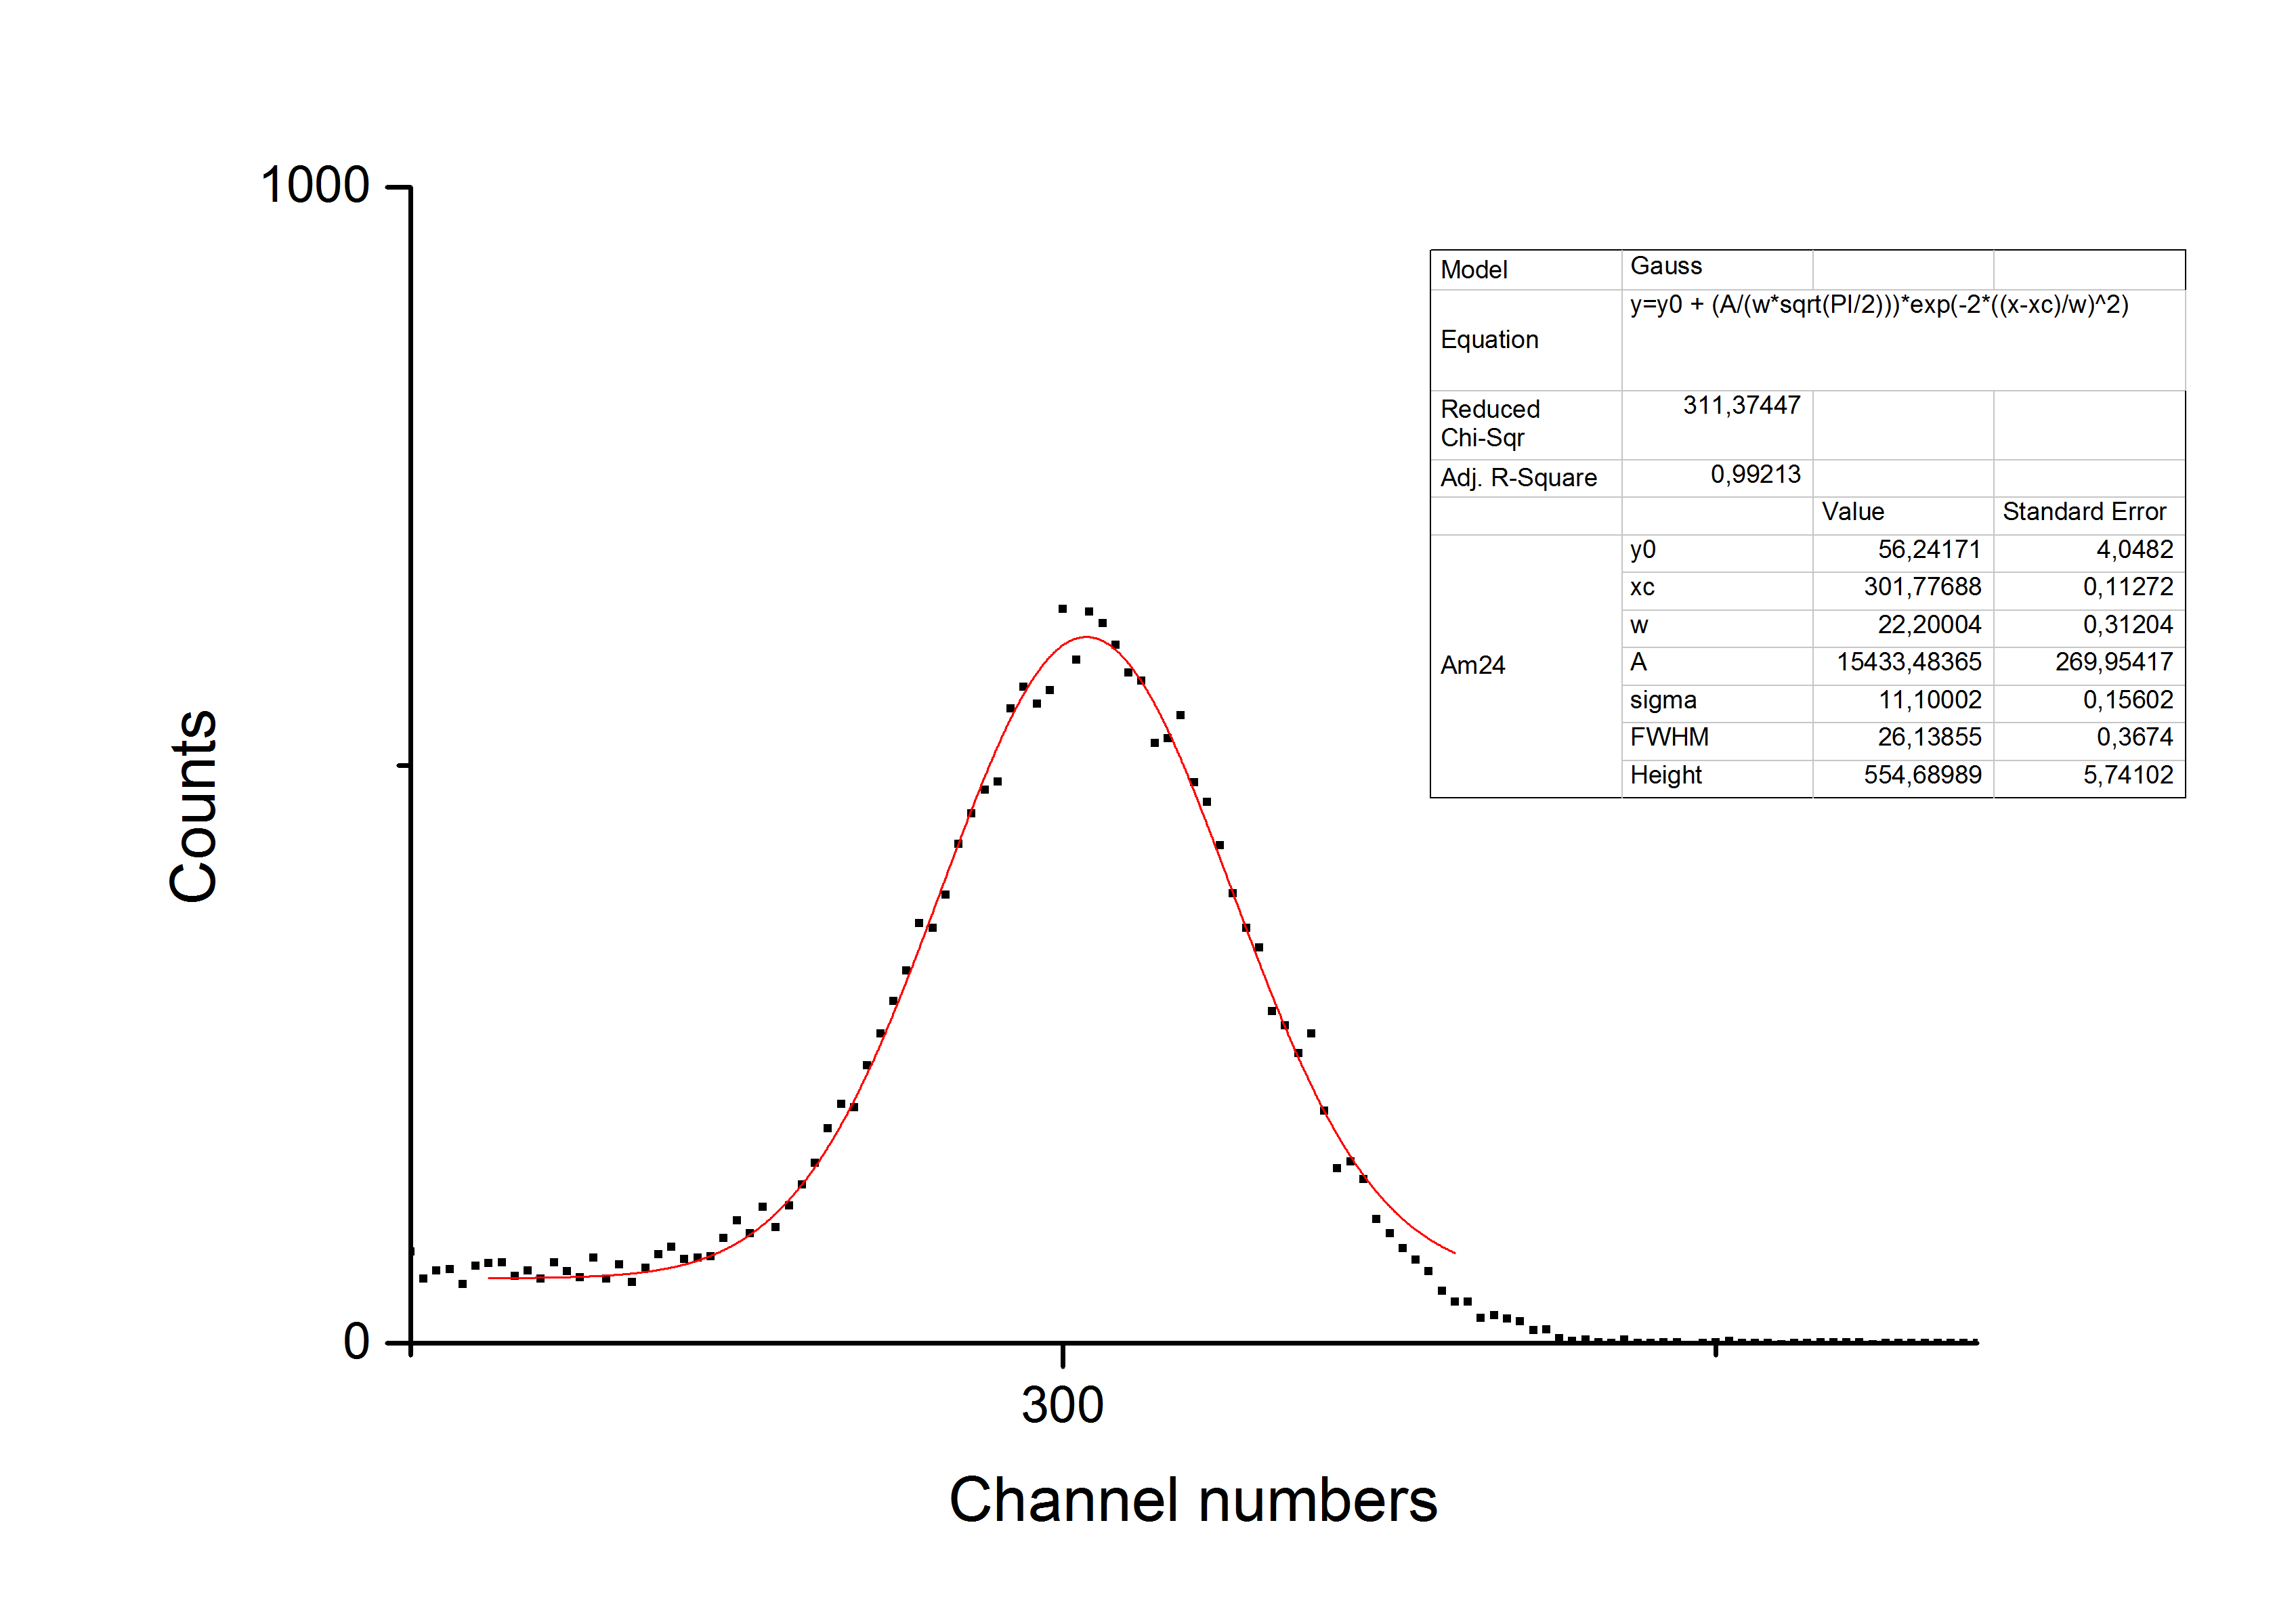
\includegraphics[scale=0.15]{Bilder/Teil3/Am_Si}
\caption{Am with Si-detector}
\label{fig:AmSi}
\end{center}
\end{figure}
%Inhaltsverzeichnis
\end{document}
